\documentclass[openany]{book}


% ==================================================================================================================================
% HEADER
% Documents packages, environements, page configuration

\usepackage[french]{babel}
\usepackage[T1]{fontenc}
\usepackage{ragged2e}
\usepackage{amsfonts}
\usepackage{systeme}
\usepackage{amsmath}
% \usepackage{amsthm}
\usepackage{amssymb}
\usepackage{bbm}
\usepackage{comment}
\usepackage{multicol}
\usepackage{lipsum} 
\usepackage{graphicx}
\usepackage{stmaryrd}
\usepackage{wrapfig}
\usepackage{colortbl}
\usepackage{cellspace}
\usepackage{ntheorem}
\usepackage{lmodern}
\usepackage{dsfont}
\usepackage{mathtools}
\usepackage{ragged2e}
\usepackage{tabularx}
\usepackage{titlepic}
\usepackage{fancyhdr}
\usepackage{caption}
\usepackage{xcolor}
\usepackage[T1]{fontenc}
\usepackage{lmodern}
\usepackage{listings}
\usepackage{tikz}
\usepackage{tkz-graph}
\usepackage{pgfplots}
\usepackage{mdframed}
\usepackage{xparse}
\usepackage{enumitem}
\usepackage{titlesec}
\usepackage{minitoc}  % Permet d'afficher une table des matières locale
\usepackage[top=3cm, bottom=3cm, left=3.5cm, right=3.5cm]{geometry}
\usepackage{etoolbox} % pour tester la présence d'un argument optionnel
\usepackage{nicematrix}
\usepackage{float}
\usepackage{optidef}
\usepackage{booktabs}
\usepackage{algorithm}
\usepackage{algpseudocode}
\usepackage{tcolorbox}
\usepackage[linkbordercolor=white]{hyperref}
\usepackage{caption}

% \pagestyle{empty}
\usetikzlibrary{cd}
\usetikzlibrary{patterns, arrows.meta}
\usetikzlibrary{angles,quotes}
\usetikzlibrary{intersections, 3d, calc}
\usetikzlibrary{automata, positioning} % Pour utiliser les motifs
\usepgfplotslibrary{fillbetween}


% - - - - - - - - - - - - - - - - - - - - - - - - - 
%                   PAGE SETTINGS
% - - - - - - - - - - - - - - - - - - - - - - - - - 

\setlength{\columnseprule}{1pt}               % ligne de séparation entre les colonnes
\def\columnseprulecolor{\color{black}}

\newcolumntype{C}{>{$\displaystyle}Sc<$}      % style d'affichage et taille 
\cellspacetoplimit=5pt                        % de la séparation entre colonnes
\cellspacebottomlimit=5pt

\renewcommand{\thechapter}{\arabic{chapter}}  % Set chapters numbers to 0

% Redéfinition de \part avec image optionnelle
\renewcommand{\part}[2][]{%
  \clearpage
  \refstepcounter{part} % incrémente le compteur de partie
  \addcontentsline{toc}{part}{\thepart\space #2} % ajoute au sommaire

  \begin{center}
    {\Huge\bfseries #2\par}
    \vspace{4em}  % Augmente l'écart à 2em
    \ifstrempty{#1}{}{%
      \includegraphics[]{#1}\par
    }
  \end{center}
  \vspace{2em}
}




% - - - - - - - - - - - - - - - - - - - - - - - - - 
%                 MATHS SHORTHANDS
% - - - - - - - - - - - - - - - - - - - - - - - - - 

\newcommand{\C}{\mathbb{C}}
\newcommand{\D}{\mathbb{D}}
\newcommand{\R}{\mathbb{R}}
\newcommand{\Q}{\mathbb{Q}}
\newcommand{\Z}{\mathbb{Z}}
\newcommand{\N}{\mathbb{N}}
\newcommand{\U}{\mathbb{U}}
\newcommand{\K}{\mathbb{K}}
\newcommand{\E}{\mathbb{E}}
\newcommand{\V}{\mathbb{V}}
\newcommand{\Lc}{\mathbb{L}}
\newcommand{\Fc}{\mathbb{F}}

\newcommand{\M}{\mathcal{M}}
\newcommand{\B}{\mathcal{B}}
\newcommand{\F}{\mathcal{F}}

%\renewcommand{\epsilon}{\varepsilon}
%\renewcommand{\phi}{\varphi}
%\renewcommand{\rho}{\varrho}

\renewcommand{\labelitemi}{\textbullet} % Utiliser des points noirs (•)

\newcommand{\myP}{\mathbb{P}}


% - - - - - - - - - - - - - - - - - - - - - - - - - 
%                 MODS NOTATION
% - - - - - - - - - - - - - - - - - - - - - - - - - 

\theorembodyfont{\upshape}

% Définir un environnement pour encadrer les définitions avec un titre
\NewDocumentEnvironment{definition}{O{}}
{
  \begin{mdframed}[linewidth=0pt,linecolor=gray,backgroundcolor=gray!10,roundcorner=5pt]
  \textbf{Définition}%
  \IfNoValueTF{#1}{}{~(\textbf{#1})} % Affiche le titre entre parenthèses et en gras s'il est fourni
  . % Point à la fin
}
{
  \end{mdframed}
}

% Définir un environnement pour encadrer les théorèmes avec un titre
\NewDocumentEnvironment{theorem}{O{}}
{
  \samepage
  \begin{mdframed}[linewidth=1pt,linecolor=darkgray,backgroundcolor=darkgray!10,roundcorner=5pt]
  \textbf{Théorème}%
  \IfNoValueTF{#1}{}{~(\textbf{#1})} % Affiche le titre entre parenthèses et en gras s'il est fourni
  . % Point à la fin
}
{
  \end{mdframed}
}

% Commande pour le carré en fin de preuve
\newcommand{\qed}{\hfill\ensuremath{\square}}

% Définir un environnement pour encadrer les corollaires
\NewDocumentEnvironment{corollary}{O{}}
{
  \begin{mdframed}[linewidth=1pt,linecolor=gray,backgroundcolor=gray!10,roundcorner=5pt]
  \textbf{Corollaire}%
  \IfNoValueTF{#1}{}{~(\textbf{#1})} % Affiche le titre entre parenthèses et en gras s'il est fourni
  . % Point à la fin
}
{
  \end{mdframed}
}


% Définir un environnement pour encadrer les critères
\NewDocumentEnvironment{criteria}{O{}}
  {
    \begin{mdframed}[linewidth=1pt,
                      linecolor=gray,
                      backgroundcolor=gray!10,
                      roundcorner=5pt
                      ]
    \textbf{Critère}%
    \IfNoValueTF{#1}{}{~(\textbf{#1})} % Affiche le titre entre parenthèses et en gras s'il est fourni
    . % Point à la fin
  }
  {
    \end{mdframed}
  }

% Définir un environnement pour encadrer les prorpiétés avec un titre
\NewDocumentEnvironment{prop}{O{}}
{
  \begin{mdframed}[linewidth=0pt,linecolor=gray,backgroundcolor=gray!10,roundcorner=5pt]
  \textbf{Propriété}%
  \IfNoValueTF{#1}{}{~(\textbf{#1})} % Affiche le titre entre parenthèses et en gras s'il est fourni
  . % Point à la fin
}
{
  \end{mdframed}
}
				

\theoremstyle{plain}
\newtheorem*{remark}{Remarque}
\newtheorem*{rappel}{Rappel}
\newtheorem*{notation}{Notation}
\newtheorem*{proposition}{Proposition}
\newtheorem*{lemma}{Lemme}
%\newtheorem*{prop}{Propriété}
\newtheorem*{proof}{Démonstration}
\newtheorem*{example}{Exemple}

% - - - - - - - - - - - - - - - - - - - - - - - - - 
%             Itemize env settings
% - - - - - - - - - - - - - - - - - - - - - - - - - 

\setlist[itemize,1]{label=\textbullet}
\setlist[itemize,2]{label=\textbullet}
\setlist[itemize,3]{label=\textbullet}
\setlist[itemize,4]{label=\textbullet}

% - - - - - - - - - - - - - - - - - - - - - - - - - 
%             lstlisting env settings
% - - - - - - - - - - - - - - - - - - - - - - - - - 

\definecolor{codegreen}{rgb}{0,0.6,0}
\definecolor{codegray}{rgb}{0.5,0.5,0.5}
\definecolor{codepurple}{rgb}{0.58,0,0.82}
\definecolor{backcolour}{rgb}{0.95,0.95,0.92}

\lstdefinestyle{mystyle}{
    backgroundcolor=\color{backcolour},   
    commentstyle=\color{codegreen},
    keywordstyle=\color{magenta},
    numberstyle=\tiny\color{codegray},
    stringstyle=\color{codepurple},
    basicstyle=\ttfamily\footnotesize,
    breakatwhitespace=false,         
    breaklines=true,                 
    captionpos=b,                    
    keepspaces=true,                 
    numbers=left,                    
    numbersep=5pt,                  
    showspaces=false,                
    showstringspaces=false,
    showtabs=false,                  
    tabsize=2
}

\lstset{style=mystyle}

% - - - - - - - - - - - - - - - - - - - - - - - - - 
%             Tableofcontents settings
% - - - - - - - - - - - - - - - - - - - - - - - - - 


% Profondeur des mini-tables des matières
\setcounter{minitocdepth}{2}  % Jusqu’aux sous-sections
\setcounter{parttocdepth}{1}  % Jusqu’aux chapitres dans les parties

% Configurer l’apparence
\mtcsetrules{minitoc}{off}  % Désactiver les lignes pour les chapitres
\mtcsetrules{parttoc}{off}   % Désactiver les lignes pour les parties

% Si tu veux que la table principale n'affiche que les parties :
\setcounter{tocdepth}{1}  % N'afficher que les \part dans la table principale


% --- Numérotation logique unique sans l'afficher dans la TOC
\makeatletter
\renewcommand{\theHchapter}{\thepart.\arabic{chapter}}
\makeatother

% Numéros des équations par section
\numberwithin{equation}{section}

% - - - - - - - - - - - - - - - - - - - - - - - - - 
%                       TITLE
% - - - - - - - - - - - - - - - - - - - - - - - - - 

% Document Title
\title{Fiches de Cours Master IMA}
\author{Axel PIGEON}
\date{\today}


\begin{document}

% Activer les mini tables des matières
\dominitoc    % Active les tables des chapitres


% ==================================================================================================================================
% CONTENT


% Title Page
\begin{titlepage}
    \centering
    \vspace*{2cm}

    \Huge
    Fiches de Cours

    \huge 
    Master IMA

    \vspace{3.0cm}


    % \begin{center}
    %     \includegraphics[scale=0.7]{./images/titlepage.png}
    % \end{center}

    \vfill

    \LARGE
    Université de Toulouse III, Paul Sabatier

    \Large
    Années universitaires 2025-2027

    \vspace{0.8cm}

    \today
\end{titlepage}


\tableofcontents

\setlength{\parindent}{0pt}

% ==================================================================================================================================
% Introduction


% ==================================================================================================================================
% Inclusion Parts (Courses)

\part[images/part_probabilites.pdf]{Probabilités}
\setcounter{chapter}{0}
% ==================================================================================================================================
% Probabilités

% - - - - - - - - - - - - - - - - - - - - - - - - - 
%                       TITLE
% - - - - - - - - - - - - - - - - - - - - - - - - - 


% - - - - - - - - - - - - - - - - - - - - - - - - - 
%               Chapters Inclusion
% - - - - - - - - - - - - - - - - - - - - - - - - - 

\chapter{Chaînes de Markov}

\minitoc


% ========================================================================================================
% Introduction 

Jusqu'à maintenant, nous avons étudié des suites de variables aléatoires dites iid (indépendantes et 
identiquement distribuées). Ces propriétés nous ont permis de développer beaucoup d'outils pour les étudier 
tels que la loi forte des grands nombres ou le théorème central limite. 

Or nous n'utilisons pas beaucoup ce type de suite de variables aléatoires en simulation. En effet, ces propriétés 
plutôt fortes ne permettent pas de modéliser des phénomènes dont l'évolution est plus complexe. Nous allons donc 
continuer à étudier des suites de variables aléatoires mais en rajoutant des relations de dépendance entre celles-ci. 
Cela nous permettra de modéliser des systèmes dynnamiques au cours du temps plus complexes. 

% ========================================================================================================
% Définition et Généralités

\section{Définitions et Généralités}

On se place ici dans un espace probabilisé $(E, \mathcal(F), \myP)$  et $E$ un \emph{espace d'état}
fini ou dénombrable. On s'intéresse à une suite de variables aléatoires $(X_n)_{n \in \N}$ ou $X_k$ est 
l'état du système au temps $k$. 

\begin{definition}[Trajectoire]
    On appelle \emph{trajectoire du système} jusqu'au temps $n \in \N^*$ la donnée $(X_1, \dots, X_n)$. 
\end{definition}

\begin{definition}[Chaîne de Markov]
    On dit qu'une suite $(X_n)_{n \geqslant 0}$ est une \emph{chaîne de Markov} si elle 
    vérifie la \emph{propriété de Markov} : 
        \[ \forall n \in \N, \forall i_0, i_1, \dots, i_{n-1} \in E, \] 
        \[ \boxed{ \myP (X_{n+1} = j \; | \; X_n = i, X_{n-1} = i_{n-1}, \dots, X_0 = i_0) = \myP (X_{n+1} = j \; | \; X_n = i)} \]
\end{definition}

\begin{remark}
    Conditionnellement à l'état présent $\{X_n = i\}$, la probabilité d'arriver à l'état $\{X_{n+1} = j\}$ 
    à l'itération suivante ne dépend pas des évènnements du passé $\{X_0 = i_0, \dots, X_{n-1} = n-1\}$. 
    On parle \emph{d'abscence de mémoire}. 
\end{remark}

\begin{definition}[Chaîne de Markov Homogène]
    Soit $(X_n)_{n \geqslant 0}$ une chaîne de Markov. On dit qu'elle est \emph{homogène} si : 
        \[ \forall n \in \N, \forall i,j \in E, \quad \myP (X_{n+1} = j \; | \; X_n = i) = \myP(X_1 = j \; | \; X_0 = i) \]
    On se placera toujours dans ce cadre.
\end{definition}

\begin{remark}
    Une chaîne de Markov homogène est une chaîne de Markov où le temps ($n$) n'apparaît pas dans la probabilité de 
    passer d'un état à l'autre. 
\end{remark}

\begin{example}[Marche Aléatoire]
    On modélise le mouvement d'une particule sur une grille par une chaîne de Markov où $X_n$ représente 
    la position de la particule au temps $n \in  \N$. On considère que la particule se déplace sur une 
    seule dimension. Elle peut donc avancer d'une case ou reculer d'une case à chaque itération. On notera 
    $ p \in [0,1]$ la probabilité qu'elle avance et $1-p$ la probabilité qu'elle recule indépendament du passé. 
    
    Soit $ (\varepsilon_i)_{i \geqslant 0}$ à valeurs dans $\{-1, 1\}$ telle que : 
        \[ \myP( \varepsilon_i = 1) 1 - \myP( \varepsilon_i = -1) = p \in [0,1] \]
    la variable aléatoire qui représente le mouvement de la particule.  
    Déterminons la loi de $X_n$ :
        \[ 
            X_{n+1} = X_n + \varepsilon_{n+1} 
            = X_{n-1} + \varepsilon_n + + \varepsilon_{n+1} 
            = \dots 
            = \sum_{i=1}^{n} \varepsilon_i 
        \] 
    Montrons que c'est bien une chaîne de Markov : 
        \begin{align*}
            X_{n+1} &= X_n + \varepsilon_{n+1} \\ 
            &= \left( \sum_{i=1}^{n} \varepsilon_i \right) + \varepsilon_{n+1} \\ 
            &= \sum_{i=1}^{n+1} \varepsilon_i 
        \end{align*}
    où tous les $ \varepsilon_i, i \in \llbracket 1, n+1 \rrbracket $ sont indépendants. 
    On a donc : 
        \begin{align*}
            \myP(X_{n+1} = j \; | \; X_n = i, \dots, X_0 = i_0) &= \myP(X_n + \varepsilon_{n+1} = j \; | \; X_n = i, \dots, X_0 = i_0) \\ 
            &= \myP(i + \varepsilon_{n+1} = j \; | \; X_n = i, \dots, X_0 = i_0) \\ 
            &= \myP( \varepsilon_{n+1} = j - i) 
        \end{align*}

    On pourra alors s'intéresser au nombre de fois où une trajectoire passe par un point $n \in \N$. 
    La théorie des chaînes de Markov permet de répondre à ce genre de questions. 
\end{example}

Plus généralement, on peut construire récursivement des chaînes de Markov en déinissant un $X_0$ fixé ou tiré par une 
loi $ \pi_0$ puis en posant : 
    \[ X_{n+1} = f(X_n, \varepsilon_{n+1}) \]
où $( \varepsilon_i)$ est une suite de variables aléatoires iid et $f$ une fonction mesurable. 

\begin{definition}[Matrice de Transition]
    Soit $(X_n)_{n \geqslant 0}$ une chaîne de Markov. On définit la \emph{matrice de transition} $P$ 
    de la chaîne comme la matrice, potentiellement infinie, telle que : 
        \[ P(i,j) = \myP(X_1 = j | X_0 = i) \] 
    Ainsi le coefficient de la i-ème ligne et de la j-ème colonne correspond à la probabilité de passer 
    de l'état $i$ à l'état $j$ en une étape.   
\end{definition}

\begin{example}
    Soit $P \in \mathcal{M}_3(\R)$ la matrice de transition suivante : 
        \[ P = 
            \begin{pmatrix}
                1/4 & 3/4 & 0 \\ 
                0 & 1/2 & 1/2 \\ 
                1/2 & 0 & 1/2 
            \end{pmatrix}  \]
    On peut alors la représenter par un graphe pondéré orienté dont les noeuds représentent les 
    états au temps $i$ de la chaîne de Markov et les poids les probabilités de passer d'un état à l'autre en une étape. 
    
    \begin{figure}[h!]
        \centering
        \begin{tikzpicture}[->,>=stealth',auto,node distance=4cm, thick,
                            every loop/.style={min distance=10mm,in=45,out=135,looseness=10}]
            
            % Nodes placés avec des positions relatives
            \node[draw, circle] (1) {1};
            \node[draw, circle, right of=1] (2) {2};
            \node[draw, circle, below of=2] (3) {3};
            
            % Boucles avec labels
            \path (1) edge[loop above] node {$1/4$} (1);
            \path (2) edge[loop right] node {$1/2$} (2);
            \path (3) edge[loop below] node {$1/2$} (3);
            
            % Arêtes avec labels automatiques
            \path (1) edge node {$3/4$} (2);
            \path (2) edge node {$1/2$} (3);
            \path (3) edge node {$1/2$} (1);

        \end{tikzpicture}
        \caption{Graphe Orienté Pondéré de la matrice de transition $P$}
    \end{figure}
\end{example}

\begin{definition}[Matrice Stochastique]
    La matrice de transition $P$ est dite \emph{stochastique} si 
        \[ \forall i \in  E, \quad \sum_{j \in E} P(i,j) = 1 \] 
    (i.e si la somme des poids des arrêtes de tout noeud du graphe associé est égale à 1)
\end{definition}















\chapter{Espérances Conditionnelles}

\minitoc

% ========================================================================================================
% Introduction 

Dans ce court chapitre nous allons nous attarder sur la notion d'espérance. 
Jusqu'ici, ce n'était qu'un outil pour décrire la tendance d'une série 
de réalisations d'une variable aléatoire. Nous allons ici nous permettre de la conditionner 
pour en déduire des informations sur notre variable de départ. 

% ========================================================================================================
% Espérances conditionnelles de variables aléatoires discrètes  

\section{Espérances conditionnelles sur un espace d'états discret}

\subsection{Exemple Introductif}

Une entreprise souhaite effectuer un questionnaire de satisfaction en vue d'améliorer ses services. 
Pour chaque client, le résultat du sondage peut être représenté par une variable aléaoite $X$ 
à valeurs dans $E = \{1, \dots, 100\}$. le résultat du sondage sera la moyenne empirique des 
réponses et il donnera une bonne estimation de $ \mathbb{E}(X)$. 

Or, pour permettre de personnaliser un peu plus ses services, l'entreprise souhaite connaître 
les caractéristiques des clients ayant donné le même score au sondage. Par exemple, elle souhaite 
étudier les réponses moyennes des clients en fonction de leur âge, de leur sexe, etc... Par exemple 
si $Y$ est la variable aléatoire qui représente l'âge d'un client, on souhaite obtenir la probabilité 
qu'un client d'âge $y$ attribue la note de $x$. Ce sera donc la quantité suivante : 
    $$ \myP(X = x \mid Y = y) = \frac{ \myP(X = x, Y = y) }{ \myP(Y = y) } $$
que l'on appelle \emph{probabilité conditionnelle} de $x$ sachant $y$. On peut ainsi définir 
une nouvelle mesure de probabilités appelée \emph{probabilité conditionnelle} telle que, pour $y$ 
fixé, on ait : 
    $$ \myP(X = \bullet \mid Y) = \frac{ \myP(X = \bullet, Y = y) }{ \myP(Y = y) } $$ 
    $$ \sum_{x \in E} \myP(X = x \mid Y = y) = 1 $$  
Ainsi, dans notre exemple, la note moyenne des clients d'âge $y$ sera \emph{l'espérance conditionnelle} de 
$X$ sachant $Y = y$ définie par : 
    $$ \mathbb{E}(X \mid Y = y) = \sum_{x \in E} x \myP(X = x \mid Y = y) $$
On peut donc définir une fonction $h : E \longmapsto \overline{\R}$ telle que : 
    $$ h = \mathbb{E}(X \mid Y) \quad \text{i.e} \quad \forall y \in E, h(y) = \mathbb{E}(X \mid Y = y) $$   
À noter que $X$ et $Y$ ne sont pas nécessairement à valeurs dans le même ensemble. 

\begin{example}
    Considérons l'expérience aléatoire suivante. On lance un dé équilibré à 6 faces. Soit $y$ son résultat. 
    On lance ensuite $y$ fois une pièce de monnaie équilibrée. On cherche à déterminer le nombre moyen de 
    fois où on tombe sur Pile. 

    Pour cela, on pose $Y$ une variable aléatoire à valeurs dans $ \llbracket 1, 6 \rrbracket $ et, conditionnellement 
    à $\{Y = y\}$ on définit $X$ la variable aléatoire de loi $ \mathcal{B}(y,p)$ où $p$ est la probabilité de 
    faire Pile. On a alors : 
        $$ \forall k \in \llbracket 0, y \rrbracket , \quad \myP(X = k \mid Y = y) = \binom{k}{y} p^k (1-p)^{y-k} $$ 
    d'où $ \mathbb{E}(X \mid Y = y) = yp$ donc $ \mathbb{E}(X \mid Y) = pY$.    
\end{example}

\begin{prop}[Composition]
    Soient deux variables aléatoires discrètes $X$ et $Y$ on a l'égalité suivante : 
        $$ \mathbb{E}( \mathbb{E}(X \mid Y) ) = \mathbb{E}(X) $$  
\end{prop}

\begin{proof}
    Soient $X$ et $Y$ deux variables aléatoires respectivement à valeurs dans $E$ et $E'$. On a : 
        \begin{align*}
            \mathbb{E}( \mathbb{E}(X \mid Y) ) &= \sum_{y \in E'} \mathbb{E}(X \mid Y = y) \myP(Y = y) \quad \quad \text{(Théorème de transfert)} \\ 
            &= \sum_{y \in E'} \myP(Y = y) \left( \sum_{x \in E} x \myP(X = x \mid Y = y) \right) \\ 
            &= \sum_{y \in E} \sum_{x \in E} x \myP(X = x, Y = y) \\ 
            &= \sum_{x \in E} \sum_{y \in E} x \myP(X = x, Y = y) \\ 
            &= \sum_{x \in E} x \myP(X = x) \quad \quad \text{(Probabilités Totales)} \\
            &= \mathbb{E}(X) 
        \end{align*}
\end{proof}

\begin{proposition}
    Pour reprendre l'exemple précédent, on se donne maintenant $y \in E'$ l'âge d'une personne et 
    on cherche à savoir quelle réponse $x \in E$ cette personne a donnée au sondage. 
    On souhaite donc déterminer $X$ à partir des informations fournies par $Y$. 
    On cherche donc $h(Y)$, une variable aléatoire fonction de $Y$, qui minimise l'erreur quadratique moyenne :
    \[
        \inf_h \mathbb{E}\big[(X - h(Y))^2\big] 
        = \inf_h \left\{ \mathbb{E}(X^2) - 2\,\mathbb{E}[h(Y)X] + \mathbb{E}[h(Y)^2] \right\}.
    \]

    On a, par le théorème de transfert :
    \begin{align*}
        \mathbb{E}\big[h(Y)\mathbb{E}(X|Y)\big] 
        &= \sum_{y \in E'} h(y) \mathbb{E}(X \mid Y = y)\, \mathbb{P}(Y = y) \\ 
        &= \sum_{x \in E}\sum_{y \in E'} x\,h(y)\,\mathbb{P}(X = x, Y = y) \\ 
        &= \mathbb{E}\big[h(Y)X\big].
    \end{align*}

    On en déduit que 
    \[
        \mathbb{E}\big[h(Y)(X - \mathbb{E}[X|Y])\big] = 0.
    \]
    Cette relation peut être interprétée comme une \emph{orthogonalité} : 
    si l’on considère le produit scalaire défini sur les variables aléatoires par 
    \[
        \langle U, V \rangle = \mathbb{E}[UV],
    \]
    alors $X - \mathbb{E}[X|Y]$ est orthogonal à toute variable aléatoire de la forme $h(Y)$. 
    Cette interprétation sera approfondie dans la partie suivante.

    Ainsi :
    \begin{align*}
        \inf_h \Big\{ \mathbb{E}(X^2) - 2\,\mathbb{E}[h(Y)X] + \mathbb{E}[h(Y)^2] \Big\}
        &= \inf_h \Big\{ \mathbb{E}(X^2) - 2\,\mathbb{E}\big[h(Y)\mathbb{E}(X|Y)\big] + \mathbb{E}[h(Y)^2] \Big\} \\
        &= \inf_h \Big\{ \mathbb{E}(X^2) - \mathbb{E}\big[\mathbb{E}(X|Y)^2\big] 
           + \mathbb{E}\big[(h(Y) - \mathbb{E}(X|Y))^2\big] \Big\} \\
        &= \mathbb{E}(X^2) - \mathbb{E}\big[\mathbb{E}(X|Y)^2\big]
           + \inf_h \mathbb{E}\big[(h(Y) - \mathbb{E}(X|Y))^2\big].
    \end{align*}

    Le terme d'espérance est minimal lorsque $h(Y) = \mathbb{E}(X|Y)$, 
    ce qui prouve que l'espérance conditionnelle est la meilleure approximation quadratique de $X$ sachant $Y$.
\end{proposition}


% ========================================================================================================
% Définition de l'espérance conditionnelle

\section{Définition de l'espérence conditionnelle}

Cette section fait appel à beaucoup de connaissances de théorie de la mesure. 
Des rappels peuvent s'imposer. On se place ici dans un espace de variables aléatoires 
de carré intégrable $L^2( \Omega, \mathcal{A}, \myP )$. C'est un espace de Hilbert 
doté d'un produit scalaire : 
    $$ 
        \langle ., \rangle : 
            \begin{cases}
                (L^2( \Omega, \mathcal{A}, \myP ))^2 \longrightarrow \R \\ 
                (X,Y) \longmapsto \mathbb{E}(XY) 
            \end{cases}
    $$ 
et muni d'une norme quadratique : 
    $$ 
        \| .\|_2 : 
            \begin{cases}
                L^2( \Omega, \mathcal{A}, \myP ) \longrightarrow \R \\ 
                X \longmapsto \sqrt{ \mathbb{E}(X^2)}
            \end{cases}
    $$

\subsection{Généralités}

\begin{definition}[Tribu engendrée]
    Soit $( \Omega, \mathcal{A}, \myP)$ un espace de probabilité et $X : \Omega \longrightarrow \R$ une variable 
    aléatoire. On définit la tribu engendrée par $X$, notée $ \sigma(X)$, est la tribu engendrée par les sous-ensembles 
    de $ \Omega$ de la forme $ \{X \leqslant a\}, \forall a \in \R$. 

    \medskip 

    De même, $ \sigma(X)$ contient tout les évènnement de la forme $\{X \in B\}$ avec $B \in \mathcal{B}_\R$. Plus généralement, 
    on peut définir $ \sigma(X_1, \dots, X_n)$ pour une collection de $n$ variables aléatoire $X_1, \dots, X_n$.  
    Intuitivement, $ \sigma(X)$ contient toute l'information associée à la variable $X$. 
\end{definition}

\begin{definition}[Variable aléatoire mesurable par rapport à $X$]
    Soit $(\Omega, \mathcal{A}, \mathbb{P})$ un espace de probabilité et $X : \Omega \to \mathbb{R}$ une variable aléatoire. 
    Une variable aléatoire $Z : \Omega \to \mathbb{R}$ est dite \emph{mesurable par rapport à $X$} si elle est mesurable 
    pour la tribu $\sigma(X)$, c’est-à-dire si :
    \[
        \forall B \in \mathcal{B}_{\mathbb{R}}, \quad Z^{-1}(B) \in \sigma(X).
    \]
\end{definition}

\begin{lemma}
    Soient $Y,W$ deux variables aléatoires sur $( \Omega, \mathcal{A}, \myP)$ telles que $Y$ est à valeurs 
    dans $ (E, \mathcal{E} )$ et $W$ dans $(R, \mathcal{B}_\R)$. $W$ est mesurable par rappport à $ \sigma(Y)$ 
    si et seulement si il existe $f \in \mathcal{M}(E,\R) $ telle que $W = f(Y)$. 
\end{lemma}


\subsection{Espérance conditionnelle}

Nous allons maintenant définir l'espérance conditionnelle comme une projection orthogonale.

\begin{proposition}
    Soient $X, Y \in L^2(\Omega, \mathcal{A}, \mathbb{P})$. 
    On souhaite approcher $X$ par une variable aléatoire mesurable par rapport à $Y$. 
    D'après le lemme précédent, toute variable aléatoire mesurable par rapport à $Y$ 
    est de la forme $h(Y)$ avec une fonction borélienne $h : \mathbb{R} \to \mathbb{R}$.

    On cherche donc à approcher $X$ à partir des variables du sous-espace :
    \[
        \mathcal{H} = \{\, h(Y) \mid h \in L^2(\mathbb{R}, \mathcal{B}_{\mathbb{R}}, \mathbb{P}_Y) \,\}
        \subset L^2(\Omega, \mathcal{A}, \mathbb{P}).
    \]
    La variable aléatoire de $\mathcal{H}$ la plus proche de $X$ 
    est, par définition, le \emph{projeté orthogonal} de $X$ sur $\mathcal{H}$.
\end{proposition}

\begin{definition}[Espérance conditionnelle comme projection]
    Dans le même contexte que précédemment, 
    l'espérance conditionnelle $\mathbb{E}(X \mid Y)$ est le \emph{projeté orthogonal} 
    de $X$ sur le sous-espace $\mathcal{H}$ défini ci-dessus. 
    Elle est caractérisée par la relation d’orthogonalité :
    \[
        \forall h(Y) \in \mathcal{H}, 
        \quad \mathbb{E}\big[(X - \mathbb{E}(X \mid Y))\,h(Y)\big] = 0.
    \]
\end{definition}

On peut étendre cette définition au cas $L^1$ grâce au théorème suivant.

\begin{theorem}[Existence]
    Soit $X \in L^1(\Omega, \mathcal{A}, \mathbb{P})$ et 
    $\mathcal{F}$ une sous-tribu de $\mathcal{A}$. 
    Alors il existe une unique variable aléatoire $Z$, 
    mesurable par rapport à $\mathcal{F}$, telle que :
    \begin{enumerate}[label=\roman*)]
        \item $\mathbb{E}(|Z|) < \infty$, 
        \item pour tout $W \in L^\infty(\Omega, \mathcal{F}, \mathbb{P})$, on a
        \[
            \mathbb{E}(XW) = \mathbb{E}(ZW).
        \]
    \end{enumerate}
    On appelle $Z$ \emph{l'espérance conditionnelle} de $X$ sachant $\mathcal{F}$ 
    et on la note $\mathbb{E}(X \mid \mathcal{F})$.
\end{theorem}

\subsection{Pour les variables à densité}

\begin{rappel}[Loi jointe et lois marginales]
    Soit $(X,Y)$ un couple de variables aléatoires à densité de loi jointe $f_{X,Y}$. 
    La \emph{loi marginale} de $y$ par rapport à $x$ est obtenue par : 
        $$ f_Y(y) = \int_\R f_{X,Y}(x,y) \; dx $$ 
    de même pour la \emph{loi marginale} de $x$ : 
        $$ f_X(x) = \int_\R f_{X,Y}(x,y) \; dy $$
\end{rappel}

\begin{definition}[Probabilité Conditionnelle]
    De même que pour les variables discrètes, on définit la probabilité conditionnelle de $X$ par sa densité : 
        $$ f_{X \mid Y = y} = \frac{f_{X,Y}(x,y)}{f_Y(y)} $$
    Ainsi pour $y \in \R$ fixé tel que  $f_Y(y) > 0$, $f_{X \mid Y = y}$ définit une densité sur $\R$ 
    et on peut lui associer : 
        $$ \mathbb{E}(X \mid Y = y) = \int_\R x f_{X \mid Y = y} (x) \; dx $$ 
\end{definition}

\begin{definition}[Espérance Conditionnelle (Cas continu)]
    Soient deux variables aléatoires $X$ et $Y$ à densité de loi jointe $f_{X,Y}$. 
    On définit l'espérance conditionnelle de $X$ par rapport à $Y$ comme la fonction : 
        $$ h : y \longmapsto \mathbb{E}(X \mid Y = y) = \int_\R x f_{X \mid Y = y} (x) \; dx $$
\end{definition}

\begin{remark}
    La condition d'orthogonalité du théorème précédent se vérifie de la même façon. Pour $ h : \R \longrightarrow \R$ 
    bornée, on a : 
        \begin{align*}
            \mathbb{E}( \mathbb{E}( X \mid Y) h(Y)) &= \int_\R  f_Y(y) h(y) \mathbb{E}(X \mid Y = y) \; dy \\ 
            &= \int_\R f_Y(y) h(y) \left( \int_\R x f_{X \mid Y = y}(x) \; dx \right) \; dy \\ 
            &= \int_{\R^2} x h(y) f_{X \mid Y = y}(x) f_Y(y) \; dx dy \\ 
            &= \int_{\R^2} x h(y) f_{X, Y}(x, y) \; dx dy \\ 
            &= \mathbb{E}(Xh(Y)) 
        \end{align*}
\end{remark}

% ========================================================================================================
% Propriétés de l'espérance conditionnelle

\section{Propriétés de l'espérance conditionnelle}

Voyons à présent quelques propriétés de l'espérance conditionnelle. 
Soit $( \Omega, \mathcal{A}, \myP)$ un espace de probabilités. 

\begin{prop}[Calcul]
    Soit $ \mathcal{F}$ une sous-tribu de $ \mathcal{A}$ et $X \in L^1( \mathcal{A}, \myP)$ une variable aléatoire. 
    On a : 
    \begin{enumerate}[label=\roman*)]
        \item $\mathbb{E}( \bullet \mid \mathcal{F} ) $ est \emph{linéaire}. 
        \item si $X \geqslant 0$ alors $ \mathbb{E}(X \mid \mathcal{F} ) \geqslant 0$ {presque sûrement}. 
        \item si $X$ est $ \mathcal{F}$-mesurable alors $ \mathbb{E}(X \mid \mathcal{F} ) = X $ {presque sûrement}. 
    \end{enumerate}  
\end{prop}

\begin{prop}[Indépendance]
    Si $X$ est \emph{indépendante} de $ \mathcal{F}$ alors : 
        $$ \mathbb{E}(X \mid \mathcal{F} ) = \mathbb{E}(X) $$   
\end{prop}

\begin{remark}
    Soit $Y,X$ deux variables aléatoires sur $( \Omega, \mathcal{A}, \myP)$. 
    On pose $ \mathcal{F} = \sigma(Y)$. Dire que $X$ \emph{est indépendante de} $ \mathcal{F} $
    revient à dire que $X$ est indépendante de $Y$. On aura alors : 
        $$ \mathbb{E}(X h(Y)) \overset{\perp}{=} \mathbb{E}(X) \mathbb{E}(h(Y)) = \mathbb{E}( \mathbb{E}(X) h(Y) ) $$    
\end{remark}

Les théorèmes de convergence (monotone et dominée) de l'intégration sont toujours valables pour l'espérance 
conditionnelle. 

\begin{theorem}[Convergence Monotone]
    Soit $(X_n)_{n \in \N}$ une suite de variables aléatoires et $X$ dans $L^1( \mathcal{A}, \myP)$. 
    Si $X_n \underset{n \to \infty}{\longrightarrow} X$ p.s en croissant, alors : 
        $$ \boxed{\lim_{n \to \infty} \mathbb{E}(X_n \mid \mathcal{F}) = \mathbb{E}(X \mid \mathcal{F} )} \quad \text{p.s}  $$
\end{theorem}

\begin{theorem}[Convergence Dominée]
    Soit $(X_n)_{n \in \N}$ une suite de variables aléatoires et $X$ dans $L^1( \mathcal{A}, \myP)$. 
        $$ X_n \underset{n \to \infty}{\longrightarrow} X \; \text{p.s} \quad \text{{et}} \quad  \sup_n |X_n| \leqslant w \in L^1 $$ 
        $$ \Longrightarrow \mathbb{E}(X_n \mid \mathcal{F} ) \underset{n \to \infty}{\longrightarrow} \mathbb{E}(X \mid \mathcal{F} ) $$
\end{theorem}

\begin{theorem}[Inégalité de Jensen]
    Soit $g : \R \longrightarrow \R$ une fonction \emph{convexe} et $X \in L^1( \mathcal{A}, \myP)$. Alors : 
        $$ \mathbb{E}(g(X) \mid \mathcal{F} ) \geqslant g( \mathbb{E}(X \mid \mathcal{F} ) ) $$ 
\end{theorem}

\begin{proposition}
    Soient $X \in L^1( \mathcal{A}, \myP)$ et $ \mathcal{F}, \mathcal{G} $ deux sous-tribus de 
    $ \mathcal{A}$. Alors : 
    \begin{enumerate}[label={\roman*)}]
        \item Si $ \mathcal{F} \subset \mathcal{G}$ (i.e $ \mathcal{G}$ contient plus d'informations 
            que $ \mathcal{F}$) alors : 
                $$ \mathbb{E}( \mathbb{E}(X \mid \mathcal{G} ) \mid \mathcal{F} ) = \mathbb{E}(X \mid \mathcal{F} )  $$
            \emph{(Puisque $ \mathcal{F}$ contient moins d'information que $ \mathcal{G}$, projeter $X$ sur 
            $ \mathcal{G}$ puis sur $ \mathcal{F}$ revient directement à projeter $X$ sur $ \mathcal{F}$)}. 
        \item Si $ \mathcal{F}$ est indépendante de $ \mathcal{G}$ et $X \perp \mathcal{G}$, alors : 
            $$ \mathbb{E}(X \mid \sigma( \mathcal{F}, \mathcal{G})) = \mathbb{E}(X \mid \mathcal{F}) $$ 
        \emph{(Rajouter une information $ \mathcal{G}$ qui n'a rien à voir avec l'expérience ne permet pas 
        d'améliorer la prédiction $ \mathbb{E}(X \mid \mathcal{F}))$}. 
    \item Soit $Y$ une variable aléatoire mesurable par rapport à $ \mathcal{F}$ et que 
        $ XY \in L^1( \mathcal{A}, \myP)$, alors : 
            $$ \mathbb{E}(XY \mid \mathcal{F}) = Y \mathbb{E}(X \mid \mathcal{F}) $$
        \emph{(Si $Y$ ne dépend que de l'information contenue dans $ \mathcal{F}$, alors 
        sa meilleure estimation $ \mathbb{E}(Y \mid \mathcal{F})$ est elle-même.)}
    \end{enumerate} 
\end{proposition}

% \subsection{Linéarité}

% Pour toutes variables aléatoires $X, Y \in L^1$ et pour tous réels $a, b \in \mathbb{R}$, on a :
% \[
%     \mathbb{E}(aX + bY \mid \mathcal{F}) 
%     = a\,\mathbb{E}(X \mid \mathcal{F}) + b\,\mathbb{E}(Y \mid \mathcal{F}).
% \]
% Cette propriété découle directement de la linéarité de l’espérance classique et du fait que la définition
% de $\mathbb{E}(X \mid \mathcal{F})$ repose sur des égalités d’espérance vis-à-vis de variables mesurables
% par rapport à $\mathcal{F}$.

% \subsection{Monotonicité}

% Si $X, Y \in L^1$ et $X \leq Y$ presque sûrement, alors :
% \[
%     \mathbb{E}(X \mid \mathcal{F}) \leq \mathbb{E}(Y \mid \mathcal{F}) \quad \text{p.s.}
% \]
% Cette propriété est une conséquence du théorème de la convergence monotone et de la positivité de l'espérance.

% \subsection{Caractère de projection}

% Si $X$ est $\mathcal{F}$-mesurable, alors :
% \[
%     \mathbb{E}(X \mid \mathcal{F}) = X.
% \]
% Autrement dit, conditionner une variable déjà déterminée par $\mathcal{F}$ ne modifie pas sa valeur.

% De plus, si $\mathcal{F}_1 \subset \mathcal{F}_2$, on a :
% \[
%     \mathbb{E}(\mathbb{E}(X \mid \mathcal{F}_2) \mid \mathcal{F}_1)
%     = \mathbb{E}(X \mid \mathcal{F}_1),
% \]
% ce qu’on appelle la \emph{propriété de la tour}.

% \subsection{Indépendance}

% Si $X$ est indépendante de $\mathcal{F}$, alors :
% \[
%     \mathbb{E}(X \mid \mathcal{F}) = \mathbb{E}(X).
% \]
% En effet, les informations contenues dans $\mathcal{F}$ n’apportent aucune connaissance supplémentaire sur $X$.

% \subsection{Inégalité de Jensen}

% Si $\varphi : \mathbb{R} \to \mathbb{R}$ est une fonction convexe et $X \in L^1$, alors :
% \[
%     \varphi\big(\mathbb{E}(X \mid \mathcal{F})\big)
%     \leq \mathbb{E}\big(\varphi(X) \mid \mathcal{F}\big)
%     \quad \text{p.s.}
% \]
% Cette propriété généralise l’inégalité de Jensen classique au cadre conditionnel.

% \subsection{Cas particulier : conditionnement par une variable aléatoire}

% Lorsque $\mathcal{F} = \sigma(Y)$, toutes les propriétés précédentes s’écrivent avec la notation abrégée
% $\mathbb{E}(X \mid Y)$, par exemple :
% \[
%     \mathbb{E}(\mathbb{E}(X \mid Y)) = \mathbb{E}(X),
%     \quad \text{et} \quad
%     \mathbb{E}(Xh(Y)) = \mathbb{E}(\mathbb{E}(X \mid Y)h(Y)).
% \]

% \begin{remark}
%     La dernière égalité correspond précisément à la relation d’orthogonalité démontrée plus haut :
%     \[
%         \mathbb{E}\big[(X - \mathbb{E}(X \mid Y))\,h(Y)\big] = 0,
%     \]
%     pour toute fonction bornée $h : \mathbb{R} \to \mathbb{R}$.
% \end{remark}


% ========================================================================================================
% Processus Aléatoires

\section{Processus aléatoires - Filtrations}

Les seuls processus que nous avons vu jusqu'à présent sont des suites de variables aléatoires 
indexées par le temps tels que les chaînes de Markov. 
Nous allons ici essayer de généraliser cette notion en introduisant la notion de \emph{filtration}. 

\begin{definition}[Filtration]\label{def:filtration}
    Soit $( \Omega, \mathcal{A}, \myP)$ un espace probabilisé. Une \emph{filtration} de cet espace 
    est une suite \emph{croissante} de tribus $ ( \mathcal{F}_n)_{n \in \N}$ telles que : 
        $$ \mathcal{F}_1 \subset \mathcal{F}_2 \subset \dots \subset \mathcal{A} $$ 
    Une filtration d'un processus sera donc l'information disponible jusqu'au temps $n$ 
    de ce processus. Sa croissance vient du fait que le processus accumule de l'information 
    au cours de son évolution. 

    \medskip

    On parlera ainsi d'espace de probabilité filtré, noté $ ( \Omega, \mathcal{A}, \mathcal{F}, \myP)$. 
\end{definition}

Dans le cadre précédent de l'études des chaînes de Markov, nous avons étudié des suites $(X_n)_{n \in \N}$ 
à valeurs dans $ (\R, \mathcal{B}_\R)$. On se concentrera donc sur l'étude des filtrations de cet espace mesurable. 

Nous pouvons bien sûr réexprimer les chaînes de Markov à l'aide des filtrations en définissant la notion de 
\emph{filtration naturelle} d'une chaîne de Markov. 

\begin{definition}[Filtration Naturelle]
    Soit $(X_n)_{n \in \N}$ une chaîne de Markov sur $( \Omega, \mathcal{A}, \myP)$ valeurs dans $(E, \mathcal{E})$. Sa filtration naturelle est 
    la suite croissante de sous-tribus $ \mathcal{F}_n$  de $ \mathcal{A}$ telles que : 
        \begin{equation}\label{def:filtration-naturelle}
            \forall n \in \N, \quad \mathcal{F}_n = \sigma(X_0, \dots, X_n)
        \end{equation} 
    dans le cas où $E$ est discret, on aura donc que : 
        $$ \forall n \in \N, \quad \mathcal{F}_n = \sigma(\{X_0 = x_0, \dots X_n = x_n \mid \forall x_0, \dots, x_n \in E\}) $$ 
\end{definition}

\begin{remark}
    Soit $(X_n)_{n \in \N}$ une chaîne de Markov sur un espace d'états discret. On a donc définit 
    sa filtration naturelle comme : 
        $$ \forall n \in \N, \quad \mathcal{F}_n = \sigma(\{X_0 = x_0, \dots X_n = x_n \mid \forall x_0, \dots, x_n \in E\}) $$ 
    D'où $ \forall B \in \mathcal{E}$, par propriété de Markov, on a : 
        $$ \myP(X_{n+1} \in B \mid \mathcal{F}_n) = \myP(X_{n+1} \in B \mid X_n) $$ 
    qui est une variable aléatoire à valeurs dans $ (\R, \mathcal{B}_\R)$ qui dépend des valeurs prises par $ X_n$ 
    et dont la valeur est $\myP(X_{n+1} \in B \mid X_n = x_n)$ si $X_n = x_n$. 

    De plus, pour toute fonction mesurable $h : (E, \mathcal{E}) \to (\mathbb{R}, \mathcal{B}_\mathbb{R})$, 
    l'espérance conditionnelle de $h(X_{n+1})$ sachant $X_n$ est une variable aléatoire $\sigma(X_n)$-mesurable définie 
    par :
        $$ \mathbb{E}[h(X_{n+1}) \mid X_n] = g(X_n) $$
    où la fonction $g : (E, \mathcal{E}) \to (\mathbb{R}, \mathcal{B}_\mathbb{R})$ est donnée, dans le cas discret, par :
        $$ g(x_n) = \sum_{y \in E} h(y)\, \mathbb{P}(X_{n+1} = y \mid X_n = x_n) $$
\end{remark}

De même que précédement, on pourra dire qu'un processus est \emph{adapté} à une filtration... 

\begin{definition}[Processus Adapté - Processus Prévisible]
    Soit $( \Omega, \mathcal{A}, \myP)$ un espace de probabilité et $( \mathcal{F}_n)_{n \in \N}$ une filtration de cet espace. 
    Soit $(Y_n)_{n \in \N}$ un processus à valeurs dans $(E, \mathcal{E})$. 
    \begin{enumerate}[label={\roman*)}]
        \item  On dira que le processus $(Y_n)_{n \in \N}$ est \emph{adapté} à la filtration 
        $( \mathcal{F}_n)_{n \in \N}$ si pour tout $n \in \N$, $Y_n$ est $ \mathcal{F}_n$ mesurable. 
                $$ \text{i.e} \quad \forall n \in \N, \quad \forall A \in \mathcal{E}, \quad Y_n^{-1}(A) \in \mathcal{F}_n $$
        \item On dira que le processus $(Y_n)_{n \in \N}$ est \emph{prévisible} par la filtration 
        $( \mathcal{F}_n)_{n \in \N}$ si pour tout $n \in \N$, $Y_n$ est $ \mathcal{F}_{n-1}$ mesurable. 
            $$ \text{i.e} \quad \forall n \in \N, \quad \forall A \in \mathcal{E}, \quad Y_n^{-1}(A) \in \mathcal{F}_{n-1} $$
        par convention, on dira que $ \mathcal{F}_{-1} = \{ \emptyset, \Omega\}$. 
    \end{enumerate}
    La notion de \emph{prévision} signifie que l'on peut connaître $Y_n$ avant le temps $n$ grâce 
    aux informations contenues dans $ \mathcal{F}_{n_1}$. 
\end{definition}

La notion de filtration permet aussi de généraliser les temps d'arrêts. 

\begin{definition}[Temps d'arrêt]
    Un temps d'arrêt $T$ pour une filtration $ \mathcal{F}_n$ sur $( \Omega, \mathcal{A}, \myP)$ est une 
    variable aléatoire à valeurs dans $( \overline{\N}, \mathcal{P}( \overline{\N}))$ telle que : 
        \begin{align*}
            \forall n \in \ N, \quad  & \{T \leqslant n\} \in \mathcal{F}_n \\  
        \end{align*} 
    Pour être plus précis, cela revient à $ T^{-1} \{0, 1, 2, \dots, n\} = \{ \omega \in \Omega \mid T( \omega) \leqslant n\} \in \mathcal{F}_n$. 
\end{definition}


\chapter{Martingales}

\minitoc

% ========================================================================================================
% Introduction 

Nous définissons dans ce chapitre un nouveau type de processus aléatoires plus théorique 
que les chaînes de Markov. Ce sera un outil mathématique du fait de ses bonnes 
propriétés de convergence. Nous appelerons ces processus des Martingales dont l'espérance 
conditionnelle par rapport au passé restera constante. 

\medskip 

Dans tout ce chapitre, nous considérerons des processus aléatoires à valeurs dans $\R$. 

% ========================================================================================================
% Généralités

\section{Généralités}

\subsection{Définition et exemples}

\begin{definition}[Martingale]
    Soit $( \Omega, \mathcal{A}, \mathcal{F}, \myP)$ un espace de probabilité filtré 
    et $(X_n)_{n \in \N}$ un processus aléatoire intégrable. On dira que $(X_n)_{n \in \N}$ est 
    \begin{enumerate}[label=\roman*)]
        \item une \emph{martingale} par rapport à $ (\mathcal{F}_n)_{n \in \N}$ si : 
            \begin{equation}\label{definition:martingale}
                \forall n \geqslant 1, \quad \mathbb{E}(X_n \mid \mathcal{F}_{n-1}) = X_{n-1}
            \end{equation}
        \item une \emph{sur-martingale} par rapport à $ (\mathcal{F}_n)_{n \in \N}$ si : 
            \begin{equation}
                \mathbb{E}(X_n \mid \mathcal{F}_{n-1}) \leqslant X_{n-1}
            \end{equation}
        \item une \emph{sous-martingale} par rapport à $ (\mathcal{F}_n)_{n \in \N}$ si : 
            \begin{equation}
                \mathbb{E}(X_n \mid \mathcal{F}_{n-1}) \geqslant X_{n-1}
            \end{equation}
    \end{enumerate}
\end{definition}

\begin{example}[Marche aléatoire simple]
    Soit $( \varepsilon_n)_{n \in \N}$ une suite indépendantes de variables aléatoires 
    à valeurs dans $(E, \mathcal{E})$ telles que $ \mathbb{E}( \varepsilon_n) = 0$ pour tout $n$. 
    On définit une marche aléatoire sur $E$ comme la suite $(S_n)_{n \in \N}$ telle que : 
        $$ S_0 = 0 \quad \forall n \geqslant 1, \; S_n = \sum_{k=1}^{n} \varepsilon_k $$ 
    $(S_n)_{n \in \N}$ est une martingale pour la filtration $ \mathcal{F}_n = \sigma( \varepsilon_1, \dots, \varepsilon_n)$. 
    En effet, on a : 
        \begin{align*}
            \mathbb{E}(S_{n+1} \mid \mathcal{F}_n) &= \mathbb{E}(S_n + \mathcal{E}_{n+1} \mid \mathcal{F}_n) \\ 
            &= \mathbb{E}(S_n \mid \mathcal{F}_n) + \mathbb{E}( \varepsilon_{n+1} \mid \mathcal{F}_n) 
        \end{align*}
    Or $ \varepsilon_{n+1} \perp \varepsilon_0, \dots, \varepsilon_n$ donc $ \mathbb{E}( \varepsilon_{n+1} \mid \mathcal{F}_n) = 0 $ d'où 
        $$ \mathbb{E}( S_{n+1} \mid \mathcal{F}_n) = \mathbb{E}(S_n) = S_n $$ 
    c'est donc bien une martingale par définition. On peut remarquer que si $ \mathbb{E}(S_n) \geqslant 0$, alors 
    $(S_n)_{n \in \N}$ est une sous-martingale. 
\end{example}


\begin{remark}
    Si $ \mathbb{E}( \varepsilon_n) \geqslant 0, \forall n \in \N$ alors : 
        $$ \mathbb{E}( S_{n+1} \mid \mathcal{F}_n) = S_n + \mathbb{E}( \varepsilon_{n+1}) \geqslant S_n $$ 
    donc $(S_n)_{n \in \N}$ serait une sous-martingale. 
\end{remark}

\begin{example}[Multiplicatif]
    Soit $( \varepsilon_i)_{i \in \N}$ une suite indépendante de variables aléatoires telles que $ \mathbb{E}( \varepsilon_i) = 1$ pour 
    tout $ i \in \N$. Posons : 
        $$ M_0 = 1 \quad \text{et} \quad \forall n \in \N, \; M_n = \prod_{i = 1}^{n} \varepsilon_i $$ 
    et $ \mathcal{F}_n = \sigma ( \varepsilon_1, \dots, \varepsilon_n)$. Montrons que $(M_n)_{n \in \N}$ est une 
    martingale. Pour tout $ n \in \N$, on a : 
        \begin{align*}
            \mathbb{E}(M_{n+1} \mid \mathcal{F}_n) &= \mathbb{E} \left( \varepsilon_{n+1} \times M_n \mid \mathcal{F}_n\right) \\ 
            &= M_n \times \mathbb{E}( \varepsilon_{n+1} \mid \mathcal{F}_n) \\
            &= M_n \times \mathbb{E}( \varepsilon_{n+1}) \\ 
            &= M_n 
        \end{align*}
    Par définition, $(M_n)_{n \in \N}$ est donc une martingale. 
\end{example}

\begin{example}[Lien avec les chaînes de Markov]
    On peut généraliser les chaînes de Markov en tant que Martingales grâce à l'utilisation de fonctions harmoniques. 
    Soit $(X_n)_{n \in \N}$ sur un espace d'états discret $E$ et de matrice de transition $P$. Une fonction 
    harmonique $h : E \longrightarrow \R$ vérifie : 
        $$ \forall x \in E, \quad h(x) = \sum_{y \in E} P(x,y)h(y) $$ 
    c'est donc un \emph{vecteur propre à droite} pour $P$. Supposons de plus que $ \forall n \in \N, h(X_n) \in L^1(\R)$. 
    Alors $(h(X_n))_{n \in \N}$ sera une martingale pour la filtration $( \mathcal{F}_n)_{n \in \N}$ associée à $(X_n)_{n \in \N}$. 
    En effet, pour tout $ n \in \N$, on a : 
        \begin{align*}
            \mathbb{E}(h(X_{n+1}) \mid \mathcal{F}_n) &= \mathbb{E}(h(X_{n+1}) \mid X_n) \\ 
            &= \sum_{y \in E} \mathbb{E}(h(X_{n+1}) \mathbbm{1}_{X_{n+1} = y} \mid X_n ) \\ 
            &= \sum_{y \in E} \myP(X_{n+1} = y \mid X_n) \\ 
            &= \sum_{y \in E} P(X_n,y) \\ 
            &= h(X_n)
        \end{align*}
\end{example}

\begin{proposition}[Généralisation de la définition]
    Soit $(M_n)_{n \geqslant 0}$ une martingale pour une filtration $ \mathcal{F}_n$ alors : 
        \begin{equation}\label{proposition:generalisation-definition}
            \forall n \in \N, \forall k \geqslant 1, \quad \boxed{ \mathbb{E}(M_{n +k} \mid \mathcal{F}_n) = M_n}
        \end{equation}
\end{proposition}

\begin{proof}
    Par récurrence sur $k$, on a :
    \begin{itemize}
        \item \textbf{Initialisation} : pour $k = 1$ c'est la définition. 
        \item \textbf{Hérédité} : soit $k \geqslant 1$ tel que : 
            $$ \mathbb{E}(M_{n+k} \mid \mathcal{F}_n) = M_n$$ 
        alors : 
            \begin{align*}
                \mathbb{E}(M_{n + k + 1} \mid \mathcal{F}_n) &= \mathbb{E}( \mathbb{E}(M_{n+k+1} \mid \mathcal{F}_n) \mid \mathcal{F}_n) \\ 
                &= \mathbb{E}(M_{n+1} \mid \mathcal{F}_n) = M_n 
            \end{align*}
    \end{itemize}
\end{proof}

\begin{remark}
    La proposition précédente nous donne une relation de récurrence pour les espérances : 
        $$ \forall n \in \N, \forall k \geqslant 1, \quad \mathbb{E}( \mathbb{E}(M_{n+k} \mid \mathcal{F}_n)) = \mathbb{E}(M_n) $$ 
    or $ \mathbb{E}( \mathbb{E}(M_{n+k} \mid \mathcal{F}_n)) = \mathbb{E}(M_{n+k})$ d'où : 
        $$ \mathbb{E}(M_{n+k}) = \mathbb{E}(M_n) $$ 
        $$ \iff \boxed{ \mathbb{E}(M_n) = \mathbb{E}(M_0)} $$ 
    Nous essaierons par la suite de généraliser cette proposition pour des temps aléatoires. 
\end{remark}

\subsection{Lien Martingale et sous-martingale}

Pour rappel, une sous-martingale est un processus $(Y_n)$ adapté à la filtration $ \mathcal{F}_n$ tel que : 
    $$ \mathbb{E}(Y_{n+1} \mid \mathcal{F}_n) \geqslant Y_n $$ 
De plus, pour une fonction convexe $g : \R \longrightarrow \R$, pour $X \in L^1( \mathcal{A}, \myP)$
et $ \mathcal{F}$ une sous-tribu de $ \mathcal{A}$, l'inégalité de Jensen nous donne 
    $$ \mathbb{E}(g(X) \mid \mathcal{F}) \geqslant g( \mathbb{E}(X \mid \mathcal{F})) $$ 
Nous pouvons donc faire le lien entre les martingales et les sous-martingales. 

\begin{corollary}[Inégalité de Jensen]\label{corollary:inegalite-jensen}
    Soit $(M_n)_{n \in \N}$ une martingale pour une filtration $ (\mathcal{F}_n)_{n \geqslant 0}$. 
    Soit $g : \R \longrightarrow \R$ \emph{convexe} telle que $g(M_n) \in L^1$ pour tout $n \in \N$.
    Alors $(g(M_n))_{n \in \N}$ est une sous-martingale. 
\end{corollary}

\begin{proof}
    On a facilement $ \mathbb{E}(g(M_{n+1}) \mid \mathcal{F}_n) \geqslant g( \mathbb{E}(M_{n+1} \mid \mathcal{F}_n)) = g(M_n)$. 
\end{proof}

\begin{example}[Marche aléatoire]
    Soit $( \varepsilon_i)_{i \geqslant 0}$ une suite idd de variables aléatoires telles que : 
        $$ \forall i \in \N, \quad \mathbb{E}( \varepsilon_i) = 0 \; \text{ et } \; \varepsilon_i^2 \in L^1 $$ 
    Posons $ S_n = \sum_{i=1}^{n} \varepsilon_i$ et $ \mathcal{F}_n = \sigma( \varepsilon_1, \dots \varepsilon_n)$. 
    $(S_n)_{n \geqslant 0}$ est donc une martingale pour $ \mathcal{F}_n$ (voir exemple précédent). D'après le 
    corollaire de l'inégalité de Jensen, $(S_n^2)_{n \geqslant 0}$ est une sous-martingale. On a donc : 
        $$ \mathbb{E}(S_{n+1}^2 \mid \mathcal{F}_n) \geqslant \mathbb{E}(S_n^2) $$ 
        $$ \iff \mathbb{E}(S_{n+1}^2) \geqslant \mathbb{E}(S_n^2) $$ 
    On a donc une suite croissante d'espérances et : 
        $$ \mathbb{E}(S_n^2) = \mathbb{E} \left( \left(\sum_{i=1}^{n} \varepsilon_i\right)^2 \right) = n \mathbb{E}( \varepsilon_1 ^2) $$ 
    Essayons donc de construire une martingale en posant : 
        $$ \forall n \in \N, \quad M_n = S_n^2 - \mathbb{E}(S_n^2) = S_n^2 - n \mathbb{E}( \varepsilon_1^2) $$ 
    On a donc, par définition : 
        $$ \mathbb{E}(M_{n+1} \mid \mathcal{F}_n) = \mathbb{E}(S_{n+1}^2 \mid \mathcal{F}_n) - (n+1)\mathbb{E}( \mathbb{E} (\varepsilon_1^2) \mid \mathcal{F}_n) $$ 
    or  
        \begin{align*}
            \mathbb{E}(S_{n+1}^2 \mid \mathcal{F}_n) &= \mathbb{E}\big[ ( S_n + \varepsilon_{n+1})^2 \mid \mathcal{F}_n \big] \\ 
            &= \mathbb{E}(S_n^2 \mid \mathcal{F}_n) + 2\mathbb{E}(S_n \varepsilon_{n+1} \mid \mathcal{F}_n) + \mathbb{E}( \varepsilon_{n+1}^2 \mid \mathcal{F}_n) \\ 
            &= S_n^2 + 2 S_n \mathbb{E}( \varepsilon_{n+1}) + \mathbb{E}( \varepsilon_{n+1}^2) \\ 
            &= S_n^2 + \mathbb{E}( \varepsilon_1^2) 
        \end{align*}
    d'où : 
        \begin{align*}
            \mathbb{E}(M_{n+1} \mid \mathcal{F}_n) = S_n^2 - n \mathbb{E}( \varepsilon_1^2) = M_n 
        \end{align*}
    On peut donc décomposer notre sous-martingale $S_n^2$ en une somme de martingale et ce que l'on appelera 
    un processus croissant en $n$ : 
        $$ S_n^2 = M_n + n \mathbb{E}( \varepsilon_1^2) $$ 
\end{example}

\begin{proposition}[Décomposition de Doob]
    Soit $(X_n)_{n \geqslant 0}$ une sous-martingale par rapport à une filtration $ \mathcal{F}_n$. 
    Alors il existe un unique couple de processus $(M_n)_{n \geqslant 0}$ et $(Z_n)_{n \geqslant 0}$ tels que: 
    \begin{enumerate}[label=\roman*)]
        \item $(M_n)_{n \geqslant 0}$ est une martingale pour $ \mathcal{F}_n$ 
        \item $Z_0 = 0$ et $Z_{n+1} \geqslant Z_n$ et $(Z_n)_{n \geqslant 0}$ est prévisible pour $ (\mathcal{F}_n)_{n \geqslant 0}$. 
    \end{enumerate}
    et : 
        \begin{equation}\label{eq:doob-inequality}
            \forall n \in \N, \quad \boxed{X_n = M_n + Z_n}
        \end{equation}
\end{proposition}

\begin{proof}
    Soit $(X_n)_{n \in \N}$ une sous-martingale. par rapport à $( \mathcal{F}_n)_{n \geqslant 0}$. On définit les 
    écarts : 
        $$ \forall n \in \N, \quad \Delta_n = X_{n+1} - X_n $$ 
    Posons $ M_0 = X_0$ et $Z_0 = 0$. On construit récursivement $(M_n)_{n \geqslant 0}$ et $(Z_n)_{n \geqslant 0}$ tels 
    que :
        $$ \forall n \in \N, \quad Z_n = \sum_{i=1}^{n} \mathbb{E}( \Delta_i \mid \mathcal{F}_{i-1}), \quad M_n = X_n - Z_n $$
    Montrons que des deux processus vérifient les hypothèses : 
    \begin{enumerate}[label=\roman*)]
        \item Par contruction, pour tout $ n \in \N$, on a $X_n = M_n + Z_n$. 
        \item Pour tout $i \in \llbracket 1, n \rrbracket$, $ \mathbb{E}( \Delta_i \mid \mathcal{F}_{i-1})$ est $ \mathcal{F}_{i-1}$ 
            mesurable et $Z_n$ est une somme de $i$ variables $ \mathcal{F}_{i-1}$ mesurables. Donc $(Z_n)_{n \geqslant 0}$ est 
            prévisible pour $( \mathcal{F}_n)_{n \geqslant 0}$. 
        \item Pour tout $n \in \N$, on a : 
            \begin{align*}
                Z_{n+1} - Z_n &= \mathbb{E}( \Delta_{n+1} \mid \mathcal{F}_n) \\ 
                &= \mathbb{E}(X_{n+1} \mid \mathcal{F}_n) - \mathbb{E}(X_n \mid \mathcal{F}_n) \\ 
                &= \mathbb{E}(X_{n+1} \mid \mathcal{F}_n) - X_n 
            \end{align*}
        or $X_n$ est une sous-martingale donc : 
            $$ \mathbb{E}(X{n+1} \mid \mathcal{F}_n) \Longrightarrow Z_{n+1} \geqslant Z_n $$ 
        Puisque $Z_0 = 0$, $(Z_n)_{n \in \N}$ est un processus croissant. 
    \end{enumerate}
    Montrons maintenant que $(M_n)_{n \in \N}$ est une martingale. 
    \begin{align*}
        \forall n \in \N, \mathbb{E}(M_{n+1} \mid \mathcal{F}_n) &= \mathbb{E}(X_{n+1} \mid \mathcal{F}_n) - \mathbb{E}(Z_{n+1} \mid \mathcal{F}_n) \\ 
        &= \mathbb{E}(X_{n+1} \mid \mathcal{F}_n) - Z_{n+1} \quad \\ 
        &= \mathbb{E}(X_{n+1} \mid \mathcal{F}_{n}) - Z_n - \mathbb{E}( \Delta_{n+1} \mid \mathcal{F}_n) \\ 
        &= \mathbb{E}(X_{n+1} \mid \mathcal{F}_{n}) - Z_n - (\mathbb{E}( \Delta_{n+1} \mid \mathcal{F}_n) - X_n) \\ 
        &= X_n - Z_n = M_n
    \end{align*}
    L'unicité se montre par récurrence sur $n$. Nous ne la ferons pas ici.
\end{proof}


% ========================================================================================================
% Stratégies et théorème d'arrêt

\section{Stratégies et théorème d'arrêt}

\begin{example}[Ruine du joueur]
    Considérons un joueur lors d'un jeu aléatoire constitué de $N$ parties. Lors de la partie 
    $n \leqslant N$, il mise une somme $ \Theta_n$ et il remporte la some $ \varepsilon_n \Theta_n$ où 
    $ \varepsilon_n = -1$ s'il perd et $ \varepsilon_n = 2$ s'il gagne. 

    \medskip

    Les variables $( \varepsilon_n)_{n \geqslant 0}$ dépendent du jeu, donc on peut construire une filtration 
    $ ( \mathcal{F}_n)_{n \geqslant 0}$ définie par $ \mathcal{F}_n = \sigma( \varepsilon_1, \dots \varepsilon_n)$. 
    On peut considérer que $( \varepsilon_n)_{n \in \N}$ sont iid. Par construction, $\Theta_n$ est $\mathcal{F}_{n-1}$-mesurable, donc prévisible.
    On définit alors le gain total du joueur après $n$ parties comme la variable : 
        $$ \forall n \leqslant N, \quad S_n = S_0 + \sum_{k=1}^{n} \Theta_k \varepsilon_k $$ 
\end{example}

Dans cette section, nous allons essayer de généraliser cette structure au travers des stratégies. 

\begin{proposition}
    Soit $(M_n)_{n \geqslant 0}$ une martingale pour la filtration $( \mathcal{F}_n)_{n \geqslant 0}$, 
    $ ( \Phi_n)_{n \geqslant 0}$ un processus prévisible et borné. le processus défini par :
        \begin{equation}\label{eq:not-optimal-strategy}
            X_0 = 0 \text{ et } \forall n \in \N, \quad X_n = \sum_{k=1}^{n} \Phi_k (M_k - M_{k-1})
        \end{equation}
    Alors $(X_n)_{n \in \N}$ est une martingale pour $( \mathcal{F}_n)_{n \geqslant 0}$. 
\end{proposition}

Cette proposition est fondamentale dans l'interprétation des martingales en tant que stratégies de jeu. 
En effet, elle nous montre que pour n'importe quel jeu initial d'espérance nulle $(M_n)_{n \in \N}$ (gain moyen), il n'existe 
aucune stratégie $( \Phi_n)_{n \in \N}$ permettant de modifier le gain moyen. 
Cette notion est traduite par le fait que $(X_n)_{n \in \N}$ reste une martingale. 

\begin{remark}
    Les martingales nous permettent de modéliser la plupart des stratégies. Par exemple, si l'on veut 
    modéliser une stratégie du type "le joueur mise jusqu'à avoir accumulé une certaine somme $ \lambda$", 
    alors on peut définir $T$ le temps d'arrêt tel que : 
        $$ T = \inf \{n \in \N \mid S_n \geqslant \lambda\} $$ 
    On posera donc : 
        $$ \forall n \in \N, \forall k \in \llbracket 1, n \rrbracket, \quad \Phi_k = \mathbbm{1}_{k \geqslant \lambda} \quad \text{et} 
        \quad X_n = \sum_{k=1}^{n} \Phi_k (M_k - M_{k-1}) $$  
\end{remark}

On souhaiterai aussi généraliser la notion de chaîne de Markov $(X_n)_{n \in \N}$ arrêtée par un temps d'arrêt $T$ 
définie par : 
    $$ 
        \forall n \in \N, \quad X_n = 
            \begin{cases}
                X_n \quad \text{si } n \leqslant T \\ 
                X_T \quad \text{sinon}  
            \end{cases}
    $$

\begin{proposition}[Martingale arrêtée]
    Ainsi, soit $(M_n)_{n \leqslant 0}$ une martingale pour la filtration $ \mathcal{F}_n$ $T$. 
    Soit $T$ un temps d'arrêt. On pose : 
        $$ \forall k \in \N, \quad \Phi_k = \mathbbm{1}_{\{T \geqslant n\}} $$ 
    L'évènnement $\{T \leqslant n\}$ est mesurable par rapport à $ \mathcal{F}_{n-1}$ car il se décompose 
    comme le complémentaire d'une intersection dénombrable d'évènnements $ \mathcal{F}_{n-1}$ mesurables : 
        $$ \{T \leqslant n\} = \overline{\{T \geqslant n\}} = \bigcap_{k = 1}^{n-1} \{T \not = k\} $$ 
    Le processus $ \Pi_k $ est donc prévisible pour la filtration $( \mathcal{F}_n)_{n \geqslant 0}$. 
    D'après la proposition \ref{eq:not-optimal-strategy}, le processus défini comme : 
        \begin{equation}\label{eq:martingale-arrete}
            \boxed{
                \forall n \in \N, \quad M_n = 
            \begin{cases}
                M_n \quad \text{si } n \leqslant T \\ 
                M_T \quad \text{ sinon }  
            \end{cases}
            }
        \end{equation}
\end{proposition}

\begin{theorem}[Arrêt (Doob)]\label{theorem:stop-doob-theorem}
    Soit $(M_n)_{n \geqslant 0}$ une martingale pour la filtration $( \mathcal{F}_n)_{n \in \N}$.
    Soit $T$ un temps d'arrêt pour $( \mathcal{F}_n)_{n \geqslant 0}$. 
    Si une des trois assertions suivante est vraie : 
    \begin{enumerate}[label=\roman*)]
        \item $T$ est borné p.s 
        \item $ T < \infty$ p.s et $(M_n)_{n \in \N}$ est borné. 
        \item Si $T \in L^1$ et : 
            \begin{equation}\label{eq:third-stop-condition}
                \sup_n \left| M_n - M_{n-1 }\right| = \sup_n \left| \Delta_{M_n}\right| \leqslant C \quad \text{p.s}  
            \end{equation}
    \end{enumerate}
    Alors $\boxed{ \mathbb{E}(M_T) = \mathbb{E}(M_0)}$.
\end{theorem}

Ce théorème nous permet donc de généraliser aux temps d'arrêt la proposition de généralisation de la 
définition des martingales \ref{proposition:generalisation-definition}.


\part[images/part_simulation.pdf]{Simulation Aléatoire}
\setcounter{chapter}{0}
% ==================================================================================================================================
% Simulation

% - - - - - - - - - - - - - - - - - - - - - - - - - 
%                       TITLE
% - - - - - - - - - - - - - - - - - - - - - - - - - 


% - - - - - - - - - - - - - - - - - - - - - - - - - 
%               Chapters Inclusion
% - - - - - - - - - - - - - - - - - - - - - - - - - 

\chapter{Simulation de variables aléatoires}

\minitoc 

% ========================================================================================================
% Introduction 

La simulation peut se définir comme la prédiction de l'évolution d'un système en résolvant des équations 
venues de domaines appliqués. 
La notion d'aléatoire vient du fait que l'on simule des phénomènes dont nous n'aurons que des informations imparfaites 
tels que des phénomènes de désintégration nucléaire ou de prévention des risques. Les utilisations 
possibles de la simulation sont : 
\begin{itemize}
    \item Étude d'un phénomène (ex : la trajectoire d'un avion dans des turbulences)
    \item L'estimation de caractéristiques d'un système (ex : déterminer les caractéristiques d'une simulation météo)
    \item Tester des hypothèses (ex : en médecine, on peut utiliser la simulation aléatoire pour déterminer à l'avance 
    les effets d'un médicament sur un patient.)
    \item La prise de décision dans un environement incertain. 
    \item Réaliser des expériences coûteuses voire impossibles (ex : effectuer des essais nucléaires informatiquement 
    en fonction des essais passés ou simuler une propagation virale dans une population). 
\end{itemize}
La simulation aléatoire est donc un outil rapide économique et contrôlé. 

\begin{definition}[Simuler une variable aléatoire]
    Simuler une variable aléatoire de loi $\mu$ consiste à produire un algorithme dont les réalisations donnent 
    des copies indépendantes d'une variable de loi $ \mu$. 
\end{definition}

La simulation aléatoire est impossible sans l'accès à des \emph{données aléatoires}. En pratique, on se contentera 
de données \emph{pseudo-aléatoires} tel que le nombre de secondes écoulées depuis le 01/01/1070, la température 
d'un processeur ou les dernières touches entrées avant l'exécution du programme. 
Ceci est obtenu en \texttt{Python} avec la fonction \texttt{rand()}.  Dans ce cours, on considère que chaque appel 
à cette fonction nous renvoie une variable iid de loi Uniforme sur $[0,1]$. 

Simuler une variable aléatoire consiste donc à construire un algorithme qui transforme un nombre fini de variables 
aléatoires idd de loi $ \mathcal{U}([0,1])$ en une variable aléatoire de loi $ \mu$ : 
    \[ \mathcal{U}([0,1]) \overset{\text{simulation}}{\longrightarrow} \mu \] 

% ========================================================================================================
% Simulation de variables aléatoires discrètes

\section{Simulation de variables aléatoires discrètes}

\begin{example}[Simuler une variable aléatoire de loi $ \mathcal{B}(p)$]
    Soit $X \sim \mathcal{U}([0,1])$ avec $p \in [0,1]$. Alors la variable $Y = \mathds{1}_{X \leqslant p}$  
    suit un loi de Bernouilli de paramètre $p$. 
        \[ \myP(Y = 1) = \myP(\mathds{1}_{X \leqslant p} = 1) = \myP(X \leqslant p) = p \]  
        \[ \myP(Y = 0) = 1 - p \] 
    On peut donc développer l'algorithme suivant :
    \begin{lstlisting}[language=Python]
def bernouilli(p): 
    x = rand()
    if u <= p: 
        return 1 
    return 0
    \end{lstlisting}
\end{example}

\begin{example}[Simuler une loi binomiale $ \mathcal{B}(n,p)$]
    Soient $(X_1, \dots, X_n)$ une suite de variables aléatoires iid de loi $ \mathcal{B}(n,p)$. 
    La variable $ Y := \sum_{n=1}^{n} X_i \sim \mathcal{B}(n,p)$ telle que : 
        \[ \myP(Y = k) = \binom{n}{k} p^k (1-p)^{n-k} \] 
    Il nous faut donc seulement générer la somme de $n$ variables aléatoires suivant une loi de Bernouilli. On a donc : 
        \begin{lstlisting}[language=Python]
def binom(n,p):
    s = 0 
    for i in range(n):
        s += 1 * (rand() <= p) 
    return s
    \end{lstlisting} 
\end{example}

On cherchera à développer des programmes qui terminent en temps fini. On préferera deux qui terminent 
en temps borné (comme \texttt{binom(n,p)}). 

\begin{proposition}
    Soit $(p_n)_{n \geqslant 1}$ une suite réelle positive telle que : 
        \[ \sum_{k=1}^{\infty} p_k = 1 \] 
    et $(x_n)$ une suite d'éléments d'un ensemble $E$. On définit la loi $ \mu$ par : 
        \[ \mu = \sum_{k=1}^{\infty} p_k \delta_{x_k} \] 
    si une variable aléatoire $X$ est de loi $ \mu$ on aura alors $ \myP(X = x_k) = p_k$. 
    On pose $f_0 = 0$ et $s_k = p_1 + \dots + p_k$. Soit $U$ une variable aléatoire de loi $ \mathcal{U}([0,1])$. 
    Alors la variable : 
        \[ Y = \sum_{k=1}^{\infty} x_n \times \mathds{1}_{s_{n-1} \leqslant U \leqslant s_k} \] 
    suit la loi $ \mu$. L'algorithme suivant simule une variable aléatoire de loi $ \mu$. 
    \begin{lstlisting}[language=Python]
def simulation_mu([p1, ..., pk],[x1, .., xk]): 
    u = rand() 
    s = p1 
    while u > s :
        i++ 
        s += pi 
    return xi 
    \end{lstlisting}  
\end{proposition}

\begin{proof}
    Pour tout $n \in \N$, on a :
        \[ \myP(s_{n-1} \leqslant U \leqslant s_n) = s_n - s_{n-1} = p_n \] 
    donc $ \myP(Y = x_n) = \myP(s_{n-1} \leqslant U \leqslant s_n) = p_n $.   
\end{proof}

\begin{example}[Simuler une loi de Poisson $ \mathcal{P}(\lambda)$ ]
    Pour rappel, si $X \sim \mathcal{P}(\lambda)$ alors : 
        \[ \forall k \in \N, \quad \myP(X = k) = e^{-\lambda} \frac{\lambda^k}{k !} \]  
    Posons $ p_k := e^{- \lambda} \frac{ \lambda^k}{k!}$. On remarque que : 
        \[ p_{k+1} = e^{- \lambda} \frac{ \lambda^{k+1}}{(k+1)!} = p_k \frac{ \lambda}{k+1} \] 
    On en déduis donc l'algorithme suivant : 

    \begin{lstlisting}[language=Python]
def poisson(lambda): 
    x = 0 
    p = exp(-\lamdba) 
    s = p 
    u = rand() 
    while u > s : 
        x += 1
        p = p * lambda / x 
        s += p 
    return x  
    \end{lstlisting}
\end{example}

\begin{example}[Loi uniforme]
    Simulons une loi uniforme sur $\{1, \dots, n\}$. 
    On a donc l'algorithme suivant : 

    \begin{lstlisting}[language=Python]
def uniforme(n):
    x = 1 
    s = x/n 
    u = rand() 
    while u > s : 
        x += 1
        s += 1/n 
    return x 

def uniforme(n):
    return ceil(n * rand(u))
    \end{lstlisting}
\end{example}

\begin{proposition}[Algorithme du Rejet]
    Soit $(E, \mathcal{E}, \mu)$ un espace probabilisé et $A \subset E$ un évènement tel que $\mu(A) > 0$. 
    La loi $\mu$ conditionnellement à $A$, notée $\mu_A$, est définie par :
    \[
        \mu_A(B) = \frac{\mu(A \cap B)}{\mu(A)}, \qquad B \in \mathcal{E}.
    \]
    Soit $(X_n)_{n \geqslant 1}$ une suite de variables aléatoires i.i.d. de loi $\mu$. 
    On pose :
    \[
        T := \inf \{ n \geqslant 1 \mid X_n \in A \},
    \]
    c'est-à-dire le rang du premier tirage appartenant à $A$.
    Alors :
    \begin{enumerate}
        \item $T \sim \mathcal{G}(\mu(A))$, c'est-à-dire
        \[
            \mathbb{P}(T = k) = (1 - \mu(A))^{k-1} \mu(A), \qquad k = 1,2,\dots
        \]
        \item $X_T \sim \mu_A$ (loi conditionnelle sur $A$)
        \item $X_T$ et $T$ sont indépendantes.
    \end{enumerate}
\end{proposition}

\begin{proof}
    Soit $B \in \mathcal{E}$ et $k \geqslant 1$. On calcule :
    \begin{align*}
        \mathbb{P}(X_T \in B, T = k) 
        &= \mathbb{P}(X_k \in B, T = k) \\
        &= \mathbb{P}(X_1 \notin A, \dots, X_{k-1} \notin A, X_k \in A, X_k \in B) \\
        &= \mathbb{P}(X_1 \notin A)^{k-1} \times \mathbb{P}(X_1 \in A \cap B) \\
        &= (1 - \mu(A))^{k-1} \mu(A) \frac{\mu(A \cap B)}{\mu(A)} \\
        &= \underbrace{(1 - \mu(A))^{k-1} \mu(A)}_{\mathbb{P}(T = k)}
           \underbrace{\frac{\mu(A \cap B)}{\mu(A)}}_{\mu_A(B)}.
    \end{align*}
    On en déduit :
    \begin{itemize}
        \item $\mathbb{P}(T = k) = (1 - \mu(A))^{k-1} \mu(A)$ (loi géométrique)
        \item $\mathbb{P}(X_T \in B) = \mu_A(B)$
        \item $\mathbb{P}(X_T \in B, T = k) = \mathbb{P}(T = k) \mathbb{P}(X_T \in B)$, donc $T$ et $X_T$ sont indépendantes.
    \end{itemize}
\end{proof}


\paragraph{Interprétation.}
L'algorithme du rejet décrit la procédure suivante :
\begin{enumerate}
    \item Tirer $X_1, X_2, \dots$ de manière indépendante selon la loi $\mu$.
    \item Rejeter tout tirage $X_n \notin A$ et recommencer.
    \item Accepter le premier $X_T \in A$ : sa loi est exactement $\mu_A$.
\end{enumerate}

Ainsi :
\begin{itemize}
    \item $T$ représente le nombre de tirages nécessaires avant d'obtenir un succès.
    \item $X_T$ est la valeur de ce premier succès, distribuée comme $\mu$ conditionnellement à $A$.
    \item $T$ et $X_T$ sont indépendants : le temps d'attente n'influence pas la valeur obtenue.
\end{itemize}

\begin{example}
    Si $E$ est l'ensemble des notes d'étudiants, $\mu$ la distribution des notes et $A = \{\text{note} > 15\}$, 
    alors :
    \begin{itemize}
        \item $T$ = nombre d'étudiants observés avant d'en trouver un avec une note $> 15$,
        \item $X_T$ = note de ce premier étudiant (loi conditionnelle sur $A$).
    \end{itemize}
    La loi de $T$ est géométrique et la loi de $X_T$ est la loi des notes sachant qu'elles sont $ > 15$.
\end{example}

\begin{example}
    On veut simuler une variable aléatoire $U$ de loi uniforme sur les nombres premiers inférieurs à $n$. 
    D'après la proposition précédente, on peut donc utiliser l'algorithme suivant : 
    \begin{lstlisting}[language=Python]
def unif_prem(n):
    x = uniforme(n)
    while not premier(x): 
        x = uniforme(n) 
    return x
    \end{lstlisting}
    Ainsi le premier nombre premier sur lequel on tombe est uniformément distribué sur l'ensemble des nombres premiers 
    inférieurs ou égaux à $n$. 
\end{example}






\part[]{Statistiques}
\setcounter{chapter}{0}
% ==================================================================================================================================
% Statistiques

% - - - - - - - - - - - - - - - - - - - - - - - - - 
%                       TITLE
% - - - - - - - - - - - - - - - - - - - - - - - - - 


% - - - - - - - - - - - - - - - - - - - - - - - - - 
%               Chapters Inclusion
% - - - - - - - - - - - - - - - - - - - - - - - - - 

\chapter{Modèle Paramétrique}

\minitoc 

% ===================================================================================================================
% Introduction 



% ===================================================================================================================
% Contexte

\section{Contexte}

Dans cette section, nous posons le cadre de l'étude des statistiques ainsi que l'ensemble 
des notations utilisées. 

\subsection{Différents Modèles}

L'étude des statistiques se résume à l'étude de la loi de variables aléatoires ou de suites de 
variables aléatoires. Nous devons donc définir un cadre dans lequel ces différents objets vivrons. 
On considère ainsi des variables aléatoires $X$ définies telles que : 
\begin{equation}
    X : 
        \begin{cases}
            ( \Omega, \mathcal{T}, \myP) \longrightarrow (\mathcal{X}, \mathcal{A}, \myP^X) \\ 
            \omega \longmapsto X( \omega)
        \end{cases}    
\end{equation}
Dans notre contexte, nous n'avons accès qu'à des \emph{réalisations} $X( \omega)$ de la variable 
aléatoire $X$ et nous souhaitons déterminer sa loi $ \myP^X$. 
Pour cela, nous faisons une hypothèse appelée \emph{hypothèse paramtérique forte} qui suppose que 
la loi de $X$ ne dépend que d'un paramètre $ \theta \in \Theta$, où $ \Theta \subset \R^d$. 
Ainsi, la recherche de la loi $ \myP^X$ se réduit à la détermination d'un paramètre $ \theta_*$ tel 
que $ \myP^X = \myP_{\theta_*}$. 

\begin{definition}[Modèle Paramétrique]
    On appellera \emph{modèle paramétrique} l'espace probabilisé $( \mathcal{X}, \mathcal{A}, \mathcal{P}_\Theta)$ 
    tel que $ \mathcal{P}_\Theta = \{ \myP_\theta \mid \theta \in \Theta\}$ où $ \Theta$ est un ouvert convexe 
    de $ \R^d$. 
\end{definition}

Or cet espace ne nous permet de considérer que de simples variables aléatoires. Dans un cadre plus général, 
nous souhaiterions étudier des \emph{échantillons} $(X_1, \dots, X_n)$ iid d'une variable aléatoire 
$X$. Nous définissons pour cela le \emph{modèle d'échantillonnage}. 

\begin{definition}[Modèle d'échantillonnage]
    Soit $( \mathcal{X}, \mathcal{A}, \mathcal{P}_{\Theta})$ un modèle paramétrique. 
    Un \emph{échantillon} $(X_1( \omega), \dots, X_n( \omega))$ de ce modèle est un $n$-uplet de réalisations 
    indépendantes d'une variable aléatoire $X$ de loi $ \myP_\theta \in \mathcal{P}_\Theta$. 
    On note $ \myP^\{X_1, \dots, X_n\} = \myP_{\theta_*}^{n}$ la loi de cet échantillon. Le modèle 
    paramétrique de cet échantillon est donc : 
        $$ ( \mathcal{X}, \mathcal{A}, \mathcal{P}_\Theta)^n = ( \mathcal{X}^n, \mathcal{A}^n, \mathcal{P}_{\Theta}^{n}) $$
\end{definition}

On a donc : 
    $$ 
        (X_1, \dots, X_n) : 
            \begin{cases}
                ( \Omega, \mathcal{T}, \myP) &\longrightarrow ( \mathcal{X}, \mathcal{A}, \mathcal{P}_\Theta)^n \\ 
                \omega &\longmapsto (X_1( \omega), \dots, X_n( \omega))
            \end{cases}
    $$

Enfin, pour l'étude plus théorique de tels objets, il serait intéressant de pouvoir faire 
tendre vers l'infini la taille de ces échantillons $(X_1, \dots, X_n)$. On définit donc un 
modèle dit \emph{asymptotique} : 
    $$ 
        (X_i)_{i \in \N^*} : 
        \begin{cases}
            ( \Omega, \mathcal{T}, \myP) & \longrightarrow ( \mathcal{X}, \mathcal{A}, \mathcal{P}_\Theta)^\infty \\ 
            \omega & \longmapsto \{X_i( \omega) \mid i \in \N_*\}
        \end{cases}
    $$

\subsection{Les variables aléatoires d'un modèle}

L'objet principal que nous allons manipuler permet d'effectuer des opérations sur des échantillons 
d'une variable aléatoire. On les appelle les \emph{statistiques}, notées $S$. 

\begin{definition}[Statistique]
    Une fonction mesurable $S$ est une \emph{statistique} si elle ne dépend pas 
    de $ \theta$. On a donc : 
        $$ 
            S(X_1, \dots, X_n) : 
                \begin{cases}
                    ( \mathcal{X}, \mathcal{A})^n \longrightarrow ( \mathcal{Y}, \mathcal{B}) \\ 
                    (X_1, \dots, X_n) \longmapsto S(X_1, \dots, X_n)
                \end{cases}
        $$ 
    On notera aussi $ \myP_\theta^S = ( \myP_\theta^n)^S$ la mesure image de 
    $\myP_\theta^n$ par $S$. 
\end{definition}

Cette translation de nos observations $(X_1, \dots, X_n)$ implique la définition d'un \emph{modèle image} 
nous permettant de manipuler ce nouvel objet $S(X_1, \dots, X_n)$. 

\begin{definition}[Modèle Image]
    Le modèle image de $( \mathcal{X}, \mathcal{A}, \mathcal{P}_\Theta)^n$ par $S_n$ 
    est donc $ ( \mathcal{Y}, \mathcal{B}, \mathcal{P}_\Theta^{S_n})$, avec : 
        \begin{equation}
            \mathcal{P}_\Theta^{S_n} := \{ \myP_\theta \circ S_n^{-1} \mid \theta \in \Theta\}
        \end{equation}
\end{definition}

Pour rappel, l'objectif des statistiques est de déterminer le paramètre $ \theta_* \in \Theta$. 
Pour cela, il faut que la donnée utilisée ($(X_1, \dots, X_n)$, $X$, ou $S(X_1, \dots, X_n)$) contienne 
le plus d'information possible sur $ \theta$. 
Il serait donc préférable que la translation $S$ ne réduise pas cette quantité. De telles statistiques seront 
donc dites \emph{exhaustives}. Elles seront caractérisées par la loi conditionnelle de l'échantillon. 

\begin{definition}[Loi conditionnelle d'une statistique]
    Soit $T$ une statistique. La loi conditionnelle de $(X_1, \dots, X_n)$ sachant 
    $T(X_1, \dots, X_n)$ est définie par : 
        \begin{equation}
            \myP_\theta^{(X_1, \dots, X_n) \mid T}(A) = \myP((X_1, \dots, X_n) \in A \mid T) 
            = \mathbb{E}_\theta( \mathbbm{1}_{(X_1, \dots, X_n) \in A} \mid T )
        \end{equation}
    pour tout $A \in \mathcal{A}^n$. 
\end{definition}

\begin{definition}[Statistique Exhaustives]
    Soit $T$ une statistique sur $( \mathcal{X}, \mathcal{A}, \mathcal{P}_\Theta)^n$ est dite \emph{exhaustive en $ \theta$}
    si $ \myP_\theta^{(X_1, \dots, X_n) \mid T}$ ne dépend pas de $ \theta$. Cela revient 
    à dire que l'application : 
        $$ \theta \longmapsto \frac{ \myP_\theta^n (A \cap T^{-1}(C))}{ \myP_\theta^T(C)} 
            = \frac{ \myP_\theta((X_1, \dots, X_n) \in A \cap T(X_1, \dots, X_n) \in C)}{ \myP_\theta T(X_1, \dots, X_n) \in C} $$
    est constante pour tout $ \theta \in \{ \theta \in \Theta \mid \myP_\theta^T(C) > 0\}$. 
\end{definition}

Une statistique exhaustive contient toute l'information nécessaire sur $ \theta^*$ contenue 
dans l'échantillon. C'est donc une bonne statistique à utiliser. 

\begin{proposition}
    $T$ est une \emph{statistique exhaustive} ssi pour toute statis $S$ réelle intégrable, on a : 
        \begin{equation}
            \mathbb{E}_\theta(S \mid \sigma(T)) = \varphi( T)
        \end{equation}
    (i.e si cela ne dépend pas de $ \theta$.)
\end{proposition}

\begin{example}[Statistique exhaustive]
    Soit $(X_1, \dots, X_n)$ un échantillon d'une variable aléatoire $ X \sim \mathcal{B}(1, \theta)$. Posons 
    $S_n = \sum_{i=1}^{n} X_i \sim \mathcal{B}(n, \theta)$. On a ici, $ \mathcal{X} = \{0, 1\}^n$. 
    On cherche à estimer $ \theta$. Montrons que $S$ est une statistique exhaustive. 
    Soit $k \in \llbracket 1, n \rrbracket$, on : 
    \begin{align*}
        & \myP_\theta ((X_1, \dots, X_n) = (x_1, \dots, x_n) \mid S_n = k) \\ 
        &= \frac{ \myP_\theta( (X_1, \dots, X_n) = (x_1, \dots, x_n) \cap S_n = k)}{ \myP_\theta(S_n = k)} \\ 
        &= \mathbbm{1}_{\left\{\sum_{i=1}^{n} x_i = k\right\}} \times  \frac{ \myP_\theta( (X_1, \dots, X_n) = (x_1, \dots, x_n))}{ \myP_\theta(S_n = k)} \\ 
        &= \mathbbm{1}_{\left\{\sum_{i=1}^{n} x_i = k\right\}} \times \prod_{i=1}^{n} \frac{ \myP_\theta(X_i = x_i)}{ \binom{n}{k} \theta^k (1 - \theta)^{n - k}} \\ 
        &= \frac{1}{\binom{n}{k}}
    \end{align*}
    qui est indépendant de $ \theta$ donc $S_n$ est bien une statistique exhaustive en $ \theta$. 
\end{example}

\begin{definition}[Statistique libre et Variable pivotable]
    On appelle \emph{statistique libre} une statistique $S$ telle que $ ( \myP_\theta^n)^S$ ne dépend 
    pas de $ \theta$. 
    On appelle \emph{variable aléatoire pivotable} $U_\theta(X_1, \dots, X_n)$ une fonction de $ \theta$
    et de l'échantillon telle que, sous la loi $ \myP_\theta$ pour $(X_1, \dots, X_n)$, la mesure 
    image $ ( \myP_\theta^n)^{U_\theta}$ ne dépend pas de $ \theta$. 
\end{definition}


% ===================================================================================================================
% Information Qualitative

\section{Information Qualitative}

\subsection{Domination et Densités}

\begin{definition}[Domination]
    On dira qu'une mesure $ \mu$ positive \emph{domine} $ \myP_\theta$ sur $( \mathcal{X}, \mathcal{A})$ si : 
    \begin{equation}
        \boxed{
            \forall A \in \mathcal{A}, \quad \mu(A) = 0 \Longrightarrow \myP_\theta(A) = 0 
        }
    \end{equation}
    On notera alors $ \myP_\theta \ll \mu$.
    Si c'est le cas pour tout $ \theta \in \Theta$, on dira alors que \emph{le modèle est dominé par $ \mu$}.
\end{definition}

\begin{lemma}
    Plus formellement, $ \myP_\theta \ll \mu$ ssi 
    \begin{equation}
        \forall \varepsilon > 0, \exists \delta > 0 \quad \text{tel que} \quad 
        \forall A \in \mathcal{A}, \mu(A) < \delta \Longrightarrow \myP_\theta(A) < \varepsilon 
    \end{equation}
\end{lemma}

\begin{theorem}[Radon-Nikodym]
    Soit $ \mu$ $ \sigma$-finie. On a $ \myP_\theta \ll \mu$ ssi 
    \begin{equation}
        \forall \theta \in \Theta, \exists f \in L^1_+( \mu) \quad \text{telle que} \quad 
        \forall A \in \mathcal{A}, \quad \myP_\theta(A) = \int_A f \; d \mu 
    \end{equation}
    La densite $f$ de $ \myP_\theta$ est unique à égalité $ \mu$-presque partout. Elle est notée 
    $f = d \myP_\theta / d \mu$ comme dérivée de Radon-Nicodym. 
\end{theorem}

\begin{remark}[Cas discret]
    Le cas des lois discrètes peut paraître contre-intuitif, mais s'explique bien 
    grâce à ce théorème. Soit $ \mathcal{X}$ fini ou dénombrable et $ \mathcal{A} = \mathcal{P}( \mathcal{X})$. 
    Soit $ m_c$ la mesure de comptage sur $ \mathcal{A}$. Par définition de l'intégrale de Lebesgue, pour toute 
    fonction $ f : \mathcal{X} \longrightarrow \R$ et $ A \in \mathcal{A}$, on a : 
        $$ \int_A f d \; m_c = \sum_{x \in A} f(x) m_c(x) = \sum_{x \in A} f(x) $$ 
    Soit $ \mathcal{P}_\Theta$ une famille de lois sur $ \mathcal{X}$ et $n = 1$. On a $ \mathcal{P}_\theta \ll m_c$ et 
    les densités $f = d \myP_\theta / d m_c$ existent et vérifient :
        $$ \forall A = {x} \in \mathcal{A}, \quad \myP_\theta(\{x\}) = \int_{\{x\}} f \; d m_c = f(x) $$
    On a donc bien $f(x) = \myP_\theta(X = x)$. 
\end{remark}

\subsection{Hypothèses de Cramer-Rao}

Pour tous les raisonnements suivants sur notre modèle, nous devons définir des \emph{hypothèses}. 
Celles-ci nous assureront certaines propriétés nécessaires à l'application des théorèmes suivants. 
Elles sont donc : 
    \begin{center}
        $(H_0)$ : $ \mathcal{P}_\Theta$ est identifiable et dominé. \\
        $(H_1)$ : $ \mathcal{P}_\Theta$ est identifiable et homogène. 
    \end{center}

\begin{proposition}
    S'il existe $ \mu$ $ \sigma$-finie telle que $ \mathcal{P}_\Theta \ll \mu$ et $ \mu(\{f_{\theta_0} \not = f_{\theta_1}\}) > 0$ 
    pour tout $ \theta_0 \not = \theta_1$, alors le modèle $( \mathcal{X}, \mathcal{A}, \mathcal{P}_\Theta)$ 
    est dit \emph{identifiable}. 
\end{proposition}

\begin{definition}[Modèle homgène]
    Le modèle $( \mathcal{X}, \mathcal{A}, \mathcal{P}_\Theta)$ est dit \emph{homogène} si 
    $ \mathcal{P}_\Theta \ll \mu$ pour tout $ \theta \in \Theta$. 
\end{definition}

\begin{proposition}
    Le modèle $( \mathcal{X}, \mathcal{A}, \mathcal{P}_\Theta)$ est homogène ssi, il existe $ \mu$ 
    $ \sigma$-finie telle que : 
    \begin{enumerate}[label=\roman*)]
        \item $ \mathcal{P}_\Theta \ll \mu$ 
        \item $\{f_\theta > 0\}$ $ \mu$-presque partout pour tout $ \theta \in \Theta$. 
    \end{enumerate}
\end{proposition}

En conséquence, pour tout $ \theta \in \Theta$, $ \mathcal{P}_\Theta \ll \myP_\theta$ donc 
les $ \myP_\theta$ ont tous les mêmes négligeables et la densité de $ \myP_{ \theta_2}$ par rapport 
à $ \myP_{ \theta_1}$ s'écrit : 
    $$ 
        \frac{ \partial \myP_{ \theta_2}}{ \partial \myP_{ \theta_1}} = \frac{ f_{ \theta_2}}{f_{ \theta_1}} 
        = \frac{ \partial \myP_{ \theta_2} / d \mu}{ \partial \myP_{ \theta_1} / d \mu}
    $$ 
En effet, on a pour tout $A \in \mathcal{A}$ : 
    \begin{align*}
        \myP_{ \theta_2}(A) &= \int_A \frac{f_{ \theta_2}}{f_{ \theta_1}} \; d \myP_{ \theta_1} 
        = \int_A \frac{f_{ \theta_2}}{f_{ \theta_1}} f_{ \theta_1} \; d \mu \\ 
        &= \int_A f_{ \theta_2} \; d \mu = \myP_{\theta_2}(A). 
    \end{align*}

\subsection{Vraissemblance}

Venons à la définition principale de ce cours : la fonction de vraissemblance, notée $ L_\theta$ 
pour "likelihood". Elle correspond à la densité de l'échantillon $(X_1, \dots, X_n)$ a posteriori aux 
résultats $X_i( \omega)$. 

\begin{definition}[Fonction de vraissemblance]
    Dans un modèle vérifiant $H_0$ et $H_1$, on appelle \emph{fonction de vraissemblance}
    l'application $L$ définie par : 
        $$ 
            L : 
                \begin{cases}
                    \Theta \times \mathcal{X}^n \longrightarrow (\R_+, \mathcal{B}_{\R_+}) \\ 
                    \theta, X_1, \dots, X_n \longmapsto L( \theta, X_1, \dots, X_n)
                \end{cases}
        $$ 
    elle vérifie : 
        $$
            L(\theta, X_1, \dots, X_n) = \prod_{i=1}^{n} f_\theta(X_i) 
        $$
\end{definition}

Cette nouvelle application nous permet de caractériser plus simplement la notion de statistique 
exhaustive. 

\begin{theorem}[Critère de Fisher-Neyman]
    $T$ est une statistique exhaustive ssi 
        $$ \forall \theta \in \Theta, \quad L( \theta, X_1, \dots, X_n) = h(X_1, \dots, X_n) \times g( \theta, T(X_1, \dots, X_n)) $$
    avec $ h : \mathcal{X}^n \longrightarrow \R$ et $ g : T( \mathcal{X}^n) \longrightarrow \R$ positives mesurables. 
\end{theorem}

\subsection{Minimalité}

On souhaite définir des statistiques dites minimales, contenant uniquement l'information nécessaire 
sur $ \theta$ à partir de l'échantillon. Pour cela, on pose : 
    $$ \mathcal{A}^* := \bigcap_{T \text{ exhaustives}} \sigma(T) $$ 
appelée la \emph{tribu exhaustive minimale}. Elle contient donc toute l'information apportée par 
$(X_1, \dots, X_n)$ sur $ \theta$. 

\begin{definition}[Statistique exhaustive minimale]
    On dira d'une statistique exhaustive $S^*$ qu'elle est \emph{minimale} si $ \sigma(S^*) = \mathcal{A}^*$. 
\end{definition}

\begin{proposition}[Caractérisation de $ \mathcal{A}$]
    Sous $ H_1$, pour $ \theta_0 \in \Theta$ fixé, on a : 
        $$ 
            \mathcal{A} = \sigma \left\{
                \frac{L_\theta}{L_{\theta_0}} (X_1, \dots, X_n) \mid \theta \in \Theta
            \right\}
        $$
\end{proposition}

\begin{proposition}[Statistiques exhaustives minimales]
    Soit $S$ une statistique exhaustive telle que : 
        \begin{equation}
            S(x_1, \dots, x_n) = S(y_1, \dots, y_n) \quad \iff \frac{L_\theta(x_1, \dots, x_n)}{L_\theta(y_1, \dots, y_n)}
            \text{ indépendants de } \theta
        \end{equation}
    alors $S$ est \emph{minimale}. 
\end{proposition}

\begin{example}[Loi exponentielle]
    Soit la densité de la loi exponentielle $ f_\theta(x) = \theta e^{ - \theta x} $. On cherche à déterminer $S^*$. 
    Posons $ S_n = \sum_{i=1}^{n} X_i$. On a : 
        $$ L_\theta(X_1, \dots, X_n) = \prod_{i=1}^{n} f_\theta(X_i) = \theta^n e^{- \theta S_n} $$ 
    Pour tout $ \theta_0 \not = \theta_1$, on a :
        $$ 
            \frac{L_{\theta_1}}{L_{\theta_2}}(X_1, \dots, X_n) = \exp (( \theta_0 - \theta_1) S_n + n(\log \theta_1 - \log \theta_0))
        $$ 
    Donc $S$ est fonction mesurable du rapport $ L_{\theta_1}/L_{\theta_2}$, elle est donc minimale. 
\end{example}


% ===================================================================================================================
% Information de Küllback-Leibler

\section{Information de Küllback-Leibler}

\begin{definition}[Contraste de Küllback-Leibler]
    Le \emph{contraste de Küllback} est défini par : 
    \begin{equation}
        K( \theta_0 \mid \theta_1) = \mathbb{E}_{\theta_0} \left(\log \frac{f_{\theta_0}}{f_{\theta_1}} \right) = 
        \int_\mathcal{X} \log \left( \frac{f_{\theta_0}}{f_{\theta_1}}\right) f_{\theta_0} \; d \mu 
    \end{equation}
\end{definition}

On parle de \emph{contraste}, car cette application n'est pas une distance par manque de symmétrie. 

\begin{prop}[Modèle dominé]
    Dans tout modèle dominé $ \mathcal{P}_\Theta << \mu$, $K( \theta_1 \mid \theta_2)$ est bien définie. 
\end{prop}

\begin{proposition}
    L'information de Küllback $ K( \theta_0 \mid \theta_1)$ ne dépend pas de la mesure dominante $ \mu$. 
    On a aussi $ K( \theta_0 \mid \theta_1) \geqslant 0$, et $ K( \theta_0 \mid \theta_1) = 0$ ssi 
    $ \myP_{\theta_0} = \myP_{\theta_1}$. 
\end{proposition}









\part[images/part_algorithmique.pdf]{Algorithmique}
\setcounter{chapter}{0}
% ==================================================================================================================================
% Algorithmique

% - - - - - - - - - - - - - - - - - - - - - - - - - 
%                       TITLE
% - - - - - - - - - - - - - - - - - - - - - - - - - 


% - - - - - - - - - - - - - - - - - - - - - - - - - 
%               Chapters Inclusion
% - - - - - - - - - - - - - - - - - - - - - - - - - 



% \chapter{Introduction - Complexité}
% 
\minitoc

% ========================================================================================================
% Introduction 

L'objectif du cours d'algorithmique est de donner, pour des problèmes "compliqués" des algorithmes de 
résolution dont la durée d'exécution est "raisonnable". 
En effet, pour beaucoup de problème algorithmiques, la solution naïve est rarement faisable à l'échelle 
humaine. Il faut donc construire des algorithmes dont la durée d'exécution est relativement faible. 
L'objectif de ce cours est donc de définir formellement cette notion de complexité et de donner 
des outils mathématiques pour nous permettre de "comparer" la complexité de deux algorithmes. 


% ========================================================================================================
% Mesure de complexité des algorithmes

\section{Mesure de complexité des algorithmes}

Lors de l'exécution d'un algorithme, nous devons au péalable connaître deux de ses caractéristiques : 
\begin{itemize}
    \item le temps qu'il va mettre à s'exécuter, ce que l'on appellera la \emph{complexité temporelle} 
    \item le nombre de cases en mémoire dont il va devoir se servir, ce que l'on appelera la \emph{complexité spatiale}. 
\end{itemize}
Il est évident que ces deux notions dépendront évidement de la taille des données que l'algorithme devra traiter. 

\begin{definition}[Complexité Temporelle]
    Soit un algorithme $A$ et $D_n$ un ensemble de données de taille $n  $ 
\end{definition}


% ========================================================================================================
% Complexité Asymptotique

\section{Complexité Asymptotique}

\chapter{Flot maximal dans un graphe}

\minitoc 

% =======================================================================================================
% Introduction 

L'objectif de ce chapitre est d'être capable d'organiser efficacement un flot d'objects 
dans un réseau. Par exemple, on souhaite amener le maxium de camions d'un point A à un point B 
en passant par certaines routes. De même, on souhaiterai savoir comment router efficacement le 
plus de paquets dans un réseau informatique. 

Tout ces problèmes se généralisent en ce que l'on appelle la \emph{recherche de flot maximal
dans un graphe orienté}. Nous allons ici définir proprement ce genre de problème, donner des conditions 
d'existence de flot maximal et proposer des algorithmes pour les construire. 


% =======================================================================================================
% Rappels sur les graphes 

\section{Rappels sur les graphes}

Pour représenter une structure de réseau (routier, informatique, etc...), on utilise les graphes. 
Ce cours fait donc suite à celui sur la théorie des graphes enseigné en licence. Effectuons quelques rappels. 

\begin{definition}[Graphe Orienté]
    On appelle graphe orienté un couple d'ensembles finis $G = (X,E)$ où $X = \{1, \dots, n\}$ représente les sommets du graphe 
    et $E = \{ (x_i, y_j), \dots \}$, $ x_i, y_j \in X$ l'ensemble ordonné des arrêtes du graphe. 
    Pour un graphe orienté, les notions de graphe simple et multiraphe sont les même que pour le cas non orienté.
\end{definition}


\begin{example}[Graphes et leur représentation gravarphique]
    Soient $G_1$ et $G_2$ deux graphes, en voici une représentation :
    \begin{figure}[h]
        \centering
        \begin{minipage}{0.45\textwidth}  % Première image dans 45% de la largeur de la page
          \centering
          \begin{tikzpicture}[scale=1]
            % Déclaration des sommets avec des cercles
            \node[draw, circle] (1) at (0,0) {1};
            \node[draw, circle] (2) at (2,2) {2};
            \node[draw, circle] (3) at (4,0) {3};
            \node[draw, circle] (4) at (2,-2) {4};
            \node[draw, circle] (5) at (4,-2) {5};
      
            % Ajout des arêtes (non orientées)
            \draw (1) -- (2);
            \draw (1) -- (3);
            \draw (1) -- (4);
            \draw (4) -- (5);
            \draw (3) -- (4);
          \end{tikzpicture}
          \caption{Graphe non orienté}
          \label{fig:non-oriente}
        \end{minipage}%
        \hfill % Ajoute de l'espace flexible entre les deux images
        \begin{minipage}{0.45\textwidth}  % Deuxième image dans 45% de la largeur de la page
          \centering
          \begin{tikzpicture}[->,>=stealth',shorten >=1pt,auto,node distance=2cm,thick,scale=1]
            % Déclaration des sommets avec des cercles
            \node[draw, circle] (1) at (0,0) {1};
            \node[draw, circle] (2) at (2,2) {2};
            \node[draw, circle] (3) at (4,0) {3};
            \node[draw, circle] (4) at (2,-2) {4};
            \node[draw, circle] (5) at (4,-2) {5};
      
            % Ajout des arêtes orientées
            \draw[->] (1) -- (2);
            \draw[->] (1) -- (3);
            \draw[->] (4) -- (1);
            \draw[->] (2) -- (4);
            \draw[->] (3) -- (5);
          \end{tikzpicture}
          \caption{Graphe orienté}
          \label{fig:oriente}
        \end{minipage}
      \end{figure}
\end{example}

\begin{definition}[Voisinnage]
    Le voisinnage d'un sommet $x$ de $G$ est l'ensemble des sommets $y$ de $G$ tels qu'il existe une arrête entre $x$ et $y$ dans $G$.
    On le note $V(x)$.
\end{definition}

\begin{remark}
    Si $x$ est dans le voisinnage de $y$, on dira que $x$ est adjascent à $y$ et inversement.
\end{remark}

\begin{definition}[Degré]
    Le degré d'un sommet $x$ de $G$ est le cardinal du voisinnage $x$. On le note $d(x)$.
    Un sommet de voisinnage nul est dit \emph{isolé} et un sommet de voisinnage égal à 1 est dit \emph{pendant}.
\end{definition}

\begin{definition}[Voisinnage entrant et sortant]
    Soit $G$ un graphe orienté et $x$ un sommet de $G$. On définit deux types de voisinnages :
    \begin{itemize}
        \item \emph{Voisinnage entrant :} noté $V^-(X)$ est l'ensemble des prédécesseurs de $x$.
        \item \emph{Voisinnage sortant :} noté $V^+(X)$ est l'ensemble des successeurs de $x$.
    \end{itemize}
    On définira comme précédemment le degré sortant et le degré entrant d'un sommet $x$.
\end{definition}


\begin{definition}[Chaine]
    On appelle chaine de $G = (X,E)$ de longueur $n$ toute suite alternée de sommets et d'arrêtes de $G$ telle que :
        \[ c = (x_0, a_1, x_1, \dots, a_n, x_n), \text{  telle que } \forall i \in \llbracket 1, n \rrbracket, a_i = (x_{i-1}, x_i) \]
    Ici, $n$ représente le nombre d'arrêtes de la chaine. Dans le cas d'un graphe simple, on notera les chaines de la façon suivante :
        \[ c = (x_0, \dots, x_n) \quad \text{ou} \quad c = x_0 - x_1 - \dots - x_n \] 
    Dans le cas des graphes orientés, on notera une chaîne simplement avec les arrêtes dont elle est constituée : 
        $$ c = (u_1, \dots, u_n), \forall i \in \llbracket 1, n \rrbracket u_i \in E $$
\end{definition}

\begin{definition}[Accessibilité]
    Soit $G = (X,E)$ un graphe. On a :
    \begin{itemize}
        \item Soient $x$ et $y$ deux sommets de $G$. On dit que $y$ est accessible à partir de $x$ s'il existe une chaine joignant $x$ et $y$ dans $G$.
        \item $G$ est dit \emph{connexe} ssi $ \forall x \in X, \forall y \in X$, $y$ est accessible à partir de $x$.
        \item L'accessibilité est un relation d'équivalence entre les sommets. 
        
        Ses classes d'équivalences sont les composantes connexes de $G$.
    \end{itemize}
\end{definition}

\begin{definition}[Chaîne Simple]
    Une chaine est \emph{simple} si elle ne passe pas deux fois par la même \emph{arrête} et elle est dite \emph{élémentaire} 
    si elle ne passe pas deux fois pas le même \emph{sommet}.
    On remarquera facilement qu'une chaîne élémentaire est simple.
\end{definition}

\begin{definition}[Cycle]
    Un cycle de $G$ est une chaine simple dont le départ et l'arrivée sont le même sommet. Un cycle est donc de la forme :
        \[ c = x_0 - x_1 - \dots - x_{n-1} - x0 \] 
\end{definition}

\begin{theorem}[Propriétés des cycles et chaînes]
    Soit $G$ un graphe à $ n \in \N$ sommets. 
    \begin{itemize}
        \item Toute chaine élémentaire a une longueur inférieure à $n-1$
        \item Toute cycle élémentaire a une longueur inférieure à $n$
        \item De toute chaîne, on peut en extraire une chaîne élémentaire.
    \end{itemize}
\end{theorem}

% =======================================================================================================
% Cycle et flots

\section{Cycle et flot}

Définissons maintetant la notion de flot dans un cas général. 

% \begin{definition}[Graphe Pondéré]
%     On appelle \emph{graphe pondéré} tout graphe $G = (X,E)$ auquel on a ajouté une \emph{fonction de poids} : 
%         \[ 
%             \mu : 
%                 \begin{cases}
%                     E \longrightarrow \R \\
%                     u = (x,y) \longmapsto \alpha 
%                 \end{cases}
%         \] 
%     qui, à chaque arrête du graphe lui associe un réel. On notera alors : 
%             \[ G := (X,E, \mu) \] 
% \end{definition}

% \begin{example}[Graphe orienté]
%     Soit $G_1 = (X,E, \mu)$ le graphe orienté pondéré suivant : 
%     \begin{figure}[h]
%         \centering
%         \begin{tikzpicture}[->,>=stealth',shorten >=1pt,auto,node distance=2cm,thick,scale=1]
%             % Déclaration des sommets avec des cercles
%             \node[draw, circle] (1) at (0,0) {1};
%             \node[draw, circle] (2) at (2,2) {2};
%             \node[draw, circle] (3) at (4,0) {3};
%             \node[draw, circle] (4) at (2,-2) {4};
%             \node[draw, circle] (5) at (4,-2) {5};

%             % Ajout des arêtes orientées avec poids
%             \draw[->] (1) -- (2) node[midway, above left] {3}; 
%             \draw[->] (1) -- (3) node[midway, above right] {5};
%             \draw[->] (4) -- (1) node[midway, left] {2};
%             \draw[->] (2) -- (4) node[midway, below left] {4};
%             \draw[->] (3) -- (5) node[midway, below right] {1};
%         \end{tikzpicture}
%         \caption{Graphe orienté pondéré}
%     \end{figure}

%     On peut décrire l'application $ \mu : E \longrightarrow \R$ comme suit : 
%         $$ \mu(1,2) = 3, \quad \mu(1,3) = 5, \quad \mu(2,4) = 4 $$ 
%         $$ \mu(3,5) = 1, \quad \mu(4,1) = 2 $$ 
% \end{example}

\begin{definition}[Vecteur de chaîne]
    Soit $c = (u_1, \dots, u_n)$ une \emph{chaîne élémentaire} dans 
    un graphe orienté $ G = (X, E)$ tel que $ |E| = n $ et d'arcs $ u_i$. 
    On appelle \emph{vecteur de chaîne} l'application $ \varphi$ associée à $c$ telle que : 
        $$ 
            \varphi : 
                \begin{cases}
                    E \longrightarrow \Z \\ 
                    u_i \longmapsto 
                        \begin{cases}
                            1 \text{ si } u_i \text{ est dans le sens de } c \\ 
                            -1 \text{ si } u_i \text{ n'est pas dans le sens de } c \\ 
                            0 \text{ si } u_i \text{ n'est pas dans } c \\
                            \end{cases}
                \end{cases}
        $$
    On la note en général $ \varphi = ( \varphi(u_1), \varphi(u_2), \dots, \varphi(u_n)) \in \Z^n$. 
\end{definition}

Venons en maintetant à la définition phare de ce chapitre : 

\begin{definition}[flot]
    Soit $G = (X, E, c)$ un graphe orienté. On appelle \emph{flot} dans $G$ tout vecteur de 
    cycle $ \varphi$ de $G$ qui vérifie la loi de Kirchoff : 
        $$ \forall x \in X, \quad \sum_{ u_i \in \omega^-(\{X\})} \varphi(u_i) = \sum_{u_i \in \omega^+(\{X\})} \varphi(u_i) $$
    Et on note $ \varphi^i = \varphi(u_i)$ le \emph{flot} de l'arrête $u_i$. 
\end{definition}

\begin{remark}
    Un flot est donc un chaîne élémentaire d'un graphe orienté dont, pour chaque noeud, la somme des flots 
    sortants est égale à la somme des flots entrants. 
\end{remark}

\begin{example}
    Soit $G$ le graphe suivant :
    \begin{figure}[h]
        \centering 
        \begin{tikzpicture}[->,>=stealth',shorten >=1pt,auto,node distance=2cm,thick,scale=1]
            % Déclaration des sommets avec des cercles
            \node[draw, circle] (1) {1};
            \node[draw, circle, right of=1, above of=1] (2) {2}; 
            \node[draw, circle, right of=2, below of=2] (3) {3}; 
            \node[draw, circle, right of=2] (4) {4}; 
            \node[draw, circle, right of=4, below of=4] (5) {5}; 

            % Ajout des arêtes orientées avec poids
            \draw[->] (1) -- (2) node[midway, above] {$u_1$}; 
            \draw[->] (1) -- (3) node[midway, above] {$u_2$}; 
            \draw[->] (2) -- (4) node[midway, above] {$u_4$};
            \draw[->] (3) -- (2) node[midway, above] {$u_3$};
            \draw[->] (4) -- (3) node[midway, above] {$u_5$};
            \draw[->] (4) -- (5) node[midway, above] {$u_6$};
            \draw[->] (5) -- (3) node[midway, above] {$u_7$};     
            % \draw[->] (1) -- (2) node[midway, above left] {3}; 
            % \draw[->] (1) -- (3) node[midway, above right] {5};
            % \draw[->] (4) -- (1) node[midway, left] {2};
            % \draw[->] (2) -- (4) node[midway, below left] {4};
            % \draw[->] (3) -- (5) node[midway, below right] {1};
        \end{tikzpicture}
        \caption{flot dans un graphe}
    \end{figure}
    Le vecteur $ \varphi_1 = (2, -2, 1, 3, 4, -1, 1)$ est un flot de $G$. 
    Le vecteur $ \varphi_2 = (0,0,0,0,1, -1,1)$ est aussi un flot. 
    Soit $ v = 2 \varphi_1 + 3 \varphi_2$, c'est aussi un flot de $G$. 
\end{example}

\begin{prop}[flots]
    Soit $G = (X,E, c)$ un graphe tel que $|E| = n$, alors : 
    \begin{itemize}
        \item Le vecteur null de $\Z^n$ est un flot de $G$. 
        \item Toute combinaison linéaire de flots de $G$ est aussi un flot de $G$. 
        \item Tout vecteur cyclique de $G$ est un flot de $G$. 
    \end{itemize}
\end{prop}

\begin{proposition}[Loi de Kirchoff généralisée]
    Soit $G = (X, E, c)$ et $A \subset E$ non vide. Un chaîne $ \varphi$ est un flot de $G$ ssi : 
        $$ \sum_{u \in \omega^-(A)} \varphi(u) = \sum_{u \in \omega^+(A)} \varphi(u) $$
\end{proposition}

% =======================================================================================================
% Flot dans un réseau de transport 

\section{Flot et coupure}

\subsection{Flot maximal dans un réseau}

Dans cette section, nous revenons à notre problème de départ en définissant la notion de graphe de transport. 
Graphes dans lesquels nous chercherons à construire des flots maximaux. 

\begin{definition}[Réseau de Transport]
    Un \emph{réseau de transport} est un graphe orienté pondéré $ R = (X, E, c)$ qui contient : 
    \begin{itemize} 
        \item un sommet {sans prédécesseur} appelé \emph{source} (noté $s$). 
        \item  un sommet {sans fils} appelé \emph{puit} (noté $t$). 
        \item $ c$ est une fonction qui, à chaque arc, lui associe sa capacité, notée $c$ : 
            \[ 
                c : 
                    \begin{cases}
                        E \longrightarrow \R \cup \{\infty\} \\
                        u = (x,y) \longmapsto c(u) 
                    \end{cases}
            \] 
        \item un arc fictif de $t$ à $s$ doté d'une capacité infinie, appelé \emph{arc retour}. 
    \end{itemize}
\end{definition}

\begin{example}
    Voici un exemple de réseau de transport : 
    \begin{figure}[h]
        \centering 
        \begin{tikzpicture}[->,>=stealth',shorten >=1pt,auto,node distance=2cm,thick,scale=1]
            % Déclaration des sommets avec des cercles
            \node[draw, circle] (1) {s};
            \node[draw, circle, right of=1, above of=1] (2) {2}; 
            \node[draw, circle, right of=2, below of=2] (3) {3}; 
            \node[draw, circle, right of=2] (4) {4}; 
            \node[draw, circle, right of=4, below of=4] (5) {t}; 

            % Ajout des arêtes orientées avec poids
            \draw[->] (1) -- (2) node[midway, above] {$(5)$}; 
            \draw[->] (1) -- (3) node[midway, above] {$(2)$}; 
            \draw[->] (2) -- (4) node[midway, above] {$(4)$};
            \draw[->] (3) -- (2) node[midway, above] {$(4)$};
            \draw[->] (4) -- (3) node[midway, above] {$(3)$};
            \draw[->] (4) -- (5) node[midway, above] {$(5)$};
            \draw[->] (5) -- (3) node[midway, above] {$(3)$};     
            \draw[dashed, bend left] (5) edge (1) node[below right] {$(\infty)$};  
        \end{tikzpicture}
        \caption{Réseau de Transport}
    \end{figure}
\end{example}

\begin{definition}[Flot compatible]
    Un \emph{flot compatible} sur un réseau $ R = (X,E, c)$ tel que $ |E| = n$ 
    est un vecteur $ \varphi \in \mathbb{Z}^n$ qui vérifie :
    \begin{itemize}
        \item (\textbf{Conservation de Kirchhoff}) pour tout $x \in X \setminus \{s, t\}$ 
        (hors source $s$ et puits $t$), on a :
        $$ \sum_{u \in \omega^+(x)} \varphi(u) = \sum_{u \in \omega^-(x)} \varphi(u) $$
        où $\omega^+(x)$ (resp. $\omega^-(x)$) est l'ensemble des arcs sortants (resp. entrants) de $x$.
        \item (\textbf{Compatibilité avec les capacités}) :
        $$ \forall u \in E, \quad 0 \leqslant \varphi(u) \leqslant c(u). $$
    \end{itemize}
    La \emph{valeur} du flot, notée $v(\varphi)$, est définie par :
    $$ v(\varphi) := \sum_{u \in \omega^+(s)} \varphi(u) - \sum_{u \in \omega^-(s)} \varphi(u), $$
    c'est-à-dire le flux net sortant de la source (équivalent au flux net entrant dans le puits).
    Enfin, on dit qu'un arc $u$ est \emph{saturé} si $\varphi(u)=c(u)$.
\end{definition}


\begin{definition}[Flot maximal]
    Un \emph{flot maximal} d'un réseau est un flot compatible qui maximise la valeur 
    $v(\varphi)$ parmi tous les flots compatibles du réseau.
\end{definition}

\subsection{Théorème de Coupure minimale}

Pour construire un flot maximal dans un réseau, nous avons besoin d'un peu de théorie. 

\begin{definition}[Coupure et cocycle]
    Soit $R = (X, E, c)$ un réseau de flot, où $X$ est l'ensemble des sommets, $E$ l'ensemble des arêtes
    et $c : E \to \mathbb{R}^+$ la fonction de capacité. 
    
    Une \emph{coupure} $ct$ séparant $s$ de $t$ est un couple $(A, X \setminus A)$ tel que :
    \[
        s \in A, \qquad t \notin A.
    \]
    
    L'ensemble des arêtes de la coupure, noté $\mathrm{arcs}(ct)$, est le \emph{cocycle sortant} de $A$ :
    \[
        \mathrm{arcs}(ct) = \omega^+(A) := \{ u = (i,j) \in E \mid i \in A, j \in X \setminus A \}.
    \]
\end{definition}

\begin{definition}[Capacité d'une coupure]
    La \emph{capacité} d'une coupure $ct$ est la somme des capacités de ses arêtes :
    \[
        \mathrm{capa}(ct) := \sum_{u \in \omega^+(A)} c(u).
    \]
\end{definition}

\begin{remark}
    Retrirer tout les arcs du cocycle d'une coupure revient à couper tous les chemins de $s$ vers $t$. 
    Donc les arrêtes sortantes d'une coupure sont exactement celles qu'il faut couper pour déconnecter 
    $s$ de $t$. 
\end{remark}

\begin{theorem}[Flot et coupure minimale]
    Pour tout flot compatible $ \varphi$ et pour toute coupure $ct$ d'un réseau $R$, on a : 
        $$ v( \varphi) \leqslant \mathrm{capa}(ct) $$ 
\end{theorem}

\chapter{Programmation Linéaire}
\minitoc 

% =======================================================================================================
% Introduction 

Intéressons nous maintenant aux problèmes de programmation linéaire. Même si le nom peut prêter à confusion, 
il s'agit en réalité de problèmes d'optimisation d'une \emph{fonction objectif} en respectant 
certaines \emph{contraintes}. Le caractère linéaire de tels problèmes vient du fait que 
nous ne traiterons que des fonctions objectifs et des contraintes linéaires. 

Ces problèmes de programmation linéaires peuvent être résolus en temps polynomial, notament grâce à l'algorithme 
du simple. Les problème de flots maximaux, vus précédement, peuvent s'exprimer comme des problèmes de programmation 
linéaire. 

% =======================================================================================================
% Programmation Linéaire

\section{Programmation Linéaire}

\subsection{Généralités}

\begin{definition}[Programme linéaire]
    Un \emph{programme linéaire} ou \emph{problème de programmation linéaire} est un problème d'optimisation 
    de $n \in \N$ variables et $ m \in \N$ contraintes de la forme : 
        \begin{mini*}|l|
            {}{z = \sum_{j=1}^{n} c_j x_j }{}{}
            % \addConstraint{g_{j}(x)}{\le 0, j = 1, \hdots, m}
            \addConstraint{ \sum_{j=1}^{n} a_{ij} x_j}{\preceq b_i \quad \forall i \in \llbracket 1, m \rrbracket }
            \addConstraint{        x }{ \succeq 0 \quad \forall j \in \llbracket 1, n \rrbracket }
        \end{mini*}
    où $ \preceq \in \{ \leqslant, \geqslant, =\}$. Un programme linéaire est donc un simple problème d'opmisation 
    sur un polyèdre convexe. Dans le cas définit plus haut, on dit que le programme est sous forme générale. Différentes 
    formes d'un même problème existent. 
\end{definition}

\begin{example}
    Voyons dès à présent un exemple de programme linéaire. 
    \begin{quote}
        \emph{
            Un barman possède 30 litres de jus d'orange, 24 litres de pamplemousse et 18 litres de jus de 
            framboise. Il peut préparer 2 types de cocktails : 
            \begin{itemize}
                \item Le "sunrise", vendu 80 euros le baril de 10 litres composé de 5 litres de de jus d'orange, de 
                2 litres de jus de pamplemouse, d'un litre de jus de framboise et de 2 litres d'eau. 
                \item Le "swing", vendu 60 euros le baril et composé de 3 litres de jus de pamplemouse, 3 litres de jus d'orange, 
                3 litres de jus de framboise et d'un libre d'eau. 
            \end{itemize}
            Il souhaite préparer la plus importante quantité des deux cocktails pour maximiser son profit. 
        }
    \end{quote}
    Pour résoudre ce problème, nous pouvons construire un programme linéaire de deux variables $x$ et $y$ représentant chacunes 
    le nombre de litres d'un des deux cocktails à produire. La fonction objectif, décrivant le prix de 
    revente de la marchandise est donc : 
        $$ z = 80 x + 60 y $$ 
    Et nous avons les contraintes suivantes : 
        \begin{align*}
            5x + 3y \leqslant 30 & \quad \text{(stock de jus d'orange)} \\
            2x + 3y \leqslant 24 & \quad \text{(stock de jus de pamplemouse)} \\
            x + 3y \leqslant 18 & \quad \text{(stock de jus de framboise)} \\ 
            x,z \geqslant 0 & 
        \end{align*}
    On peut donc formuler le problème suivant : 
        \begin{maxi*}|l|
            {}{z = 80 x + 60 y }{}{}
            \addConstraint{ 5x + 3y }{ \leqslant 30 }
            \addConstraint{ 2x + 3y }{ \leqslant 24 }
            \addConstraint{ x + 3y }{ \leqslant 18 }
            \addConstraint{ x,y }{ \geqslant 0 }
        \end{maxi*}
\end{example}

\begin{proposition}
    Comme dit dans la définition d'un programme linéaire, il peut exister différentes formes d'un même problème en 
    fonction de la méthode de résolution utilisée. Le caractère linéaire de ces programmes nous permet de 
    passer facilement d'une forme à une autre. Nous définissons la forme canonique d'un programme linéaire comme suit :

        \begin{figure}[h!]
            \centering
            \begin{maxi*}|l|
                {}{z = \sum_{j=1}^{n} c_j x_j }{}{}
                \addConstraint{ \sum_{j=1}^{n} a_{ij} x_j }{ \preceq b_i, \quad \forall i \in \llbracket 1, m \rrbracket }
                \addConstraint{ x_j }{ \succeq 0, \quad \forall j \in \llbracket 1, n \rrbracket }
            \end{maxi*}
            \caption{Formulation canonique d’un programme linéaire}
        \end{figure}

        \begin{center}
            \begin{minipage}{0.60\textwidth}
                \centering
                \begin{maxi*}|l|
                    {}{z = \sum_{j=1}^{n} c_j x_j }{}{}
                    \addConstraint{ \sum_{j=1}^{n} a_{ij} x_j }{ = b_i, \quad \forall i \in \llbracket 1, m \rrbracket }
                    \addConstraint{ x_j }{ \succeq 0, \quad \forall j \in \llbracket 1, n \rrbracket }
                \end{maxi*}
                \captionof{figure}{Formulation standard d’un programme linéaire de maximisation}
            \end{minipage}
            \hfill 
            \begin{minipage}{0.35\textwidth}
                Nous pouvons ensuite passer à la formulation dite « standard » où les contraintes d’ordre sont remplacées 
                par des contraintes d’égalités. Il faut donc rajouter un certain nombre de variables à notre programme. 
            \end{minipage}
        \end{center}
    
    
    Enfin, nous avons la forme matricielle, qui nous permettra d'utiliser des algorithmes itératifs pour résoudre ce genre de 
    problèmes : 


    \begin{figure}[h!]
        \centering
        \begin{maxi*}|l|
            {}{z = CX }{}{}
            \addConstraint{ AX }{ = B }
            \addConstraint{ X }{ \geqslant 0_{\R^n} }
        \end{maxi*}
        \caption{Formulation matricielle d’un programme linéaire de maximisation}
    \end{figure}

    où $C \in \R^n, A \in \mathcal{M}_{m, n}(\R)$ et $B \in \R^m$.  
\end{proposition}

\begin{example}
    Pour le problème de notre barman, nous pouvons ainsi représenter les différentes formes de notre problème : 

        \begin{center}
            \begin{minipage}{0.45\textwidth}
                \begin{maxi*}|l|
                    {}{z = 80 x + 60 y }{}{}
                    \addConstraint{ 5x + 3y }{ \leqslant 30 }
                    \addConstraint{ 2x + 3y }{ \leqslant 24 }
                    \addConstraint{ x + 3y }{ \leqslant 18 }
                    \addConstraint{ x,y }{ \geqslant 0 }
                \end{maxi*}
                \captionof{figure}{Forme canonique du problème du barman}
            \end{minipage}
            \hfill 
            \begin{minipage}{0.45\textwidth}
                \begin{maxi*}|l|
                    {}{z = 80 x + 60 y }{}{}
                    \addConstraint{ 5x + 3y + e_1 }{ = 30 }
                    \addConstraint{ 2x + 3y + e_2 }{ = 24 }
                    \addConstraint{ x + 3y + e_3 }{ = 18 }
                    \addConstraint{ x,y, e_1, e_2, e_3}{ \geqslant 0 }
                \end{maxi*}
                \captionof{figure}{Forme standard du problème du barman}
            \end{minipage}
        \end{center}
        Et enfin : 
            \begin{maxi*}|l|
                {}{
                    z = \underbrace{(80, 60, 0, 0, 0)}_{C} \times 
                    \overbrace{
                        \begin{pmatrix}
                            x \\ 
                            y \\ 
                            e_1 \\ 
                            e_2 \\ 
                            e_3 
                        \end{pmatrix}
                    }^{X}
                }{}{}
                \addConstraint{ 
                    \underbrace{
                    \begin{pmatrix}
                        5 & 3 & 1 & 0 & 0 \\ 
                        2 & 3 & 0 & 1 & 0 \\ 
                        1 & 3 & 0 & 0 & 1 
                    \end{pmatrix}
                    }_{A}
                    \times 
                    \underbrace{
                        \begin{pmatrix}
                            x \\ 
                            y \\ 
                            e_1 \\ 
                            e_2 \\ 
                            e_3 
                        \end{pmatrix}
                    }_{X}
                }{  =
                    \underbrace{
                        \begin{pmatrix}
                            30 \\ 
                            24 \\ 
                            18 
                        \end{pmatrix}
                    }_{B}
                }
            \end{maxi*}
\end{example}

Maintenant que nous avons défini formellement un programme linéaire, passons à l'étude de ses solutions. 

\begin{definition}[Solutions d'un programme linéaire]
    Soit $P$ un programme linéaire sous forme matricielle standard. Le vecteur $X = (x_1, \dots, x_n)$ est : 
    \begin{itemize}
        \item \emph{une solution de $P$} si $A \; ^tX = B$ 
        \item \emph{une solution possible de $P$} si $A \; ^tX = B$ et $X \geqslant 0_{\R^n}$
        \item \emph{une solution optimale de $P$} si c'est une solution possible et qu'elle 
        maximise $z$ parmi l'ensemble des solutions possibles. 
    \end{itemize}
\end{definition}

\begin{proposition}
    Comme énoncé en introduction, on peut représenter un problème de maximisation de flot dans un réseau par 
    un programme linéaire. Soit $R = (X, E, c)$ un réseau tel que $|E| = n$, avec $s, t \in X$ la source et le puits. 
    On note $c(x,y)$ la capacité de l’arête entre $x$ et $y$ dans le réseau. 
    On cherche une application 
        \[  \varphi : E \longrightarrow \mathbb{R}, \quad (x,y) \longmapsto f(x,y) \]
    qui maximise le flot entre la source $s$ et le puits $t$. 

    Plus formellement, si l’on ordonne les arêtes $E$ sous la forme $E = \{e_1, \dots, e_n\}$ et que l’on note 
    $\varphi(E) = (f_1, \dots, f_n) \in \mathbb{R}^n$, alors on cherche à maximiser 
        \[ z = \sum_{(x,y) \in v^-(s)} \varphi(x,y) \]
    sous les contraintes :
        \[ 0 \leqslant f(x,y) \leqslant c(x,y), \quad \forall (x,y) \in E \]
    ainsi que les contraintes de conservation du flot pour tout sommet $v \in X \setminus \{s, t\}$ :
        \[ \sum_{(u,v) \in v^-(v)} f(u,v) = \sum_{(v,w) \in v^+(v)} f(v,w).\]
\end{proposition}

\subsection{Solution Géométrique}

La recherche d'une solution d'un programme linéaire revient à trouver une droite de la forme $ z = \sum_{i=1}^{n} x_i c_i $
pour laquelle $z$ est maximal tout en respectant les contraintes du programme. 
En petite dimension (2 variables ou moins) il est possible de tracer ce problème et de le résoudre géométriquement. 
Détaillons cela autour d'un exemple. 


\begin{example}[Solution Géométrique]
    Reprenons le problème de notre barman énoncé comme suit :
    \begin{maxi*}|l|
        {}{z = 80 x + 60 y }{}{}
        \addConstraint{ 5x + 3y }{ \leqslant 30 }
        \addConstraint{ 2x + 3y }{ \leqslant 24 }
        \addConstraint{ x + 3y }{ \leqslant 18 }
        \addConstraint{ x,y }{ \geqslant 0 }
    \end{maxi*}

    On peut tracer les courbes des contraintes pour identifier la zone contenant les solutions possibles :

    \centering
    \begin{tikzpicture}
        \begin{axis}[
            axis lines=middle,
            xlabel={$x$},
            ylabel={$y$},
            xmin=0, xmax=8,
            ymin=0, ymax=8,
            grid=major,
            width=10cm,
            height=8cm,
            legend style={at={(0.97,0.97)}, anchor=north east},
            clip=false
        ]

        % === Contraintes ===
        \addplot[name path=C1, thick, domain=0:6, blue] { (30 - 5*x)/3 };
        \addlegendentry{$5x + 3y = 30$}

        \addplot[name path=C2, thick, domain=0:8, red] { (24 - 2*x)/3 };
        \addlegendentry{$2x + 3y = 24$}

        \addplot[name path=C3, thick, domain=0:8, orange] { (18 - x)/3 };
        \addlegendentry{$x + 3y = 18$}
        
        % === Solution ===
        \addplot[name path=C4, dashed, domain=0:8, black] { (540 - 80*x)/60 };
        \addlegendentry{$540 = 80x + 60y$}

        % === Zone faisable ===
        \addplot[fill=green!30, fill opacity=0.4]
            coordinates {(0,0) (0,6) (3,5) (6,0)} -- cycle;

        % === Points d'intersection ===
        \addplot[mark=*] coordinates {(0,6)}; 
        \addplot[mark=*] coordinates {(6,0)}; 
        \addplot[mark=*] coordinates {(3,5)}; 
        \addplot[mark=*] coordinates {(0,0)}; 

        % === Flèche de la fonction objectif ===
        \addplot[->, thick, black!70] coordinates {(0,0) (3,5)};
        \node[black!70, right] at (axis cs:4,3) {$z = 80x + 60y$ ↑};

        \end{axis}
    \end{tikzpicture}

    \captionof{figure}{Espace des solutions réalisables du programme linéaire}

    Le barman peut donc produire 80 litres de "sunrise" et 3 litres de "swing" pour un profit total de 540 euros. 
\end{example}

\begin{remark}
    En pratique, il sera très rare de pouvoir résoudre un tel problème graphiquement car le nombre de variable sera 
    bien supérieur à 2. 
\end{remark}


\subsection{Algorithme du Simplexe}

Comme dit précédement, le caractère linéaire des contraintes d'un programme linéaire nous permettent 
d'en déduire que l'espace des solutions possible est un polyèdre. D'où le théorème suivant. 

\begin{theorem}[Solutions Possibles]
    L'ensemble $S$ des solutions possibels d'un programme linéaire est convexe et est un polyèdre non borné 
    ou un polytope. Si $S$ est non vide et borné, alors il existe au moins un vecteur de $S$ pour lequel 
    le maximum de la fonction objectif est atteint.  
\end{theorem}

\begin{remark}
    Ce théorème nous permet de distinguer plusieurs cas pour l'ensemble des solutions : 
    \begin{itemize}
        \item Le programme linéaire a au moins une solution : 
            \begin{itemize}
                \item soit elle est unique 
                \item soit il en existe une infinité (i.e le maximum est atteint en plusieurs vecteurs) on parle 
                alors de cas dégénéré. 
            \end{itemize}
        \item Le programme linéaire n'a pas de solution, lorsque les contraintes ne sont pas compatibles, 
        l'ensemble des solutions est donc vide. 
        \item Le programme linéaire n'a pas d'optimum (i.e l'ensemble des solutions n'est pas borné).
    \end{itemize}
\end{remark}

\begin{proposition}[Résolution d’un programme linéaire par le simplexe]
    Nous avons précédemment résolu nos programmes linéaires graphiquement. 
    Nous allons voir que nous pouvons aussi les résoudre \emph{algébriquement}, 
    en utilisant l'\emph{algorithme du simplexe}.
    Soit le programme suivant : 

    \begin{maxi*}|l|
        {}{z = x + 2y }{}{}
        \addConstraint{ 4x + 2y }{ \leqslant 300 }
        \addConstraint{ 5x }{ \leqslant 310 }
        \addConstraint{ 2x + 4y }{ \leqslant 200 }
        \addConstraint{ 3y }{ \leqslant 100 }
        \addConstraint{ x, y }{ \geqslant 0 }
    \end{maxi*}

    On passe ce programme sous \emph{forme standard} en introduisant des variables d’écart 
    $e_1, e_2, e_3, e_4 \geqslant 0$ :
    
    \begin{maxi*}|l|
        {}{z = x + 2y}{}{}
        \addConstraint{4x + 2y + e_1}{ = 300} 
        \addConstraint{5x + e_2}{ = 310}
        \addConstraint{2x + 4y + e_3}{ = 200}
        \addConstraint{3y + e_4}{ = 100}
        \addConstraint{x, y, e_1, e_2, e_3, e_4}{ \geqslant 0 }
    \end{maxi*}

    Le vecteur $(x, y, e_1, e_2, e_3, e_4) = (0, 0, 300, 310, 200, 100)$ 
    est une \emph{solution de base réalisable} : toutes les contraintes sont vérifiées et les variables sont positives.
    L’idée du simplexe est de :
    \begin{enumerate}
        \item Choisir une \emph{base initiale} (ici, les variables d’écart $e_i$).
        \item Exprimer les variables hors base ($x, y$) en fonction des variables de base.
        \item \emph{Augmenter la valeur de la fonction objectif $z$} en remplaçant une variable de base par une variable hors base
              qui améliore $z$.
        \item Répéter jusqu’à ce qu’aucune amélioration ne soit possible : la solution est alors optimale.
    \end{enumerate}

    Formellement, le simplexe cherche à écrire le système sous la forme :
    \[
        \begin{cases}
            z = C + \sum_i c_i x_i \\
            x_B = b - A x_N
        \end{cases}
        \quad \text{où } x_B \geqslant 0, \; x_N \geqslant 0
    \]
    À chaque itération :
    \begin{itemize}
        \item une variable hors base entre dans la base (celle qui augmente le plus $z$),
        \item une variable de base quitte la base (celle qui devient nulle en premier).
    \end{itemize}
    Lorsque tous les coefficients $c_i \leqslant 0$, 
    aucune amélioration n’est possible et la solution actuelle est \emph{optimale} : 
    la valeur optimale est alors $z = C$.
\end{proposition}

\begin{example}[Résolution algébrique du programme par le simplexe]
    Considérons le programme linéaire suivant :
    \begin{maxi*}|l|
        {}{z = x + 2y}{}{}
        \addConstraint{4x + 2y}{\leqslant 300}
        \addConstraint{5x}{\leqslant 310}
        \addConstraint{2x + 4y}{\leqslant 200}
        \addConstraint{3y}{\leqslant 100}
        \addConstraint{x, y}{\geqslant 0}
    \end{maxi*}

    \begin{enumerate}
        \item \textbf{Mise sous forme standard : } On introduit une variable d’écart pour chaque contrainte :
                \[
                    \begin{cases}
                        4x + 2y + e_1 = 300 \\
                        5x + e_2 = 310 \\
                        2x + 4y + e_3 = 200 \\
                        3y + e_4 = 100
                    \end{cases}
                    \quad \text{avec } e_i \geqslant 0.
                \]
            La fonction objectif s’écrit :
                \[
                    z = x + 2y.
                \]

            Une solution de base réalisable évidente est obtenue en prenant \(x = y = 0\), ce qui donne :
                \[
                    (e_1, e_2, e_3, e_4) = (300, 310, 200, 100),
                    \quad z = 0.
                \]
            C’est notre {solution de base initiale}.  
        
        \item \textbf{Recherche d’une direction d’amélioration : } Comme \(z = x + 2y\), augmenter \(y\) 
        est plus rentable que \(x\) (le coefficient 2 est supérieur à 1).  
        On va donc chercher à \textbf{augmenter \(y\)} tant que c’est possible sans violer les contraintes.
        On part du système :
            \[
                \begin{cases}
                    e_1 = 300 - 2y - 4x \\
                    e_2 = 310 - 5x \\
                    e_3 = 200 - 2x - 4y \\
                    e_4 = 100 - 3y
                \end{cases}
            \]
        Comme on garde \(x=0\) au départ, ces équations deviennent :
            \[
                \begin{cases}
                    e_1 = 300 - 2y \\
                    e_2 = 310 \\
                    e_3 = 200 - 4y \\
                    e_4 = 100 - 3y
                \end{cases}
            \]
        Pour rester faisable, il faut \(e_i \geq 0\).  
        On obtient donc :
            \[
                y \leq 150, \quad y \leq 50, \quad y \leq 25, \quad y \leq 33{,}3.
            \]
        La contrainte la plus restrictive est \(y \leq 25\) (provenant de \(e_3 = 200 - 4y\)).  
        On choisit donc \(y = 25\) et \(e_3 = 0\).  
        Cela définit une nouvelle base : \(\{e_1, e_2, e_4, y\}\).
        
        \item \textbf{Amélioration suivante : } Pour cette valeur \(y = 25\), les variables d’écart valent :
            \[
                e_1 = 300 - 2(25) = 250, \quad
                e_2 = 310, \quad
                e_3 = 0, \quad
                e_4 = 100 - 3(25) = 25.
            \]
        La fonction objectif vaut alors :
            \[
                z = x + 2y = 2 \times 25 = 50.
            \]
        On peut encore améliorer \(z\) en augmentant \(x\), tant que toutes les contraintes restent valides.
        En remplaçant \(y = 25\), on obtient :
            \[
                \begin{cases}
                    e_1 = 300 - 2(25) - 4x = 250 - 4x \\
                    e_2 = 310 - 5x \\
                    e_3 = 200 - 2x - 4(25) = 100 - 2x \\
                    e_4 = 100 - 3(25) = 25
                \end{cases}
            \]
        Les contraintes donnent :
            \[
                x \leq 62{,}5, \quad x \leq 62, \quad x \leq 50.
            \]
        Le plus restrictif est \(x \leq 50\) (provenant de \(e_3 \geq 0\)).  
        On prend donc \(x = 50\) et \(e_3 = 0\).

        \item \textbf{Calcul de la solution optimale : } On obtient :
            \[
                \begin{cases}
                    x = 50, \quad y = 25, \\
                    e_1 = 300 - 4(50) - 2(25) = 100, \\
                    e_2 = 310 - 5(50) = 60, \\
                    e_3 = 0, \\
                    e_4 = 100 - 3(25) = 25.
                \end{cases}
            \]
        La fonction objectif vaut :
            \[
                z = x + 2y = 50 + 2 \times 25 = 100.
            \]
        Si on essaye d’augmenter \(y\) ou \(x\) davantage, on viole immédiatement une contrainte.  
        La solution est donc \textbf{optimale}.
                
        \item \textbf{Conclusion :} Le programme atteint son maximum en :
            \[
                \boxed{x^* = 50, \quad y^* = 25, \quad z_{\max} = 100.}
            \]
        Cette résolution illustre la logique du simplexe : on part d’une solution réalisable triviale,
        puis on améliore la fonction objectif pas à pas en déplaçant la base vers les sommets adjacents
        du polytope faisable, jusqu’à atteindre un sommet où toute augmentation violerait une contrainte.
    \end{enumerate}
\end{example}


\subsection{Dualité}

\begin{definition}[Programme Primal]
    Le \emph{problème primal} (ou primaire) est la forme standard d’un programme linéaire :
        
        \begin{maxi*}
            {}{z = \; ^tc x}{}{}
            \addConstraint{Ax}{\leqslant b}
            \addConstraint{x}{\geqslant 0}
        \end{maxi*}

    où :
    \begin{itemize}
        \item $x \in \mathbb{R}^n$ est le vecteur des variables de décision ;
        \item $c \in \mathbb{R}^n$ est le vecteur des coefficients de la fonction objectif ;
        \item $A \in \mathbb{R}^{m \times n}$ est la matrice des coefficients des contraintes ;
        \item $b \in \mathbb{R}^m$ est le vecteur des bornes du système d’inégalités.
    \end{itemize}
\end{definition}

\begin{definition}[Problème Dual]
    À tout problème primal est associé un \emph{problème dual} défini par :
        
        \begin{mini*}|l|
            {}{w = \; ^tb y}{}{}
            \addConstraint{^tA y}{ \geqslant c}
            \addConstraint{y}{\geqslant 0}
        \end{mini*}

    où :
    \begin{itemize}
        \item $y \in \mathbb{R}^m$ est le vecteur des variables duales ;
        \item chaque contrainte du primal correspond à une variable du dual ;
        \item chaque variable du primal correspond à une contrainte du dual.
    \end{itemize}
\end{definition}

\begin{remark}[Interprétation]
    Le problème \emph{primal} cherche à \emph{maximiser un profit} ou une valeur objective en respectant des 
    contraintes de ressources. Le problème \emph{dual} cherche à \emph{minimiser le coût} de ces ressources tout 
    en garantissant que la valeur de chaque ressource couvre la contribution de chaque variable du primal.
    Autrement dit :
    \begin{quote}
        \emph{Le primal cherche {ce qu’on peut obtenir au maximum} avec des ressources limitées,  
        tandis que le dual cherche {le coût minimal} que doivent avoir ces ressources pour que le système reste équilibré.}
    \end{quote}
\end{remark}

\begin{example}
    En reprenant l'exemple de notre barman, le programme primal cherche à maximiser le profit du barman 
    en fixant le prix des barrils $c_j$ de cocktails $j$ qu'il produit en utilisant au plus $b_i$ litres 
    de jus $i$. Les variables $x_j$ représentent alors le nombre de barrils de cocktail $j$. 

    Ici, le programme dual cherche à minimiser le profit total obtenu grâce aux stocks $b_i$ de chaque jus 
    $i$ si le barman vent chaque cocktail $j$ pour un prix minimal de $c_j$. 
    Les variables $y_i$ représentent donc le profit que le barman réalise par litre de jus $i$. 

    Voici les expressions mathématiques de ces deux programmes :  

    \begin{center}
        \begin{minipage}{0.45\textwidth}
            \begin{maxi*}|l|
                {}{z = 80 x + 60 y }{}{}
                \addConstraint{ 5x + 3y }{ \leqslant 30 }
                \addConstraint{ 2x + 3y }{ \leqslant 24 }
                \addConstraint{ x + 3y }{ \leqslant 18 }
                \addConstraint{ x,y }{ \geqslant 0 }
            \end{maxi*}
            \captionof{figure}{Programme primal du barman}
        \end{minipage}
        \hfill
        \begin{minipage}{0.45\textwidth}
            \begin{mini*}|l|
                {}{w = 20 y_1 + 24 y_2 + 18 y_3}{}{}
                \addConstraint{5 y_1 + 2 y_2 + y_2}{ \geqslant 80}
                \addConstraint{3y_1 + 3y_2 + 3y_3}{\geqslant 60}
                \addConstraint{y_1, y_2, y_3}{\geqslant 0}
            \end{mini*}
            \captionof{figure}{Programme dual du barman}
        \end{minipage}
    \end{center}

    La solution optimale du primal est $(x_1, x_2) = (3, 5)$ pour un profit maximal de $540$. En revanche 
    la solution du dual est $(y_1, y_2, y_3) = (15, 0, 5)$ pour un profit de $540$ aussi. 
\end{example}

Il existe un lien direct entres les solutions du dual et celles du primal. Elles sont décrites par les théorèmes 
de dualité. 

\begin{theorem}[Dualité Faible]
    La solution optimale du programme primal est inférieure ou égale à celle du dual. 
\end{theorem}

\begin{theorem}[Dualité Forte]
    Nous avons les deux implications suivantes : 
    \begin{enumerate}
        \item Si l'un des deux programmes (primal ou dual) admet une solution optimale finie, alors l'autre aussi. 
        De plus, la valeur optimale pour des deux programmes est la même. 
        \item Si l'ensemble des solutions de l'un des deux programmes est non borné , alors celui de l'autre est vide. 
    \end{enumerate}
\end{theorem}

\begin{remark}
    Le théorème de coupure minimale/flot maximal dans un réseau est l'équivalent du théorème de dualité forte ici. 
    En effet, le problème de coupure minimale dans un réseau est l'exact dual du problème de flot maximal dans le 
    même réseau. 
\end{remark}

\begin{example}[Utilité de la dualité]
    Considérons le programme linéaire suivant : 
        
        \begin{maxi*}|l|
            {}{x + 3x + 6y + z}{}{}
            \addConstraint{w + x + 5y + 6z}{ \leqslant 20}
            \addConstraint{w + 2x + y + 3z}{ \leqslant 30}
            \addConstraint{x,y,w,z}{\geqslant 0}
        \end{maxi*}
    
    Ce programme ne peut pas être résolu graphiquement du fait du trop grand nombre de 
    variables. En passant au dual, nous aurons un programme linéaire à deux variables et 4 contraintes que l'on 
    pourra résoudre graphiquement. Attention, la résolution du dual nous donnera seulement une idée de la 
    valeur de la solution maximale. 
\end{example}

\begin{remark}
    Ainsi, passer au problème dual peut être avantageux dans plusieurs cas : 
    \begin{itemize}
        \item Le dual peut être plus simple à résoudre (moins de variables ou moins de contraintes). 
        \item Il peut exister une solution optimale évidente pour le dual mais pas pour le primal. 
        \item La valeur de n'importe quelle solution du dual nous donne une borne supérieure pour 
        pour la solution du primal. 
        \item La solution optimale du dual nous donne des informations sur la solution optimale du primal. 
    \end{itemize}
\end{remark}

% =======================================================================================================
% Programmation Linéaire en nombres entiers

\section{Programmation Linéaire en Nombres Entiers}

Dans cette section, nous allons traiter un nouveau type de problèmes : les \emph{programes linéaires en nombres entiers}. 
Vous l'aurez compris, il s'agit maintenant de considérer des programmes linéaires à variables entières. Nous allons donc 
une méthode pour les résoudre ainsi que quelques techniques de modélisation. Commençons tout d'abord 
par un exemple introductif. 

\begin{example}
    Un commerçant souhaite remplir son sac à dos d'au plus $n$ objets de poids et valeurs respectifs $ p_i \in \N$ 
    et $ v_i \in \N$. Or le sac du commerçant ne peut contenir qu'un poids maximal $C \in \N$. 
    Le commerçant veut choisir les objets à prendre de manière à maximiser la valeur emportée. 
    On modélisera donc le problème de la façon suivante : 
        
        \begin{maxi*}|l|
            {}{V = \sum_{i=1}^{n} v_i \times x_i }{}{}
            \addConstraint{ \sum_{i=0}^{n} p_i x_i }{\leqslant C} 
            \addConstraint{\forall i \in \llbracket 1, n \rrbracket, \; x_i \in \N}{}
        \end{maxi*}
    Ici le vecteur $(x_1, \dots, x_n) \in \{0,1\}^n$ représentera les objets que l'on prend. En effet, $x_i = 0$ 
    si le commerçant ne prend pas l'objet $i$ et $1$ sinon. 

    Nous avons donc affaire à un programme linéaire. Or sa résolution pourrait non conduire à une solution comportant 
    des valeurs $x_i \not \in \{0,1\}^n$ alors que l'on considère que l'on ne peut pas prendre une partie d'un objet 
    (ex : $3/4$ de l'object $i$). Nous devons donc chercher une nouvelle méthode pour résoudre ce genre de programmes. 
\end{example}

\subsection{Définition et relaxation}

\begin{definition}[Programme linéaire en nombres entiers]
    Un \emph{programme linéaire en nombres entiers} est un programme linéaire comme définit précédement où un certain nombre 
    de variables sont à valeurs entières. Plus formellement, la forme strandard d'un tel programme est de la forme : 
        
        \begin{maxi*}|l|
            {}{\sum_{j=1}^{n} c_j x_j}{}{}
            \addConstraint{\sum_{j=1}^{n} a_{ij} x_j}{ = b_i \quad \forall i \in \llbracket 1, m \rrbracket}
            \addConstraint{x_j}{\geqslant 0 \quad \forall j \in \llbracket 1, n \rrbracket}
            \addConstraint{x_j}{\in \N \quad \forall j \in \llbracket 1, n \rrbracket}
        \end{maxi*}
    où les constantes $c_j, a_{ij}$ et $b_i$ sont entières. 
\end{definition}

\begin{definition}[Relaxation linéaire]
    Soit un programme linéaire en nombres entiers (PLNE) :

        \begin{maxi*}|l|
            {}{\sum_{j=1}^{n} c_j x_j }{}{}
            \addConstraint{\sum_{j=1}^{n} a_{ij} x_j}{= b_i \quad \forall i \in \llbracket 1, m \rrbracket}
            \addConstraint{x_j \in \N \quad \forall j \in \llbracket 1, n \rrbracket}
        \end{maxi*}

    La \emph{relaxation linéaire} de ce programme consiste à supprimer les contraintes de la forme : 
        $$ x_j \in \N \quad \forall j \in \llbracket 1,n \rrbracket $$ 
    On obtient ainsi un programme linéaire classique, plus facile à résoudre. 
\end{definition}

\begin{example}
    Considérons le programme linéaire suivant que nous allons résoudre graphiquement :

        \begin{maxi*}|l|
            {}{z = 2x + 3y}{}{}
            \addConstraint{5 x + 8y}{\leqslant 40}
            \addConstraint{2x-y}{\leqslant 8}
            \addConstraint{x,y}{\geqslant 0}
        \end{maxi*}

        \centering
        \begin{tikzpicture}
            \begin{axis}[
                axis lines=middle, 
                xlabel={$x$}, 
                ylabel={$y$}, 
                xmin= 0, xmax=10,
                ymin=0, ymax=8, 
                grid=major, 
                height=8cm, 
                width=10cm, 
                legend style={at={(0.97,0.97)}, anchor=north east},
                clip=false
            ]
                % === CONTRAINTES === 
                \addplot[name path=C1, thick, domain=-1:8, blue] { (40 - 5*x)/8 };
                \addlegendentry{$5x + 8y \leqslant 40$}

                \addplot[name path=C2, thick, domain=3.8:8, red] {2*x - 8}; 
                \addlegendentry{$2x - y \leqslant 8$}

                % === SOLUTION === 
                \addplot[name path=S, dashed, domain=2:6, gray] {11.81 - 2 * x}; 
                \addlegendentry{$2x + y = 11.81$}


                % === ZONE FAISABLE === 
                \addplot[fill=green!30, fill opacity=0.4]
                    coordinates {(0,0) (4,0) (4.95,1.9) (0,5)} --cycle; 
            \end{axis}
        \end{tikzpicture}
    
    Graphiquement, nous trouvons une solution optimale de valeur $11.81$. 

\end{example}

\subsection{Algorithme "Branch and Bound"}

\begin{theorem}[Lien entre PLNE et relaxation]
    Soit un programme linéaire en nombres entiers (PLNE) et sa relaxation linéaire correspondante.  
    Notons $z^*_\text{int}$ la valeur optimale du PLNE et $z^*_\text{relax}$ celle de la relaxation. Alors :  
    \[
        z^*_\text{relax} \geqslant z^*_\text{int} \quad \text{(en cas de maximisation)}, \qquad
        z^*_\text{relax} \leqslant z^*_\text{int} \quad \text{(en cas de minimisation)}.
    \]
    Autrement dit, la solution optimale de la relaxation fournit une \emph{borne supérieure} (ou \emph{borne inférieure}) pour le PLNE initial.
\end{theorem}

La méthode \emph{Branch and Bound} est une technique de résolution des programmes linéaires en nombres entiers 
(PLNE) qui repose sur l'utilisation des relaxations linéaires pour obtenir des bornes sur la solution optimale.
Cet algorithme construit un arbre de recherche binaire dont la racine est le 
problème initial $\Pi$. L'algorithme s'arrête lorsque tous les nœuds feuilles de l'arbre sont \emph{fathomés} 
(c'est-à-dire qu'ils n'ont plus besoin d'être explorés).

\begin{definition}[Nœud fathomé]
    Un nœud est dit \emph{fathomé} si au moins une des conditions suivantes est vérifiée :
    \begin{enumerate}
        \item La relaxation linéaire est \emph{infaisable}, c'est-à-dire qu'aucune solution réelle ne satisfait les contraintes.
        \item La valeur optimale de la relaxation linéaire est inférieure ou égale à la meilleure solution entière connue.
        \item La solution optimale de la relaxation linéaire est entière, et est donc également solution optimale du programme entier.
    \end{enumerate}
\end{definition}

\begin{algorithm}[H]
\caption{Branch and Bound pour un programme linéaire en nombres entiers}
\begin{algorithmic}[1]
\State Résoudre la relaxation linéaire du problème $\Pi$.
\If{le nœud est fathomé}
    \State arrêter l'exploration de ce nœud.
\Else
    \State Identifier une variable $x_i$ fractionnaire dans la solution $x^*$.
    \State Créer deux sous-problèmes en ajoutant respectivement les contraintes :
    \[
        x_i \leqslant \lfloor x^*_i \rfloor \quad \text{et} \quad x_i \geqslant \lceil x^*_i \rceil
    \]
    \State Appeler \textbf{Branch and Bound} récursivement sur ces sous-problèmes.
\EndIf
\end{algorithmic}
\end{algorithm}

\begin{remark}
    L'algorithme explore donc l'arbre de recherche en combinant deux techniques :
    \begin{itemize}
        \item Le \emph{branching}, qui divise le problème en sous-problèmes plus simples.
        \item Le \emph{bounding}, qui utilise la relaxation linéaire pour élaguer les sous-problèmes 
              ne pouvant pas améliorer la meilleure solution entière connue.
    \end{itemize}
\end{remark}


\chapter{Méta-heuristiques, CSP et SAT}
\input{subjects/Algorithmique/chapters/chapitre3_Metaheutistiques_CSP_SAT.tex}

\chapter{Théorie de la complexité}
\minitoc

% =======================================================================================================
% Introduction 

Dans ce chapitre, nous nous intéressons aux problèmes d'optimisation combinatoire "difficiles"
pour lesquels nous n'avons pas de méthode explicite pour déterminer un solution. 
Nous essayerons de "trier" ces problèmes en classes de complexité et nous verrons que 
certains problèmes sont étrangement similaires les uns des autres.

% =======================================================================================================
% Généralités

\section{Généralités}

Un problème d'optimisation combinatoire est définit par plusieurs éléments. On définit 
ainsi $ \mathcal{X}$ un ensemble de \emph{variables, d"éléments} ou \emph{d'objets}. 
Il représente ainsi l'ensemble des paramètres. La résolution de ce problème vise à 
trouver un \emph{groupement} ou des affectations de $ \mathcal{X}$ dont on $ \mathcal{E}$
l'ensemble des solutions possibles. 

Notre problème peut aussi être définit par un certain nombre de \emph{contraintes} d'où l'existence
d'un ensemble $ \mathcal{S}$ regroupant toutes les solutions \emph{faisables} (i.e respectant les contraintes).

\begin{remark}
    On a donc en général $ \mathcal{S} \subset \mathcal{E}$. $ \mathcal{E}$, énumérer $ \mathcal{S}$ peut 
    être impossible d'où la difficulté du problème. 
\end{remark}

Enfin, nous pouvons aussi définir une fonction de coùt $v : \mathcal{E} \longrightarrow \R$ définissant 
une valeurs ou un coût pour chaque affectation de $ \mathcal{X}$ permettant ainsi d'ordonner les solutions 
et d'en définir un \emph{optimale}.

\begin{definition}[Instance]
    Un \emph{instance} $I$ d'un problème d'optimisation combinatoire est donc un cas particulier 
    de ces problèmes dans un contexte donnée. Elle est caractérisée par un ensemble d'objets/de variables 
    $ \mathcal{X}$ et des paramètres.
\end{definition}

\begin{definition}[Problème d'optimisation combinatoire]
    Ainsi, un \emph{problème d'optimisation combinatoire} noté $\Pi$ est définit par : 
    \begin{itemize}
        \item un ensemble d'instances $ \mathcal{I}$.
        \item pour chaque $ I \in \mathcal{I}$, un ensemble de solutions faisables $ \mathcal{S}(I)$.
        \item une fonction de coût/valeur.
    \end{itemize}
\end{definition}

\begin{remark}
    La différence fondamentale entre une instance et un problème est qu'une instance s'applique dans un 
    contexte donné et a une (ou plusieurs) solution(s) bien spécifique(s).
    Un problème est plutôt la représentation théorique de ce genre de problèmes. 
\end{remark}

Pour un problème donné $ \Pi$ il est intéressant de connaître sa classe de complexité pour savoir comment 
le résoudre et si c'est possible.

Les classes de complexité nous permettront donc de réunir ensemble des problèmes d'optimisation combinatoire 
ayant la même complexité temporelle (dans le pire des cas). 

% =======================================================================================================
% Problèmes de décisions, classes P, NP et NP-complet

\section{Problèmes de décisions, classes P, NP et NP-complet}

\subsection{Complexité temporelle}

\begin{definition}[Problème de décision]
    Un \emph{problème de décision} est un problème dans lequel on souhaite 
    répondre par oui ou par non pour une instance d'un problème donné.

    \medskip 

    On dit qu'une instance d'un problème est \emph{positive} si la réponse au problème 
    de décision est "oui".
\end{definition}

\begin{example}
    Le problème les cliques dans un graphe est un problème de décision. En effet, on souhaite répondre par 
    oui ou non à la question "Un graphe G contient-il un sous-graphe complet d'ordre $k \in \N$ ?
\end{example}

Pour différencier la difficulté de tels problèmes, nous nous intéressons à leur \emph{complexité temporelle}.

\begin{definition}[Complexité temporelle]
    Pour un algorithme donné $A$, on définit sa \emph{complexité temporelle} notée $ Time_A$
    où $ Time_A(x)$ est le nombre d'instructions exécutées par $A$ pour une entrée $x$.
\end{definition}

\begin{proposition}
    On souhaiterai ainsi définir la complexité d'un problème $ \Pi$ par la complexité temporelle 
    de l'algorithme le plus efficace pour résoudre $ \Pi$. Or, il est impossible de dire qu'un algorithme 
    est optimal et ne peut être amélioré. On parlera donc de complexité \emph{asymptotique}.
\end{proposition}

\begin{definition}[Ordre de complexité]
    Soit $f : \R \longrightarrow \R$ une application. Soit $ \Pi$ un problème. On dit que la complexité 
    temporelle de $ \Pi$ est d'ordre $ O(f)$ ssi il existe un algorithme $A$ résulvant $ \Pi$ et 
    $n_0 \in \N, c \in \R$ tels que : 
        \begin{equation}
            \forall x, \quad |x| > n_0 \quad \Longrightarrow \quad Time_A(x) \leqslant c f(|x|)
        \end{equation}
\end{definition}

\subsection{Classe P}

Comme dit précédement, nous souhaitons regrouper des problèmes de même ordre de 
complexité temporelle. Nous définissons donc le concept de classe. 

\begin{definition}[Classes de complexité]
    La classe de complexité $ TIME[f]$ est l'ensemble des problèmes de complexité temporelle $ O(f)$.
    On a donc : 
        $$ TIME[n] \subset TIME[n \log n] \subset TIME[n^2] \subset TIME[e^n] \subset TIME[2^n] $$
\end{definition}

\begin{definition}[Classe P]
    On définit ainsi la classe $P$ comme l'ensemble des classes de problèmes de complexité polynomiale. 
    D'où : 
        \begin{equation}
            \boxed{P = \bigcup_{k \geqslant 0} TIME[n^k] }
        \end{equation}
\end{definition}

La classe $P$ est indépendante du modèle d'ordinateur considéré (machine de Turing ou à RAM). 
Elle est aussi indépendante du langage utilisé pour l'algorithme ainsi que des structures de données 
utilisées pour stocker les variables du problème.

\begin{remark}
    Un problème est donc dit polynomial si il peut être résolut par un algorithme de complexité temporelle 
    polynomiale. Or pour de très grandes valeurs de $k$, cela revient à résoudre un problème de complexité 
    exponentielle. En pratique, nous pourrons donc résoudre des problèmes de complexité $O(n^2), O(n^3)$ ou 
    $O(n^4)$.
\end{remark}

\begin{rappel}[k-SAT]
    Soit $k \in \mathbb{N}$. Un problème de $k$-SAT est un problème de 
    \emph{satisfaisabilité booléenne} portant sur des formules booléennes en forme normale conjonctive (CNF).

    Une formule est composée :
    \begin{itemize}
        \item de \emph{variables booléennes} $x_1, \dots, x_n$ ;
        \item de \emph{littéraux}, qui sont soit une variable soit sa négation : $l \in \{x_i, \lnot x_i\}$ ;
        \item de \emph{clauses}, qui sont des disjonctions de $k$ littéraux :
        \[
            C = l_1 \vee l_2 \vee \dots \vee l_k ;
        \]
        \item et d'une \emph{formule} CNF, qui est une conjonction de clauses :
        \[
            \varphi = \bigwedge_{j = 1}^m C_j .
        \]
    \end{itemize}

    Le problème de $k$-SAT consiste à déterminer s'il existe une assignation de vérité des variables
    qui rende la formule $\varphi$ vraie. Si une telle assignation existe, on dit que la formule est
    \emph{satisfaisable}.
\end{rappel}

\begin{theorem}[SAT]
    2-SAT $ \in P$.
\end{theorem}

\begin{definition}[Réduction polynomiale]
    On dit qu'il existe une \emph{réduction polynomiale} entre deux problèmes $ \Pi_1$ et $ \Pi_2$ si il 
    existe une fonction $f$ calculable en temps polynomial si, $x$ est une instance positive de $ \Pi_1$ 
    ssi $f(x)$ est une instance positive de $ \Pi_2$. On note alors $ \Pi_1 \leqslant \Pi_2$.
\end{definition}

\begin{theorem}[Réduction]
    2-COLORATION $ \leqslant$ 2-SAT.
\end{theorem}


\subsection{Vérifieurs et classe NP}






% \part[]{Apprentissage Automatique}
% \setcounter{chapter}{0}
% % ==================================================================================================================================
% DeepLearning

% - - - - - - - - - - - - - - - - - - - - - - - - - 
%                       TITLE
% - - - - - - - - - - - - - - - - - - - - - - - - - 


% - - - - - - - - - - - - - - - - - - - - - - - - - 
%               Chapters Inclusion
% - - - - - - - - - - - - - - - - - - - - - - - - - 

\chapter{Fondements de l'Apprentissage Profond}
\minitoc

% =============================================================================
% Généralités 

\section{Généralités}

\subsection{Un peu d'histoire...}

Nous sommes en été 1955 aux États-Unis. La naissance de l'informatique pousse les mathématiciens  John McCarthy, Marvin Minsky, Nathaniel Rochester et l'ingénieur Claude Shannon à proposer  un projet de recherche sur l'intelligence articielle au Dartmouth college "A proposal for the Dartmouth summer research project on artificial intelligence". Ils obtiennent ainsi 7500 \$ de la fonction Rockfeller  pour organiser un atelier de travail sur les machines pensantes durant deux mois. 
Cependant, l'intérêt pour ce domaine de recherche est encore très faible parmi la communauté scientifique.  Les faibles performances des premières machines constituent aussi un important frein au développement de prototypes. 

En 1957, Frank Rosenblatt présente le premier réseau de neurones tel que nous les connaissons aujourd'hui appelés \emph{Perceptron}. En 1986, la notion de Perceptron multicouches est explorée et en 1955 Yann LeCun et Yoshua Bengio
développe le premier réseau de neurones à convolution à la base de la vision par ordinateur. 

La victoire de DeepBlue sur Garry Kasparov aux échecs en 1997 démontre la puissance et le potentiel de ces  nouvelles technologies. L'affluence de données disponibles ces 30 dernières années et l'évolution  des capacités de calcul des ordinateurs a ouvert la porte à des systèmes de plus en plus performants.  Enfin, 2015 marque l'apogée des modèles d'IA dits "classiques" avec la victoire d'AlphaGo sur les champions  d'Europe et du monde. 

\subsection{Définition et terminologie}

Selon Wikipédia, l'intelligence artificielle se définit comme suit : 
\begin{quote}
    \emph{"L'intelligence artificielle (IA) est l'ensemble des systèmes informatiques capables d'effectuer des tâches  typiquement associées à l'intelligence, telles que l'apprentissage, le raisonnement, la résolution de problèmes, la perception ou la prise de décision."}
\end{quote}
Le but de l'IA est donc de reproduire numériquement le mode de pensée humaine. Ces concepts ont étés, et sont toujours,  à la base des réseaux de neurones actuels puisqu'ils sont contitués de neurones organisés en couches permettant de  traiter l'information. C'est donc une discipline très vaste dans lequel il est facile de confondre les notions. 

\medskip 

L'\emph{apprentissage automatique} en est un sous-domaine qui consiste en la création d'algorithmes capables  d'apprendre à partir de données précédement collectées.  Il faut donc distinguer plusieurs phases dans le processus de développement d'un tel modèle : 
\begin{enumerate}
    \item La collecte des données d'entraînement. 
    \item L'entraînement du modèle. 
    \item La phase de test des performances du modèle. 
    \item La mise sur le marché pour une utilisation publique. 
\end{enumerate}
Nous traiterons ici les phases 1 et 2 de ce processus. Les autres appartiennent à des domaines différents de l'IA.  Pour le développement d'un tel modèle, nous devons donc avoir accès à des \textbf{observations} consituées d'exemples ou de données collectés. Ces données sont consituées de deux éléments : les \textbf{attributs}, appelés \emph{features},  consituent des réprésentations numériques des observations et les \textbf{étiquettes}, ou \emph{labels}, qui  associent à chaque élément une catégorie ou une valeur. L'enjeu est donc d'entraîner un modèle à distinguer  les différents attributs pour chaque observation et d'être capable de répondre correctement à la question :  "Étant donné une observation, à quelle catégorie appartient-elle ?".  Pour cela, le jeu de données initial, appelée \emph{dataset}, sera séparé en deux, l'un pour l'entraînement, et l'autre  pour le test. 

\medskip

Plus formellement, pour un ensemble $E = \{(x_i, y_i) \mid i \in \llbracket 1, N \rrbracket\}$ de données consitué d'observation $X$ et de données $Y$, on 
cherche à apprendre une fonction $f$ telle que : 
    $$ f : 
        \begin{cases}
            X \longrightarrow Y \\ 
            x_i \longmapsto y_j = f(x_i)
        \end{cases}
    $$
et l'on souhaite que $i = j$ pour le plus de cas possibles. C'est-à-dire que notre modèle ne se trompe 
pas dans la prédiction $y_i$ de la classe de $x_i$. En fonction de la nature de l'ensemble $Y$, on distinguera plusieurs 
types de problèmes. Si $Y$ est un ensemble fini, on parlera de \emph{problème de classification}, si $Y = \{vrai, faux\}$, 
on parlera de \emph{prédiction} et si $Y = \R$, on parlera de régression. 

\subsection{L'apprentissage}

L'apprentissage constitue le cœur de ce que nous allons voir ici. Cette phase permet de définir "les bonnes réponses" 
au modèle. On distingue ainsi différents types d'apprentissages : 
\begin{itemize}
    \item \textbf{L'apprentissage supervisé} : on dispose ici de données étiquetées et le modèle 
    doit apprendre à distinguer les classes des observations. 
    \item \textbf{L'apprentissage non supervisé} : ici le modèle n'a accès qu'aux observations 
    et doit déterminer lui-même leur classes. 
    \item \textbf{L'apprentissage par renforcement} : le modèle est ici très différent, il se représente 
    sous la forme d'un agent devant apprendre une série d'actions en fonction de la configuration de son 
    environnement. Pour cela, à chaque essai, on lui attribue une récompense positive ou négative. 
\end{itemize}

Nous nous intéressons ici à l'apprentissage supervisé. 

% ========================================================================
% Perceptron et MLP 

\section{Du Perceptron au MLP}

Le \emph{Perceptron} peut être vu comme le premier réseau de neurones moderne, bien que sa conception date de 1956. À cette époque, Frank Rosenblatt pense à une "solution à tout" basée sur une représentation  simplifiée du cerveau humain. L'idée est de recréer un ensemble de neurones connectés les uns aux autres  capables d'"apprendre". 

\subsection{Concept}

On se pose donc un problème à deux classes $(c_-, c_+)$ avec $m$ exemples : 
    $$ \mathcal{D} = \{(x_i, y_i) \in \R^p \times \{-1, 1\} \mid j \in \llbracket 1,m \rrbracket\} $$
Pour chaque exemple, $x_i$ représente l'observation et $y_i$ la classe correspondante. On veut  développer un modèle capable de déterminer la classe d'une observation brute.  On effectue donc une hypothèse forte qui est que les deux classes $c_-$ et $c_+$ sont séparables  par un hyperplan de $ \R^p$. Le problème revient donc à construire une famille $(w_1, \dots, w_p)$  de \emph{poids} qui définiront cet hyperplan. Formellement, on veut "apprendre" une fonction $y$ telle que : 
    $$ \forall i \in \llbracket 1, m \rrbracket, \quad 
        y(x) = 
            \begin{cases}
                1 \text{ si } \sum_{j=1}^{p} w_j x_j > T \\
                -1 \text{ sinon} 
            \end{cases}.
    $$
On appellera cette fonction $y$, notée $ \hat{y}$ la \emph{prédiction}. Ici notre réseau de neurones a déjà  pris forme. Il se représente encore plutôt sous la forme d'un neurone : 
    
    \begin{figure}[H]
        \centering
        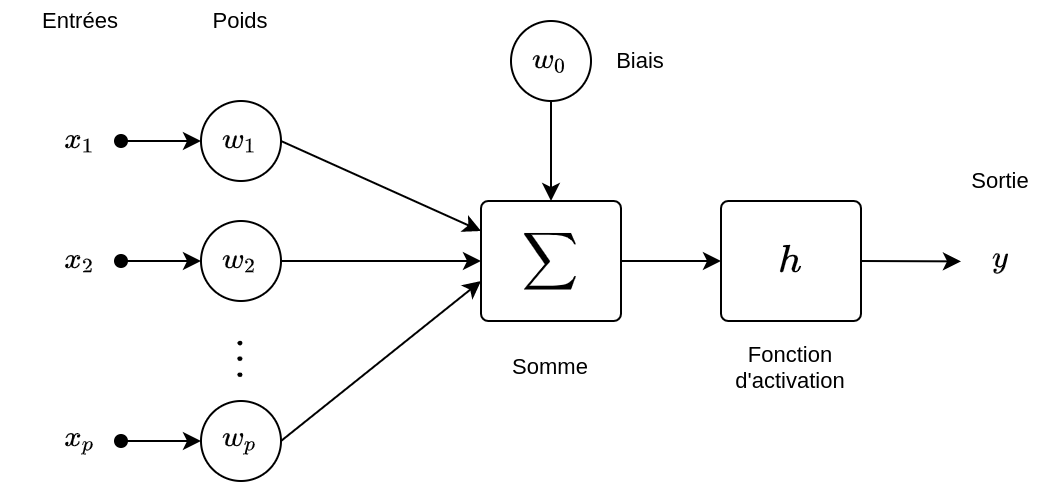
\includegraphics[scale=0.3]{./images/neurone_formel.png}
        \label{img:neurone}
        \caption{Schéma formel d'un neurone}
    \end{figure}

On utilisera aussi une \emph{fonction d'activation} représentée par le seuil $T$. Plus tard, nous utiliserons  des fonctions plus complexes pour donner une valeur de "probabilité" à la sortie d'un neurone. 

\subsection{Apprentissage}

Une fois la structure posée, nous devons définir un algorithme pour apprendre les poids  $(w_1, \dots, w_p)$ dans le but d'avoir une séparation optimale des deux classes dans $\R^p$.  L'idée est donc de faire passer des valeurs $x$ dans le perceptron et d'actualiser les poids  $w_j$ si la prédiction $ \hat{y}$ est différente de la classe $y$.  Une règle simple d'actualisation est de modifier $w_j$ en fonction de la valeur $x_j$ de l'entrée  qu'il pondère. On aura donc la règle suivante : 
    $$ 
        w = 
        \begin{cases}
            w + x \text{ si } y = 1 \text{ et } \hat{y} = -1 \\
            w - x \text{ si } y = - 1 \text{ et } \hat{y} = 1
        \end{cases}
        \quad \iff \quad 
        w = w + y x \text{ si } x \text{ est mal classé}.
    $$

\begin{remark}[Variantes]
    Notre définition de l'actualisation des poids les modifie à chaque itération lors de l'apprentissage. Cela permet une convergence rapide de l'apprentissage, mais peut conduire à une instabilité  si le nombre de poids à traiter est trop grand.  Une solution est donc d'effectuer un \emph{apprentissage par batch}. Cela consiste à faire  passer successivement plusieurs vecteurs $x$, on calcule ensuite l'erreur moyenne commise et on met à jour les poids en fonction de cette erreur moyenne. 
    Un autre possibilité est d'utiliser un \emph{learning rate} $ \nu$ qui bride l'apprentissage. On utilise alors la règle suivante pour actualier $w$ : 
        $$ w = \eta  (y - \hat{y}) x. $$
\end{remark}

Les perceptrons permettent donc de simuler des fonctions booléennes comme illustré ci-dessous : 

% Style mis à jour
\tikzset{
    int/.style={draw, circle, fill=gray!20, minimum size=2.5em, thick},
    input/.style={draw, circle, fill=white!10, minimum size=2em}
}

\begin{figure}[h!]
    \centering
    \begin{minipage}{0.45\textwidth}
        \centering
        \begin{tikzpicture}[auto, >=Stealth, node distance=1.5cm, scale=0.8, transform shape]
        
            % --- NOEUDS ---
            % Le neurone central
            \node [int] (a) {$\Sigma$};

            % Entrées x1 et x2 (positionnées par rapport à 'a')
            \node [input] (x2) [left=1.5cm of a] {$x_2$};
            \node [input] (x1) [above=0.5cm of x2] {$x_1$};
            \node [input] (x3) [below=0.5cm of x2] {$1$};

            % Le Biais arrivant par le haut
            \node (bias_in) [above=1.2cm of a] {$0$};

            % --- FLÈCHES ET POIDS ---
            % Entrées vers neurone avec poids sur les flèches
            \path[->, thick] (x1) edge node[above] {$-1$} (a);
            \path[->, thick] (x2) edge node[above] {$-1$} (a);
            \path[->, thick] (x3) edge node[below] {$-1.5$} (a);
            
            % Flèche du biais
            \path[->, thick] (bias_in) edge (a);

            % Sortie vers la formule
            \node (output) [right=1.0cm of a] {};
            \path[->, thick] (a) edge (output);

            % --- FORMULE À DROITE ---
            \node[right=0cm of output, font=\Large] (formula) {
                $y = x_1 \land x_2$
            };

            % Optionnel : annotation sous la formule pour expliquer la fonction
            % \node[below=0.1cm of formula, font=\small\itshape, text width=4cm, align=center] {
            %     Simule la fonction porte \\ \textbf{NON-ET (NAND)}
            % };
        \end{tikzpicture}
        \captionof{figure}{Fonction AND avec un perceptron}
    \end{minipage}
    \hfill
    \begin{minipage}{0.45\textwidth}
        \centering
        \begin{tikzpicture}[auto, >=Stealth, node distance=1.5cm, scale=0.8, transform shape]
        
            % --- NOEUDS ---
            % Le neurone central
            \node [int] (a) {$\Sigma$};

            % Entrées x1 et x2 (positionnées par rapport à 'a')
            \node [input] (x2) [left=1.5cm of a] {$x_2$};
            \node [input] (x1) [above=0.5cm of x2] {$x_1$};
            \node [input] (x3) [below=0.5cm of x2] {$1$};

            % Le Biais arrivant par le haut
            \node (bias_in) [above=1.2cm of a] {$0$};

            % --- FLÈCHES ET POIDS ---
            % Entrées vers neurone avec poids sur les flèches
            \path[->, thick] (x1) edge node[above] {$-1$} (a);
            \path[->, thick] (x2) edge node[above] {$-1$} (a);
            \path[->, thick] (x3) edge node[below] {$-0.5$} (a);
            
            % Flèche du biais
            \path[->, thick] (bias_in) edge (a);

            % Sortie vers la formule
            \node (output) [right=1.0cm of a] {};
            \path[->, thick] (a) edge (output);

            % --- FORMULE À DROITE ---
            \node[right=0cm of output, font=\Large] (formula) {
                $y = x_1 \lor x_2$
            };

            % Optionnel : annotation sous la formule pour expliquer la fonction
            % \node[below=0.1cm of formula, font=\small\itshape, text width=4cm, align=center] {
            %     Simule la fonction porte \\ \textbf{NON-ET (NAND)}
            % };
        \end{tikzpicture}        
        \captionof{figure}{Fonction OR avec un perceptron}
    \end{minipage}
\end{figure}

Après réflexion, on se rend compte qu'il est impossible de simuler la fonction XOR  avec un seul neurone. Ce sera donc l'objectif des \emph{MLP (Multi Layer Perceptron)}  composés de plusieurs couches de neurones interconnectés. 


\subsection{Perceptron Multi-Couches (MLP)}

Comme énoncé précédemment, le perceptron simple de Rosenblatt présente une limitation fondamentale mise en lumière par Marvin Minsky et Seymour Papert en 1969 : l'impossibilité géométrique de séparer des classes qui ne sont pas linéairement séparables dans l'espace d'entrée $\R^d$, à l'instar de la fonction logique $\mathrm{XOR}$ (ou exclusif).

Pour contourner ce problème, l'approche naturelle consiste à empiler plusieurs couches de neurones formels. Un \emph{Perceptron Multi-Couches} (Multi-Layer Perceptron, noté MLP) est composé :
\begin{enumerate}
    \item D'une couche d'entrée (vecteur $x \in \R^d$) ;
    \item D'une suite de $L \geqslant 1$ \textbf{couches cachées} (hidden layers), qui apprennent des représentations hiérarchiques distribuées ;
    \item D'une couche de sortie produisant la prédiction $\hat{y}$.
\end{enumerate}

\begin{definition}[Formalisation de la passe avant d'un MLP]
    Soit un réseau à $L$ couches cachées. Notons $h^{(0)} = x \in \R^{d_0}$ le vecteur d'entrée. Pour chaque couche $k \in \llbracket 1, L \rrbracket$ de dimension $d_k$, le vecteur d'activation est régi par les relations de récurrence :
    \begin{align}
        a^{(k)} &= W^{(k)} h^{(k-1)} + b^{(k)} \in \R^{d_k} \quad &\text{(pré-activation)} \\
        h^{(k)} &= g^{(k)}\left(a^{(k)}\right) \in \R^{d_k} \quad &\text{(activation)}
    \end{align}
    où $W^{(k)} \in \R^{d_k \times d_{k-1}}$ désigne la matrice de poids de la couche $k$, $b^{(k)} \in \R^{d_k}$ le vecteur de biais associé, et $g^{(k)} : \R \to \R$ une fonction d'activation non linéaire appliquée composante par composante.
    Pour la couche de sortie $k = L+1$, on applique une fonction terminale $o$ :
    \begin{equation}
        \hat{y} = h^{(L+1)} = o\left(W^{(L+1)} h^{(L)} + b^{(L+1)}\right).
    \end{equation}
\end{definition}

\begin{remark}[Interprétation géométrique des frontières de décision]
    Chaque neurone d'une première couche cachée partitionne l'espace $\R^d$ par un demi-espace délimité par un hyperplan affine. Les neurones de la deuxième couche cachée effectuent une intersection booléenne (opérateur $\mathrm{ET}$) de ces demi-espaces, formant ainsi des polyèdres convexes. Enfin, les couches suivantes peuvent réaliser l'union (opérateur $\mathrm{OU}$) de régions convexes disjointes, rendant le réseau théoriquement capable d'approximer n'importe quelle frontière de décision fermée ou ouverte arbitrairement complexe.
\end{remark}

% =============================================================================
% Fonctions d'activation et Classification linéaire multiclasse

\section{Fonctions d'Activation et Classification Multiclasse}

\subsection{Fonctions d'activation usuelles}

Le choix d'une fonction d'activation non linéaire $g$ est indispensable : sans elle, la composition successive d'opérations affines $W^{(L)}(\dots (W^{(1)}x + b^{(1)}) \dots) + b^{(L)}$ resterait strictement équivalente à une unique transformation affine globale $\tilde{W}x + \tilde{b}$, ruinant tout l'intérêt de la profondeur.

\begin{definition}[Fonctions d'activation courantes]
    On définit ainsi différentes fonctions d'activations communément utilisées en sortie d'un neuronne. Pour tout réel $z \in \R$ on a :
    \begin{itemize}
        \item \textbf{Sigmoïde (logistique)} : 
        \begin{equation}
            \sigma(z) = \frac{1}{1 + e^{-z}}. 
        \end{equation}
        Elle projette $\R$ sur $]0, 1[$ et vérifie l'identité remarquable $\sigma'(z) = \sigma(z)(1 - \sigma(z))$.
        \item \textbf{Tangente hyperbolique} : 
        \begin{equation}
            \tanh(z) = \frac{e^z - e^{-z}}{e^z + e^{-z}} \in ]-1, 1[, 
        \end{equation}
        centrée en zéro, de dérivée $\tanh'(z) = 1 - \tanh^2(z)$.
        \item \textbf{Rectified Linear Unit (ReLU)} : 
        \begin{equation}
            g(z) = \max(0, z).
        \end{equation}
        Sa dérivée vaut $1$ pour $z > 0$ et $0$ pour $z < 0$. Elle évite la saturation des gradients pour des entrées positives.
        \item \textbf{Leaky ReLU} : pour $\alpha \in ]0, 1[$ (couramment $\alpha = 0{,}01$), $g(z) = \max(\alpha z, z)$. Elle évite le problème des "neurones morts" lorsque $z < 0$.
        \item \textbf{Softplus} : 
        \begin{equation}
            g(z) = \log(1 + e^z),
        \end{equation}
        approximation analytique différentiable de la ReLU.
    \end{itemize}
\end{definition}

\subsection{Classification multiclasse et fonction Softmax}

Considérons un problème de classification à $K > 2$ classes mutuellement exclusives. La couche finale produit un vecteur de scores réels non normalisés $a = W^{(L+1)}h^{(L)} + b^{(L+1)} \in \R^K$, appelés \emph{logits}.

\begin{definition}[Opérateur Softmax]
    L'opérateur Softmax normalise un vecteur de logits $a = (a_1, \dots, a_K)^\top$ en une distribution discrète de probabilités $p = (p_1, \dots, p_K)^\top \in [0, 1]^K$ définie par :
    \begin{equation}
        \forall c \in \llbracket 1, K \rrbracket, \quad p_c = \operatorname{Softmax}(a)_c = \frac{e^{a_c}}{\sum_{j=1}^{K} e^{a_j}}.
    \end{equation}
    On a immédiatement $\forall c, \; p_c > 0$ et $\sum_{c=1}^K p_c = 1$. La classe prédite est $\hat{y} = \arg\max_{c} p_c$.
\end{definition}

% =============================================================================
% Fonctions de perte

\section{Fonctions de Perte (\emph{Loss Functions})}

En apprentissage supervisé, puisque nous connaissons les \emph{labels} associés à chaque prédiction, nous sommes capables d'évaluer le modèle en temps réel sur chacune de ses prédiction sur les données d'entraînement. Ainsi, l'évaluation de la discordance entre la cible réelle $y$ et la sortie estimée $\hat{y}$ s'effectue au moyen d'une fonction de coût différentiable $\mathcal{L}(y, \hat{y})$ que l'on appellera \emph{fonction de perte} ou \emph{loss}. 

\subsection{Entropie croisée binaire (BCE)}

\begin{remark}[Limites de la MSE]
    Pour une classification binaire avec $y \in \{0, 1\}$ et une prédiction de probabilité $\hat{y} = \sigma(z) \in ]0, 1[$, l'erreur quadratique usuelle MSE s'avère sous-optimale du fait de zones de saturation où le gradient s'annule pour des erreurs maximales. On introduit la perte d'entropie croisée binaire.    
\end{remark}

\begin{definition}[Binary Cross-Entropy]
    Pour $y \in \{0, 1\}$ et $\hat{y} \in ]0, 1[$ :
    \begin{equation}
        \mathcal{L}_{\mathrm{BCE}}(y, \hat{y}) = - y \log(\hat{y}) - (1 - y) \log(1 - \hat{y}).
    \end{equation}
\end{definition}

\begin{proposition}[Stabilité numérique de la BCE]
    En injectant l'activation logistique $\hat{y} = \sigma(z) = \frac{1}{1 + e^{-z}}$ directement dans la perte, on évite les dépassements de capacité flottante (\emph{overflow}) via l'expression analytique exacte :
    \begin{equation}
        \mathcal{L}_{\mathrm{BCE}}(y, \sigma(z)) = \max(z, 0) - z \cdot y + \log\left(1 + e^{-|z|}\right).
    \end{equation}
\end{proposition}

% TODO : Ajouter d'autres fonctions de perte


% =============================================================================
% Rétropropagation et Dérivation Automatique

\section{Rétropropagation du Gradient et Dérivation Automatique}

Comme vu au début de ce chapitre, l'apprentissage se fait par une recherche des "meilleurs" poids possibles pour le modèle dans l'objectif de minimiser l'erreur commise. Maintenant que nous avons introduit la fonciton de perte \emph{loss}, nous cherchons donc à faire une minimisation de cette fonction \emph{loss}. 

La principale problématique dans ce processus est le calcul de son \emph{gradient}. En effet, pour trouver des candidats minimiseurs, la condition d'optimalité d'ordre 1 nous demande d'annuler ce gradient. Nous devons donc être capable de calculer les dérivées partielles de la \emph{loss} en fonction des poids du modèle. On utilise pour cela l'algorithme de \emph{rétropropagation} à l'aide de \emph{graphes computationnels}. 

\subsection{Rétropropagation sur un neurone formel}

Considérons un unique neurone formel doté d'une entrée $x \in \R^d$, d'une pré-activation $a = w^\top x + b$, d'une activation $\hat{y} = \sigma(a)$, et d'une perte quadratique $\mathcal{L} = \frac{1}{2}(y - \hat{y})^2$. Par application directe de la règle de dérivation en chaîne (\emph{Chain Rule}) :
\begin{equation}
    \frac{\partial \mathcal{L}}{\partial w_i} = \frac{\partial \mathcal{L}}{\partial \hat{y}} \cdot \frac{d\hat{y}}{da} \cdot \frac{\partial a}{\partial w_i} = - (y - \hat{y}) \cdot \hat{y}(1 - \hat{y}) \cdot x_i.
\end{equation}
On retrouve le terme d'erreur $(y - \hat{y})$, pondéré par la pente de la sigmoïde $\hat{y}(1 - \hat{y})$ et la projection d'entrée $x_i$. Si l'on remplace la perte quadratique par la $\mathcal{L}_{\mathrm{BCE}}$, le terme $\hat{y}(1-\hat{y})$ se simplifie élégamment au dénominateur :
\begin{equation}
    \frac{\partial \mathcal{L}_{\mathrm{BCE}}}{\partial a} = \hat{y} - y \implies \frac{\partial \mathcal{L}_{\mathrm{BCE}}}{\partial w} = (\hat{y} - y)x.
\end{equation}

\subsection{Rétropropagation dans un MLP (\emph{Backpropagation})}

% TODO : Rajouter partie graphe computationnel et exemple de calcul à la main

Dans un graphe multicouches, les erreurs locales sont propagées de l'aval vers l'amont :
\begin{definition}[Rétropropagation multicouche]
    Posons $\delta^{(k)} = \frac{\partial \mathcal{L}}{\partial a^{(k)}}$ le vecteur de sensibilité de la couche $k$.
    \begin{align}
        \text{Couche de sortie } (L+1) : \quad \delta^{(L+1)} &= \nabla_{a^{(L+1)}} \mathcal{L} \\
        \text{Couches cachées } (k = L, \dots, 1) : \quad \delta^{(k)} &= \left( (W^{(k+1)})^\top \delta^{(k+1)} \right) \odot g'^{(k)}\left(a^{(k)}\right)
    \end{align}
    où $\odot$ désigne le produit d'Hadamard (terme à terme). Les gradients s'en déduisent immédiatement :
    \begin{equation}
        \frac{\partial \mathcal{L}}{\partial W^{(k)}} = \delta^{(k)} \left(h^{(k-1)}\right)^\top \in \R^{d_k \times d_{k-1}}, \qquad \frac{\partial \mathcal{L}}{\partial b^{(k)}} = \delta^{(k)} \in \R^{d_k}.
    \end{equation}
\end{definition}

\subsection{Graphes de calcul et implémentation PyTorch}

En pratique, le calcul symbolique manuel des dérivées est remplacé par l'auto-différenciation en mode inverse (\emph{reverse-mode automatic differentiation}) matérialisée par un graphe acyclique orienté (DAG). 

\begin{lstlisting}[language=Python, caption={Implémentation d'un MLP complet sous PyTorch}]
import torch
import torch.nn as nn

class MultiLayerPerceptron(nn.Module):
    def __init__(self, in_features: int, hidden_dim: int, out_classes: int):
        super(MultiLayerPerceptron, self).__init__()
        self.network = nn.Sequential(
            nn.Linear(in_features, hidden_dim),
            nn.ReLU(),
            nn.Linear(hidden_dim, hidden_dim),
            nn.ReLU(),
            nn.Linear(hidden_dim, out_classes)
        )
        
    def forward(self, x: torch.Tensor) -> torch.Tensor:
        # Retourne les logits bruts (non normalises)
        return self.network(x)

# Instanciation et passe avant/arriere
model = MultiLayerPerceptron(in_features=784, hidden_dim=128, out_classes=10)
criterion = nn.CrossEntropyLoss() # Integre log-softmax et NLL
optimizer = torch.optim.SGD(model.parameters(), lr=0.01, momentum=0.9)

x_dummy = torch.randn(32, 784) # Batch de 32 observations
y_target = torch.randint(0, 10, (32,))

optimizer.zero_grad()
logits = model(x_dummy)
loss = criterion(logits, y_target)
loss.backward() # Calcul automatique des gradients via Autograd
optimizer.step()
\end{lstlisting}

\subsection{Optimisation par descente de gradient avec inertie (Momentum)}

La descente de gradient stochastique standard (SGD) présente de fortes oscillations transverses dans les vallées mal conditionnées (matrice hessienne à fort conditionnement). La méthode avec moment régularise la trajectoire en accumulant une moyenne exponentielle glissante des vitesses passées :
\begin{align}
    v_t &= \beta v_{t-1} + \alpha \nabla_W \mathcal{L}_t \quad \text{avec } \beta \in [0, 1[ \\
    W_{t+1} &= W_t - v_t
\end{align}
où $\alpha > 0$ représente le pas d'apprentissage (\emph{learning rate}).

% TODO : Rajouter autres params et optimiseurs



\part[]{Mathématiques du Machine Learning}
\setcounter{chapter}{0}
% ==================================================================================================================================
% Mathématiques du Machine Learning

% - - - - - - - - - - - - - - - - - - - - - - - - - 
%                       TITLE
% - - - - - - - - - - - - - - - - - - - - - - - - - 


% - - - - - - - - - - - - - - - - - - - - - - - - - 
%               Chapters Inclusion
% - - - - - - - - - - - - - - - - - - - - - - - - - 

\chapter{Introduction à l'Apprentissage Supervisé}
% ========================================================================================================
% Introduction 

\minitoc 

L'objectif de ce cours est de formaliser le processus d'apprentissage d'un modèle dans le cas d'un apprentissage supervisé. On commencera par définit ce qu'est ce type d'apprentissage puis ce que l'on entend par "apprendre". Différentes métriques seront introduites pour le quantifier. 

% ======================================================================
% Des données et des prédictions

\section{Des données et des prédictions}

L'ensemble du processus d'apprentissage s'appuie sur les concepts de \emph{données} et de \emph{prédictions}. 

\begin{definition}[Observations]
    Formellement, on définira les \emph{données} d'un problème de machine learning par un ensemble de couples $(x,y) \in \mathcal{X} \times \mathcal{Y}$ que l'on appellera \emph{données d'entraînement} ou \emph{observations}. On notera cet ensemble $D$ qui contiendra $N$ couples. 
\end{definition}

Ces entrées et sorties attendues peuvent être de différents types en fonction du problème considéré. Les entrées peuvent être des images, des vidéos, du son ou un texte. On les modélisera en général par des vecteurs de $\R^d$ lorsque c'est possible. On appellera donc $d \in \N$ la dimension des données à l'entrée du modèle. 

Les sorties peuvent être de deux types différents en apprentissage supervisé :
\begin{itemize}
    \item Un ensemble d'entiers $\{1, \dots, k\}$. On parlera alors de problème de \emph{classification}. 
    \item Un vecteur de $\R^{d'}$. On parlera alors d'un problème de \emph{régression}. 
\end{itemize}

% \begin{example}
%     \begin{itemize}
%         \item Un laboratoire en médecine cherche à développer un modèle permettant de prédire si un patient est sujet à développer une maladie rare. Pour cela, il dispose de l'ensemble de ses données médicales et d'un jeu de données composé des données médicales et du résultat 
%     \end{itemize}
% \end{example}

L'objectif est d'être capable, à partir d'une nouvelle donnée $x \in \mathcal{X}$ d'inférer/prédire le $y$ qui lui correspond le mieux. Plus formellement, on cherche à \emph{apprendre} une fonction $f$ à partir des données d'entraînement telle que : 
\begin{equation}
    y \simeq f(x)
\end{equation}

% ======================================================================
% Formalisation Mathématique

\section{Formalisation mathématique}

Pour apprendre une telle fonction, nous devons admettre différentes hypothèses sur le jeu de données de départ $D$. La première est que ce jeu de données suit une certaine loi de probabilité $ \myP$. La seconde est que chaque échantillon $(x_i, y_i), i \in \llbracket 1, N \rrbracket$ est indépendant des autres ($D$ est un ensemble de réalisation i.i.d de la loi $ \myP$). 

\subsection{Fonction de Perte}

Pour effectuer cet apprentissage, nous devons être capable de savoir à quel point notre modèle se trompe sur une prédiction donnée par rapport à la vraie valeur issue du jeu de données. Nous définissons pour cela une \emph{fonction de perte}. 

\begin{definition}[Fonction de perte]
    La \emph{fonction de perte}, notée $l$, calcule l'erreur induite par la prédiction de $z \in \mathcal{Y}$ alors que la valeur attendue était $y \in \mathcal{Y}$ pour une entrée $x \in \mathcal{x}$. Elle vérifie donc : 
    \begin{equation}
        l : \mathcal{Y} \times \mathcal{Y} \longrightarrow \R.
    \end{equation}
\end{definition}

\begin{example}
    Dans le cas d'une classification binaire (i.e $ \mathcal{Y} = \{0, 1\}$), on peut simplement utiliser la \emph{Zero/One Loss} définie par $l(y, z) = \mathbbm{1}_{z \not = y}$. 

    Dans le cas de la régression, on utilisera plutôt les $L^1$ Loss ou $L^2$ Loss définies par : 
    $$ l(y, z) = \|y - z\|^2, \quad \text{et} \quad l(y, z) = \|y - z\|$$ 
\end{example}

\subsection{Les Risques}

Ces différentes fonctions de pertes, aussi bien définies soient-elles, ne nous donnent d'un apperçu des erreurs du modèle en temps réel. Nous avons aussi desoin d'avoir une idée plus fine des performances du modèle vis-à-vis de la distribution de probabilité $\myP$ du jeu de données $D$. 
On définit pour cela les \emph{risques}. 

\begin{definition}[Risque Moyen]
    On définit le \emph{risque moyen}, noté $ \mathcal{R}(f)$, d'une fonction $f$ sur l'espace $ \mathcal{X} \times \mathcal{Y}$ par l'espérance de la perte du ce même jeu de données. 
    \begin{equation}
        \boxed{\mathcal{R}(f) := \int_{ \mathcal{X} \times \mathcal{Y}} l(y, f(x)) \; dp(x, y) \; dx \; dy = \mathbb{E} \left(l(y, f(x))\right)}
    \end{equation}
    où $p$ est le densité de la probabilité $ \myP$. 
\end{definition}

\begin{example}
    Dans le cas de la classification binaire, le risque moyen se simplfie facilement : 
    \begin{align*}
        \mathcal{R}(f) &= \int_{ \mathcal{X} \times \mathcal{Y}} \mathbbm{1}_{y \not = f(x)} \; d \myP(x,y) \\ 
        &= 0 \times \myP(f(x) = y) + 1 \times \myP(f(x) \not = y) \\ 
        &= \myP(f(x) \not = y)
    \end{align*}
\end{example}

À noter que ce risque est calculé sur l'espace entier des données possibles. En pratique, si celui-ci est infini, il est incalculable. On préférera donc utiliser le \emph{risque empirique}. 

\begin{definition}[Risque Empirique]
    Le risque empirique, noté $ \hat{\mathcal{R}}(f)$ est donné par la moyenne empirique des pertes sur un jeu de données $ D$. 
    \begin{equation}
        \boxed{\hat{ \mathcal{R}}(f) := \frac{1}{N} \sum_{i=1}^{N} l(y_i, f(x_i)).}
    \end{equation}
\end{definition}

\begin{proposition}[Convergance]
    Grâce aux hypothèses précédentes, on peut invoquer des théorèmes de convergence sur les suites de variables aléatoires pour caractériser la limite de ce risque empirique. 

    Ainsi, si $ f \in L^1$ alors, d'après la \emph{Loi Forte des Grands Nombres}, on a que : 
    \begin{equation}
        \hat{ \mathcal{R}}(f) \underset{n \to \infty}{\overset{\text{p.s}}{\longrightarrow}} \mathcal{R}(f).
    \end{equation}
    Si, de plus $f \in L^2$, alors on a une idée de la vitesse de convergence de ce risque empirique : 
    \begin{equation}
        \sqrt{n}(\hat{ \mathcal{R}}(f) - \mathcal{R}(f)) \underset{n \to \infty}{\overset{\text{Loi}}{\longrightarrow}} \mathcal{N}(0, \V(l(y, f(x)))).
    \end{equation}
\end{proposition}

En pratique, pour toute fonction apprise $f$, on aura $ \hat{ \mathcal{R}}(f) \simeq \mathcal{R}(f)$. 

% ======================================================================
% Risque et prédicteur de Bayes

\section{Risque et prédicteur de Bayes}

L'objectif théorique de l'apprentissage statistique est de trouver une fonction $f$ qui minimise le risque moyen $\mathcal{R}(f)$ parmi l'ensemble $\mathcal{F}_{\text{all}}$ de toutes les fonctions mesurables de $\mathcal{X}$ dans $\mathcal{Y}$. 

\begin{definition}[Prédicteur et Risque de Bayes]
    On appelle \emph{prédicteur de Bayes}, noté $f^*$, la fonction optimale (si elle existe) qui minimise le risque moyen sur l'espace de toutes les fonctions mesurables :
    \begin{equation}
        \boxed{f^* \in \arg \min_{f \in \mathcal{F}_{\text{all}}} \mathcal{R}(f)}
    \end{equation}
    Le risque associé, noté $\mathcal{R}^* = \mathcal{R}(f^*)$, est appelé le \emph{risque de Bayes} (ou erreur irréductible). Pour toute fonction mesurable $f$, on a trivialement :
    \begin{equation}
        \mathcal{R}(f) \geqslant \mathcal{R}^*
    \end{equation}
\end{definition}

Pour calculer explicitement $f^*$, on utilise la loi des espérances itérées (conditionnement par rapport à $X$) :
\begin{equation}
    \mathcal{R}(f) = \mathbb{E}_{(X, Y)}\left[ l(Y, f(X)) \right] = \mathbb{E}_X \left[ \mathbb{E}_{Y|X} \left[ l(Y, f(X)) \mid X \right] \right]
\end{equation}
Minimiser $\mathcal{R}(f)$ revient donc à minimiser l'espérance conditionnelle point par point pour chaque $x \in \mathcal{X}$ :
\begin{equation}
    f^*(x) \in \arg \min_{z \in \mathcal{Y}} \mathbb{E}_{Y|X=x}\left[ l(Y, z) \mid X = x \right]
\end{equation}

\subsection{Forme explicite selon la tâche}

\begin{proposition}[Cas de la régression quadratique ($L^2$)]
    Pour la perte quadratique $l(y, z) = (y - z)^2$, le prédicteur de Bayes est l'espérance conditionnelle de $Y$ sachant $X$ :
    \begin{equation}
        \boxed{f^*(x) = \mathbb{E}[Y \mid X = x]}
    \end{equation}
\end{proposition}

\begin{proof}
    Fixons $x \in \mathcal{X}$. On cherche $z \in \R$ minimisant $\phi(z) = \mathbb{E}\left[(Y - z)^2 \mid X = x\right]$.
    \begin{align*}
        \phi(z) &= \mathbb{E}\left[Y^2 \mid X = x\right] - 2z \mathbb{E}\left[Y \mid X = x\right] + z^2
    \end{align*}
    $\phi$ est une fonction convexe et dérivable en $z$. En annulant la dérivée :
    $$\phi'(z) = -2\mathbb{E}[Y \mid X = x] + 2z = 0 \iff z = \mathbb{E}[Y \mid X = x]$$
\end{proof}

\begin{proposition}[Cas de la classification binaire (perte 0/1)]
    Pour $\mathcal{Y} = \{0, 1\}$ et la perte 0/1 $l(y, z) = \mathbbm{1}_{y \neq z}$, le prédicteur de Bayes attribue la classe la plus probable a posteriori :
    \begin{equation}
        \boxed{f^*(x) = \mathbbm{1}_{\myP(Y = 1 \mid X = x) \ge 1/2}}
    \end{equation}
\end{proposition}

\begin{proof}
    Pour un $x \in \mathcal{X}$ donné et pour $z \in \{0, 1\}$ :
    \begin{align*}
        \mathbb{E}\left[\mathbbm{1}_{Y \neq z} \mid X = x\right] &= \myP(Y \neq z \mid X = x) \\
        &= 1 - \myP(Y = z \mid X = x)
    \end{align*}
    Minimiser cette quantité revient à maximiser $\myP(Y = z \mid X = x)$, ce qui donne la règle du maximum a posteriori (MAP).
\end{proof}

\chapter{Régression Linéaire et Régression Ridge}
% ===============================================================================
% Introduction 

\minitoc 

On pose ici le contexte d'une \emph{régression linéaire}. On cherche donc à apprendre une fonction pour décrire un jeu de données $(x_1, y_1), \dots, (x_n, y_n) \in \mathcal{X} \times \mathcal{Y}$. Dans le cas du modèle linéaire, on fera l'hypothèse forte suivante : 
\begin{equation}
    (H) : f_\theta = \varphi(x)^t \theta, \quad \theta \in \R^d.
\end{equation} 
Pour construire cette fonction, on utilisera l'estimateur du risque empirique (ERM) définit par : 
\begin{equation}
    \hat{R}( \theta) \in \underset{ \theta \in \Theta}{\arg \min} \frac{1}{n} \sum_{i=1}^{n} \left(y_i - f_\theta(x_i)\right)^2. 
\end{equation}

\begin{example}
    La forme de l'application $ \varphi$ caractérisera la \emph{feature map} (i.e l'ensemble des fonctions possibles pour interpoler le nuage de points). 
    \begin{itemize}
        \item si $ \varphi(x) = x$, alors on aura une estimation linéaire en $x$, 
        \item si $ \varphi(x) = \begin{pmatrix} x \\ 1 \end{pmatrix}$ alors l'estimation sera \emph{affine} en $x$, 
        \item si $ \varphi(x) \in \R^d[x]$, alors l'estimation sera \emph{polynômiale} en $x$. On pourra aller jusqu'au degré $d$ pour utiliser des polynômes de Lagrange. 
    \end{itemize}
\end{example}

\begin{notation}
    On notera $y = \begin{pmatrix} y_1 \\ \dots \\ y_n \end{pmatrix}$ le vecteur des étiquettes du jeu de données et $ \Phi = \begin{pmatrix} \varphi(x_1)^t \\ \dots \\ \varphi(x_n)^t\end{pmatrix} \in \R^{n \times d}$ la matrice contenant toutes les prédictions données par la \emph{feature map}. 
    On aura donc : $ \hat{R}(\theta) = \frac{1}{n} \| y - \Phi \theta \|_2^2$. 
\end{notation}

% =======================================================
% Moindres Carrés 

\section{Moindres Carrés}

Nous sommes en présence d'un problème de régression. Grâces aux notations matricielles précédement posées, nous sommes capable de calculer une solution explicite à la main. 

On cherche à calculer explicitement $\hat{\theta} \in \arg \min_{\theta \in \R^d} \hat{R}(\theta)$. Pour cela, on utilise la condition nécessaire d'optimalité d'ordre 1 : $\nabla_\theta \hat{R}(\hat{\theta}) = 0$. Commençons donc par calculer le gradient : 
\begin{equation}
    \hat{R}(\theta) = \frac{1}{n} \| y - \Phi \theta \|_2^2
\end{equation}
\begin{equation}
    \nabla_\theta \hat{R}(\theta) = \frac{2}{n} \Phi^\top (\Phi \theta - y)
\end{equation}

En résolvant l'équation $\nabla_\theta \hat{R}(\hat{\theta}) = 0$, on obtient les \emph{équations normales} :
\begin{equation}
    (*) : \Phi^\top \Phi \hat{\theta} = \Phi^\top y
\end{equation}

En supposant que $\Phi$ est de rang plein ($rg(\Phi) = d$, soit des colonnes linéairement indépendantes), la matrice de Gram $\Phi^\top \Phi \in \R^{d \times d}$ est inversible, ce qui donne :
\begin{equation}
    (*) \iff \boxed{\hat{\theta} = \left( \Phi^\top \Phi\right)^{-1} \Phi^\top y}
\end{equation}

La fonction $\hat{R}$ étant convexe, ce point stationnaire est un minimum global.
On calcule ainsi explicitement l'estimateur des moindres carrés (OLS), qui fournit le prédicteur linéaire optimal sur l'échantillon d'entraînement.

\begin{proposition}
    Géométriquement, les prédictions $\hat{y} = \Phi \hat{\theta}$ correspondent à la projection orthogonale du vecteur d'observations $y \in \R^n$ sur le sous-espace vectoriel $\operatorname{Im}(\Phi) \subset \R^n$ engendré par les colonnes de $\Phi$ :
    \begin{equation}
        \hat{\theta} \in \underset{\theta \in \R^d}{\arg \min} \; \frac{1}{n} \left\| y - \Phi \theta \right\|_2^2 \quad
        \iff \quad \hat{y} \in \underset{z \in \operatorname{Im}(\Phi)}{\arg \min} \; \frac{1}{n} \left\| y - z \right\|_2^2
    \end{equation}
\end{proposition}

\begin{figure}[htbp]
    \centering
    \begin{tikzpicture}[
        x={(1cm, 0cm)}, 
        y={(0.6cm, 0.35cm)}, 
        z={(0cm, 1cm)}, 
        scale=1.2, 
        >=latex
    ]
        % --- Coordonnées des points ---
        \coordinate (O)  at (0, 0, 0);           % Origine
        \coordinate (Yh) at (2.2, 1.8, 0);       % Projection orthogonale \hat{y}
        \coordinate (Y)  at (2.2, 1.8, 2.5);     % Point y au-dessus du plan

        % --- Plan horizontal : \mathrm{Im}(\phi) ---
        \filldraw[fill=blue!5, draw=blue!40, thick] 
            (-1.5, -1.0, 0) -- (4.2, -1.0, 0) -- (4.2, 3.5, 0) -- (-1.5, 3.5, 0) -- cycle;

        % Label du sous-espace / plan
        \node[blue!70!black, anchor=north east] at (4.0, 3.3, 0) {$\operatorname{Im}(\phi)$};

        % --- Vecteur projeté de O vers \hat{y} ---
        \draw[->, very thick, teal] (O) -- (Yh) 
            node[midway, below right, text=teal] {$\hat{y} = \Pi_{\operatorname{Im}(\phi)}(y)$};

        % --- Ligne de projection orthogonale (y vers \hat{y}) ---
        \draw[dashed, thick, red!70!black] (Y) -- (Yh);

        % --- Symbole de l'angle droit en 3D au niveau de \hat{y} ---
        % Construit à l'aide des directions vers O et vers Y
        \draw[thick, gray!70!black] 
            ($(Yh)!0.3cm!(O)$) -- 
            ($($(Yh)!0.3cm!(O)$) + (0, 0, 0.3)$) -- 
            ($(Yh) + (0, 0, 0.3)$);

        % --- Vecteur reliant l'origine à y ---
        \draw[->, thick, purple!80!black] (O) -- (Y) 
            node[midway, left=2pt] {$y$};

        % --- Vecteur résidu / erreur (de \hat{y} vers y) ---
        \draw[->, thick, dashed, red!80!black] (Yh) -- (Y) 
            node[midway, right] {$y - \hat{y}$};

        % --- Points (marquage) ---
        \filldraw[black] (O) circle (1.5pt) node[below left] {$O$};
        \filldraw[red!70!black] (Yh) circle (1.5pt) node[below right] {$\hat{y}$};
        \filldraw[purple!80!black] (Y) circle (1.5pt) node[above] {$y$};

    \end{tikzpicture}
    \caption{Projection orthogonale du vecteur d'observations $y$ sur le sous-espace affine $\operatorname{Im}(\phi)$ et décomposition de l'erreur résiduelle $y - \hat{y} \perp \operatorname{Im}(\phi)$.}
    \label{fig:projection_orthogonale_phi}
\end{figure}


% =======================================================
% Analyse statistique -- design fixe

\section{Analyse statistique -- design fixe}

Dans cette section, on se place sous l'hypothèse du \emph{design fixe} : les points $x_i \in \mathcal{X}$ (et donc la matrice $\Phi \in \R^{n \times d}$) sont déterministes et fixés. Seules les étiquettes $y_i$ sont aléatoires.

\begin{definition}[Modèle à design fixe]
    Le modèle probabiliste d'observation s'écrit :
    \begin{enumerate}
        \item $y = \Phi \theta_* + \varepsilon$, avec $\theta_* \in \R^d$ le paramètre vrai inconnu.
        \item Le vecteur de bruit $\varepsilon = (\varepsilon_1, \dots, \varepsilon_n)^\top \in \R^n$ vérifie $\mathbb{E}(\varepsilon) = 0$ et $\operatorname{Var}(\varepsilon) = \mathbb{E}(\varepsilon \varepsilon^\top) = \sigma^2 I_n$.
    \end{enumerate}
    Le risque moyen sous design fixe est défini par :
    \begin{equation}
        R(\theta) = \frac{1}{n} \mathbb{E}_y \left[ \left\| y - \Phi \theta \right\|_2^2 \right].
    \end{equation}
\end{definition}

On introduit la matrice de covariance empirique $\hat{\Sigma} := \displaystyle \frac{1}{n} \Phi^\top \Phi \in \R^{d \times d}$, associée à la semi-norme $\|u\|_{\hat{\Sigma}}^2 := u^\top \hat{\Sigma} u = \displaystyle \frac{1}{n} \|\Phi u\|_2^2$.

\begin{proposition}[Décomposition Biais-Variance]
    Pour tout vecteur fixe $\theta \in \R^d$ :
    \begin{align*}
        R(\theta) &= \frac{1}{n} \mathbb{E}_\varepsilon \left[ \left\| \Phi (\theta_* - \theta) + \varepsilon \right\|_2^2 \right] \\
        &= \frac{1}{n} \|\Phi (\theta_* - \theta)\|_2^2 + \frac{1}{n} \mathbb{E}\left[\|\varepsilon\|_2^2\right] + \frac{2}{n} (\theta_* - \theta)^\top \Phi^\top \mathbb{E}[\varepsilon] \\
        &= \|\theta - \theta_*\|_{\hat{\Sigma}}^2 + \sigma^2.
    \end{align*}

    % TODO : Ajouter calcul risque de Bayes + le calculer à la main
    
    Le risque de Bayes est atteint en $\theta_*$ : $R^* = R(\theta_*) = \sigma^2$. Par conséquent, pour un estimateur aléatoire $\hat{\theta}$ dépendant de $y$ (donc de $\varepsilon$) :
    \begin{equation}
        \boxed{\mathbb{E}_{\hat{\theta}}\left[ R(\hat{\theta}) \right] - R^* = \underbrace{\left\| \mathbb{E}(\hat{\theta}) - \theta_* \right\|_{\hat{\Sigma}}^2}_{\text{Biais}^2} + \underbrace{\mathbb{E}_{\hat{\theta}}\left[ \left\| \hat{\theta} - \mathbb{E}(\hat{\theta}) \right\|_{\hat{\Sigma}}^2 \right]}_{\text{Variance}}}
    \end{equation}
\end{proposition}

\begin{theorem}[Biais et Variance des Moindres Carrés]
    Dans le cas de l'estimateur des moindres carrés $\hat{\theta} = (\Phi^\top \Phi)^{-1} \Phi^\top y$ :
    \begin{equation}
        \text{Biais}^2 = 0 \quad \text{et} \quad \mathbb{E}\left[ R(\hat{\theta}) \right] - R^* = \frac{\sigma^2 d}{n}.
    \end{equation}
\end{theorem}

\begin{proof}
    \begin{itemize}
        \item \emph{Calcul du biais} : 
        \begin{align*}
            \mathbb{E}(\hat{\theta}) &= \mathbb{E}\left[ (\Phi^\top \Phi)^{-1} \Phi^\top (\Phi \theta_* + \varepsilon) \right] \\
            &= \theta_* + (\Phi^\top \Phi)^{-1} \Phi^\top \mathbb{E}[\varepsilon] = \theta_*.
        \end{align*}
        L'estimateur est sans biais, d'où $\text{Biais}^2 = 0$.

        \item \emph{Calcul de la variance} : On exprime la variance sous forme de trace :
        \begin{align*}
            \text{Variance} &= \mathbb{E}\left[ (\hat{\theta} - \theta_*)^\top \hat{\Sigma} (\hat{\theta} - \theta_*) \right] \\
            &= \mathbb{E}\left[ \operatorname{tr}\left( \hat{\Sigma} (\hat{\theta} - \theta_*) (\hat{\theta} - \theta_*)^\top \right) \right] \\
            &= \operatorname{tr}\left( \hat{\Sigma} \, \mathbb{E}\left[ (\hat{\theta} - \theta_*) (\hat{\theta} - \theta_*)^\top \right] \right).
        \end{align*}
        Or, $\hat{\theta} - \theta_* = (\Phi^\top \Phi)^{-1} \Phi^\top \varepsilon$, donc :
        \begin{align*}
            \mathbb{E}\left[ (\hat{\theta} - \theta_*) (\hat{\theta} - \theta_*)^\top \right] &= (\Phi^\top \Phi)^{-1} \Phi^\top \mathbb{E}[\varepsilon \varepsilon^\top] \Phi (\Phi^\top \Phi)^{-1} \\
            &= \sigma^2 (\Phi^\top \Phi)^{-1} \Phi^\top I_n \Phi (\Phi^\top \Phi)^{-1} \\
            &= \sigma^2 (\Phi^\top \Phi)^{-1} = \frac{\sigma^2}{n} \hat{\Sigma}^{-1}.
        \end{align*}
        En réinjectant dans l'expression de la trace :
        \begin{align*}
            \text{Variance} &= \operatorname{tr}\left( \hat{\Sigma} \cdot \frac{\sigma^2}{n} \hat{\Sigma}^{-1} \right) = \frac{\sigma^2}{n} \operatorname{tr}(I_d) = \frac{\sigma^2 d}{n}.
        \end{align*}
    \end{itemize}
\end{proof}

% =======================================================
% Régression Ridge -- design fixe

\section{Régression Ridge -- design fixe}

Dans le modèle linéaire usuel, l'erreur de variance vaut $\frac{\sigma^2 d}{n}$. Lorsque les covariables sont fortement corrélées (multicolinéarité), la matrice $\hat{\Sigma}$ possède des valeurs propres très proches de $0$, ce qui rend $(\Phi^\top \Phi)^{-1}$ instable et fait exploser la norme du paramètre appris.

La régression Ridge (pénalisation de Tikhonov / régularisation $L^2$) remédie à ce problème en contractant les coefficients vers zéro via une pénalisation quadratique. On accepte d'introduire un léger biais en échange d'une réduction drastique de la variance.

\begin{definition}[Estimateur Ridge]
    Pour un paramètre de régularisation $\lambda > 0$, l'estimateur Ridge est défini par :
    \begin{equation}
        \hat{\theta}_\lambda \in \underset{\theta \in \R^d}{\arg \min} \; \frac{1}{n} \left\| y - \Phi \theta \right\|_2^2 + \lambda \|\theta\|_2^2.
    \end{equation}
    En annulant le gradient, la solution explicite est unique et donnée par :
    \begin{equation}
        \boxed{\hat{\theta}_\lambda = \left(\hat{\Sigma} + \lambda I_d\right)^{-1} \frac{1}{n} \Phi^\top y = \left(\Phi^\top \Phi + n \lambda I_d\right)^{-1} \Phi^\top y}
    \end{equation}
    où $\hat{\Sigma} = \frac{1}{n} \Phi^\top \Phi$. La matrice $\hat{\Sigma} + \lambda I_d$ est symétrique définie positive pour tout $\lambda > 0$, donc inversible même si $\Phi^\top \Phi$ ne l'est pas.
\end{definition}

\begin{proposition}[Décomposition Biais-Variance de Ridge]
    Sous le modèle à design fixe $y = \Phi \theta_* + \varepsilon$ :
    \begin{itemize}
        \item \emph{Biais} : L'espérance de l'estimateur vaut $\mathbb{E}(\hat{\theta}_\lambda) = (\hat{\Sigma} + \lambda I_d)^{-1} \hat{\Sigma} \theta_*$. Le terme de biais s'écrit donc :
        \begin{equation}
            \text{Biais}^2 = \left\| \mathbb{E}(\hat{\theta}_\lambda) - \theta_* \right\|_{\hat{\Sigma}}^2 = \lambda^2 \theta_*^\top \left(\hat{\Sigma} + \lambda I_d\right)^{-1} \hat{\Sigma} \left(\hat{\Sigma} + \lambda I_d\right)^{-1} \theta_*.
        \end{equation}
        \item \emph{Variance} : En utilisant $\operatorname{Var}(\hat{\theta}_\lambda) = \frac{\sigma^2}{n} (\hat{\Sigma} + \lambda I_d)^{-1} \hat{\Sigma} (\hat{\Sigma} + \lambda I_d)^{-1}$, on obtient :
        \begin{equation}
            \text{Variance} = \frac{\sigma^2}{n} \operatorname{tr}\left( \hat{\Sigma}^2 \left(\hat{\Sigma} + \lambda I_d\right)^{-2} \right).
        \end{equation}
    \end{itemize}
    Le risque d'excès s'écrit donc :
    \begin{equation}
        \mathbb{E}\left[ R(\hat{\theta}_\lambda) \right] - R^* = \lambda^2 \theta_*^\top \left(\hat{\Sigma} + \lambda I_d\right)^{-2} \hat{\Sigma} \, \theta_* + \frac{\sigma^2}{n} \operatorname{tr}\left( \hat{\Sigma}^2 \left(\hat{\Sigma} + \lambda I_d\right)^{-2} \right).
    \end{equation}
\end{proposition}

\begin{remark}[Degrés de liberté effectifs]
    La quantité $df(\lambda) = \operatorname{tr}\left( \hat{\Sigma} (\hat{\Sigma} + \lambda I_d)^{-1} \right) = \sum_{j=1}^d \frac{\mu_j}{\mu_j + \lambda}$ mesure les \emph{degrés de liberté effectifs} du modèle. Pour $\lambda = 0$, on retrouve $df(0) = d$ et la variance des moindres carrés $\frac{\sigma^2 d}{n}$. Lorsque $\lambda \to \infty$, $df(\lambda) \to 0$.
\end{remark}

\begin{proposition}[Contrôle spectral et borne d'erreur]
    Soit $\hat{\Sigma} = U \operatorname{diag}(\mu_1, \dots, \mu_d) U^\top$ la décomposition spectrale de $\hat{\Sigma}$ (avec $\mu_j \ge 0$).
    \begin{itemize}
        \item Pour le biais : pour tout $\mu \ge 0$ et $\lambda > 0$, on a $\frac{\lambda^2 \mu}{(\mu + \lambda)^2} \le \frac{\lambda}{4}$ (car $(\mu+\lambda)^2 \ge 4\lambda\mu$), d'où :
        \begin{equation}
            \text{Biais}^2 \le \frac{\lambda}{4} \|\theta_*\|_2^2.
        \end{equation}
        \item Pour la variance : comme $\frac{\mu_j^2}{(\mu_j + \lambda)^2} \le \frac{\mu_j}{\lambda}$, on a :
        \begin{equation}
            \text{Variance} \le \frac{\sigma^2}{n \lambda} \operatorname{tr}(\hat{\Sigma}).
        \end{equation}
    \end{itemize}
    En équilibrant les deux bornes avec le choix optimal $\lambda^* \propto \frac{\sigma}{\sqrt{n}}$, on garantit une vitesse de convergence de l'excès de risque en $\mathcal{O}(1/\sqrt{n})$, indépendante du plus petit spectre de $\hat{\Sigma}$.
\end{proposition}

\chapter{Méthodes à Noyaux}
% =============================================================================
% Chapitre : Méthodes à noyaux et SVM
% =============================================================================

\minitoc

L'objectif des méthodes à noyaux est de transformer une mesure heuristique de similarité entre données en un algorithme d'apprentissage non linéaire. En s'appuyant implicitement sur un espace de Hilbert de dimension arbitraire (potentiellement infinie), on conserve toute la simplicité de l'optimisation linéaire tout en évitant d'avoir à calculer explicitement les plongements.

% ======================================================================
% Motivation et Théorème du Représentant

\section{De la similarité au Théorème du Représentant}

% --------------------------------------------
\subsection{Intuition géométrique et plongement}

La plupart des jeux de données ne sont pas linéairement séparables dans leur espace d'entrée d'origine $\mathcal{X}$. L'idée fondamentale consiste à envoyer les données dans un espace de caractéristiques de plus grande dimension (un espace de Hilbert $\mathcal{H}$) via une \emph{feature map} :
\begin{equation}
    \varphi : \mathcal{X} \longrightarrow \mathcal{H}
\end{equation}
Dans $\mathcal{H}$, un hyperplan linéaire peut alors séparer des classes qui formaient des régions géométriques complexes ou intriquées dans $\mathcal{X}$. 
On formule alors le problème sous la forme d'une minimisation de risque empirique régularisé sur la totalité de l'espace hilbertien $\mathcal{H}$ :
\begin{equation}
    \hat{\theta}_S \in \arg\min_{\theta \in \mathcal{H}} \; \frac{1}{n} \sum_{i=1}^n l\left(y_i, \langle \varphi(x_i), \theta \rangle_{\mathcal{H}}\right) + \frac{\lambda}{2} \|\theta\|_{\mathcal{H}}^2 \label{eq:initial-problem}
\end{equation}
où $\lambda > 0$ contrôle la régularisation. 

\begin{remark}[Obstruction numérique]
    Si $\mathcal{H}$ est de dimension infinie, on ne peut ni représenter le vecteur de paramètres $\theta \in \mathcal{H}$, ni évaluer explicitement $\varphi(x)$ par descente de gradient standard. Le théorème suivant résout ce paradoxe.
\end{remark}

% --------------------------------------------
\subsection{Le Théorème du Représentant}

\begin{theorem}[Théorème du Représentant]
    Soit $\mathcal{X}$ un ensemble, $\mathcal{H}$ un espace de Hilbert réel muni du produit scalaire $\langle \cdot, \cdot \rangle_{\mathcal{H}}$ et $\varphi : \mathcal{X} \to \mathcal{H}$. Soit un échantillon $S = (x_1, \dots, x_n)$ et le sous-espace engendré par les observations :
    \begin{equation}
        \mathcal{H}_D := \operatorname{vect}\{\varphi(x_1), \dots, \varphi(x_n)\} \subset \mathcal{H}
    \end{equation}
    Soit $\Psi : \R^n \times \R_+ \to \R$ une fonction croissante par rapport à son second argument. En notant $u(\theta) = (\langle \varphi(x_1), \theta \rangle_{\mathcal{H}}, \dots, \langle \varphi(x_n), \theta \rangle_{\mathcal{H}})^\top \in \R^n$, on a :
    \begin{equation}
        \inf_{\theta \in \mathcal{H}} \Psi\left(u(\theta), \|\theta\|_{\mathcal{H}}^2\right) = \inf_{\theta \in \mathcal{H}_D} \Psi\left(u(\theta), \|\theta\|_{\mathcal{H}}^2\right)
    \end{equation}
    Si l'infimum est atteint, il l'est en un point $\hat{\theta}_S \in \mathcal{H}_D$. De plus, si $\Psi$ est \emph{strictement croissante} par rapport à son second argument, tout minimiseur appartient nécessairement à $\mathcal{H}_D$.
\end{theorem}

% TODO : Rajouter preuve du théorème par Pythagore 

Grâce à ce théorème, on cherche donc $ \hat{ \theta}_S \in \mathcal{H}_D$ de dimension finie. Puisque l'on en connaît une famille génératrice, on cherche donc : 
$$ \alpha = ( \alpha_1, \dots, \alpha_n )^\top \in \R^n, \quad \text{tels que} \quad \hat{ \theta}_S = \sum_{i=1}^{n} \alpha_i \varphi(x_i). $$
Ainsi, la dimension du problème d'optimisation ne dépend plus de celle de $ \mathcal{H}$ mais seulement du nombre de d'échantillons $n$. Déterminons maintenant comment trouver ce $ \hat{ \alpha}_S$. 

\begin{proposition}[Kernel Trick]
    Remplaçons $ \theta$ par sa nouvelle expression dans le problème de départ \ref{eq:initial-problem} : 
    \begin{itemize}
        \item La norme devient : 
        \begin{align*}
            \| \theta \|^2_{ \mathcal{H}} &= \Bigl\langle \sum_{i=1}^{n} \alpha_i \varphi(x_i), \sum_{j=1}^{n} \alpha_j \varphi(x_j) \Bigr\rangle_{ \mathcal{H}}
            = \sum_{i,j = 1}^{n} \alpha_i \alpha_j \bigl\langle \varphi(x_i), \varphi(x_j) \bigr\rangle_{ \mathcal{H}} \\ 
            &=  \sum_{i,j = 1}^{n} \alpha_i \alpha_j K_{i,j} \quad \text{avec} \quad K = \left( \bigl\langle \varphi(x_i), \varphi(x_j) \bigr\rangle_{ \mathcal{H}}\right)_{i,j}
        \end{align*}
        \item Les prédictions deviennent : 
        \begin{align*}
            \langle \varphi(x_i), \theta \rangle_{ \mathcal{H}} = \sum_{j=1}^{n} \alpha_j \langle \varphi(x_i), \varphi(x_j) \rangle_{ \mathcal{H}} = (K \alpha)_i
        \end{align*}
    \end{itemize}
    On a donc le problème réécrit suivant : 
    \begin{equation}
        \hat{ \alpha}_S \in \underset{ \alpha \in \R^n}{\arg \min} \frac{1}{n} \sum_{i=1}^{n} l \left(y_i , (K \alpha)_i\right) + \frac{ \lambda}{2} \alpha^\top K \alpha. 
    \end{equation}
    On remarque que l'on a plus besoin de calculer explicitement $ \varphi$ ni $f$ : tout dépend de ce que l'on appelera le \emph{noyau} $K$. 
    Notons ici $K = (k(x_i, x_j))_{i,j}$ tel que $k(x, x_j) = \langle \varphi(x), \varphi(x_j) \rangle_{ \mathcal{H}}$. Ainsi, pour l'entraînement nous n'avons besoin que de la matrice de Gram $K$ de taille $ n \times n$. Pour l'inférence sur un $x$ donné, nous notons $ k_x = (k(x, x_1), \dots, k(x, x_n)) \in \R^n$ tel que $ f_{ \hat{ \theta}_S} = \hat{ \alpha}_S^\top k_x$. 
\end{proposition}

On peut maintenant remarquer que la \emph{feature map} $ \varphi$ n'est jamais calculée et que les prédictions en $x$ utilisent seulement les $n$ valeurs $ \langle \varphi(x), \varphi(x_i) \rangle_{ \mathcal{H}}$. Ainsi, au lieu de définir un espace $ \mathcal{H}$ dans lequel nous ne pouvons faire aucun calcul, on pourrait directement choisir $k$ telle que $ k : \mathcal{X} \times \mathcal{X} \longrightarrow \R$ de la forme $ k(x, x') = \langle \varphi(x), \varphi(x') \rangle$. C'est le sujet de la section suivante qui définit les \emph{noyaux} et introduit la théorie nécessaire dessus. 

% ======================================================================
% Noyaux Définis Positifs et RKHS

\section{Noyaux définis positifs, Théorème de Bochner, et Théorème d'Aronszajn}

Dans la partie précédente, nous avons reformulé le problème de minimisation du risque empirique à l'aide d'un plongement dans un espace de Hilbert $ \mathcal{H}$. Nous avons ensuite remarqué que tous les calculs dans cet espace dépendent en réalité d'une \emph{fonction de similitude} encodée dans un \emph{noyau} $K$. 

Or, en pratique, on raisonne dans le sens inverse : à partir du jeu de données, on définit un noyau $K$ et on souhaite savoir si l'on peut effectivement utiliser ce noyau pour notre minimisation. C'est le théorème d'Aronszajn qui nous l'assure. Mais avant de l'aborder, définissons formellement la notion de noyau ainsi que ses propriétés. 

% --------------------------------------------
\subsection{Noyau SDP : Définition et propriétés}

Au lieu de définir $\mathcal{H}$ puis $\varphi$, on choisit directement une fonction $k : \mathcal{X} \times \mathcal{X} \to \R$ et on cherche à quelles conditions elle correspond à un produit scalaire hilbertien (i.e un noyau semi-défini positif). 

\begin{definition}[Noyau semi-défini positif]
    Une application $k : \mathcal{X} \times \mathcal{X} \to \R$ est appelée un \emph{noyau semi-défini positif} (noyau SDP ou PDSK) si elle vérifie :
    \begin{enumerate}
        \item \textbf{Symétrie} : $\forall x, x' \in \mathcal{X}, \quad k(x, x') = k(x', x)$.
        \item \textbf{Positivité} : $\forall n \geqslant 1, \; \forall (x_1, \dots, x_n) \in \mathcal{X}^n, \; \forall (\alpha_1, \dots, \alpha_n) \in \R^n$ :
        \begin{equation}
            \sum_{i,j=1}^n \alpha_i \alpha_j k(x_i, x_j) \geqslant 0 \iff K \in \mathcal{S}_n^+(\R)
        \end{equation}
    \end{enumerate}
\end{definition}

\begin{prop}[Caractérisation par matrice de Gram]
    La matrice de Gram $ G = \left(\bigl\langle u_i, u_j\bigr\rangle\right)_{i,j}$ associée à toute famille finie $ (u_1, \dots, u_n)$ est symétrique semi-définie positive.
\end{prop}

\begin{proposition}[Tout produit scalaire définit un noyau SDP]
    Si $\mathcal{H}$ est un espace de Hilbert et $\varphi : \mathcal{X} \to \mathcal{H}$, alors $k(x, x') := \langle \varphi(x), \varphi(x') \rangle_{\mathcal{H}}$ est un noyau SDP.
\end{proposition}

\begin{example}
    Voici quelques exemples de noyaux SDP : 
    \begin{itemize}
        \item Noyau \emph{linéaire} : $ k(x, x') = x^\top x'$ sur $ \mathcal{X} = \R^d$. 
        \item Noyau \emph{polynomial} : $ k(x, x') = (x^\top x')^q$ pour $ q \in \N^*$. 
        \item Noyau \emph{exponentiel} : $ k(x, x') = \exp \left(- a \| x - x'\|_2^2 \right)$ pour $ a > 0$. 
    \end{itemize}
\end{example}

Les noyaux SDP peuvent être construit par opérations. Le théorème suivant détaille les opérations possibles entre noyaux SDP. 

\begin{theorem}[Opérations]
    L'ensemble des noyaux semi-définis positifs sur un espace $ \mathcal{X}$ est stable par : 
    \begin{itemize}
        \item multiplication scalaire par un coefficient positif ou nul, 
        \item somme finie, 
        \item produits, 
        \item limite ponctuelle quand elle existe, 
        \item conjugaison par une fonction. 
    \end{itemize}
\end{theorem}

Grâce à ce théorème, nous pouvons montrer que beaucoup d'application $k$ sont des noyaux. Voyons-en quelques unes. 

\begin{proposition}
    Soit $ q \geqslant 1$ un entier, alors $(x, x') \longmapsto (x^\top x')^q$ et $(x, x') \longmapsto (1 + x^\top x')^q$ sont des noyaux SDP. 
\end{proposition}

\begin{proof}
    Pour le premier, $(x, x') \mapsto x^\top x'$ est un produit scalaire donc c'est un noyau. À la puissance $q$, c'est une multiplication finie. C'est donc un noyau par induction sur $q$. 

    Pour le second, on identifie $ 1 + x^\top x' = k(x, x') + x^\top x'$ avec $ k(x, x') = 1$. Puisque $ \sum_{i,j} \alpha_i \alpha_j = \left( \sum_{i} \alpha_i \right)^2 \geqslant 0$, alors c'est un noyau. Par somme et d'après le résultat précédent, $(x, x') \longmapsto (1 + x^\top x')^q$ est aussi un noyau SDP. 
\end{proof}

\begin{proposition}
    Soit $k$ un noyau SDP, alors $ \exp(k) : (x, x') \longmapsto \exp(k(x, x'))$ est un noyau SDP. 
\end{proposition}

\begin{proof}
    Si $k$ est un noyau alors, $ \forall x, x' \in \mathcal{X}$, on a : 
    $$ \exp(k(x, x')) = \sum_{n=0}^{\infty} \frac{k(x, x')^n}{n !}. $$
    Or, pour tout $ n \geqslant 0$, $\frac{k(x, x')^n}{n !}$ est un noyau par produit fini et multiplication par un scalaire positif. Par somme, $\sum_{i=1}^{n} \frac{k(x, x')^i}{i !}$ en est un aussi. Enfin, par définition de l'exponentielle, $ \exp a $ converge pour tout $a \in \R$, donc par limite de noyaux SDP, $ \exp (k)$ est aussi un noyau SDP. 
\end{proof}

% --------------------------------------------
\subsection{Construire des noyaux SDP : Théorème de Bochner}

Montrer qu'un noyau est SDP est simple lorsqu'il dérive de produits scalaires combinés algébriquement. En revanche, si l'on cherche à mesurer la proximité géométrique locale entre deux observations, le calcul direct devient inextricable. Par exemple, pour le noyau gaussien $k(x, x') = \exp(-a \|x - x'\|_2^2)$, vérifier point par point que :
\begin{equation*}
    \forall n \geqslant 1, \quad \forall (x_1, \dots, x_n) \in (\R^d)^n, \quad \forall (\alpha_1, \dots, \alpha_n) \in \R^n, \quad \sum_{i=1}^n \sum_{j=1}^n \alpha_i \alpha_j \exp(-a \|x_i - x_j\|_2^2) \geqslant 0
\end{equation*}
est difficile sans outil analytique. Le théorème de Bochner permet de lever ce verrou en transposant la question de l'espace spatial à l'espace fréquentiel via la transformée de Fourier.

\begin{theorem}[Théorème de Bochner -- Invariance par translation]
    Soit $q : \R^d \to \R$ continue. Le noyau stationnaire $k(x, x') := q(x - x')$ est semi-défini positif si et seulement si $q$ est la transformée de Fourier inverse d'une mesure borélienne positive finie $\rho$ sur $\R^d$ :
    \begin{equation}
        q(z) = \frac{1}{(2\pi)^d} \int_{\R^d} e^{i z^\top \omega} \, \mathrm{d}\rho(\omega).
    \end{equation}
\end{theorem}

\begin{proof}[Preuve de la condition suffisante]
    Supposons que $q$ s'écrive sous forme d'intégrale de Fourier par rapport à une mesure positive finie $\rho$. Pour toute famille $(x_1, \dots, x_n)$ et tout vecteur $\alpha \in \R^n$ :
    \begin{align*}
        \sum_{i=1}^n \sum_{j=1}^n \alpha_i \alpha_j q(x_i - x_j) 
        &= \sum_{i,j=1}^n \alpha_i \alpha_j \frac{1}{(2 \pi)^d} \int_{\R^d} e^{i (x_i - x_j)^\top \omega} \, \mathrm{d}\rho(\omega) \\ 
        &= \frac{1}{(2 \pi)^d} \int_{\R^d} \sum_{i=1}^n \alpha_i e^{i x_i^\top \omega} \sum_{j=1}^n \alpha_j e^{-i x_j^\top \omega} \, \mathrm{d}\rho(\omega) \\ 
        &= \frac{1}{(2 \pi)^d} \int_{\R^d} \left( \sum_{i=1}^n \alpha_i e^{i x_i^\top \omega} \right) \overline{\left( \sum_{j=1}^n \alpha_j e^{i x_j^\top \omega} \right)} \, \mathrm{d}\rho(\omega) \\
        &= \frac{1}{(2 \pi)^d} \int_{\R^d} \underbrace{\left| \sum_{i=1}^n \alpha_i e^{i x_i^\top \omega} \right|^2}_{\geqslant 0} \, \underbrace{\mathrm{d}\rho(\omega)}_{\geqslant 0} \geqslant 0.
    \end{align*}
    La fonction $q$ étant paire dès lors que la mesure est symétrique ($\rho(-\omega) = \rho(\omega)$), le noyau est bien symétrique et semi-défini positif.
\end{proof}

\begin{example}[Cas du noyau Gaussien / RBF]
    Pour $a > 0$ et $z \in \R^d$, la fonction gaussienne $q(z) = \exp(-a \|z\|_2^2)$ admet pour transformée de Fourier inverse :
    \begin{equation*}
        e^{-a \|z\|_2^2} = \frac{1}{(2\pi)^d} \int_{\R^d} e^{i z^\top \omega} \left( \frac{\pi}{a} \right)^{d/2} e^{-\frac{\|\omega\|_2^2}{4a}} \, \mathrm{d}\omega.
    \end{equation*}
    La mesure $\mathrm{d}\rho(\omega) = (\pi/a)^{d/2} e^{-\|\omega\|_2^2/(4a)} \, \mathrm{d}\omega$ est une mesure gaussienne positive, finie et invariante par $\omega \mapsto -\omega$. Le théorème de Bochner garantit immédiatement que le noyau gaussien est semi-défini positif.
\end{example}

% --------------------------------------------
\subsection{Théorème d'Aronszajn}

Reprenons le raisonnement de ce chapitre. Le théorème du représentant nous a montré que pour notre problème d'optimisation, si on a un espace de Hilbert $ \mathcal{H}$ et un application $ \varphi$, il nous suffit seulement de calculer des produits scalaires $ k(x, x') = \langle \varphi(x), \varphi(x') \rangle_{ \mathcal{H}}$. 

Ensuite, nous avons développé une théorie sur les noyaux SDP pour les construire facilement. Le théorème de Bochner nous permet d'en construire autant que l'on souhaite à partir de mesures positives finies. 

Or, nous ne sommes pas assurés que pour un tel noyau construit spécifiquement pour nos données, il existe un espace $ \mathcal{H}$ et un plongement $ \varphi$ qui convienne. C'est ici que le théorème d'Aronszajn intervient : il nous assure que tout noyau SDP est le produit scalaire d'un espace unique de fonctions appelé RKHS. 

\begin{theorem}[Théorème d'Aronszajn]
    Soit $k : \mathcal{X} \times \mathcal{X} \to \R$ un noyau symétrique semi-défini positif. Alors, il existe un unique espace de Hilbert $\mathcal{H}_k$ constitué de fonctions de $\mathcal{X}$ dans $\R$, et une application canonique $\varphi_k : \mathcal{X} \to \mathcal{H}_k$, tels que :
    \begin{enumerate}
        \item Pour tout $x \in \mathcal{X}$, la fonction $k_x := k(x, \cdot)$ appartient à $\mathcal{H}_k$.
        \item \textbf{Propriété de reproduction} : pour toute fonction $f \in \mathcal{H}_k$ et tout $x \in \mathcal{X}$,
        \begin{equation}
            f(x) = \langle f, k_x \rangle_{\mathcal{H}_k}.
        \end{equation}
        \item Pour tous $x, x' \in \mathcal{X}$ :
        \begin{equation}
            k(x, x') = \langle k_x, k_{x'} \rangle_{\mathcal{H}_k} = \langle \varphi_k(x), \varphi_k(x') \rangle_{\mathcal{H}_k} \quad \text{en posant } \varphi_k(x) = k_x.
        \end{equation}
    \end{enumerate}
    L'espace $\mathcal{H}_k$ est appelé l'\emph{espace de Hilbert à noyau reproduisant} (RKHS) associé à $k$.
\end{theorem}

\begin{proof}[Esquisse de preuve]
    La construction s'effectue en trois étapes principales :
    \begin{enumerate}
        \item \textbf{Espace pré-hilbertien} : on pose $\mathcal{H}_0 = \operatorname{vect}\{k_x \mid x \in \mathcal{X}\}$. Pour deux combinaisons linéaires $f = \sum_{i=1}^m a_i k_{x_i}$ et $g = \sum_{j=1}^{m'} b_j k_{z_j}$, on munit $\mathcal{H}_0$ de la forme bilinéaire :
        \begin{equation*}
            \langle f, g \rangle_{\mathcal{H}_0} := \sum_{i=1}^m \sum_{j=1}^{m'} a_i b_j k(x_i, z_j).
        \end{equation*}
        La symétrie et la positivité de $k$ assurent que cette forme est symétrique et positive. De plus, par définition, $\langle f, k_x \rangle_{\mathcal{H}_0} = \sum_{i=1}^m a_i k(x_i, x) = f(x)$.
        
        \item \textbf{Caractère défini} : d'après l'inégalité de Cauchy-Schwarz appliquée à cette forme semi-définie positive, pour tout $x \in \mathcal{X}$ :
        \begin{equation*}
            |f(x)| = |\langle f, k_x \rangle_{\mathcal{H}_0}| \leqslant \|f\|_{\mathcal{H}_0} \sqrt{k(x, x)}.
        \end{equation*}
        Ainsi, $\|f\|_{\mathcal{H}_0} = 0 \implies \forall x \in \mathcal{X}, \; f(x) = 0$, donc $f$ est identiquement nulle. L'espace $\mathcal{H}_0$ est donc un espace pré-hilbertien séparé.
        
        \item \textbf{Complétion fonctionnelle} : on complète $\mathcal{H}_0$ en un espace de Hilbert $\mathcal{H}_k$. Grâce à la majoration ponctuelle issue de Cauchy-Schwarz, toute suite de Cauchy converge ponctuellement vers une fonction bien définie sur $\mathcal{X}$. Les éléments complétés restent donc de véritables fonctions, et la propriété de reproduction s'étend par continuité.
    \end{enumerate}
\end{proof}

Nous avons donc l'équivalence : les noyaux semi-définis positifs sont exactement des produits scalaires de \emph{feature maps}. Choisir un noyau $k$ ou choisir un espace $( \mathcal{H}, \varphi)$ est donc la même chose, sauf que l'on sait explicitement calculer $k$. On peut donc complètement oublier $ \mathcal{H}$ et $ \varphi$ dans le processus d'apprentissage. 

\begin{proposition}[La recette]
    L'algorithme complet d'apprentissage supervisé à noyau se résume donc en 4 étapes : 
    \begin{itemize}
        \item \emph{Choix de $k$} : On définit un noyau $k$ mesurant la "distance" de nos données en fonction de leur forme. 
        \item \emph{Matrice de Gram} : On calcule l'ensemble des paires $K _{i,j} = k(x_i, x_j)$ pour construire la matrice de Gram $K \in \R^{n \times n}$. 
        \item \emph{Optimisation} : On résout un problème d'optimisation pour trouver $ \hat{ \alpha}_S \in \R^n$ : 
        \begin{equation}
            \hat{ \alpha}_S \in \underset{ \alpha \in \R^n}{\arg \min} \frac{1}{n} \sum_{i=1}^{n} l \left(y_i , (K \alpha)_i\right) + \frac{ \lambda}{2} \alpha^\top K \alpha. 
        \end{equation}
        \item \emph{Inférence} : Une fois trouvé, on put prédire le label de tout nouveau $x$ par : 
        \begin{equation}
            \hat{y} = \sum_{j=1}^{n} \hat{ \alpha}_j k(x, x_j). 
        \end{equation}
    \end{itemize}
\end{proposition}

% ======================================================================
% Séparateurs à Vaste Marge (SVM)

\section{Séparateurs à Vaste Marge (SVM)}

L'algorithme des Séparateurs à Vaste Marge (\emph{Support Vector Machines}) illustre parfaitement la puissance des méthodes à noyaux. On commence par formuler le problème géométrique dans le cas linéaire élémentaire, avant d'en dériver la version duale et d'y injecter le \emph{Kernel Trick}.

% ----------------------------------------------------------------------
\subsection{Cas linéairement séparable : Maximisation de la marge}

Soit un échantillon d'apprentissage $S = ((x_1, y_1), \dots, (x_n, y_n)) \in (\R^d \times \{-1, 1\})^n$. On suppose dans un premier temps les données linéairement séparables : il existe un hyperplan passant par l'origine $H(\theta) = \{z \in \R^d \mid \theta^\top z = 0\}$ tel que pour tout $i \in \llbracket 1, n \rrbracket$, $y_i(\theta^\top x_i) > 0$.

\begin{proposition}[Distance à l'hyperplan]
    Pour tout $\theta \neq 0$, la distance orthogonale d'un point $x \in \R^d$ à l'hyperplan $H(\theta)$ est donnée par :
    \begin{equation}
        \operatorname{dist}(x, H(\theta)) = \frac{|\theta^\top x|}{\|\theta\|_2}.
    \end{equation}
\end{proposition}

Sous l'hypothèse de séparabilité, $y_i(\theta^\top x_i) = |\theta^\top x_i|$. L'objectif consiste à trouver l'hyperplan qui maximise la distance minimale aux observations d'entraînement (la marge géométrique) :
\begin{equation}
    \max_{\theta \neq 0} \min_{i \in \llbracket 1, n \rrbracket} \frac{y_i(\theta^\top x_i)}{\|\theta\|_2}.
\end{equation}
Le problème étant invariant par changement d'échelle $\theta \mapsto c\theta$ ($c > 0$), on impose la normalisation canonique $\min_{i} y_i(\theta^\top x_i) = 1$. Maximiser $1/\|\theta\|_2$ sous cette contrainte équivaut à minimiser $\frac{1}{2}\|\theta\|_2^2$. En relâchant l'égalité en une inégalité (qui sera saturée à l'optimum), on obtient le programme quadratique convexe :
\begin{equation}
    \min_{\theta \in \R^d} \; \frac{1}{2} \|\theta\|_2^2 \quad \text{s.c.} \quad \forall i \in \llbracket 1, n \rrbracket, \quad y_i(\theta^\top x_i) \geqslant 1.
\end{equation}

% ----------------------------------------------------------------------
\subsection{Cas non séparable : Variables d'écart et perte charnière}

En pratique, les données se chevauchent ou comportent du bruit, rendant la séparation stricte impossible. Pour autoriser des erreurs tout en les contrôlant, on introduit des variables d'écart (\emph{slack variables}) $\xi_i \geqslant 0$ pénalisées par un coefficient $C > 0$ :
\begin{equation}
    \min_{\theta \in \R^d, \; \xi \in \R^n} \; \frac{1}{2}\|\theta\|_2^2 + C \sum_{i=1}^n \xi_i \quad \text{s.c.} \quad \forall i \in \llbracket 1, n \rrbracket, \quad y_i(\theta^\top x_i) \geqslant 1 - \xi_i \quad \text{et} \quad \xi_i \geqslant 0.
\end{equation}
Ce problème admet toujours des solutions admissibles dès que les $\xi_i$ sont choisis suffisamment grands.

\begin{proposition}[Pont avec la minimisation du risque empirique]
    À $\theta$ fixé, l'objectif est strictement croissant en chaque variable $\xi_i$. À l'optimum, $\xi_i$ atteint donc sa plus petite borne autorisée par les contraintes, soit :
    \begin{equation}
        \xi_i = \max(0, 1 - y_i(\theta^\top x_i)) = \left(1 - y_i(\theta^\top x_i)\right)_+.
    \end{equation}
    En substituant cette expression, en divisant l'objectif par $nC > 0$ et en posant $\lambda := \frac{1}{nC}$, le problème géométrique coïncide rigoureusement avec un problème d'ERM régularisé pour la perte charnière (\emph{hinge loss}) :
    \begin{equation}
        \min_{\theta \in \R^d} \; \frac{1}{n} \sum_{i=1}^n \left(1 - y_i(\theta^\top x_i)\right)_+ + \frac{\lambda}{2}\|\theta\|_2^2.
    \end{equation}    
\end{proposition}


% ----------------------------------------------------------------------
\subsection{Dualité de Wolfe et formulation duale}

Le problème primal étant convexe avec des contraintes affines, les conditions de qualification de Slater sont vérifiées (par exemple pour $\theta = 0$ et $\xi_i = 2$), garantissant la dualité forte.

On introduit les multiplicateurs de Lagrange $\alpha_i \geqslant 0$ (pour les contraintes de marge) et $\beta_i \geqslant 0$ (pour la positivité de $\xi_i$) :
\begin{equation}
    \mathcal{L}(\theta, \xi, \alpha, \beta) = \frac{1}{2}\|\theta\|_2^2 + C \sum_{i=1}^n \xi_i - \sum_{i=1}^n \alpha_i \left(y_i \theta^\top x_i + \xi_i - 1\right) - \sum_{i=1}^n \beta_i \xi_i.
\end{equation}

\paragraph{}
\begin{proposition}
    Minimisons le Lagrangien : 
    \begin{itemize}
        \item \textbf{En $\xi$ :} Le Lagrangien s'écrit $\sum_{i=1}^n (C - \alpha_i - \beta_i)\xi_i + \dots$ L'infimum par rapport à $\xi_i \geqslant 0$ vaut $-\infty$ sauf si $C - \alpha_i - \beta_i = 0$. Cette condition permet d'éliminer $\beta_i \geqslant 0$, ce qui équivaut à la contrainte de boîte :
        \begin{equation}
            0 \leqslant \alpha_i \leqslant C \quad \forall i \in \llbracket 1, n \rrbracket.
        \end{equation}
        \item \textbf{En $\theta$ :} La condition d'annulation du gradient $\nabla_\theta \mathcal{L} = \theta - \sum_{i=1}^n \alpha_i y_i x_i = 0$ impose :
        \begin{equation}
            \theta^* = \sum_{i=1}^n \alpha_i y_i x_i.
        \end{equation}
    \end{itemize}
\end{proposition}

En réinjectant ces relations dans $\mathcal{L}$, le problème dual de Wolfe s'écrit sous forme d'un programme quadratique concave :
\begin{equation}
    \max_{\alpha \in \R^n} \; \sum_{i=1}^n \alpha_i - \frac{1}{2} \sum_{i=1}^n \sum_{j=1}^n \alpha_i \alpha_j y_i y_j (x_i^\top x_j) \quad \text{s.c.} \quad \forall i \in \llbracket 1, n \rrbracket, \quad 0 \leqslant \alpha_i \leqslant C.
\end{equation}

\begin{remark}
    Les données d'entrée $x_i$ n'interviennent dans ce problème dual que par leurs produits scalaires $x_i^\top x_j$.
\end{remark}

% ----------------------------------------------------------------------
\subsection{Le Kernel SVM (SVM à noyau)}

Soit $k$ un noyau semi-défini positif sur $\mathcal{X}$. En vertu du théorème d'Aronszajn, $k$ définit implicitement un RKHS $\mathcal{H}_k$ et une application canonique $\varphi_k$ tels que $k(x, x') = \langle \varphi_k(x), \varphi_k(x') \rangle_{\mathcal{H}_k}$. 
On formule le problème primal directement dans $\mathcal{H}_k$ :
\begin{equation}
    \min_{\theta \in \mathcal{H}_k} \; \frac{1}{n} \sum_{i=1}^n \left(1 - y_i \langle \theta, \varphi_k(x_i) \rangle_{\mathcal{H}_k}\right)_+ + \frac{\lambda}{2} \|\theta\|_{\mathcal{H}_k}^2.
\end{equation}

Grâce au \emph{Kernel Trick}, on substitue directement chaque produit scalaire par l'évaluation du noyau $k(x_i, x_j) = K_{i,j}$ dans la formulation duale. En posant le changement de variable $\mu_i = \lambda \alpha_i$ (avec $\lambda = \frac{1}{nC}$, ce qui donne $0 \leqslant \mu_i \leqslant \frac{1}{n}$), le problème dual s'écrit sous forme matricielle :
\begin{equation}
    \boxed{\max_{\mu \in \R^n} \; \sum_{i=1}^n \mu_i - \frac{1}{2\lambda} \sum_{i=1}^n \sum_{j=1}^n y_i y_j \mu_i \mu_j k(x_i, x_j) \quad \text{s.c.} \quad \forall i \in \llbracket 1, n \rrbracket, \quad 0 \leqslant \mu_i \leqslant \frac{1}{n}.}
\end{equation}
Il s'agit d'un problème d'optimisation quadratique à $n$ variables, dont la résolution numérique s'effectue uniquement à l'aide de la matrice de Gram $K \in \mathcal{S}_n^+(\R)$.

\begin{proposition}[Règle de décision et vecteurs de support]
    D'après l'expression de $\theta^*$ et la propriété de reproduction dans le RKHS, la fonction de décision optimale pour classer un nouveau point $x \in \mathcal{X}$ est :
    \begin{equation}
        f(x) = \operatorname{sign}\left( \sum_{i=1}^n \hat{\alpha}_i y_i k(x_i, x) \right).
    \end{equation}
    D'après les conditions de complémentarité de Karush-Kuhn-Tucker (KKT), les coefficients $\hat{\alpha}_i$ sont strictement nuls pour tous les points situés en dehors de la marge. La décision ne dépend donc que des points vérifiant $\hat{\alpha}_i > 0$, appelés \emph{vecteurs de support} :
    \begin{equation}
        f(x) = \operatorname{sign}\left( \sum_{i \in \mathrm{Support}} \hat{\alpha}_i y_i k(x_i, x) \right).
    \end{equation}
    Ce résultat garantit la parcimonie du modèle et rend l'évaluation en phase d'inférence très rapide.
\end{proposition}


\chapter{Théorie de l'Apprentissage et Minimisation du Risque Empirique}
% ======================================================================
% Chapitre : Théorie de l'Apprentissage et Minimisation du Risque Empirique
% ======================================================================

Dans les chapitres précédents, nous avons présenté différentes méthodes d'apprentissage basées sur la minimisation du risque empirique (ERM, \emph{Empirical Risk Minimization}). Or la seule analyse de la convergence de ces méthodes que nous ayons faite est la décomposition biais-variance du risque ainsi que la décomposition de son erreur en deux : l'erreur \emph{d'approximation} et l'erreur \emph{d'estimation}. 

Dans la seconde partie de ce chapitre, nous nous attardons justement sur l'erreur faite sur le risque lors de l'apprentissage. Pour cela, nous développons une nouvelle théorie basée sur la complexité de l'espace de recherche $ \mathcal{F}$. 

Mais avant, nous développons le concept de \emph{convexification du risque} dans la première partie. En effet, pour certaines fonction de pertes (notamment la \emph{0-1 loss}) nous ne disposons pas de "bonnes" propriétés analytiques pour utiliser des algorithmes d'optimisation. Nous présentons ainsi une méthode permettant d'y remédier. 

% ======================================================================
% Convexification du risque et substituts convexes

\section{Convexification du risque et substituts convexes}

% -------------------------------------------------
\subsection{Reparamétrisation et identité de marge}

En classification binaire, on cherche à prédire une étiquette parmi deux classes $\mathcal{Y} = \{-1, 1\}$ via une fonction $f : \mathcal{X} \to \mathcal{Y}$. La mesure naturelle d'erreur est la perte 0-1 (\emph{0-1 loss}) définie par : 
\begin{equation}
    l(y, \hat{y}) = \mathbbm{1}_{y \neq \hat{y}}.
\end{equation}
La minimisation exacte du risque empirique sous la perte 0-1 sur une classe d'hypothèses générale est un problème combinatoire NP-difficile. De plus, le risque empirique associé est une fonction constante par morceaux de ses paramètres : son gradient est nul presque partout, ce qui rend inapplicables les méthodes d'optimisation par descente de gradient.

Pour lever ce verrou, on reparamétrise le classifieur discret à l'aide d'une fonction à valeurs réelles.

\begin{definition}[Prédicteur par fonction signe randomisée]
    Soit $g : \mathcal{X} \to \R$ une fonction réelle mesurable. On définit le classifieur binaire $f : \mathcal{X} \to \{-1, 1\}$ par $f(x) = \operatorname{sgn}(g(x))$ avec la convention :
    \begin{equation}
        \operatorname{sgn}(u) = 
        \begin{cases}
            1 & \text{si } u > 0, \\
            -1 & \text{si } u < 0, \\
            U \sim \operatorname{Unif}(\{-1, 1\}) & \text{si } u = 0,
        \end{cases}
    \end{equation}
    où $U$ est une variable aléatoire auxiliaire indépendante du couple d'observations $(X, Y) \sim \mathbb{P}$.
\end{definition}

Cette reparamétrisation permet de découpler la \emph{décision brute} (donnée par $\operatorname{sgn}(g(x))$) de la \emph{confiance / distance à la frontière} (quantifiée par l'amplitude $|g(x)|$). On introduit alors la \emph{marge fonctionnelle} $u = Y g(X)$ :
\begin{itemize}
    \item $u > 0$ : la prédiction est correcte ($\operatorname{sgn}(g(X)) = Y$).
    \item $u < 0$ : la prédiction est erronée ($\operatorname{sgn}(g(X)) \neq Y$).
    \item $u = 0$ : le point se situe exactement sur la frontière de décision.
\end{itemize}

\begin{proposition}[Identité de marge pour la perte 0-1]
    Le risque théorique de classification binaire associé à $f = \operatorname{sgn} \circ \, g$ s'exprime comme l'espérance d'une fonction scalaire de la marge fonctionnelle $Y g(X)$ :
    \begin{equation}
        R(f) = \mathbb{E}_{(X,Y) \sim \mathbb{P}} \left[ \Phi_{0-1}(Y g(X)) \right],
    \end{equation}
    avec la fonction de saut :
    \begin{equation}
        \Phi_{0-1}(u) = \mathbbm{1}_{u < 0} + \frac{1}{2} \mathbbm{1}_{u = 0}.
    \end{equation}
\end{proposition}

\begin{proof}
    En explicitant l'espérance conjointe sur $(X,Y)$ et sur la variable de randomisation $U$ :
    \begin{align*}
        R(f) &= \mathbb{E}_{(X,Y), U}\left[ \mathbbm{1}_{f(X) \neq Y} \right] \\
        &= \mathbb{E}\left[ \mathbbm{1}_{g(X) \neq 0} \, \mathbbm{1}_{f(X) \neq Y} \right] + \mathbb{E}\left[ \mathbbm{1}_{g(X) = 0} \, \mathbbm{1}_{f(X) \neq Y} \right] \\
        &= \mathbb{P}(Y g(X) < 0) + \mathbb{E}\left[ \mathbbm{1}_{g(X) = 0} \, \mathbbm{1}_{U \neq Y} \right].
    \end{align*}
    Comme $U$ est indépendante de $(X, Y)$ et uniformément distribuée sur $\{-1, 1\}$, $\mathbb{P}(U \neq Y \mid g(X) = 0) = \frac{1}{2}$. D'où :
    \begin{equation*}
        R(f) = \mathbb{P}(Y g(X) < 0) + \frac{1}{2} \mathbb{P}(g(X) = 0) = \mathbb{E}_{(X,Y) \sim \mathbb{P}} \left[ \Phi_{0-1}(Y g(X)) \right].
    \end{equation*}
\end{proof}

% -------------------------------------------------
\subsection{Risque de substitution et théorème de calibration}

Dans le cas général, lorsque l'on fait face à une fonction de coût $l$ non continue ou non convexe, on définit une fonction convexe $ \Phi$ et une fonction $g$ pour définir un risque de substitution ou \emph{surrogate risk} $R_\Phi(g)$. 

\begin{definition}[Risque de substitution -- Surrogate Risk]
    Soit $\Phi : \R \to [0, \infty[$ une fonction convexe. Le risque de substitution associé à $\Phi$ pour une fonction $g : \mathcal{X} \to \R$ est défini par :
    \begin{equation}
        R_\Phi(g) := \mathbb{E}_{(X,Y) \sim \mathbb{P}} \left[ \Phi(Y g(X)) \right].
    \end{equation}
    Exemples classiques :
    \begin{itemize}
        \item Perte charnière (Hinge) : $\Phi(u) = (1 - u)_+$,
        \item Perte quadratique : $\Phi(u) = (1 - u)^2$,
        \item Perte logistique : $\Phi(u) = \ln(1 + e^{-u})$.
    \end{itemize}
\end{definition}

Or, nous ne sommes pas assurés qu'optimiser sur $R_\Phi(g)$ nous donne une solution optimale $ \hat{f}$ pour notre risque initial $ R(f)$. Le théorème de calibration ci-dessous nous donne une estimation de l'erreur commise. 

\begin{theorem}[Calibration -- Zhang, Bartlett-Jordan-McAuliffe]
    Soit $\Phi : \R \to [0, \infty[$ une fonction convexe, dérivable en 0 avec $\Phi'(0) < 0$. Il existe une fonction convexe, non décroissante et continue $\psi : [0, 1] \to [0, \infty[$ vérifiant $\psi(0) = 0$ telle que pour toute fonction mesurable $g : \mathcal{X} \to \R$ :
    \begin{equation}
        \psi\left( R(\operatorname{sgn} \circ \, g) - R^* \right) \leqslant R_\Phi(g) - \inf_{g'} R_\Phi(g').
    \end{equation}
    En particulier :
    \begin{itemize}
        \item Pour la perte charnière : $\psi(t) = t$,
        \item Pour la perte quadratique : $\psi(t) = t^2$,
        \item Pour la perte logistique : $\psi(t) \geqslant \frac{t^2}{2}$.
    \end{itemize}
\end{theorem}

% ======================================================================
% Décomposition du Risque et Classes Finies

\section{Décomposition du Risque et Classes Finies}

% -------------------------------------------------
\subsection{Décomposition canonique de l'excès de risque}

Dans les chapitres précédents, nous avons décomposé le risque empirique en une erreur \emph{d'approximation} (liée au choix de l'espace de fonction à optimiser $ \mathcal{F}$) et une erreur \emph{d'estimation} (liée à l'échantillon restreint $S$ de taille $n$ que l'on considère, purement statistique) : 
\begin{equation}
    R( \hat{f}_S) - R^* = \underbrace{\left(  R( \hat{f}_S) - \underset{f \in \mathcal{F}}{\inf } R(f) \right)}_{\text{estimation}} + \underbrace{\left( \underset{f \in \mathcal{F}}{\inf} R(f) + R^* \right)}_{\text{approximation}}, 
\end{equation}
avec $ \hat{f}_S$ le minimiseur du risque empirique sur $ \mathcal{F}$. Soit $f^\dagger \in \mathcal{F}$ le meilleur prédicteur théorique possible dans $ \mathcal{F}$. On a donc : 
\begin{equation}
    R( \hat{f}_S) - R^* = R( \hat{f}_S) - R(f^\dagger) + R(f^\dagger) - R^*. 
\end{equation}
Or ici, $ \hat{f}_S$ est calculé sur un échantillon fixé $S$, on ne peut donc pas appliquer la LGN sur la taille de l'échantillon pour obtenir une convergence p.s vers $f^\dagger$. Pour séparer ce qui dépend des données et ce qui dépend de l'estimation dans ce risque, on introduit les risques empiriques $ \hat{R}_S( \hat{f}_S)$ et $ \hat{R}_S(f^\dagger)$ : 
\begin{equation}
    R( \hat{f}_S) - R(f^\dagger) = \left[R( \hat{f}_S) - \hat{R}_S( \hat{f}_S)\right] + \left[ \hat{R}_S( \hat{f}_S) - \hat{R}_S(f^\dagger)\right] + \left[ \hat{R}_S(f^\dagger) - R(f^\dagger)\right]. 
\end{equation}
En regardant chaque élément : 
\begin{itemize}
    \item $ R( \hat{f}_S) - \hat{R}_S( \hat{f}_S)$ correspond à l'erreur commise sur le calcul du risque de l'estimateur restreint à l'échantillon $S$. Comme $ \hat{f}_S \in \mathcal{F}$, on peut le majorer brutalement par le pire estimateur de la classe $ \mathcal{F}$ : 
    \begin{equation}
        R( \hat{f}_S) - \hat{R}_S( \hat{f}_S) \leqslant \underset{f \in \mathcal{F}}{\sup} \left| R(f) - \hat{R}_S(f) \right|.
    \end{equation}
    \item $ \hat{R}_S( \hat{f}_S) - \hat{R}_S(f^\dagger)$ correspond à l'erreur empirique du risque entre l'optimum calculé et le meilleur théorique,
    \item $\hat{R}_S(f^\dagger) - R(f^\dagger)$ correspond à l'erreur commise sur le calcul du risque sur l'échantillon $S$ du meilleur estimateur théorique $f^\dagger$. De la même façon que pour le premier, on peut le majorer par le pire estimateur de $ \mathcal{F}$ : 
    \begin{equation}
        \hat{R}_S( \hat{f}_S) - R(f^\dagger) \leqslant \underset{f \in \mathcal{F}}{\sup} \left| \hat{R}_S(f) - R(f) \right|. 
    \end{equation}
\end{itemize}

Le terme du milieu $ \hat{R}_S( \hat{f}_S) - \hat{R}_S(f^\dagger)$ correspond à l'erreur d'optimisation. Cette erreur est simplement due à la performance de notre algorithme ou à la puissance de notre unité de calcul. On peut donc la majorer arbitrairement par une constante $ \varepsilon_{opt}$ (qui dépend par exemple de la puissance de notre GPU, du temps de calcul, etc\dots). 

\begin{proposition}[Décomposition canonique de l'excès de risque]
    Soit $\mathcal{F}$ une classe d'hypothèses, $\hat{f}_S \in \arg\min_{f \in \mathcal{F}} \hat{R}_S(f)$ le minimiseur empirique et $f^\dagger \in \arg\min_{f \in \mathcal{F}} R(f)$ le meilleur estimateur possible dans $ \mathcal{F}$. L'erreur d'estimation se majore par :
    \begin{equation}
        \boxed{R(\hat{f}_S) - R(f^\dagger) \leqslant 2 \sup_{f \in \mathcal{F}} |\hat{R}_S(f) - R(f)| + \varepsilon_{\mathrm{opt}}}
    \end{equation}
    où $\varepsilon_{\mathrm{opt}} = \hat{R}_S(\hat{f}_S) - \inf_{f \in \mathcal{F}} \hat{R}_S(f)$ représente l'erreur d'optimisation numérique (nulle si la minimisation est exacte).
\end{proposition}

On souhaite maintenant estimer (ou borner) l'erreur maximale que l'on peut faire dans $ \mathcal{F}$ en estimant le risque $ \hat{R}_S$ sur l'échantillon $S$ : $ \sup_{f \in \mathcal{F}} |\hat{R}_S(f) - R(f)|$. On va pour cela distinguer deux cas : si $ \mathcal{F}$ est une classe finie ou non. 

% -------------------------------------------------
\subsection{Majoration de l'erreur du risque -- cas fini}

On suppose ici que $\mathcal{F}$ dispose d'un nombre fini d'éléments $|\mathcal{F}| = M < \infty$ et que les pertes sont bornées par $l_\infty$. Pour majorer cette quantité, on utilise l'inégalité de Hoeffding. 

\begin{theorem}[Inégalité de Hoeffding]
    Soit $(X_k)_{1 \leqslant k \leqslant n}$ une suite de variables aléatoires réelles \emph{indépendantes} telles que pour deux suites $(a_k)_{1 \leqslant k \leqslant n}$ et $ (b_k)_{1 \leqslant k \leqslant n}$, on ait : 
    \begin{equation}
        \forall k \in \llbracket 1, n \rrbracket, \quad \myP(a_k \leqslant X_k \leqslant b_k) = 1. 
    \end{equation}
    Alors, pour tout $ t \geqslant 0$, on peut minorer la concentration de $S_n = X_1 + \dots + X_n$ autour de sa moyenne en probabilité : 
    \begin{equation}
        \myP(|S_n - \mathbb{E}(S_n)| \geqslant t) \leqslant 2 \exp \left( - \frac{2 t^2}{ \sum_{i=1}^{n} (b_i - a_i)^2}\right). 
    \end{equation}
\end{theorem}

\begin{proposition}
    Or ici, pour toute fonction $f \in \mathcal{F}$ fixée indépendante de l'échantillon $S$, la perte sur chaque observation $ Z_i = l(y_i, f(x_i))$ est une variable aléatoire réelle telle que : 
    \begin{enumerate}
        \item Les $(Z_i)_{1 \leqslant i \leqslant n}$ sont i.i.d. 
        \item Pour tout $ i \in \llbracket 1,n \rrbracket$, on a $ Z_i \in [0, l_\infty]$. 
        \item La moyenne empirique est : $ \hat{R}_S(f) = \frac{1}{n} \sum_{i=1}^{n} Z_i$. 
        \item L'espérance est : $ \mathbb{E}[Z_i] = R(f)$. 
    \end{enumerate}
    On peut donc appliquer l'inégalité de Hoeffding sur la moyenne empirique $ \hat{R}_S(f)$ avec $ a_k = 0$ et $ b_k = l_\infty / n$ pour tout $ k \in \llbracket 1, n \rrbracket$. D'où : 
    \begin{equation}
        \forall t \geqslant 0, \quad \myP( |R(f) - \hat{R}_S(f) | \geqslant t) \leqslant 2 \exp \left(- \frac{2 n t^2}{l_\infty ^2}\right). 
    \end{equation}
\end{proposition}

Sachant contrôler chaque estimateur de la classe $ \mathcal{F}$ indépendamment, on souhaite maintenant les contrôler tous\footnote{"Un anneau unique pour les contrôler tous".}.
Pour contrôler simultanément tous les estimateurs de la classe, on applique l'inégalité de Boole (\emph{Union Bound})\footnote{Cette inégalité découle des propriétés des mesures. Elle affirme que pour une famille au plus dénombrable de partie mesurables $A_1, A_2, A_3, \dots$, pour toute mesure $ \mu$, on a : $ \mu \left( \bigcup_n A_n\right) \leqslant \sum_{n} \mu (A_n)$.} sur les $M = |\mathcal{F}|$ éléments :
\begin{align*}
    \myP\left( \sup_{f \in \mathcal{F}} |\hat{R}_S(f) - R(f)| \geqslant t \right) 
    &\leqslant \sum_{f \in \mathcal{F}} \myP\left( |\hat{R}_S(f) - R(f)| \geqslant t \right) \\
    &\leqslant 2 |\mathcal{F}| \exp\left( -\frac{2nt^2}{l_\infty^2} \right).
\end{align*}

En posant cette probabilité d'erreur égale à $\delta \in ]0, 1[$, on obtient le seuil d'écart $t = l_\infty \sqrt{\frac{\ln(2|\mathcal{F}|/\delta)}{2n}}$.

\begin{theorem}[Borne uniforme pour les classes finies]
    Sous les hypothèses $l(y, f(x)) \in [0, l_\infty]$ et $|\mathcal{F}| < \infty$, pour tout $\delta \in ]0, 1[$, avec probabilité au moins $1 - \delta$ sur le tirage de $S \sim \myP^{\otimes n}$ :
    \begin{equation}
        \sup_{f \in \mathcal{F}} |\hat{R}_S(f) - R(f)| \leqslant l_\infty \sqrt{\frac{\ln(2|\mathcal{F}|/\delta)}{2n}}.
    \end{equation}
    Par conséquent, pour le minimiseur empirique exact $\hat{f}_S$, on a avec probabilité au moins $1 - \delta$ :
    \begin{equation}
        R(\hat{f}_S) \leqslant \inf_{f \in \mathcal{F}} R(f) + 2 l_\infty \sqrt{\frac{\ln(2|\mathcal{F}|/\delta)}{2n}} + \varepsilon_{\mathrm{opt}}.
    \end{equation}
\end{theorem}

\begin{remark}
    Le résultat est immédiat ici. Si les hypothèses sont vérifiées, nous sommes capables de borner le risque. En revanche, si $| \mathcal{F}| = \infty$, les bornes de celui-ci explosent. Nous devons donc décrire une nouvelle théorie pour traiter ce cas. 
\end{remark}

% -------------------------------------------------
\subsection{Majoration de l'erreur du risque -- cas infini}

Analysons le résultat précédent : on calcule la probabilité que $ \sup_{f \in \mathcal{F}} |\hat{R}_S(f) - R(f)| \geqslant t $ par une somme finie d'unions d'événements sur $ \mathcal{F}$. C'est donc de là que la borne explose si $ \mathcal{F}$ est infini. 

La solution est donc de traiter la classe entière de fonctions $ \mathcal{F}$ en considérant une application $g$ définie sur l'échantillon $S$ qui lui associe l'erreur la plus importante possible sur la classe de fonctions $ \mathcal{F}$ : 

\begin{equation}
    g(S) := \underset{f \in \mathcal{F}}{\sup} \left( \hat{R}_S(f) - R(f)\right). 
\end{equation}

C'est donc maintenant l'échantillon qui définit la variation d'erreur. On souhaite toujours la borner : on introduit donc la \emph{méthode des différences bornées}. 

\begin{definition}[Différences Bornées]
    Soit $ f : Z_1 \times \dots \times Z_n \longrightarrow \R$ une application. On dit que $f$ vérifie la \emph{condition des différences bornées} pour les constantes $(c_1, \dots, c_n) \in \R^n$ si pour tout $ i \in \llbracket 1, n \rrbracket$ on a : 
    \begin{equation}
        \underset{z_1, \dots, z_i, \dots, z_n, z_i'}{\sup} \left| f(z_1, \dots, z_i, \dots, z_n) - f(z_1, \dots, z_i', \dots, z_n)\right| \leqslant c_i. 
    \end{equation}
    Autrement dit, si l'on change la ième entrée $z_i$ de $f$ en $z_i'$, sa sortie ne bouge pas plus de $c_i$, et cela pour tout $i$. 
\end{definition}

\begin{proposition}[Différences bornées sur $g$]
    Appliquons les différences bornées sur l'application $g$. Puisque pour tout $f \in \mathcal{F}$, le risque $R(f)$ ne dépend pas des données $S$, on a : 
    \begin{equation}
        \hat{R}_S(f) - \hat{R}_{S'}(f) = \frac{1}{n} \left( l(z_i, f) - l(z_i', f)\right). 
    \end{equation}
    Or, par hypothèse, la perte directe est contenue dans $[0, l_\infty]$. Nous devons passer au $\sup$ pour conclure sur $g$. 
\end{proposition}

\begin{lemma}[Passage au $\sup$]
    Soient $u, v : \mathcal{F} \longrightarrow \R$ deux applications. Pour tout $f \in \mathcal{F}$, on a l'implication suivante : 
    \begin{equation}
        \left| u(f) - v(f)\right| \leqslant c \longrightarrow \left| \underset{f \in \mathcal{F}}{\sup} \; u(f) - \underset{f \in \mathcal{F}}{\sup} \; v(f)\right| \leqslant c. 
    \end{equation}
\end{lemma}

En appliquant le lemme précédent avec $c = \frac{l_\infty}{n}$, on en déduit que pour tout $i \in \llbracket 1, n \rrbracket$ : 
\begin{equation}
        |g(S) - g(S')| = \left| \sup_{f \in \mathcal{F}} (\hat{R}_S(f) - R(f)) - \sup_{f \in \mathcal{F}} (\hat{R}_{S'}(f) - R(f)) \right| \leqslant \frac{l_\infty}{n}.
    \end{equation}
    La fonction $g$ vérifie donc la propriété des différences bornées avec les constantes coordonnées :
    \begin{equation}
        c_i = \frac{l_\infty}{n} \quad \text{pour tout } i \in \llbracket 1, n \rrbracket.
    \end{equation}

\begin{theorem}[Inégalité de McDiarmid]
    Soient $Z_1, \dots, Z_n$ des variables aléatoires indépendantes à valeurs dans un espace mesurable $\mathcal{Z}$. Soit $\phi : \mathcal{Z}^n \to \R$ une fonction vérifiant l'hypothèse des différences bornées pour des constantes $(c_1, \dots, c_n) \in \R_+^n$. Alors, pour tout $t \geqslant 0$ :
    \begin{align}
        \myP\left( \phi(S) - \mathbb{E}_S[\phi(S)] \geqslant t \right) &\leqslant \exp\left( -\frac{2t^2}{\sum_{i=1}^n c_i^2} \right), \\
        \myP\left( \mathbb{E}_S[\phi(S)] - \phi(S) \geqslant t \right) &\leqslant \exp\left( -\frac{2t^2}{\sum_{i=1}^n c_i^2} \right), \\
        \myP\left( |\phi(S) - \mathbb{E}_S[\phi(S)]| \geqslant t \right) &\leqslant 2 \exp\left( -\frac{2t^2}{\sum_{i=1}^n c_i^2} \right).
    \end{align}
\end{theorem}

On décompose la déviation uniforme bilatérale en deux déviations unilatérales :
\begin{equation}
    \sup_{f \in \mathcal{F}} |\hat{R}_S(f) - R(f)| \leqslant \sup_{f \in \mathcal{F}} (\hat{R}_S(f) - R(f)) + \sup_{f \in \mathcal{F}} (R(f) - \hat{R}_S(f)).
\end{equation}
Puisque chacune de ces deux applications admet les constantes de variations coordonnées $c_i = \frac{l_\infty}{n}$, la somme des carrés s'évalue explicitement par :
\begin{equation}
    \sum_{i=1}^n c_i^2 = \sum_{i=1}^n \left(\frac{l_\infty}{n}\right)^2 = \frac{l_\infty^2}{n}.
\end{equation}
L'application de la forme unilatérale de McDiarmid fournit alors le contrôle de concentration suivant :

\begin{proposition}[Concentration de la déviation uniforme unilatérale]
    Sous l'hypothèse d'une perte bornée $l(y, f(x)) \in [0, l_\infty]$, pour tout $\delta \in ]0, 1[$, chacune des inégalités suivantes est vérifiée avec probabilité au moins $1 - \delta$ sur le tirage de $S \sim \myP^{\otimes n}$ :
    \begin{align}
        \sup_{f \in \mathcal{F}} (\hat{R}_S(f) - R(f)) &\leqslant \mathbb{E}_S \left[ \sup_{f \in \mathcal{F}} (\hat{R}_S(f) - R(f)) \right] + l_\infty \sqrt{\frac{\ln(1/\delta)}{2n}}, \\
        \sup_{f \in \mathcal{F}} (R(f) - \hat{R}_S(f)) &\leqslant \mathbb{E}_S \left[ \sup_{f \in \mathcal{F}} (R(f) - \hat{R}_S(f)) \right] + l_\infty \sqrt{\frac{\ln(1/\delta)}{2n}}.
    \end{align}
\end{proposition}

\begin{remark}
    Ce résultat marque une avancée théorique majeure : la déviation uniforme se concentre à une vitesse en $\mathcal{O}(1/\sqrt{n})$ autour de son espérance, \emph{sans aucune hypothèse de finitude ou de structure} sur la classe $\mathcal{F}$.
    
    Toutefois, le problème n'est pas encore résolu : la déviation se concentre autour d'une espérance théorique inconnue $\mathbb{E}_S\left[ \sup_{f \in \mathcal{F}} (\hat{R}_S(f) - R(f)) \right]$. Si la classe $\mathcal{F}$ est arbitrairement riche (par exemple l'ensemble de toutes les fonctions mesurables), cette espérance vaut identiquement $1$ pour tout $n$. L'objectif de la section suivante consiste donc à borner cette espérance résiduelle à l'aide de la \emph{symétrisation} et de la \emph{complexité de Rademacher}.
\end{remark}


% ======================================================================
% Complexité de Rademacher

\section{Complexité de Rademacher}

\begin{notation}
    Pour alléger les calculs, on note $z = (x,y)$ et $z_i = (x_i, y_i)$ tirés selon la loi $\myP$. Pour tout prédicteur $f \in \mathcal{F}$ et toute fonction de perte $l : \mathcal{Y} \times \mathcal{Y} \to \R$, on associe la fonction de perte induite $h_f : \mathcal{X} \times \mathcal{Y} \to \R$ définie par $h_f(z) = l(y, f(x))$. On étudie ainsi la classe de fonctions :
    \begin{equation}
        \mathcal{H} = l \circ \mathcal{F} = \{ z \mapsto l(y, f(x)) \mid f \in \mathcal{F} \}. 
    \end{equation}
    Le risque empirique devient $\hat{R}_S(f) = \frac{1}{n} \sum_{i=1}^n h(z_i)$ et le risque théorique $R(f) = \mathbb{E}_z[h(z)]$.
\end{notation}

La section précédente a établi que la déviation uniforme se concentre autour de son espérance théorique :
\begin{equation}
    \mathbb{E}_S \left[ \sup_{f \in \mathcal{F}} (R(f) - \hat{R}_S(f)) \right] = \mathbb{E}_S \left[ \sup_{h \in \mathcal{H}} \left( \mathbb{E}_z[h(z)] - \frac{1}{n} \sum_{i=1}^n h(z_i) \right) \right].
\end{equation}
Le processus de \emph{symétrisation} permet de majorer cette espérance par une quantité calculable à partir de perturbations aléatoires de l'échantillon.

% -------------------------------------------------
\subsection{Le procédé de symétrisation}

\begin{proposition}[Symétrisation par échantillon fantôme]
    Soit $S' = (z_1', \dots, z_n') \sim \myP^{\otimes n}$ un second échantillon (dit \emph{échantillon fantôme}) indépendant de $S$ et de même loi. Par linéarité de l'espérance :
    \begin{equation}
        \mathbb{E}_z[h(z)] = \mathbb{E}_{S'} \left[ \frac{1}{n} \sum_{i=1}^n h(z_i') \right].
    \end{equation}
    Le premier échantillon $S$ étant indépendant de $S'$, on regroupe les termes :
    \begin{equation}
        \mathbb{E}_z[h(z)] - \frac{1}{n} \sum_{i=1}^n h(z_i) = \mathbb{E}_{S'} \left[ \frac{1}{n} \sum_{i=1}^n \big(h(z_i') - h(z_i)\big) \right].
    \end{equation}
    Par convexité de la fonction supremum (inégalité de Jensen, $\sup \mathbb{E} \leqslant \mathbb{E} \sup$), puis en intégrant par rapport à $S$ :
    \begin{equation}
        \mathbb{E}_S \left[ \sup_{h \in \mathcal{H}} \left( \mathbb{E}_z[h(z)] - \frac{1}{n} \sum_{i=1}^n h(z_i) \right) \right] \leqslant \mathbb{E}_{S, S'} \left[ \sup_{h \in \mathcal{H}} \frac{1}{n} \sum_{i=1}^n \big(h(z_i') - h(z_i)\big) \right].
    \end{equation}
\end{proposition}

\begin{proposition}[Injection des variables de Rademacher]
    Posons $d_i = h(z_i') - h(z_i)$. Comme $z_i$ et $z_i'$ sont i.i.d., $d_i \overset{\mathcal{L}}{=} -d_i$. Soient $\varepsilon_1, \dots, \varepsilon_n$ des variables de Rademacher indépendantes de $S, S'$ telles que $\myP(\varepsilon_i = 1) = \myP(\varepsilon_i = -1) = \frac{1}{2}$. Alors $(d_1, \dots, d_n) \overset{\mathcal{L}}{=} (\varepsilon_1 d_1, \dots, \varepsilon_n d_n)$ pour tout $h \in \mathcal{H}$ conjointement :
    \begin{align*}
        \mathbb{E}_{S, S'} \left[ \sup_{h \in \mathcal{H}} \frac{1}{n} \sum_{i=1}^n d_i \right] 
        &= \mathbb{E}_{S, S', \varepsilon} \left[ \sup_{h \in \mathcal{H}} \frac{1}{n} \sum_{i=1}^n \varepsilon_i \big(h(z_i') - h(z_i)\big) \right] \\
        &\leqslant \mathbb{E}_{S', \varepsilon} \left[ \sup_{h \in \mathcal{H}} \frac{1}{n} \sum_{i=1}^n \varepsilon_i h(z_i') \right] + \mathbb{E}_{S, \varepsilon} \left[ \sup_{h \in \mathcal{H}} \frac{1}{n} \sum_{i=1}^n (-\varepsilon_i) h(z_i) \right].
    \end{align*}
    Comme $-\varepsilon_i \overset{\mathcal{L}}{=} \varepsilon_i$, les deux termes sont égaux et l'échantillon fantôme s'élimine :
    \begin{equation}
        \mathbb{E}_S \left[ \sup_{h \in \mathcal{H}} \left( \mathbb{E}_z[h(z)] - \frac{1}{n} \sum_{i=1}^n h(z_i) \right) \right] \leqslant 2 \, \mathbb{E}_{S, \varepsilon} \left[ \sup_{h \in \mathcal{H}} \frac{1}{n} \sum_{i=1}^n \varepsilon_i h(z_i) \right].
    \end{equation}
\end{proposition}

% --------- ARCHIVES ---------

% \part[images/part_optimisation.pdf]{Optimisation}
% \setcounter{chapter}{0}
% % ==================================================================================================================================
% Optimisation

% - - - - - - - - - - - - - - - - - - - - - - - - - 
%                       TITLE
% - - - - - - - - - - - - - - - - - - - - - - - - - 


% - - - - - - - - - - - - - - - - - - - - - - - - - 
%               Chapters Inclusion
% - - - - - - - - - - - - - - - - - - - - - - - - - 

\chapter{Optimisation sans contraintes}
% ========================================================================================================
% Introduction 

\minitoc 

En informatique et en mathématiques, l'optimisation est la recherche d'un optimum pour un problème posé. 
On s'intéresse ici à optimisation dite \emph{continue}. On peut alors formuler un tel problème sous la forme suivante : 

\begin{center}    
    \begin{minipage}{0.45\textwidth}
        \begin{mini*}|l|
            {}{f(x)}{}{}
            % \addConstraint{g_{j}(x)}{\le 0, j = 1, \hdots, m}
            \addConstraint{        x }{\in \mathcal{C}}
        \end{mini*}
    \end{minipage}
    \hfill 
    \begin{minipage}{0.45\textwidth}
        \begin{mini*}|s|
            {}{f(x)}{}{}
            % \addConstraint{g_{j}(x)}{\le 0, j = 1, \hdots, m}
            \addConstraint{        x }{\in \mathcal{C}}
        \end{mini*}
    \end{minipage}
\end{center}

On appelle $x$ la \emph{variable de décision} ou \emph{variable de contrôle}. La fonction $f : \R^n \longrightarrow R$ 
est appelée \emph{fonction objectif} ou le \emph{critère}. 
L'ensemble $C \subset \R$ est appelée \emph{ensemble des contraintes}. 

Résoudre un tel problème signifie trouver $ \overline{x} \in C \subset \R^n$ tel que :
    \[ \forall x \in C, \quad f(x) \geqslant \overline{x} \] 

\begin{remark}
    On peut remarque que maximiser $f$ revient à minimiser $-f$. On peut donc toujours se ramener 
    à un problème de minisation. De plus, lorsque $C = \R^n$ on dit que le problème est \emph{non contraint}. 
\end{remark}


% ========================================================================================================
% CNS d'optimalité dans contraintes

\section{CNS d'optimalité dans contraintes}

Dans cette section, nous nous intéressons aux problèmes de la forme suivante : 

\begin{mini*}|s|
    {}{f(x)}{}{}
    % \addConstraint{g_{j}(x)}{\le 0, j = 1, \hdots, m}
    \addConstraint{        x }{\in \R^n}
\end{mini*}
où $f : \R^n \longrightarrow \R$. Nous commencerons par aborder l'optimalité locale puis nous passerons, grâce 
à la convexité, à l'optimalité globale. 

\subsection{Conditions Nécessaires}

Évoquons tout d'abord quelques conditoons nécessaires d'optimalité globale. 

\begin{theorem}[CN1 - Principe de Fermat]
    Soit $f : \R^n \longrightarrow \R$ et $ \overline{x} \in \R^n$ un minimum local de $f$. 
    Si $f$ \emph{est différentiable} alors : 
        \[ \nabla f( \overline{x} ) = 0 \]  
\end{theorem}

\begin{definition}[Matrice définie positive]
    Soit $A \in \mathcal{M}_{n,m}(\R)$ une matrice, on dit que $A$ est \emph{définie positive} si 
        \[ \forall x \in \R^n, x \not = 0, \quad ^t x A x > 0  \]
        \[ \iff Sp(A) \subset R_+^* \] 
    On note alors $ A \succ 0$ 
\end{definition}

\begin{definition}[Matrice semi-définie positive]
    Soit $A \in \mathcal{M}_{n,m}(\R)$ une matrice, on dit que $A$ est \emph{semi-définie positive} si 
        \[ \forall x \in \R^n, x \not = 0, \quad ^t x A x \geqslant 0  \]
        \[ \iff Sp(A) \subset R_+ \] 
    On note alors $ A \succeq 0$ 
\end{definition}

\begin{theorem}[CN2]
    Soit $f : \R^n \longrightarrow \R$ une fonction quelconque et soit $ \overline{x} \in \R^n$ un minimum 
    local de $f$. Si $f$ est \emph{deux fois différentiable en} $ \overline{x}$ alors : 
        \[ \nabla^2 f( \overline{x}) \succeq 0 \] 
    (i.e ssi la hessienne de $f$ est semi-définie positive). 
    On appelle cette condition la \emph{condition d'optimalité du second ordre}. 
\end{theorem}

\subsection{Conditions Suffisantes}

Passons maintenant aux conditions suffisantes d'optimalités... 

\begin{theorem}[CS1]
    Soit $f : \R^n \longrightarrow \R$ une fonction quelconque et $ \overline{x} \in \R^n$. On suppose qu'il existe 
    $r > 0 $ tel que : 
    \begin{itemize}
        \item $f$ est différentiable en tout point de $B(\overline{x}, r)$ 
        \item $ \forall x \in B( \overline{x}, r) / \{\overline{x}\}, \; \langle \nabla f(x), x - \overline{x} \rangle \geqslant 0 $
    \end{itemize}
    Alors $ \overline{x}$ est un \emph{minimum local de $f$}. 
\end{theorem}

\begin{theorem}[CS2]
    Soit $f : \R^n \longrightarrow \R$ une fonction quelconque et $ \overline{x} \in \R^n$. Alors si :
    \begin{itemize}
        \item $f$ est deux fois différentiable en $ \overline{x}$ 
        \item $ \nabla f( \overline{x}) = 0$ 
        \item $ \nabla^2 f( \overline{x}) \succeq 0 $
    \end{itemize}
    Alors $ \overline{x}$ est un \emph{minimum local strict de $f$}. 
\end{theorem}

Le théorème suivant nous permet de généraliser ce minimum local en minimum global. Pour cela, 
il faut que la fonction ne décroit plus (i.e que $ \overline{x}$ soit en bas de la parabole). 
Pour cela, on utilisera la notion de convexité. 

\begin{theorem}[Convexité et Minimum]
    Soit $f : \R^n \longrightarrow \R$ une fonction quelconque et $ \overline{x} \in \R^n $ un minimum 
    local de $f$. Alors : 
    \begin{enumerate}
        \item Si $f$ est \emph{convexe} alors $ \overline{x}$ est un minimum \emph{global} de $f$. 
        \item Si $f$ est \emph{strictement convexe} alors $ \overline{x}$ est \emph{l'unique minimum global} de $f$. 
    \end{enumerate}
\end{theorem}

% ========================================================================================================
% Algorithmes de descente

\section{Algorithmes de Descente}

\subsection{Principe}

Nous allons ici nous intéresser à des algorithmes permettant d'approximer un minimum d'un champ de scalaires. 
Ces algorithmes seront itératifs, autrement dit, à chaque pas de temps, nous approcherons de plus en plus 
notre solution. On les appelle des \emph{algorithmes de descente}. 
La notion de "descente" se formalise par la construction d'une suite $(u_n)_{n \in \N}$ tel que : 
    $$ \forall n \in \N, \quad f(u_{n+1}) \leqslant f(u_n) $$ 

\begin{definition}[Direction de descente]
    Soit $f : \R^n \longrightarrow \R$ une application différentiable et $x,d \in \R^n$. 
    Le vecteur $d$ est \emph{la direction de descente de $f$ en $x$} si : 
        $$ \langle \nabla f(x), d \rangle < 0 $$ 
\end{definition}

Pour l'algorithme de descente, ce vecteur $d$ nous donnera le "sens" dans lequel il faut descendre 
pour s'approcher du minimum. Or maintenant, que l'on sait de quel "coté" descendre, essayons de 
savoir "de combien" faut-il descendre. 

\begin{theorem}[Existence du pas]
    Soit $f : \R^n \longrightarrow \R$ une application différentiable. Soient $x,d \in \R^n$ tels que 
    $ \nabla f(x) \not = 0$. Si $d$ est une direction de descente de $f$ en $x$, alors il existe $ \mu > 0$ 
    tel que : 
        $$ \boxed{\forall \alpha \in ]0, \mu[, \quad f(x + \alpha d) < f(x)} $$ 
    De plus, pour tout $ \beta < 1$, il existe $ \mu > 0$ tel que : 
        $$ \boxed{\forall \alpha \in ]0, \mu[, \quad f(x + \alpha d) < f(x) \alpha \beta \langle \nabla f(x), d \rangle} $$ 
    On appelera $ \alpha$ le \emph{pas} de l'itération. 
\end{theorem}

\begin{proposition}
    Chaque itération du processus de descente se fait donc en 3 étapes : 
    \begin{enumerate}
        \item Trouver une direction $d_k$ telle que $ \langle \nabla f(x_k) , d_k \rangle < 0$ 
        \item Trouver un pas $ \alpha_k$ tel que $f(x_k + \alpha_k d_k) < f(x_k)$
        \item Calculer $x_{k+1} = x_k + \alpha_k d_k $
    \end{enumerate}
\end{proposition}

\subsection{Plus profonde descente}

Nous allons maintenant nous intéresser à différents types de descente. En effet, en fonction de l'application 
à minimiser nous utiliserons différents pas et directions lors de la descente. 
La méthode naturelle serait de prendre la direction dans laquelle les valeurs de l'application descendent le plus. 
Nous choissirons donc au début la direction $ d = - \nabla f(x)$. 

\begin{theorem}[Gradient comme direction]
    Soit $f : \R^n \longrightarrow \R$ une application différentiable. Soient $x \in \R^n$ alors 
    pour tout $d \in \R^n$ tel que $ ||d|| = || - \nabla f(x) ||$ on a : 
        $$ \langle \nabla f(x), - \nabla f(x) \rangle \leqslant \langle \nabla f(x), d \rangle $$ 
    On diras alors que $d^* = - \nabla f(x)$ est \emph{la direction de plus profonde descente}. 
\end{theorem}

\begin{proposition}
    Pour mettre en oeuvre notre plus profonde descente, à chaque itération, nous calculons donc : 
        $$ x_{k+1} = x_k - \alpha_k \nabla f(x_k) $$ 
    Un théorème précédent nous assure de pouvoir trouver un $ \alpha_k$ qui convient 
    à chaque itération. Pour une valeur de $ \alpha_k$ optimale, on pourrait résoudre le problème suivant à chaque itération : 
        \begin{mini*}|s|
            {}{f(x_k + \alpha d_k )}{}{}
            % \addConstraint{g_{j}(x)}{\le 0, j = 1, \hdots, m}
            \addConstraint{        \alpha }{> 0}
        \end{mini*}
    Mais nous ne sommes pas sûr de toujours pouvoir le résoudre. 
\end{proposition}

\subsection{Recherche Linéaire : Conditions}

On remarque assez vite que choisir un pas constant très petit (comme $0.0001$) rallonge considérablement 
la descente. D'autre part, nous savons que l'existence d'un minimum pour un champ de scalaire est une notion 
locale. Prendre un pas trop grand risquerait donc de nous faire rater le minimum et de faire augmenter la fonction 
objectif. 

Or, résoudre un problème d'optimisation pour $ \alpha_k$ à chaque itération 
n'est pas non plus une bonne solution car elle augmente la complexité de la méthode. 
Nous allons donc essayer de développer une méthode qui permet de résoudre approximativement la recherche 
d'un $ \alpha_k$ à moindre coût. Pour cela, nous choisirons $ \alpha_k$ en fonction de la rapidité ou non de 
la décroissance de notre fonction objectif. 

\begin{proposition}
    Pour trouver un pas raisonnable à chaque itération, nous utiliserons l'information contenue dans le gradient 
    de la fonction objectif. En effet, celui-ci nous permet de savoir comment celle-ci diminue et à quelle vitesse. 
    On regardera, pour chaque pas possible, la \emph{diminution} qu'il produit dans notre algorithme : 
        $$ f(x_k) - f(x_k + \alpha_k d_k) > \gamma \alpha_k, \quad \text{pour } \gamma > 0  $$ 
    Diminution qui sera proportionnelle au pas. 
    Ainsi, plus la pente $ \langle \nabla f(x_k), d \rangle $ de la fonction objectif dans la direction de $d$ 
    sera importante, plus le pas sera grand.   
\end{proposition}

\begin{definition}[Première condition de Wolfe - Condition d'Arjimo]
    Soit $f : \R^n \longrightarrow \R$ une application différentiable. Soient $x_k \in \R^n$ 
    et $d_k \in \R^n$ une direction de descente de $f$ en $x_k$ et $ \alpha_k > 0$. 
    On dit que la fonction $f$ \emph{diminue suffisament} en $x_k + \alpha_k d_k$ par rapport à $x_k$ si : 
        $$ {f(x_k + \alpha_k d_k) < f(x_k) + \alpha_k \beta \langle \nabla f(x_k), d_k \rangle} $$
    avec $ \beta \in ]0,1[$. 
\end{definition}

Cette condition nous permet de rejeter des pas trop grands qui ne fournissent pas de décroissance suffisante de 
la fonction. 

Il peut arriver que les pas $ \alpha_k$ deviennent très proches de 0 et empêchent la méthode de progresser. 
On va donc chercher à avancer dans notre descente mais sans dépasser le minimum (première condition de Wolfe), mais 
en avançant suffisament pour arriver sur un point où la pente de la fonction objectif est moins raide (seconde condition 
de Wolfe). 

\begin{definition}[Seconde Condition de Wolfe]
    Soit $f : \R^n \longrightarrow \R$ une application différentiable. Soit $x_k \in \R^n$, 
    $d_k \in \R^n$ une direction de descente de $f$ en $x_k$ et $ \alpha_k > 0$. 
    On dira que le point $x_k + \alpha_k d_k$ \emph{apporte une progression suffisante} par rapport 
    à $x_k$ si : 
        $$ \langle \nabla f(x_k + \alpha_k d_k), d_k \rangle \geqslant \beta \langle \nabla f(x_k), d_k \rangle $$ 
        $$ \iff \frac{ \langle \nabla f(x_k + \alpha_k d_k), d_k \rangle}{\langle \nabla f(x_k), d_k \rangle} \geqslant \beta $$ 
\end{definition}

Les algorithmes de \emph{recherche linéaire} nous permettrons d'identifier un pas qui satisfait les deux conditions de Wolfe. 

\subsection{Algorithme de Recherche Linéaire}

L'idée de l'algorithme de recherche linéaire est de construire de manière itérative un intervalle $[ \alpha_g, \alpha_d]$ 
contenant des valeurs qui satisfassent les deux conditions de Wolfe. On choisis ensuite un $ \alpha \in [ \alpha_g, \alpha_d]$
et s'il viole l'une des deux conditions de Wolfe, on réduit l'intervalle précédente et on recommence. 

% \begin{proposition}
%     Soient $f : \R^n \longrightarrow \R$ une application différentiable, $x_k \in \R^n$, une direction de 
%     descente $d_k \in \R^n$ de $f$ par rapport à $x_k$ et $ \alpha_0 > 0$. Soient 
%     $ \beta_1$ et $ \beta_2$ deux paramètres tels que $ 0 < \beta_1 < \beta_2 < 1$ et $ \lambda > 1$. 
%     On a l'algorithme suivant : 
%     \begin{enumerate}
%         \item \textbf{Initialisation} : $ i = 0, \alpha_g = 0, \alpha_d = \infty$ 
%         \item \textbf{Itération} : Tant que l'un des conditions de Wolfe est violée avec $ \alpha_k = \alpha_i$ faire : 
%             \begin{enumerate}
%                 \item si $ \alpha_i$ viole la première condition de Wolfe, alors le pas est trop long donc : 
%                     $$ \alpha_d = \alpha_i $$ 
%                     $$ \alpha_{i+1} = \frac{ \alpha_g + \alpha_d}{2} $$ 
%                 \item si $ \alpha_i$ viole la seconde condition de Wolfe, alors le pas est trop court donc : 
%                     $$ \alpha_g = \alpha_i $$ 
%                     $$ \alpha_{i+1} = 
%                         \begin{cases}
%                             \frac{ \alpha_g + \alpha_d}{2} \quad \text{si } \alpha_d < \infty \\ 
%                             \lambda \alpha_i \quad \text{sinon}  
%                         \end{cases}
%                     $$ 
%                 \item $ i++$ 
%             \end{enumerate}
%     \end{enumerate}
% \end{proposition}

\begin{algorithm}[H]
    \caption{Recherche linéaire satisfaisant les conditions de Wolfe}
        \begin{algorithmic}[1]
        \Require Fonction $f : \R^n \to \R$, point courant $x_k$, direction de descente $d_k$, pas initial $\alpha_0 > 0$, paramètres $0 < \beta_1 < \beta_2 < 1$, $\lambda > 1$
        \Ensure Pas $\alpha$ satisfaisant les conditions de Wolfe
        \State $i \gets 0$, $\alpha_g \gets 0$, $\alpha_d \gets \infty$
        \State $\alpha_i \gets \alpha_0$
        \While{$\alpha_i$ viole l'une des conditions de Wolfe}
            \If{$\alpha_i$ viole la première condition de Wolfe (Armijo)}
                \State $\alpha_d \gets \alpha_i$ \Comment{le pas est trop long}
                \State $\alpha_{i+1} \gets \frac{\alpha_g + \alpha_d}{2}$
            \ElsIf{$\alpha_i$ viole la seconde condition de Wolfe (curvature)}
                \State $\alpha_g \gets \alpha_i$ \Comment{le pas est trop court}
                \If{$\alpha_d < \infty$}
                    \State $\alpha_{i+1} \gets \frac{\alpha_g + \alpha_d}{2}$
                \Else
                    \State $\alpha_{i+1} \gets \lambda \alpha_i$
                \EndIf
            \EndIf
            \State $i \gets i + 1$
            \State $\alpha_i \gets \alpha_{i+1}$
        \EndWhile
        \State \Return $\alpha_i$
    \end{algorithmic}
\end{algorithm}


\begin{theorem}[Finitude de la recherche linéaire]
    Soit $f$ une application différentiable bornée inférieurement dans une direction $d_k$ 
    par rapport à $x_k \in \R^n$. Alors la recherche linéaire d'un pas se termine après un nombre 
    fini d'itérations. 
\end{theorem}

\subsection{Méthode de Newton}

Le principe de la méthode de Newton est d'approximer localement la fonction $f$ à minimiser 
par un développement de Taylor à l'ordre 2 puis de trouver le minimum de cette approximation. 

Dans sa forme la plus générale, la méthode de Newton sert à résoudre un système non linéaire 
définit par $g(x) = 0$ où $ g : \R^n \longrightarrow \R^n$. Elle consiste 
à construire une suite de points $(x_k)_{n \in \N}$ où à chaque étape on cherche un $d \in \R^n$ tel que :
    $$ \forall k \in \N, \quad g(x_k + d) = 0 $$ 
Or, en remplaçcant $g$ par son approximation linéaire : 
    $$ g(x_k + d) \simeq g(x_k) + J(x_k)d $$ 
La recherche de $d$ tel que $g(x_k + d) = 0$ est alors équivalente à la recherche d'un $d$ tel que : 
    \begin{align*}
        & g(x_k) + J(x_k)d = 0 \\ 
        \iff & g(x_k) = - J(x_k)d 
    \end{align*}
L'itéré suivant est alors $x_{k+1} = x_k + d$. On s'arrête lorsque $\| g(x_k) \|$ est plus petit qu'un seuil fixé. 

\begin{proposition}
    Appliquons maintenant la méthode de Newton à la recherche d'un minimum d'une fonction $f : \R^n \longrightarrow \R$. 
    On cherche donc à obtenir une condition d'optimalité de la forme $g(x) = \nabla f(x) = 0$. Dans le 
    cadre précédent, on a donc $g(x) = \nabla f(x)$ et $ J(x) = H_f(x)$. Ici, l'approximation de $f$ 
    par un développement de Taylor de la forme : 
        $$ f(x) \simeq f(x_k) + \langle \nabla f(x_k), d \rangle + \frac{1}{2} \langle d, H_f(x_k) d \rangle $$ 
    est minimisée si $ H_f(x_k)$ est définie positive. Autrement dit, lorsque le gradient de $g$ est nul soit : 
        $$ \nabla f(x_k) + H_f(x_k)d = 0 $$ 
\end{proposition}

On utilisera donc l'algorithme suivant : 

\begin{algorithm}[H]
    \caption{Méthode de Newton (optimisation)}
    \begin{algorithmic}[1]
        \Require Fonction $f : \mathbb{R}^n \to \mathbb{R}$, point initial $x_0$, tolérance $\varepsilon > 0$
        \Ensure Approximation $x^*$ d’un point critique de $f$
        \State $k \gets 0$
        \While{$\| \nabla f(x_k) \| > \varepsilon$}
            \State Calculer le gradient $\nabla f(x_k)$
            \State Calculer la hessienne $H_f(x_k)$
            \State Résoudre $H_f(x_k) d_k = - \nabla f(x_k)$
            \State Mettre à jour $x_{k+1} \gets x_k + d_k$
            \State $k \gets k + 1$
        \EndWhile
        \State \Return $x^* \gets x_k$
    \end{algorithmic}
\end{algorithm}


L'avantage de la méthode de Newton est sa convergence quadratique lorsque les conditions favorables sont réunies. 
En revanche, elle possède plusieurs inconvénients qui nous pousseront à développer une méthode plus fine : 
\begin{itemize}
    \item Si le point de départ de la méthode est trop éloigné, elle peut diverger très violement. 
    \item Elle nécessite le calcul de la hessienne de la fonction à minimiser. 
    \item Elle n'est pas définie si la hesienne n'est pas inversible. 
    \item Dans le contexte de l’optimisation, même lorsque la suite $(x_k)_{k \in \N}$
    converge, elle converge vers un point critique, c’est-à-dire une solution de l’équation 
    $ \nabla f(x) = 0$. Elle peut donc converger vers un maximum local.
\end{itemize}

Pour pallier ces contraintes, nous utiliserons la méthode de Newton hybride. 
Elle vise à améliorer la robustesse de la méthode de Newton classique, 
en garantissant que la direction de recherche reste toujours une direction de descente. 
Elle combine pour cela la régularisation de la hessienne et une étape de recherche linéaire. 
Ainsi, même lorsque la hessienne $H_f(x_k)$ n’est pas définie positive, la méthode reste stable et converge vers un minimum local.

\begin{algorithm}[H]
    \caption{Méthode de Newton hybride (régularisée avec recherche linéaire)}
    \begin{algorithmic}[1]
        \Require Fonction $f : \mathbb{R}^n \to \mathbb{R}$, point initial $x_0$, tolérance $\varepsilon > 0$
        \Ensure Approximation $x^*$ d’un point critique de $f$
        \State $k \gets 0$
        \While{$\| \nabla f(x_k) \| > \varepsilon$}
            \State Calculer le gradient $\nabla f(x_k)$ et la hessienne $H_f(x_k)$
            \If{$H_f(x_k)$ est définie positive}
                \State $D_k \gets H_f(x_k)$
            \Else
                \State Choisir $\mu > 0$ tel que $D_k = H_f(x_k) + \mu I$ soit définie positive
            \EndIf
            \State Résoudre $D_k d_k = - \nabla f(x_k)$
            \State Effectuer une recherche linéaire pour trouver $\alpha_k > 0$ satisfaisant la condition de Wolfe ou d’Armijo
            \State Mettre à jour $x_{k+1} \gets x_k + \alpha_k d_k$
            \State $k \gets k + 1$
        \EndWhile
        \State \Return $x^* \gets x_k$
    \end{algorithmic}
\end{algorithm}

\subsection{Méthode de quasi-Newton (BFGS)}

Comme dit précédement, la méthode de Newton possède quelques désavantages que l'on souhaiterai résoudre. 
En effet, la hessienne est parfois impossible à calculer si la fonction n'est pas deux fois dérivable. De plus, 
une fois calculée, il peut être très coûteux de l'évaluer en un point. Nous allons donc ici chercher 
à estimer trouver une estimation $M$ de cette hessienne ou de son inverse (notée $W$).

Le schéma d'un algorithme de quasi-Newton est le même que la méthode de Newton hybride dans lequel on 
remplace la résolution du système linéaire : 
    $$ H_f(x_k) d_k = - \nabla f(x_k) $$ 
par la résolution d'un autre système : 
    $$ M_k d_k = - \nabla f(x_k) \quad \text{ou} \quad d_k = - W_k \nabla f(x_k)$$ 
où $M_k$ ou $W_k$ sont des matrices construires grâce à des \emph{formules de mise à jour}. 

\begin{proposition}
    Soient 
        \[ s_k = x_{k+1} - x_k, \quad y_k = \nabla f(x_{k+1}) - \nabla f(x_k) \] 
    la mise à jour de $W_k$ pour obtenir $W_{k+1}$ est donnée par :

    \[ \boxed{ W_{k+1} = \Big(I - \frac{s_k y_k^\top}{y_k^\top s_k}\Big) W_k \Big(I - \frac{y_k s_k^\top}{y_k^\top s_k}\Big) + \frac{s_k s_k^\top}{y_k^\top s_k}} \]

    Cette formule garantit que $W_{k+1}$ reste symétrique et définie positive à condition que $y_k^\top s_k > 0$.
    La direction de descente est alors simplement :
        \[ \boxed{d_k = - W_k \nabla f(x_k)} \]
\end{proposition}

\begin{algorithm}[H]
\caption{Algorithme quasi-Newton (BFGS)}
\begin{algorithmic}[1]
\Require Fonction $f : \mathbb{R}^n \to \mathbb{R}$, point initial $x_0$, tolérance $\varepsilon > 0$, matrice initiale $W_0$ définie positive
\Ensure Approximation $x^*$ d’un minimum local de $f$
\State $k \gets 0$
\While{$\| \nabla f(x_k) \| > \varepsilon$}
    \State Calculer le gradient $g_k \gets \nabla f(x_k)$
    \State Déterminer la direction de descente $d_k \gets - W_k g_k$
    \State Effectuer une recherche linéaire pour obtenir $\alpha_k > 0$
    \State Mettre à jour $x_{k+1} \gets x_k + \alpha_k d_k$
    \State Calculer $s_k \gets x_{k+1} - x_k$, $y_k \gets \nabla f(x_{k+1}) - \nabla f(x_k)$
    \State Mettre à jour la matrice inverse de Hessienne :
    \[
        W_{k+1} \gets \Big(I - \frac{s_k y_k^\top}{y_k^\top s_k}\Big) W_k \Big(I - \frac{y_k s_k^\top}{y_k^\top s_k}\Big) + \frac{s_k s_k^\top}{y_k^\top s_k}
    \]
    \State $k \gets k + 1$
\EndWhile
\State \Return $x^* \gets x_k$
\end{algorithmic}
\end{algorithm}





% \part[]{Compilation}
% \setcounter{chapter}{0}
% % ==================================================================================================================================
% Compilation

% - - - - - - - - - - - - - - - - - - - - - - - - - 
%                       TITLE
% - - - - - - - - - - - - - - - - - - - - - - - - - 


% - - - - - - - - - - - - - - - - - - - - - - - - - 
%               Chapters Inclusion
% - - - - - - - - - - - - - - - - - - - - - - - - - 

\chapter{Analyse Syntaxique}

% ==================================================================================================================================
% Analyse Synatxique (Grammaires LL(k))

\section{Analyse Syntaxique et approche descendante (Grammaires $LL(k)$)}

Lors de la dérivation d'un mot par une grammaire, on peut se heurter à un problème de taille : quel règle de dérivation choisir 
pour obtenir un arbre de dérivation acceptant ? 
Nous allons donc introduire un type de grammaire nous permettant de régler ce problème. Un seul type de dérivation 
sera possible et nous saurons exactement combien de caractères regarder dans notre mot pour choisir la règle 
de dérivation à appliquer. 

Les grammaires $LL(k)$ vont nous permettre de faire directement le lien avec le processus de \emph{parsing}, indispensable 
en compilation. 

\subsection{Définition}

\begin{definition}[Grammaire $LL(k)$]
    Soit $k \in \N$ et $G$ une grammaire. On dit que $G$ est $LL(k)$ si on peut analyser n’importe quel mot 
    de son langage de gauche à droite, en construisant la dérivation la plus à gauche, et en regardant au plus $k$ 
    symboles d’entrée à la fois, pour décider de manière univoque quelle production appliquer à chaque étape.
\end{definition}

\begin{remark}
    Détaillons un peu cette définition. La grammaire $G$ est $LL(k)$ si elle satsifait trois critères 
    principaux : 
    \begin{itemize}
        \item \textbf{L (Left to right)} : Lorsque l'on dérive un mot par la grammaire, on veut pouvoir 
        le lire de gauche à droite en commençant par le premier symbole. 
        \item \textbf{L (Leftmost derivation)} : Lorsque l'on remplace une variable non terminale 
        de l'espression en cours de dérivation, on veut que ce soit celle la plus à gauche. 
        \item \textbf{k (k lookahead)} : $k$ est le nombre de symbole que le parser peut regarder 
        pour déterminer quelle règle utiliser sans les consommer. 
    \end{itemize}
\end{remark}

Intuitivement, on cherche une grammaire prédictive. Pour chaque variable à chaque étape de la dérivation, 
le parser doit savoir exactement quelle règle appliquer en regardant $k$ lettres. Évidement, on ne considèrera 
pas de grammaire ambiguë. Nous allons donc développer un algorithme pour construire une \emph{table de dérivation} 
qui nous donnera la règle à appliquer à chaque étape de l'analyse syntaxique. 

\subsection{Ensemble First, Follow, $k$-lookahead}

\begin{definition}[$k$ - Lookadhead]
    Soit $G = ( \Sigma, V, S, P)$ une grammaire $LL(k)$ et une règle de production $A \rightarrow \alpha$. On définit 
    l'ensemble $LA(k, A \rightarrow \alpha)$ comme l'ensemble des chaînes de longueur $ \leqslant k$ qui déclenchent 
    la règle de production $A \rightarrow \alpha$ tel que : 
        \[ \boxed{LA(k, A \rightarrow \alpha) := \{w \in \Sigma^{ \leqslant k} | w \text{ peut apparaître si on choisit la règle } A \rightarrow \alpha\}} \] 
\end{definition}

$LA(k, A \rightarrow \alpha)$ est donc l'ensemble des lettres que doit regarder le parser pour déterminer 
quelle règle de production appliquer. 
Son calcul permet aussi de vérifier qu'un grammaire est $LL(k)$. En effet si les $k$-lookahead des règles 
d'un même non terminal ont des mots en communs, la grammaire n'est pas $LL(k)$ (i.e on ne saura pas choisir 
quelle règle appliquer). 

\begin{definition}[Ensemble First]
    Soit $G = ( \Sigma, V, S, P)$ une grammaire $LL(k)$. 
    Soit $X \in V$ un état \emph{non terminal}. On définit l'ensemble $First(X)$ comme l'ensemble 
    des \emph{élément terminaux de $ \Sigma$} qui peuvent apparaître en premier lors d'une dérivation de $X$. 
    De plus, si $X$ peut produire un $ \varepsilon$, alors $ \varepsilon \in  First(X)$. Plus formellement : 
        \[ First_k( \alpha) := 
            \left\{
                u \in \Sigma^*, \quad 
                \begin{cases}
                    \text{ si } |u| < k \text{ et } \alpha \to^* u \\ 
                    \text{ si } |u| = k \text{ et } \alpha \to^* u \beta \text{ avec } \beta \in (V \cup \Sigma)^*      
                \end{cases}
            \right\}
        \] 
\end{definition}

Cet ensemble permet de déterminer l'ensemble des mots de longueur inférieure ou égale à $k$ qui peuvent 
dériver du mot auquel on l'applique. En général on commence le calcul à partir d'un non-terminal.

\begin{prop}[Règles de la calcul (First)]
    Soit $G = ( \Sigma, V, S, P)$ une grammaire $LL(k)$, on a les règles de calcul suivantes : 
    \begin{itemize}
        \item Soit $a \in \Sigma$ un terminal, on a : $ First(a) = \{a\}$ 
        \item $First( \varepsilon) = \{ \varepsilon\}$ 
        \item Soit $A \in V$ une variable avec les productions : $A \rightarrow \alpha_1 | \dots | \alpha_n$ on a :
            \[ First(A) = \bigcup_{i \in \llbracket 1, n \rrbracket} First( \alpha_i) \] 
    \end{itemize}
\end{prop}

\begin{example}[Ensemble First]
    Soit $G$ la grammaire aux règles de production suivantes : 
        $$ 
            \begin{cases}
                S' \to S \$ \\ 
                S \to aAe | bc | \varepsilon \\ 
                A \to d | \varepsilon 
            \end{cases}
        $$
    On a :
        $$ First_3(S) = First_3(aAe) \cup First_3(bc) \cap First_3( \varepsilon) $$ 
    Or : 
        $$ First_3(aAe) = a \cdot First_2(A) \cdot e = a \{d, \varepsilon\} e = \{ade, ae\} $$ 
    D'où : 
        $$ First_3(S) = \{ade, ae, bd, \varepsilon\} $$
\end{example}

\begin{definition}[Ensemble Follow]
    Soit $G = ( \Sigma, V, S, P)$ une grammaire $LL(k)$. 
    Soit $X \in V$ un état \emph{non terminal} et $k \in \N$. On définit $Follow_k(A)$ comme l'ensemble 
    des mots de longueur exactement $k$ qui peuvent suivre le non terminal $A$. 
\end{definition}

\begin{prop}[Règle de calcul (Follow)]
    Soit $G = ( \Sigma, V, S, P)$ une grammaire $LL(k)$, on a alors : 
        $$ Follow_k(A) = \bigcup_{Y \to \gamma A \delta} First_k( \delta Follow_k(Y)) $$
    Si $\varepsilon \in First_k(\delta)$, on ajoute aussi $Follow_k(Y)$.
\end{prop}

\begin{example}[Ensemble Follow]
    Soit $G$ la grammaire aux règles de production suivantes : 
        $$ 
            \begin{cases}
                S' \to S \$ \\ 
                S \to aA | bABc \\ 
                A \to d \\ 
                B \to e | \varepsilon 
            \end{cases}
        $$
    On remarque que : 
        \begin{itemize}
            \item $First_3(Bc) = First_3(B) \cdot c = \{ec, c\}$ 
            \item $Follow_3(S) = First_3(Follow_3(\$^3)) = \{\$^3\}$
        \end{itemize}
        \begin{align*}
            Follow_3(A) &= First_3(Follow_3(S)) \cup First_3(Bc Follow_3(S)) \\ 
            &= \{\$^3\} \cup First_3(Bc \cdot Follow_3(S)) \\ 
            &= \{\$^3\} \cup \{ec \cdot First_1(Follow_1(S))\} \cup \{c \cdot First_2(Follow_2(S))\} \\ 
            &= \{\$^3\} \cup \{ec\$\} \cup \{c\$^2\} \\ 
            &= \{\$^3, ec\$, c\$^2\} 
        \end{align*}
\end{example}

\begin{example}[Follow avec récursivité]
    Soit $G$ la grammaire aux règles de production suivantes : 
        $$ 
            \begin{cases}
                S' \to S \$^3 \\ 
                S \to aA \\ 
                A \to bAc | \varepsilon
            \end{cases}
        $$ 
    On a ici : 
    \begin{align*}
        Follow_3(A) &= First_3(Follow_3(S)) \cup First_3(Follow_3(A)) \\ 
        &= First_3(\$^3 \cdot Follow_3(S')) \cup c \cdot First_2(Follow_2(A)) \\ 
        &= \{\$^3\} \cup \{\$^2\} \cup c \cdot First_1(Follow_1(A)) \\ 
        &= \{\$^3, c\$^2, cc\$, c c c\}
    \end{align*}
\end{example}

\subsection{Règles de calcul et table d'analyse}

\begin{theorem}[Calcul de $LA(k)$]
    Soit $G = ( \Sigma, V, S, P)$ une grammaire $LL(k)$ et une règle de production $A \rightarrow \alpha$.
    On a : 
        \[ \boxed{LA(k, A \rightarrow \alpha) = First_k( \alpha) \cup \{x \in Follow_k(A) | \alpha \text{ peut dériver } \varepsilon\}} \] 
    plus précisément : 
    \begin{itemize}
        \item Si $ \alpha$ ne peut pas dériver $ \varepsilon$ : $LA(k, A \rightarrow \alpha) = First_a( \alpha)$ 
        \item Si $ \alpha$ peut dériver $ \varepsilon$ : $ LA(k, A \rightarrow \alpha) = First_a( \alpha) \cup Follow_k(A) $
    \end{itemize}
\end{theorem}

\begin{proposition}
    On peut réduire le théorème suivant à cette simple formule : 
        $$ LA(k, A \to \alpha) = First_k( \alpha Follow_k(A)) $$ 
\end{proposition}

L'ensemble de ces règles de calcul vont nous permettre de définir quelle règle de dérivation appliquer à chaque 
étape de l'analyse syntaxique d'un mot. Nous regrouperons toutes ces règles dans une table appelée la 
\emph{table d'analyse}. 

\begin{definition}[Table d'analyse]
     Soit $G = ( \Sigma, V, S, P)$ une grammaire $LL(k)$. Pour chaque règle de 
     production $A \longrightarrow \alpha$ et chaque $w \in LA(k, A \longrightarrow \alpha)$, on définit : 
        \[ M[A, w] = \alpha \] 
    Autrement dit, $ M[A,w]$ contient la partie droite de la règle de production à utiliser quand le non-terminal 
    courant est $A$ et que les $k$ prochains symboles de l'entrée forment $w$. 
\end{definition}

La table d’analyse d’une grammaire $LL(k)$ permet, pour chaque non-terminal $A$ et chaque séquence de 
$k$ symboles de lookahead $w$, de déterminer quelle production appliquer.
Pour construire la table d'analyse d'une grammaire $LL(k)$, nous devrons calculer les $k$-lookahead 
pour chaque règle de la grammaire. 

\begin{example}
    Soit $G$ la grammaire suivante : 
        $$ 
            \begin{cases}
                S' \to S\$^3 \\ 
                S \to aAb \\ 
                A \to c | \varepsilon 
            \end{cases}
        $$
    Calculons sa table d'analyse. Pour cela, commençons par le calcul des $3-lookahead$ : 
        \begin{align*}
            LA(3, S' \to S\$^3 &= First_3(S\$^2 \cdots Follow_3(S)) \\ 
            &= First_3(S\$^3) \\
            &= First_3(acb\$^3) \cup First_3(ab\$^3) \\ 
            &= \{acb, ab\$\}
        \end{align*}
        \begin{align*}
            LA(3, S \to aAb) &= First_3(aAb \cdot Follow_3(S)) \\ 
            &= First_3(aAb \cdots First_3(\$^3)) \\ 
            &= First_3(aAb\$^3) \\ 
            &= First_3(acb\$^3) \cup First_3(ab\$^3) \\ 
            &= \{acb, ab\$\}
        \end{align*}
        \begin{align*}
            LA(3, A \to c) &= First_3(c \cdot Follow_3(A)) \\ 
            &= First_3(c \cdot First_3(b \cdot Follow_3(S))) \\ 
            &= First_3(c \cdot First_3(c\$^3)) \\ 
            &= First_3(c \cdot \$^2) = \{cb\$\}
        \end{align*}
        \begin{align*}
            LA(3, A \to \varepsilon) &= First_3(Follow_3(A)) \\ 
            &= First_3(b\$^2) = \{b\$^2\}
        \end{align*}
    
    On peut donc construire la table d'analyse de la grammaire : 

        \[
            \begin{array}{c|cccc}
                \hline 
                \text{Non-terminal} & acb & ab\$ & cb\$ & b\$^2 \\ 
                \hline 
                \hline
                S' & S' \to S\$^3 & S' \to S\$^3 & & \\ 
                S  & S \to aAb  & S \to aAb  & & \\ 
                A  &            &           & A \to c & A \to \varepsilon\\
                \hline 
            \end{array}
        \]
    Chaque cellule indique la production à appliquer si le flux d'entrée commence par la 
    chaîne correspondante de longueur 3.
\end{example}

% \begin{example}
%     Considérons la grammaire :
%         \[
%             \begin{aligned}
%                 S &\to A\,b \mid c \\
%                 A &\to d \mid \varepsilon
%             \end{aligned}
%         \]

%     {Étape 1 : Ensembles FIRST et FOLLOW}
%         \[
%             \begin{array}{lcl}
%                 \text{FIRST}(A) &=& \{ d, \varepsilon \} \\[3pt]
%                 \text{FIRST}(A b) &=& \{ d, b \} \\[3pt]
%                 \text{FIRST}(S) &=& \{ d, b, c \} \\[6pt]
%                 \text{FOLLOW}(S) &=& \{ \$ \} \\[3pt]
%                 \text{FOLLOW}(A) &=& \{ b \}
%             \end{array}
%         \]

%     {Étape 2 : Ensembles LA(1)}

%         \[
%             \begin{array}{|c|c|c|c|}
%                 \hline
%                 \textbf{Production} & \textbf{FIRST} & \textbf{FOLLOW (si $\varepsilon \in \text{FIRST}$)} & \textbf{LA(1)} \\
%                 \hline
%                 S \to A b & \{d, b\} & - & \{d, b\} \\
%                 \hline
%                 S \to c   & \{c\} & - & \{c\} \\
%                 \hline
%                 A \to d   & \{d\} & - & \{d\} \\
%                 \hline
%                 A \to \varepsilon & \{\varepsilon\} & \{b\} & \{b\} \\
%                 \hline
%             \end{array}
%         \]

%    On peut alors écrire la table d'analyse de la grammaire : 

%         \[ 
%             \begin{array}{|c|c|c|c|c|}
%                 \hline 
%                 \textbf{Non Terminal} & \textbf{b} & \textbf{c} & \textbf{d} & \textbf{\$} \\ 
%                 \hline 
%                 {S} & S \rightarrow Ab & S \rightarrow c & S \rightarrow Ab & \text{(erreur)} \\ 
%                 \hline 
%                 {A} & A \rightarrow \varepsilon & \text{(erreur)} & A \rightarrow d & \text{(erreur)} \\ 
%                 \hline
%             \end{array}
%         \] 
% \end{example}

% \begin{example}
%     Considérons la grammaire :
        
%         \[
%             \begin{aligned}
%                 S &\to aA \mid aB \\
%                 A &\to b \\
%                 B &\to c
%             \end{aligned}
%         \]

%     Pour les deux productions de $S$, le premier symbole est $a$ :
%         \[
%             \text{FIRST}(aA) = \text{FIRST}(aB) = \{a\}
%         \]

%     Cette grammaire n'est donc {pas LL(1)} : avec un seul symbole de regard, on ne peut pas distinguer $aA$ de $aB$.

%     {Calculons les ensembles LA(2)} : On regarde deux symboles $(k=2)$ pour décider :

%         \[
%             \begin{array}{|c|c|c|}
%                 \hline
%                 \textbf{Production} & \textbf{Chaînes possibles} & \textbf{LA(2)} \\
%                 \hline
%                 S \to aA & ab & \{ab\} \\
%                 \hline
%                 S \to aB & ac & \{ac\} \\
%                 \hline
%                 A \to b & b & \{b\} \\
%                 \hline
%                 B \to c & c & \{c\} \\
%                 \hline
%             \end{array}
%         \]

%     {Conclusion :} Avec $k=2$, on distingue les deux productions de $S$ :
%     \begin{itemize}
%         \item[-] Si les deux prochains symboles sont \texttt{ab}, on choisit $S \to aA$.
%         \item[-] Si les deux prochains symboles sont \texttt{ac}, on choisit $S \to aB$.
%     \end{itemize}

%         \[
%             \begin{array}{|c|c|c|}
%                 \hline
%                 \textbf{Non-terminal} & \textbf{ab} & \textbf{ac} \\
%                 \hline
%                 S & S \to aA & S \to aB \\
%                 \hline
%             \end{array}
%         \]

%         Pour les non-terminaux $A$ et $B$, un seul symbole de lookahead suffit :
%         \[
%             \begin{array}{|c|c|}
%                 \hline
%                 \textbf{Non-terminal} & \textbf{Symbole} \\
%                 \hline
%                 A & b \Rightarrow A \to b \\
%                 \hline
%                 B & c \Rightarrow B \to c \\
%                 \hline
%             \end{array}
%         \]
%     La grammaire est donc {LL(2)}, mais pas LL(1).
% \end{example}

Ces nouveaux modèles de grammaires, quoique puissants ne permettent pas d'effectuer l'analyse syntaxique 
de n'importe quel langage. En effet, toutes les grammaires ne sont pas $LL(k)$ nous devrions donc 
modifier celles qui ne le sont pas pour effectuer l'analyse. 

% ==================================================================================================================================
% Analyse Syntaxique et approche ascendante (Grammaires LR(k))

\section{Analyse Syntaxique et approche ascendante (Grammaires $LR(k)$)}

\subsection{Principe}

Une autre approche de l'analyse syntaxique grâce aux grammaires et d'utiliser l'approche \emph{descendante}.
En effet, depuis le début nous cherchons à dériver un mot à partir de l'axiome de départ en descendant 
vers des états terminaux. Nous allons ici chercher à faire le contraire : à partir d'un mot nous chercherons 
à le réduire vers l'axiome. C'est ce que l'on appelle l'approche \emph{ascendante}, aussi appelée 
\emph{analyse par décalage/réduction (shift-reduce)}. 

\begin{example}
    Commençons par étudier un exemple pour bien comprendre le principe de ces grammaires. 
    Soit la grammaire $G_1$ suivante : 
        \[ 
            \begin{cases}
                E \to E + E \\ 
                E \to E * E \\ 
                E \to (E) \\ 
                E \to id 
            \end{cases}
        \] 
    Soit $ w \in \Sigma^*$ tel que $w := id + id * id$. Nous cherchons à réduire $w$ grâce aux règles de 
    productions de $G_1$ jusqu'à l'axiome $S$. Résumons tout ça dans un tableau : 
        \[ 
            \begin{array}{|c|c|c|}
                \hline 
                \text{Proto-phrase de droite} & \text{Poignée (handle)} & \text{Production de réduction} \\ 
                \hline 
                id + id * id & id & E \to id \\
                \hline  
                E + id * id & id & E \to id \\ 
                \hline
                E + E * id & id & E \to id \\ 
                \hline 
                E + E * E & E * E & E \to E * E \\ 
                \hline
                E + E & E + E & E \to E + E \\ 
                \hline 
                E & & \\
                \hline 
            \end{array}
        \] 
\end{example}

\subsection{Outils Fondamentaux}

Définissons maintenant quelques outils pour effectuer rigoureusement cette analyse ascendante. 

\begin{definition}[proto-mot]
    Soit $G = (V, \Sigma, S, P)$ une grammaire. Un \emph{proto-mot} (ou \emph{chaîne sentencielle}) est 
    toute chaîne de symboles, terminaux et/ou non terminaux, que l'on peut obtenir en partant de 
    l'axiome et en effectuant un nombre quelconque de dérivations. 
    Formellement, pour la grammaire $G$, on a : 
        \[ \alpha \in (V \cup \Sigma)^* \text{ est un proto-mot si } S \to^* \alpha \] 
\end{definition}

Un proto-mot est simplement une "étape intermédiaire" de la dérivation d'un mot. Dans 
l'ensemble précédent, cela correspond à $ E + E * id$. Il est composé du terminal $id$ et 
du non terminal $E$. 

\begin{definition}[Poignée (Handle)]
    Soient $G = (V, \Sigma, S, P)$ une grammaire et $w$ un proto-mot de $G$. 
    Une \emph{poignée} de $w$ est occurence précise du corps d'une production $A \to \alpha$ dans 
    $w$ telle que : 
        \[ S \to^* \gamma A \delta \to \gamma \alpha \delta = w \]
\end{definition}

Une poignée correspond donc à une sous-chaîne à réduire dans notre mot $w$ à un instant donné de l'analyse ascendante. 
Dans notre exemple précédent, pour le proto-mot $ E + E * id$, une poignée peut correspondre au non terminal 
$id$ qui se réduit en $E$ en une étape grâce à la règle $ E \to id$. 

\begin{definition}[Préfixe Viable]
    Soient $G = (V, \Sigma, S, P)$ une grammaire et $w$ un proto-mot de $G$. 
    Une \emph{préfixe viable} est toute chaîne de symbole $ \alpha\in V^*$ telle que : 
        \[ \exists \beta \gamma \text{  tels que  }  S' \to^* \alpha \beta \gamma \text{ et } \beta \gamma \text{ contient une poignée complète} \] 
    où $S' \to S$ est l'axiome augmenté.   
\end{definition}

Un préfixe viable est exactement ce que l'on veut avoir au dessus de la pile d'un analyseur $LR$ si l'on ne veut 
pas de retrouver dans une impasse : 
\begin{itemize}
    \item Si la pile contient un préfixe viable, on est dans une configuration valide et l’analyse peut continuer.
    \item Si la pile contient quelque chose qui n’est pas un préfixe viable, alors l’analyseur détecte une erreur syntaxique.
\end{itemize}

\begin{definition}[Configuration Valide]
    Soient $G = (V, \Sigma, S, P)$ une grammaire. Une configuration d'un analyseur ascendant se décrit par : 
    \begin{itemize}
        \item Le \emph{contenu de la pile}
        \item Le \emph{reste de l'entrée} non consommé. 
    \end{itemize}
    Une configuration est dite \emph{valide} si la pile contient un \emph{préfixe viable} qui peut mener à 
    une dérivation complète de l'axiome. 
\end{definition}

Une configuration valide est une sorte d'instantanné de l'analyse où l'on n'a pas fait d'erreur de parsing. 

\subsection{Analyseur LR(k)}

Cette ensemble de définitions nous permet de définir formellement les grammaires $LR(k)$ de la 
façon suivante. 

\begin{definition}[Grammaire $LR(k)$]
    Soit \(G = (V, \Sigma, P, S)\) une grammaire, où :
    \begin{itemize}
        \item \(V\) est l'ensemble des symboles (terminaux et non-terminaux),
        \item \(\Sigma \subseteq V\) est l'ensemble des terminaux,
        \item \(P\) est l'ensemble des productions de la forme \(A \to \alpha\),
        \item \(S \in V \setminus \Sigma\) est l'axiome.
    \end{itemize}

    On dit que \(G\) est une \emph{grammaire LR(k)} si et seulement si,
    pour toute dérivation à droite :
    \[
    S \Rightarrow^{*} \gamma A \omega \Rightarrow \gamma \beta \omega
    \]
    avec \(A \to \beta \in P\), \(\gamma,\omega \in V^{*}\),
    il existe un \emph{unique} choix de production \(A \to \beta\) qui peut être appliqué
    pour réduire la \emph{poignée} \(\beta\),
    en ne regardant que :
    \begin{itemize}
        \item le \emph{préfixe viable} \(\gamma \beta\) (ce qui est déjà sur la pile),
        \item et au plus \(k\) symboles de lookahead dans \(\omega\).
    \end{itemize}

    En d'autres termes, la suite \(\beta\) est \textbf{une manche unique et non ambiguë}
    que l'analyseur peut identifier avec seulement \(k\) symboles d'anticipation.
\end{definition}

\begin{remark}
    On parlera identiquement de \emph{grammaire $LR(k)$} ou \emph{d'analyseur LR(k)}. 
    Le terme $LR(k)$ signifie : 
    \begin{itemize}
        \item \textbf{L}\emph{eft to right} : l'analyseur lit les mots de gauche à droite. 
        \item \textbf{R}\emph{ightmost derivation} : les motifs spécifiés par la grammaire sont recherchés par suffixes 
        de la chaîne lue. 
        \item $k$ : correspond au nombre de lettres non consommées considérées pour le choix de la dérivation à choisir. 
    \end{itemize}
\end{remark}

Définissons maintenant un automate capable de reconnaître de telles grammaires. 

\begin{definition}[Automate LR (bottom-up)]
    Un \emph{automate LR} est un \emph{automate à pile} qui reconnaît les préfixes viables d'une grammaire 
    hors contexte $ G = (V, \Sigma, S, P)$ où : 
    \begin{itemize}
        \item la \emph{pile} contient les symboles et états représentants un \emph{préfixe viable}. 
        \item l'entrée est la chaîne de symboles à analyser terminant par le caractère de fin \$. 
    \end{itemize}
    L'objectif est de lire la chaîne de gauche à droite en réduisant progressivement toutes poignées 
    dans le but d'obtenir l'axiome sur le sommet de la pile et d'avoir consommé toute l'entrée. 

    Formellement, l'automate peut être défini par : 
        $$ \boxed{ M = (Q, \Sigma, \Gamma, ACTION, GOTO, q_0, Z_0, F)} $$ 
    où : 
    \begin{itemize}
        \item $Q$ est l'ensembles des états de l'automate. 
        \item $ \Sigma$ représente l'alphabet terminal (lettres). 
        \item $ \Gamma = \Sigma \cup V_N$ est l'ensemble des symboles de la pile. 
        \item $q_0$ est l'état initial. 
        \item $Z_0$ est le symbole initial de la pile. 
        \item $F$ est l'ensemble des états acceptants. 
    \end{itemize}
    On définit en plus deux tables qui définissent la dynnamique de l'analyseur : 
    \begin{itemize}
        \item La table $ACTION$ qui détermine quelle action effectuer à la lecture d'une lettre : 
            \[ \boxed{ACTION : Q \times ( \Sigma \cup \{\$\}) \longrightarrow \{shift(q), reduce(A \to \beta), accept, error\} } \] 
        Elle gère les transitions sur les terminaux. 
        \item La table $GOTO$ qui détermine l'état dans lequel doit se trouver l'automate après 
        une réduction : 
            \[ \boxed{GOTO : Q \times V \longrightarrow Q} \] 
        Elle gère les transitions sur les non terminaux. 
    \end{itemize}
\end{definition}

\begin{definition}[Shift et Reduce]
    Comme dit précédement, nous n'avons que deux opérations à effectuer lors de la lecture d'un mot par une grammaire 
    $LR(k)$ (ou un automate LR) : \emph{shift} ou \emph{reduce}. Définissons les proprement : 
    \begin{enumerate}
        \item L'opération \emph{shift} consiste à déplacer le prochain symbole à lire sur la pile et aller 
        à l'état correspondant. On avance donc dans la lecture mais sans faire de réduction. 
        \item L'opération \emph{reduce} consiste, lorsque le sommet correspond à une poignée $ \beta$ pour 
        une règle de production $A \to \beta$, de : 
            \begin{itemize}
                \item Dépiler $ | \beta|$ symboles et états 
                \item Empiler le non-terminal $A$ 
                \item Aller dans l'état déterminé par la table $GOTO$
            \end{itemize}
        \item \emph{Accept} : si la pile est seulement constituée de $S'$ et que l'entrée est $\$$, alors le mot est reconnu. 
        \item \emph{Error} : si aucune opération shift/reduce n'est possible alors la configuration est invalide et le mot n'est pas reconnu. 
    \end{enumerate}
\end{definition}

Nous savons maintetant analyser un mot par un automate mais il reste un problème : comment définir les états 
de l'automate ? Pour cela, nous allons avoir besoin de définir le concept de \emph{fermeture} ou \emph{clôture}.

\begin{definition}[Fermeture]
    Soit $G' = \{V, \Sigma, P, S'\}$ une grammaire augmentée. 
    Un \emph{item $LR(0)$} est une règle de la forme : 
        \[ A \to \alpha \cdot \beta \] 
    où "$\cdot$" indique la position de la l'analyse dans la production $A \to \alpha \beta$. 
    La \emph{fermeture} d'un ensemble d'items $I$, notée $cl(I)$ est définie récursivement ainsi : 
    \begin{enumerate}
        \item $ \forall \text{ item} \in I, \text{ item}  \in cl(I)$. 
        \item Pour chaque item $A \to \alpha \cdot B \beta \in cl(I)$, et pour chaque production $ B \to \gamma \in P$, 
            alors $ B \to . \mu \in cl(I)$. 
    \end{enumerate}
\end{definition}

\begin{example}[Calcul de fermeture]
    Soit $G$ une grammaire dont les règles de production sont : 
        \[ 
            \begin{cases}
                S' \to S \\ 
                S \to AA \\ 
                A \to a 
            \end{cases}
        \] 
    On pose : 
        $$ I_0 := \{S' \to \cdots S\} $$ 
    Calculons maintenant les fermetures : 
    \begin{itemize}
        \item Le point est avant $S$ donc on ajoute $ S \to \cdot AA$ grâce à la règle $ S \to AA$. 
        \item Récursivement, le point est avant $A$ donc on ajoute $ A \to \cdot a$ grâce à la règle $A \to a$. 
        \item Le point $a \in \Sigma$ est un terminal on s'arrête donc ici. 
    \end{itemize}
    On a donc : 
        \[ cl(I_0) = \{S' \to \cdot S, S \to \cdot AA, A \to \cdot a\} \]
\end{example}

\begin{figure}[htbp]
    \centering
    \resizebox{\textwidth}{!}{%
    \begin{tikzpicture}[
        node distance=3cm,
        >=Stealth,
        every state/.style={minimum size=8mm, thick, draw=black!80, fill=blue!10},
        every node/.style={font=\small}
    ]
        % états (align=center permet d'utiliser \\ dans le contenu)
        \node[state, initial, align=center] (I0) {$I_0$\\$\varepsilon$};
        \node[state, right=of I0, align=center] (I1) {$I_1$\\$n$};
        \node[state, right=of I1, align=center] (I2) {$I_2$\\$n+$};
        \node[state, right=of I2, align=center] (I3) {$I_3$\\$n+n$};

        % transitions (shifts)
        \draw[->, thick] (I0) -- node[above] {$n$} (I1);
        \draw[->, thick] (I1) -- node[above] {$+$} (I2);
        \draw[->, thick] (I2) -- node[above] {$n$} (I3);

        % handles / réductions (annotation)
        \node[below=1.2cm of I1] (red1) {Handle: $n \Rightarrow E$};
        \draw[->, dashed, red] (I1) -- (red1);

        \node[below=1.2cm of I3] (red2) {Handle: $E+E \Rightarrow E$};
        \draw[->, dashed, red] (I3) -- (red2);
    \end{tikzpicture}% 
    }
    \caption{Préfixes viables et leur correspondance avec les états de l'automate LR. 
    Chaque état $I_i$ représente un ensemble de \emph{préfixes viables} atteignables. 
    Les flèches indiquent les transitions de lecture (shift). Les lignes rouges en pointillés indiquent 
    les poignées que l'on peut réduire à partir de cet état.}
\end{figure}


\begin{example}
    Travaillons autour d'un exemple pour bien saisir toutes ces nouvelles notions. 
    Soit $G$ une grammaire dont les règles de production sont : 
        \[ 
            \begin{cases}
                S' \to S \\ 
                S \to AA \\ 
                A \to a 
            \end{cases}
        \] 
    On a ajouté un symbole $S'$ fictif pour avoir un axiome de départ unique. 
    Comme vu précédement, commençons par calculer les clôtures : 
    \begin{itemize}
        \item On calcule la clôture de $I_0$ qui donne : 
            $$ cl(I_0) = \{S' \to \cdot S, S \to \cdot AA, A \to \cdot a\}$$ 
        \item Après la lecture de $S$ nous devons passer dans un nouvel état $I_1$ d'où : 
            $$ cl(I_1) = \{S' \to S \cdot\} $$ 
        \item Après la lecture de $A$ dans $I_0$ on obtient l'ensemble $I_2$ où : 
            $$ cl(I_2) = \{S \to A \cdot A, A \to \cdot a\} $$ 
        \item Après la lecture de $A$ depuis $I_2$, on obtient $I_3$ : 
            $$ cl(I_3) = \{S \to AA \cdot\} $$ 
        \item Pour finir, après la lecture de $a$ depuis $I_0$ ou $I_2$, on a : 
            $$ cl(I_4) = \{A \to \cdot a\} $$
    \end{itemize}
    On a donc les transitions suivantes : 
        $$ \text{GOTO}(I_0, S) = I_1, \quad \text{GOTO}(I_0, A) = I_2, \quad \text{GOTO}(I_0, a) = I_5 $$ 
        $$ \text{GOTO}(I_2, A) = I_4, \quad \text{GOTO}(I_2, a) = I_4 $$ 

    \begin{center}
        \begin{minipage}{0.60\textwidth}
            On peut donc construire la table action (transitions sur les terminaux) : 
            \[ 
                \begin{array}{|c|c|c|}
                    \hline 
                    \text{ État } & a & \$ \\ 
                    \hline 
                    I_0 & \text{shift } I_4 & \text{error} \\ 
                    \hline 
                    I_1 & \text{error} & \text{accept} \\ 
                    \hline 
                    I_2 & \text{shift } I_4 & \text{error} \\ 
                    \hline 
                    I_3 & \text{ reduce } S \to AA & \text{ reduce } S \to AA \\ 
                    \hline 
                    I_4 & \text{ reduce } S \to A &  \text{ reduce } S \to A \\ 
                    \hline         
                \end{array}
            \] 
        \end{minipage}
        \hfill 
        \begin{minipage}{0.25\textwidth}
             Et la table goto sur les non terminaux : 
                \[ 
                    \begin{array}{|c|c|c|}
                        \hline 
                        \text{État} & S & A \\
                        \hline 
                        I_0 & I_1 & I_2 \\ 
                        \hline 
                        I_1 & - & - \\ 
                        \hline 
                        I_2 & - & I_3 \\ 
                        \hline 
                        I_3 & - & - \\ 
                        \hline 
                        I_4 & - & - \\ 
                        \hline  
                    \end{array}
                \] 
        \end{minipage}
    \end{center}

    Résumons le traitement de l'entrée \(w = a\,a\$\) : 

    \begin{center}
        \renewcommand{\arraystretch}{1.2}
            \resizebox{\textwidth}{!}{%
            \begin{tabular}{>{\ttfamily}c >{\ttfamily}c >{\ttfamily}c l}
                \toprule
                \textbf{Pile (état/symbole)} & \textbf{Entrée} & \textbf{Action} & \textbf{Commentaire} \\
                \midrule
                $I_0$ & a a \$ & s$I_4$ & Décalage sur \texttt{a}, empiler $I_4$ \\
                $I_0$ a $I_4$ & a \$ & r($A \to a$) & Réduction : dépiler a et $I_4$, empiler A puis GOTO[$I_0$,A]=$I_2$ \\
                $I_0$ A $I_2$ & a \$ & s$I_4$ & Décalage sur \texttt{a}, empiler $I_4$ \\
                $I_0$ A $I_2$ a $I_4$ & \$ & r($A \to a$) & Réduction : dépiler a et $I_4$, empiler A puis GOTO[$I_2$,A]=$I_3$ \\
                $I_0$ A $I_2$ A $I_3$ & \$ & r($S \to A A$) & Réduction : dépiler deux $A$ et états, empiler $S$ puis GOTO[$I_0$,S]=$I_1$ \\
                $I_0$ S $I_1$ & \$ & accept & Mot reconnu, analyse terminée \\
                \bottomrule
            \end{tabular}%
            }
    \end{center}
\end{example}






% \part[]{Raisonnement sur des connaissances hiérarchiques et/ou imparfaites}
% \setcounter{chapter}{0}
% % ==================================================================================================================================
% Raisonnement sur des connaissances hiérarchiques ou imparfaites


% - - - - - - - - - - - - - - - - - - - - - - - - - 
%               Chapters Inclusion
% - - - - - - - - - - - - - - - - - - - - - - - - - 

\chapter{Raisonnement sur des connaissances incertaines}
\minitoc

% ========================================================================================================
% Introduction 

\section{Introduction}

\subsection{Motivations} 

En 2011, Daniel Kahneman publie un livre intitulé \emph{Système 1 / Système 2 : Les deux vitesses de la pensée} 
dans lequel il présente deux modes de pensée : les systèmes 1 et 2 (S1 et S2). 
Le Système 1 est comparable à l'intuition. Il ne repose pas sur des bases théoriques complexes et 
est difficilement explicable. Il résulte d'un long apprentissage et d'expérimentations. 
Le Système 2, quant à lui, est constitué d'un raisonnement construit pas à pas et suivant 
une logique connue. Il est, de fait, plus lent que le Système 1, mais explicable. 

L'Intelligence Artificielle actuelle, notamment les réseaux de neuronnes, peuvent être vus comme des 
Systèmes 1. En effet, ils sont entraînés sur beaucoup de données étiquetées (les expériences)
et leur fonctionnement est difficilement explicable lors de la phase d'inférence. 

L'objectif de ce cours et de développer une logique propositionnelle permettant de formaliser 
de tels raisonnements et les rendre explicables. Plus globablement, l'enjeu de ce domaine de 
recherche est de développer une IA hybride mélangeant système 1 et 2. 

\subsection{Différentes imperfections de l'information}

Les informations disponibles sur un système (météo, population animale, etc...) sont généralement 
imparfaites. Nous devons donc être capables de définir cette imperfection. L'objectif de ce cours est 
donc de la quantifier et d'en présenter différents formalismes de représentation. 
On distingue ainsi 4 natures d'imperfection de l'information : 

\begin{itemize}
    \item \textbf{L'incohérence} : des connaissances contradictoires. 
    \item \textbf{L'imprécision} : des connaissances mal définies pour lesquelles on donnera un degré 
    de vérité. Cela peut aussi être des disjonctions ou des connaissances incomplètes.
    \item \textbf{L'incertitude} : des connaissances dont on a un doute sur la source. 
    \item \textbf{La non-pertinence} : les informations données ne sont pas en lien avec le sujet traité. 
\end{itemize}

\begin{example}
    Soit la question et les réponses suivantes : 
    \begin{quote}
        \emph{Où avez-vous perdu votre téléphone ? }

        \begin{enumerate}
            \item "Près de l'amphi Maxwell." (imprécis/vague)
            \item "Je suis presque certain que c'est en B08." (incertain)
            \item "Soit dans Maxwell, soit dans B08." (imprécis)
            \item "Je crois que c'est près de Maxwell." (incertain/vague)
        \end{enumerate}
    \end{quote}
\end{example}

Il y a une relation entre incertain et imprécis : moins on est précis, plus on est certain. 

\begin{remark}
    La théorie des probabilités permet de quantifier mathématiquement cette incertitude. 
    Une bonne connaissance de celle-ci s'apparente à connaître la loi de tous les évènnements possibles.
    En revanche, pour la connaître, il est nécessaire de pouvoir répéter un certain nombre de fois 
    l'expérience aléatoire, ce qui n'est pas toujours le cas. 
\end{remark}

% ========================================================================================================
% Mesures d'incertitude

\section{Mesures d'incertitude}

Nous allons ici étendre la théorie des probabilités en définissant des mesures d'incertitudes. 
On suppose qu'il n'est, a priori, pas possible de répéter plusieurs fois l'expérience aléatoire. 
Nous devons donc nous contenter de \emph{connaissances incertaines}.

\subsection{Élicitation des probabilités par les paris}

Soit $ \Omega$ un univers et $ u : \Omega \longrightarrow \R$ définissant l'utilité d'être dans un 
état pour un agent prenant les décisions $f$. On définit $ \forall s, s' \in \Omega, s' = f(s)$ le changement 
d'état entre $s'$ et $s$. On suppose qu'il existe une distribution de probabilités 
$ \myP : \Omega \longrightarrow [0,1]$. 

\begin{definition}[Utilité Espérée]
    L'intérêt d'une décision $f$ est définie par la somme des utilités de ses conséquences
    pondérées par la probabilité que chaque état se réalise : 
        \begin{equation}
            UE(f) = \sum_{ \omega \in \Omega} \myP(s) u(f(s)) 
        \end{equation}
\end{definition}

Or ici, on suppose l'existence d'une probabilité. Définissons la notion de papi pour nous 
permettre de la retrouver. 

\begin{definition}[Pari]
    Soit $A \subset \Omega$ un évènnement et $y,x \in \R$. On définit le pari $yAx$ comme 
    "on gagne $y$ si $A$ et $x$ sinon". 

    L'utilité espérée d'un pari $yAx$ est définie par : 
        $$ UE(yAx) = u(y) \myP(A) + u(x) \myP( \overline{A}). $$ 
\end{definition}

Soient $A,B \subset \Omega$ et $ y \in \R$. Dire qu'un agent croit plus en $A$ qu'en $B$ 
revient à dire qu'il préfère parier $yA0$ plutôt que $yB0$. Autrement dit : 
    \begin{align*}
       & UE(yA0) > UE(yB0) \\ 
       \iff & u(y) \myP(A) u(0) > u(y) \myP(B) u(0) \\ 
       \iff & \myP(A) > \myP(B) 
    \end{align*}

On cherche maintenant à estimer la valeur numérique de $ \myP(A)$. Pour cela, on demande à un agent 
"Quelle somme $x$ accepterais-tu de payer pour renoncer au pari $yA0$ ?"
Lorsque l'agent hésite, on a : 
    $$ u(x) = UE(yA0) = \myP(A) u(y) $$ 
    $$ \iff \myP(A) = \frac{u(x)}{u(y)} $$ 
Ainsi la probabilité d'un évènnement $A$ peut être estimée par le rapport des utilités entre ce que l'agent 
est prêt à engager $x$ et ce qu'il peut gagner $y$. 
La \emph{probabilité subjective} est donc la somme relative que l'on est prêt à parier. 

\subsection{Probabilités imprécises}

Ce nouveau modèle n'est en revanche pas suffisant, l'exemple suivant nous le montre. 

\begin{proposition}[Paradoxe d'Ellsberg]
    Soit une urne contenant 90 boules dont 30 rouges et 60 noires ou jaunes. 
    On ne sait pas quelle est la proportion de boules noire parmi les noires et jaunes. 
    On effectue le tirage d'une boule et on définit différents paris : 
    \begin{itemize}
        \item Option A : recevoir 100 euros si la boule est rouge, rien sinon.
        \item Option B : recevoir 100 euros si la boule est noire, rien sinon. 
        \item Option C : recevoir 100 euros si la boule est rouge ou jaune, rien sinon. 
        \item Option D : recevoir 100 euros si la boule noire ou jaune, rien sinon. 
    \end{itemize}
    On constate que les agents préfèrent parier sur Rouge ($ \myP = 1/3$) plutôt que sur Noir (de probabilité inconnue). 
    Dans le même temps, ils préfèrent parier sur "Noir ou Jaune" plutôt que sur "Rouge ou Jaune", ce qui constitue 
    une incohérence. 
    Il n'existe donc aucune distribution de probabilité unique capable d'expliquer ces choix simultanés via l'UE.
\end{proposition}

Ainsi le modèle de l'utilité espérée ne suffit pas toujours à décrire le comportement humain face à une ignorance 
totale. 
Lorsque l'information est incomplète (comme dans le paradoxe d'Ellsberg), il est impossible de définir une probabilité 
unique $p$. On travaille alors avec un ensemble $\mathcal{F}$ de mesures de probabilité compatibles avec 
l'information disponible.

\begin{definition}[Famille de probabilités]
    On définit $ \mathcal{F}$ comme l'ensemble des mesures de probabilités $p$ compatibles 
    avec l'expérience aléatoire (i.e avec les données de l'énoncé). 
\end{definition}

\begin{example}[Urnes d'Ellsberg]
    Dans notre exemple précédent, cet ensemble est défini par : 
        $$ \mathcal{F} := \{p : \Omega \longrightarrow [0,1] \mid p(R) = 1/2, p(N) + p(J) = 2/3\} $$
\end{example}

\begin{definition}[Mesures infra et supra-probabilistes]
    Soit $\mathcal{F}$ un ensemble de distributions de probabilité. 
    Pour tout événement $A \subseteq \Omega$, on définit :
    \begin{itemize}
        \item \textbf{La probabilité inférieure :} $P_*(A) = \inf_{p \in \mathcal{F}} P(A)$.
        \item \textbf{La probabilité supérieure :} $P^*(A) = \sup_{p \in \mathcal{F}} P(A)$.
    \end{itemize}
\end{definition}

Face à l'imprécision, le critère de décision consiste à maximiser l'\emph{utilité espérée minimale} (approche pessimiste) 
définie par : 
\begin{equation}
    UE_*(f) = \inf_{p \in \mathcal{F}} UE(f)
\end{equation}

\begin{prop}[Mesures infra/supra-probabilistes]
    Ces probabilités vérifient :
    \begin{itemize}
        \item \emph{Encadrement :} $\forall A \subset \Omega, \quad P_*(A) \leqslant P(A) \leqslant P^*(A)$.
        \item \emph{Dualité :} $P_*(A) = 1 - P^*(\overline{A})$.
        \item \emph{Super-additivité :} $P_*$ est super-additive : $P_*(A \cup B) \geqslant P_*(A) + P_*(B)$ (pour $A, B$ disjoints).
        \item \emph{Sub-additivité :} $P^*$ est sub-additive : $P^*(A \cup B) \leqslant P^*(A) + P^*(B)$ (pour $A, B$ disjoints).
    \end{itemize}
\end{prop}

\begin{remark}
    Cette approche permet de différencier la notion d'ignorance de l'équiprobabilité. 
    En probabilités classiques, lorsque l'on ne connaît pas les données de l'expérience aléatoire, on suppose que 
    l'on se trouve en situation d'équiprobabilité. L'exemple des urnes nous en montre la faiblesse. 
    Les mesures définies ci-dessus permettent donc de palier à ce problème et de différencier des deux notions. 
\end{remark}

\begin{example}[Urnes d'Ellsberg]
    Soit $ \mathcal{F}$ une famille de probabilités pour ce problème. On choisira maintenant la décision 
    $f$ qui maximise $UE_*(f) = \inf_{p \in \mathcal{F}} UE(f)$. On aura donc : 
        \begin{align*}
            UE_*(100\{\text{Rouge}\}0) &= u(100) \times \myP(\{ \text{Rouge} \}) = \frac{1}{3} u(100) \\ 
            UE_*(100 \{ \text{Noir} \}0) &= \min_{p \in \mathcal{F}} p(\{ \text{Noir} \}) \times u(100) = 0 \\
            UE_*(100 \{ \text{Rouge, Jaune} \} 0) &= \min_{p \in \mathcal{F}} p(\{ \text{Rouge, Jaune} \}) u(100) = \frac{1}{3} u(100) \\ 
            UE_*(100 \{ \text{Jaune, Noir} \} 0) &=  \min_{p \in \mathcal{F}} p(\{ \text{Noir, Jaune} \}) u(100) = \frac{2}{3} u(100)
        \end{align*}
    On a donc : 
        $$ UE_*(100\{\text{Rouge}\}0) > UE_*(100 \{ \text{Noir} \}0) $$ 
        $$ UE_*(100 \{ \text{Rouge, Jaune} \} 0) > UE_*(100 \{ \text{Jaune, Noir} \} 0). $$ 
    Ce qui concorde avec les choix "humains". 
\end{example}

\subsection{Fonction de croyance - Théorie de Dempster-Shafer}

Pour respecter ce nouveau cadre, nous devons donc définir une nouvelle structure probabiliste. 
Celle-ci s'appuiera sur les \emph{fonctions de masse}. 

\begin{definition}[Fonction de masse]
    Soit $ \Omega$ un univers. On définit une fonction de masse sur $ \Omega$ comme une application : 
        \begin{equation}
            m = \mathcal{P}( \Omega) \longrightarrow [0,1] 
        \end{equation}
    qui vérifie : 
    \begin{enumerate}[label=\roman*)]
        \item $ m(\emptyset) = 0 $ 
        \item $ \displaystyle \sum_{A \in \mathcal{P}( \Omega)} m(A) = 1$
    \end{enumerate}
    Cette application définit la probabilité que l'ensemble $A$ soit l'état actuel. Lors que $m(A) > 0$, on dit 
    que $A$ est un \emph{élément focal}. 
\end{definition}

\begin{definition}[Croyance et Plausibilité]
    Soit $ \Omega$ un univers. On définit deux applications : 
    \begin{itemize}
        \item \textbf{La croyance} $Bel$ définie par : 
            \begin{equation}
                Bel : 
                    \begin{cases}
                        \mathcal{P}( \Omega) \longrightarrow \R \\ 
                        A \longmapsto \displaystyle \sum_{B \in \mathcal{P}( \Omega) \mid B \subset A} m(B) 
                    \end{cases}
            \end{equation}
            qui estime dans quelle mesure un évènement $A$ est certain. 
        \item \textbf{La plausibilité} $pl$ définie par : 
            \begin{equation}
                pl : 
                    \begin{cases}
                        \mathcal{P}( \Omega) \longrightarrow \R \\ 
                        A \longmapsto \displaystyle \sum_{B \in \mathcal{P}( \Omega) \mid B \cap A \not = 0} m(B).
                    \end{cases}
            \end{equation}
            qui détermine en quelle mesure $A$ est plausible. 
    \end{itemize}
\end{definition}

\begin{prop}[Croyance et Plausibilité]
    Ces deux applications vérifient : 
    \begin{equation}
        \forall A \in \mathcal{P}( \Omega), \quad pl(A) = 1 - Bel( \overline{A}) 
    \end{equation}
    et : 
    \begin{equation}
        \forall A \in \mathcal{P}( \Omega), \quad Bel(A) \leqslant pl(A)
    \end{equation}
    Un évènnement est donc toujours plus plausible que certain. 
\end{prop}

Ces deux nouvelles notions nous permettent de détailler la différence entre équiprobabilité et 
ignorance. 

\begin{example}
    Soient trois chevaux $c_1, c_2$ et $c_3$. On veut savoir lequel des trois gagnera une course. 
    Deux experts donnent leur avis sur son issue : 
    \begin{itemize} 
        \item Expert 1 : "Chacun des trois chevaux a la même chance de gagner."
        \item Expert 2 : "Je n'en sais rien." 
    \end{itemize}
    En théorie des probabilités classiques, on aurait donc : 
    \begin{itemize} 
        \item Expert 1 : $ \myP(c_1) = \myP(c_2) = \myP(c_3) = 1/3$ 
        \item Expert 2 : $ \myP(c_1) = \myP(c_2) = \myP(c_3) = 1/3$ 
    \end{itemize}
    Mais en théorie de fonction de croyance : 
    \begin{itemize} 
        \item Expert 1 : $ m_1(c_1) = m_1(c_2) = m_1(c_3) = 1/3$ et 
            $$ 
                \begin{cases}
                    pl(\{"c_1 \text{ gagne}\}) = Bel(\{"c_1 \text{ gagne}\}) = 1/3 \\ 
                    pl(\{"c_2 \text{ gagne}\}) = Bel(\{"c_2 \text{ gagne}\}) = 1/3 \\ 
                    pl(\{"c_3 \text{ gagne}\}) = Bel(\{"c_3 \text{ gagne}\}) = 1/3 \\ 
                \end{cases}
            $$ 
        \item Expert 2 : $ m_2(\{c_1, c_2, c_3\}) = 1$ et 
            $$ 
                \begin{cases}
                    pl(\{"c_1 \text{ gagne}\}) = 1, Bel(\{"c_1 \text{ gagne}\}) = 0 \\ 
                    pl(\{"c_2 \text{ gagne}\}) = 1, Bel(\{"c_2 \text{ gagne}\}) = 0 \\ 
                    pl(\{"c_3 \text{ gagne}\}) = 1, Bel(\{"c_3 \text{ gagne}\}) = 0 \\ 
                \end{cases}
            $$
    \end{itemize}
\end{example}

\begin{remark}
    Les mesures de probabilités sont un cas particulier des mesures de croyance. En effet, si tous les éléments 
    focaux de $ \mathcal{P}( \Omega)$ sont des singletons, on retrouve une telle mesure. 
\end{remark}

\begin{proposition}
    En réalité, les fonctions de croyance $pl$ et $Bel$ sont des manières compactes de représenter 
    une famille de probabilités. On a ainsi : 
    \begin{itemize}
        \item $Bel$ correspond exactement à la probabilité inférieure $ \myP_*$ sur $ \mathcal{F}$. 
        \item $pl$ correspond aussi à la probabilité inférieure $ \myP^*$ sur $ \mathcal{F}$. 
    \end{itemize}
    La famille $ \mathcal{F}$ peut donc être réécrite : 
        $$ \mathcal{F} = \{p \mid \forall A \in \mathcal{P}( \Omega), \quad Bel(A) \leqslant p(A) \leqslant Pl(A)\} $$
\end{proposition}
 
On peut donc définir plus formellement l'utilité pessimiste. 

\begin{definition}[Utilité pessimiste]
    L'utilité pessimiste d'une décision $f$ est définie par :
    \begin{equation}
        \boxed{ U_{pes}(f) = \sum_{A \subseteq \Omega} m(A) \cdot \min_{s \in A} u(f(s)) }
    \end{equation}
\end{definition}

\begin{remark}
    Cette approche permet de retrouver les résultats du paradoxe d'Ellsberg de manière directe en utilisant les masses $m(\{Rouge\}) = 1/3$ et $m(\{Noir, Jaune\}) = 2/3$.
\end{remark}

\subsection{Théorie des possibilités}

La théorie des possibilités est particulièrement adaptée lorsque les connaissances sont représentées par des ensembles 
emboîtés ($E_1 \subseteq E_2 \subseteq \dots \subseteq E_n$). Elle repose sur une distribution de
possibilité $\pi$.

\begin{definition}[Distribution de possibilité]
    Soit $\pi : \Omega \longrightarrow [0,1]$ une application où $\pi(s)$ estime dans quelle mesure il est 
    possible que $s$ soit l'état réel.
    \begin{itemize}
        \item $\pi(s) = 1$ signifie que l'état $s$ est tout à fait possible (non surprenant).
        \item $\pi(s) = 0$ signifie que l'état $s$ est jugé impossible.
        \item $E_1 = \{s \mid \pi(s) = 1\}$ est le \textbf{noyau} de $\pi$.
        \item $E_n = \{s \mid \pi(s) > 0\}$ est le \textbf{support} de $\pi$.
    \end{itemize}
\end{definition}

Pour évaluer la confiance en un événement $A \subseteq \Omega$, on définit deux mesures duales :

\begin{definition}[Mesures de Possibilité et de Nécessité]
    \begin{itemize}
        \item \textbf{La mesure de possibilité $\Pi(A)$} s'appuie sur le cas le plus favorable à $A$ :
            \begin{equation}
                \boxed{\Pi(A) = \sup_{s \in A} \pi(s)}
            \end{equation}
        \item \textbf{La mesure de nécessité $N(A)$} s'appuie sur le cas le plus favorable de l'événement contraire :
            \begin{equation}
                \boxed{N(A) = 1 - \Pi(\overline{A}) = 1 - \sup_{s \notin A} \pi(s)}
            \end{equation}
    \end{itemize}
\end{definition}

\begin{prop}[Axiomes caractéristiques]
    Contrairement aux probabilités, ces mesures ne sont pas additives, mais respectent les règles suivantes :
    \begin{equation}
        \forall A, B \in \mathcal{P}( \Omega), \quad 
        \begin{cases}
            \Pi(A \cup B) = \max(\Pi(A), \Pi(B)) \\ 
            N(A \cap B) = \min(N(A), N(B))
        \end{cases}
    \end{equation}
\end{prop}

\begin{remark}[Lien avec Dempster-Shafer]
    La théorie des possibilités est un cas particulier des fonctions de croyance où les éléments focaux sont 
    \textbf{consonants} (emboîtés). Dans ce cas, la croyance $Bel$ coïncide avec la nécessité $N$, 
    et la plausibilité $pl$ avec la possibilité $\Pi$.
\end{remark}

\subsection{Conclusion : Panorama sur les mesures d'incertitude}

Toutes les mesures étudiées ($P, Bel, pl, N, \Pi$) s'inscrivent dans le cadre plus général 
des \emph{capacités}. 

\begin{definition}[Capacité]
    Une application $g : \mathcal{P}( \Omega) \longrightarrow [0,1]$ est une capacité si elle vérifie :
    \begin{itemize}
        \item \emph{L'impossibilité} : $g(\emptyset) = 0$. 
        \item \emph{La Masse Unitaire} : $g(\Omega) = 1$. 
        \item \emph{La Monotonie} : $A \subseteq B \Rightarrow g(A) \leqslant g(B)$. 
    \end{itemize}
\end{definition}

\begin{table}[h]
    \centering
    \renewcommand{\arraystretch}{1.5} % Améliore l'espacement vertical
    \begin{tabular}{@{}>{\bfseries}l c l@{}}
        \toprule
        \text{Mesure} & \text{Symbole} & \text{Axiome / Propriété caractéristique} \\
        \midrule
        Probabilité & $ \myP$ & $ \myP(A \cup B) = \myP(A) + \myP(B)$ (si $A \cap B = \emptyset$) \\
        Croyance & $Bel$ & $Bel(A \cup B) \geqslant Bel(A) + Bel(B) - Bel(A \cap B)$ \\
        Plausibilité & $Pl$ & $Pl(A \cup B) \leqslant Pl(A) + Pl(B) - Pl(A \cap B)$ \\
        Possibilité & $\Pi$ & $\Pi(A \cup B) = \max(\Pi(A), \Pi(B))$ \\
        Nécessité & $N$ & $N(A \cap B) = \min(N(A), N(B))$ \\
        \bottomrule
    \end{tabular}
    \caption{Panorama des mesures d'incertitude et leurs axiomes caractéristiques}
    \label{tab:synthese_mesures}
\end{table}

% ========================================================================================================
% Logique possibiliste 

\section{Logique possibiliste}

La logique classique est binaire : une proposition est soit vraie, soit fausse. Or, les connaissances d'un agent 
sont souvent entachées d'incertitude. La \emph{logique possibiliste} étend la logique classique en associant à 
chaque formule un degré de certitude (nécessité).

\subsection{Syntaxe et Sémantique}

\begin{definition}[Base de connaissances possibiliste]
    Une base de connaissances possibiliste $\Sigma$ est un ensemble de \emph{formules de logique 
    possibiliste} $(\phi_i, \alpha_i)$ telles que :
    \begin{itemize}
        \item $\phi_i$ est une formule logique propositionnelle classique.
        \item $\alpha_i \in ]0, 1]$ est le \textbf{degré de nécessité} (ou de certitude) associé à $\phi_i$.
    \end{itemize}
    On note $\Sigma = \{ (\phi_i, \alpha_i), i=1, \dots, n \}$.
\end{definition}

$ \alpha_i $ peut être interprété par une borne inférieure du degré de certitude d'une proposition 
$ \varphi_i$ telle que $ N( \varphi) > \alpha$, avec $N$ une mesure de nécessité. 

\begin{example}[Base de connaissances type]
    Soit la base $\Sigma$ concernant un oiseau $O$, un manchot $M$ et la capacité de voler $V$ définie par : 
    \begin{enumerate}
        \item $(M \to O, 1)$ : Il est certain qu'un manchot est un oiseau.
        \item $(O \to V, 0.8)$ : Il est assez certain qu'un oiseau vole.
        \item $(M \to \neg V, 0.9)$ : Il est très certain qu'un manchot ne vole pas.
    \end{enumerate}
\end{example}

Une base possibiliste $ \Sigma$ induit une base de logique classique, notée $ \Sigma^*$, définie par : 
    \begin{equation}
        \Sigma^* := \{ \varphi \mid \exists \alpha \in [0,1], ( \varphi, \alpha) \in \Sigma\}
    \end{equation}
Ainsi $ \varphi \in \Sigma^*$ définit un ensemble de mondes la vérifiant que l'on 
note $[ \varphi]$ définit par : 
    \begin{equation}
        [ \varphi] := \{ \omega \in \Omega \mid \omega \models \varphi\}
    \end{equation}

\begin{definition}[Distribution de possibilité induite]
    Une base de possibilité $ \Sigma$ induit une distribution de possibilité $ \pi$ 
    sur l'ensemble des mondes possibles $ \Omega$. On a donc : 
    \begin{equation}
        \pi_\Sigma(\omega) = 1 - \max \{ \alpha_i \mid \omega \not\models \phi_i \}
    \end{equation}
    Pour un monde $ \omega \in \Omega$, on a donc 3 cas différents : 
    \begin{itemize}
        \item si $ \omega$ ne contredit aucunes formules possibilistes de $ \Sigma$, alors 
        $ \pi ( \omega) = 1$. 
        \item si $ \omega$ contredit une connaissance certaine, alors $ \pi ( \omega) = 0$. 
        \item sinon $ \pi( \omega) \in [0, 1]$. 
    \end{itemize}
    \begin{quote}
        \emph{"Plus un monde viole une formule certaine, moins il est possible."}
    \end{quote}
\end{definition}

\begin{example}[Calcul de distribution de possibilité]
    Considérons le monde $\omega = (M, O, V)$ (un manchot oiseau qui vole). 
    Ce monde viole la formule $\phi_3 : M \to \neg V$ de degré $\alpha_3 = 0.9$. 
    En appliquant la sémantique de la base :
    \[ \pi_\Sigma(\omega) = 1 - \max \{ 0.9 \} = 0.1 \]
    Ce monde est donc jugé peu possible, car il contredit une connaissance quasi-certaine.
\end{example}

\subsection{Raisonnement}

On souhaite maintenant raisonner sur des bases possibilistes $ \Sigma$ dans le but d'en déduire des mondes 
possibles. 
Une première idée serait de calculer $ N( \omega)$ et $ \Pi( \omega) $ pour tout monde $ \omega \in \Omega$. 
Or, c'est un problème très coûteux en temps et en mémoire. 
Une seconde idée est d'essayer de se ramener au cas de la logique classique à partir de certaines réductions. 
C'est ce que nous allons détailler ici. 

\begin{notation}
    Pour de tels raisonnements, on introduit la notation $ \Sigma_{ \alpha} \models \varphi$. 
    Elle signifie que la base $ \Sigma$ permet de déuire que $ N ( \varphi) \geqslant \alpha$. 
\end{notation}

L'outil fondamental pour nous ramener au cas "simple" de la logique classique est la \emph{coupure de 
niveau}. 

\begin{definition}[Coupure de niveau]
    Soit $ \Sigma$ une base possibiliste. On définit la \emph{coupure de niveau de degré $ \alpha$}
    de $ \Sigma$ comme l'ensemble : 
        \begin{equation}
            \Sigma_\alpha := \{ ( \varphi, \alpha) \in \Sigma \mid \alpha_i \geqslant \alpha\}
        \end{equation}
\end{definition}

\begin{theorem}[Fondamental]
    Soit $ \Sigma$ une base possibiliste et $ ( \varphi, \alpha) \in \Sigma$. On a : 
        \begin{equation}
            N( \varphi) \geqslant \alpha \quad \text{ssi} \quad ( \Sigma_\alpha)^* \vdash \varphi 
        \end{equation}
\end{theorem}

Autrement dit, pour affirmer que $ N( \varphi) \geqslant \alpha$, il faut prouver 
mathématiquement que $ \varphi$ est vraie seulement à partir des formules de $ (\Sigma_\alpha)^*$, 
en ignorant les degrés. 

Pour cela, on définit un ensemble d'axiomes, desquels découleront des formules plus complexes. 

\begin{definition}[Axiomes de la logique possibiliste]
    Soient $ p,q$ deux formules propositionnelles. On a les axiomes suivants : 
    \begin{enumerate}[label=\roman*)]
        \item \emph{Masse unitaire} : $N(\top) = 1$ 
        \item \emph{Nécessaité} : $N( p \wedge q) = \min( N(p), N(q)) $
        \item \emph{Monotonie} : Si $ p \models q$, alors $ N(p) \leqslant N(q)$. 
    \end{enumerate}
    De même pour la forme duale : 
    \begin{enumerate}[label=\roman*)]
        \item \emph{Impossibilité} : $ \Pi( \bot ) = 0$ 
        \item \emph{Possibilité} : $ \Pi( p \vee q) = \max( \Pi(p), \Pi(q))$ 
        \item \emph{Monotonie} : Si $ p \models q$, alors $ \Pi(p) \leqslant \Pi(q)$. 
    \end{enumerate}
\end{definition}

\begin{proposition}
    Il existe différentes règles d'inférence. En voici quelques-unes :
    \begin{itemize}
        \item \emph{Modus Ponens possibiliste} : 
        \begin{equation}
            \text{Si } N( p \to q) \geqslant \alpha \text{ et } N(p) \geqslant \beta \text{ alors } N(q) \geqslant \min( \alpha, \beta)
        \end{equation}
        \begin{equation}
            \text{Si } N(p \to q) = 1 \text{ et } \Pi(p) \geqslant \beta \text{ alors } \Pi(q) \geqslant \beta 
        \end{equation}
        \item \emph{Modus Tollens possibiliste} : 
        \begin{equation}
            \text{ Si } N(p \to q) \geqslant \alpha \text{ et } \Pi(q) \leqslant \beta \text{ alors } \Pi(p) \leqslant \max(1 - \alpha, \beta)  
        \end{equation}
    \end{itemize}
\end{proposition}

\begin{example}[Application du théorème fondamental]
    On veut savoir si l'on peut déduire que l'individu ne vole pas avec une certitude $\alpha = 0.9$. 
    On extrait la coupure $\Sigma_{0.9} = \{ M, M \to O, M \to \neg V \}$.
    Dans cette coupure, on a $(\Sigma_{0.9})^* \vdash \neg V$ par simple Modus Ponens classique.
    Ainsi, $N(\neg V) \geqslant 0.9$ est une déduction valide.
\end{example}

\subsection{Inconsistance}

En logique classique, si une base de connaissances admet une contradiction, alors on ne peut plus 
l'utiliser. En logique possibiliste, nous allons attribuer un \emph{niveau de confiance} à nos 
bases possibilistes appelé \emph{degré d'inconsistance}. 

\begin{definition}[Degré d'inconsistance]
    Soit $ \Sigma$ une base possibiliste. On définit son \emph{degré d'inconsistance}, noté 
    $Inc( \Sigma)$, par : 
        \begin{equation}
            \boxed{Inc( \Sigma) := \max \{ \alpha \mid \Sigma_\alpha \vdash \bot\}}
        \end{equation}
    Dans le cas où $ Inc( \Sigma) = 0$, on dit que la base est consistante. Si $Inc( \Sigma) = 1$, alors 
    elle est totalement inconsistante, on ne peut pas travailler avec. 
    Enfin, si $ 0 < Inc( \Sigma) < 1$, alors il y a un conflit entre des informations incertaines. 
\end{definition}

\begin{proposition}
    Ce niveau de confiance en une base possibiliste permet d'orienter le raisonnement définit plus 
    haut. En effet, pour qu'une conclusion $ \varphi$ soit considérée comme "valide", il sera 
    nécessaire que son degré de nécessité soit supérieur au niveau d'inconsistance de la base. 
        $$ \text{i.e} \quad N( \varphi) > Inc( \Sigma) $$  
\end{proposition}


\begin{example}[Calcul du degré d'inconsistance]
    Dans notre base $\Sigma$ augmentée du fait que l'individu est un manchot ($M, 1$):
    \begin{itemize}
        \item Une chaîne mène à $\neg V$ avec un degré $0.9$.
        \item Une autre mène à $V$ via $O$ avec un degré $\min(1, 1, 0.8) = 0.8$.
    \end{itemize}
    Le conflit entre $V$ et $\neg V$ au niveau le plus haut est $0.8$.
    On a donc $Inc(\Sigma) = 0.8$. 
    La conclusion $V$ ($0.8$) est rejetée, car $0.8 \ngtr 0.8$, tandis que $\neg V$ ($0.9$) est acceptée car $0.9 > 0.8$.
\end{example}

\subsection{Calcul par Résolution et Réfutation}

Pour automatiser le raisonnement sans tester tous les mondes possibles, on utilise la forme clausale 
(CNF) où chaque formule est une disjonction de littéraux.

\begin{definition}[Règle de Résolution Possibiliste (RP)] 
    Soient deux clauses possibilistes $(\lnot p \lor q, \alpha)$ et $(p \lor r, \beta)$. 
    La règle de résolution permet d'engendrer un \emph{résolvant} : 
    \begin{equation} 
        (\neg p \vee q, \alpha), (p \vee r, \beta) \vdash_{RP} (q \vee r, \min(\alpha, \beta)) 
    \end{equation} 
\end{definition}

Comme en logique classique, la résolution n'est pas complète pour la déduction directe, on utilise donc la \textbf{réfutation}.

\begin{theorem}[Complétude de la résolution] 
    $ \Sigma \vdash_\alpha \varphi$  si et seulement si on peut déduire la clause vide $ \bot$  avec un 
    poids $ \alpha$ à partir de la base augmentée de la négation de la conclusion : 
    \begin{equation} 
        \Sigma \cup { (\neg \varphi, 1) } \vdash_{RP} (\perp, \alpha) 
    \end{equation} 
    La valeur $ \alpha$ obtenue correspond au degré d'inconsistance de la base augmentée.
\end{theorem}

\begin{example}[Manchot et Vol] 
    Reprenons la base $ \Sigma = \{(M, 1), (\lnot M \lor O, 1), (\lnot M \lor \lnot V, 0.9), (\lnot O \lor V, 0.8)\}$
    \begin{itemize} 
        \item Le degré d'inconsistance de la base seule est $Inc( \Sigma) = 0.8$ (conflit sur V). 
        \item Pour prouver $\lnot V$, on ajoute $(V,1)$. On déduit $(\bot,0.9)$ par résolution. 
        \item Comme $0.9 > 0.8$, la conclusion "l'individu ne vole pas" est validée avec $ N(\lnot V) \geqslant 0.9$. 
    \end{itemize}
\end{example}








\chapter{Raisonnement sur des connaissances incomplètes ou incohérentes}
\minitoc

% ========================================================================================================
% Introduction 


% ========================================================================================================
% Rappels - Logique des Prédicats

\section{Rappels - Logique des Prédicats}

La logique des prédicats est à la base de tous les raisonnements de ce chapitre. Aussi, il est 
essentiel d'en avoir une bonne connaissance et d'être au clair avec ses notations.

\subsection{Syntaxe}

On se place ici sur un \emph{domaine} fixé, noté $D$. On prendra souvent $ D = \N$ ou 
$D = \Z$. Tout comme la logique propositionnelle, la logique des prédicats s'appuie sur un \emph{alphabet},
cette fois plus riche.

\begin{definition}[Alphabet]
    On définit l'alphabet comment l'ensemble contenant : 
    \begin{enumerate}[label=\roman*)]
        \item les \emph{constantes} (i.e des éléments sur domaine), 
        \item les \emph{variables}, 
        \item les \emph{fonctions}, 
        \item les \emph{relations}, 
        \item les \emph{connecteurs} $ \land, \lor, \lnot, \Rightarrow$, 
        \item les \emph{symboles} $ \exists$ (il existe) et $ \forall $ (pour tout), 
        \item les \emph{parenthèses} $ ($ et $)$. 
    \end{enumerate}
\end{definition}

\begin{definition}[Arrité]
    On définit \emph{l'arité} d'une fonction ou d'une relation comme le nombre d'éléments 
    auquel elle s'applique. Par exemple, la fonction $ x \mapsto - x$ a une arrité de $1$ 
    et la relation \texttt{divise} possède une arrité de $2$. 
\end{definition}

\begin{definition}[Termes]
    On définit le sous-ensemble de $D$, appelé \emph{termes}, de façon récursive : 
    \begin{enumerate}[label=\roman*)]
        \item Les constantes sont des termes, 
        \item Les variables sont des termes, 
        \item Si $f$ est une fonction et $t_1, \dots, t_n$ des termes, alors $f(t_1, \dots, t_n)$ est un terme. 
    \end{enumerate}
\end{definition}

L'ensemble des termes forme ainsi le premier niveau syntaxique des formules de logique 
des prédicats. 
Ces termes sont dont des éléments de $D$. Nous voulons aussi définir des formules qui soient 
vraies ou fausses. Pour cela, nous devons passer de $D$ vers l'ensemble $ \{vrai, faux\}$. Ce rôle
sera joué par les \emph{relations}. 

\begin{definition}[Atome/Formule Atomique]
    Soit $r$ une relation d'arité $n$ et $t_1, \dots, t_n$ $n$ termes. 
    On appelle $r(t_1, \dots, t_n)$ une \emph{formule atomique}. 
\end{definition}

\begin{definition}[Atome de base / Ground Atom]
    Un \emph{atome de base} est une formule atomique qui ne contient aucun symbole de variable. Les termes qui la composent 
    sont uniquement des constantes ou des fonctions sur des constantes.
    \begin{itemize}
        \item Exemple : $parent(jean, marie)$ est un atome de base.
        \item Contre-exemple : $parent(x, marie)$ n'est pas un atome de base, car il contient la variable $x$.
    \end{itemize}
\end{definition}

On appellera \emph{formules d'ordre $1$} les formules atomiques ou les formules 
composées d'une variable et d'une formule d'ordre $1$. On appellera enfin \emph{langage}, noté 
$ \mathcal{L}$, un ensemble de formules bien formées. 

\subsection{Sémantique et évaluation}

La sémantique définit le sens d'une formule en déterminant les conditions sous lesquelles elle est vraie ou fausse 
dans un domaine $D$.

\begin{definition}[Valuation]
    Une \emph{valuation} est une fonction $v$ qui associe à chaque variable d'un ensemble $E$ un élément du domaine $D$.
    L'évaluation d'une formule $F$ pour une valuation $v$, notée $eval_v(F)$, consiste à remplacer chaque variable libre
    par sa valeur définie par $v$.
\end{definition}

On définit ainsi différents types de variables : 
\begin{itemize}
    \item \textbf{Variables libres :} Une formule avec des variables libres exprime une propriété sur ses variables; 
    sa valeur de vérité dépend de la valuation choisie.
    \item \textbf{Variables liées :} Une formule est quantifiée par $\forall$ ou $\exists$. 
    \begin{itemize}
        \item $(\forall x F)$ est vraie si $F$ est vraie pour \emph{toute} valuation de $x$.
        \item $(\exists x F)$ est vraie s'il \emph{existe au moins} une valuation de $x$ telle que $F$ soit vraie.
    \end{itemize}
\end{itemize}

\begin{definition}[Tautologie et Équivalence]
    \begin{enumerate}[label=\roman*)]
        \item Une \emph{tautologie} est une formule vraie quelle que soit la valuation de ses variables libres.
        \item Deux formules sont \emph{équivalentes} si elles ont la même évaluation pour toutes les valuations.
    \end{enumerate}
\end{definition}

\subsection{Propriétés et calculs}

\begin{proposition}[Négation des quantificateurs]
    Pour transformer la négation d'une formule quantifiée, on utilise des règles similaires aux lois de Morgan :
        $$ \neg(\forall x P) \equiv \exists x (\neg P) \quad \text{et} \quad \neg(\exists x P) \equiv \forall x (\neg P) $$
\end{proposition}

\begin{definition}[Quantificateurs avec condition]
    Pour restreindre une recherche à un sous-domaine (ex: $x \in \mathbb{R}$ ou $x \geqslant 0$), on utilise les raccourcis 
    suivants :
    \begin{itemize}
        \item $(\forall x : r(x), P) \equiv \forall x (r(x) \Rightarrow P)$ 
        \item $(\exists x : r(x), P) \equiv \exists x (r(x) \land P)$ 
    \end{itemize}
\end{definition}

\subsection{Satisfaisabilité}

La sémantique permet de lier la syntaxe (les symboles) à la vérité dans un monde réel ou modélisé.

\begin{definition}[Modèle et Satisfaisabilité]
    On dit qu'une interprétation (ou un monde) $I$ \emph{satisfait} une formule $\phi$ si $\phi$ est vraie dans cette interprétation. 
    On le note :
        \[ I \models \phi \]
\end{definition}

% ========================================================================================================
% Hypothèse du monde clos  

\section{Hypothèse du monde clos}

On se fixe ici un langage $ \mathcal{L}$. 

\subsection{Définitions}

\begin{definition}[Base de connaissances]
    Une \emph{base de connaissances}, notée BC, est un ensemble fini de formules logiques 
    bien formées dans un langage donné $ \mathcal{L}$. 
\end{definition}

\begin{definition}[Consistance]
    Soit BC une base de connaissances sur un langage $ \mathcal{L}$. On dit que BC est 
    \emph{consistante} s'il existe au moins une interprétation $I$ où toutes les formules de BC sont vraies. 
        $$ \text{i.a} \quad \exists I, \quad \forall \varphi \in BC, I \models \varphi $$  
\end{definition}

\begin{definition}[Conséquence logique]
    Soit $BC$ une base de connaissances (ensemble de formules). On dit que $\phi$ est une \emph{conséquence logique} 
    de $BC$, noté \boldmath$BC \models \phi$\unboldmath, si toute interprétation qui satisfait toutes les 
    formules de $BC$ satisfait aussi nécessairement $\phi$.
\end{definition}

\begin{definition}[Théorie]
    On note $Th(BC)$ l'ensemble de toutes les conséquences logiques d'une base de connaissances :
    \begin{equation}
        Th(BC) = \{ \phi \in \mathcal{L} \mid BC \models \phi \}
    \end{equation} 
    Une théorie est dite \emph{complète} si, pour tout atome de base $\alpha$ de $ \mathcal{L}$, on a soit $\alpha \in Th(BC)$, 
    soit $\neg \alpha \in Th(BC)$.
\end{definition}

En général, une base de connaissances est \emph{incomplète}. L'objectif de l'hypothèse du monde clos (HMC)
sera de compléter cette théorie en considérant que tout ce qui ne peut pas en être déduit sera faux. 

\subsection{Inférence et complétion}

Formalisons maintenant cet "ajout" de connaissances a priori fausses. On définit pour cela 
un ensemble des "vérités négatives". 

\begin{definition}[$BC^-$]
    Soit $ BC^-$ l'ensemble des "vérités négatives" d'une base de connaissances BC sur un langage $ \mathcal{L}$. 
    Il définit comme l'ensemble des littéraux négatifs de base dont la version positive n'est pas une conséquence logique de 
    BC. Plus formellement : 
    \begin{equation}
        \boxed{BC^- = \{ \lnot \alpha \mid \alpha \in \mathcal{L}, BC \nvDash \alpha\}}
    \end{equation}
\end{definition}

Enfin, nous travaillons avec une base dite \emph{complétée} formée de l'union de la base de connaissances de départ BC et 
de $BC^-$. On la notera $ HMC(BC)$ telle que : 
    $$ HMC(BC) = BC \cup BC^- $$ 
On dira qu'une formule $ \varphi$ est inférée par $HMC$ ssi 
    $$ BC \models_{HMC} \varphi \quad \iff \quad BC \cup BC^- \models \varphi $$ 

\begin{example}
    Soit le langage $ \mathcal{L}$ définit sur les atomes $ \{a,b\}$ et le prédicat $ p : \{a, b\} \longrightarrow \{vrai, faux\}$. 
    On pose $ BC = \{p(a)\}$. On a alors : 
    \begin{itemize}
        \item $ Th(BC) = \{p(a), p(a) \lor p(b)\}$ 
        \item $ BC \nvDash p(b)$ et $ BC \nvDash \lnot p(b)$ donc la base est \emph{incomplète}.
    \end{itemize}
    On va donc générer $ BC^- = \{ \lnot p(b)\}$. 
\end{example}

\subsection{Limitations}

Ce modèle de la connaissance incomplète est très performant pour des bases de connaissances simples. 
Or, il peut s'avérer défaillant lorsque celles-ci se compliquent, rendant la théorie inconsistante. 

\begin{prop}[Inconsistance]
    Soit $BC$ une base de connaissances. $HMC(BC)$ est inconsistante ssi il existe des atomes $ \alpha_1, \dots, \alpha_n$ 
    tels que : 
    \begin{enumerate}[label=\roman*)]
        \item $ \forall i \in \llbracket 1, n \rrbracket, \quad BC \nvDash \alpha_i$ 
        \item $ BC \models \alpha_1 \lor \dots \lor \alpha_i$. 
    \end{enumerate}
\end{prop}

\begin{example}
    Posons $BC = \{ \alpha_1 \lor \alpha_2\}$. D'après précédents, on a donc bien $ BC \nvDash \alpha_1$ et 
    $ BC \nvDash \alpha_2$, d'où $BC^- = \{ \lnot \alpha_1, \lnot \alpha_2\}$. On aura donc : 
        $$ HMC(BC) = \{ \alpha_1 \lor \alpha_2, \lnot \alpha_1, \lnot \alpha_2\} $$ 
    ce qui en fait une base inconsistante. 
\end{example}

Ce problème est en revanche résolu par les clauses de Horn. Pour rappel, une clause de Horn est 
une conjonction de littéraux comportant au plus un littéral positif. Par exemple 
    $$ \lnot \alpha_1 \land \lnot \alpha_2 \land \dots \land \lnot \alpha_n $$ 
    $$ \lnot \alpha_1 \land \alpha_2 \land \lnot \alpha_3 \land \dots \land \lnot \alpha_n $$ 
sont des clauses de Horn. 

\begin{corollary}[Consistance]
    Si une base de connaissances est un ensemble consistant de clauses de Horn, alors 
    $HMC(BC)$ est aussi consistante. 
\end{corollary}

\subsection{Hypothèse restreinte du monde clos}

L'application globale de l'HMC peut mener à des inconsistances, notamment en présence d'informations 
disjonctives. Pour pallier cela, on peut affaiblir l'hypothèse en ne l'appliquant qu'à un sous-ensemble choisi de prédicats.
Au lieu de considérer que {tout} ce qui n'est pas prouvable est faux, on définit une liste de prédicats dits \emph{complets} 
(dont on suppose que la connaissance est exhaustive).
\begin{itemize}
    \item On n'ajoute dans $BC^-$ que les négations d'atomes de base correspondant à ces prédicats spécifiques.
    \item Cela permet de modéliser des situations hybrides : par exemple, une base de données où la liste des employés est complète,
     mais leurs compétences ne le sont pas.
\end{itemize}

\begin{example}
    Considérons la base de connaissances suivante :
    $$
        BC = \{ \forall X (p(X) \Rightarrow q(X)), \quad r(b) \lor q(b), \quad p(a) \}
    $$

    \begin{enumerate}
        \item \textbf{Échec de l'HMC classique :} 
        Ici, $BC \not\models q(b)$ et $BC \not\models r(b)$ . L'HMC classique ajouterait $\neg q(b)$ {et} $\neg r(b)$. 
        Or, comme $BC \models r(b) \lor q(b)$, l'union $BC \cup \{\neg q(b), \neg r(b)\}$ est \textbf{inconsistante}.
        
        \item \textbf{Application restreinte :} 
        Si l'on restreint l'HMC au seul prédicat $q$ :
        \begin{itemize}
            \item On ajoute seulement l'hypothèse $\neg q(b)$ car $BC \not\models q(b)$.
            \item Par résolution avec $r(b) \lor q(b)$, on peut alors inférer de manière consistante que $r(b)$ est vrai.
        \end{itemize}
    \end{enumerate}
\end{example}

\subsection{Hypothèse de Fermeture du Domaine (DCA)}

L'HMC est souvent couplée à la DCA, qui limite le domaine d'interprétation aux seuls objets explicitement nommés dans le langage.

\begin{definition}[DCA]
    L'hypothèse DCA stipule que tout élément du domaine $D$ est dénoté par un terme de base (constante ou composition de 
    fonctions sur des constantes). 
\end{definition}

Cette hypothèse a donc plusieurs conséquences : 
\begin{itemize}
    \item \textbf{Sémantique :} On ne considère plus que les \textbf{modèles de Herbrand}. Un modèle de Herbrand est entièrement caractérisé par l'ensemble des atomes de base qui y sont vrais.
    \item \textbf{Syntaxique :} Dans un langage sans symboles de fonctions avec des constantes $\{c_1, \dots, c_n\}$, la quantification universelle se réduit à une conjonction finie:
    \[ \forall X, \varphi(X) \equiv \varphi(c_1) \land \dots \land \varphi(c_n) \]
\end{itemize}

Sous l'hypothèse DCA, toute formule du premier ordre devient équivalente à une formule de la logique propositionnelle.




% \part[]{Traitement du signal}
% \setcounter{chapter}{0}
% % ==================================================================================================================================
% Traitement du signal

% - - - - - - - - - - - - - - - - - - - - - - - - - 
%                       TITLE
% - - - - - - - - - - - - - - - - - - - - - - - - - 


% - - - - - - - - - - - - - - - - - - - - - - - - - 
%               Chapters Inclusion
% - - - - - - - - - - - - - - - - - - - - - - - - - 

\chapter{Signaux à temps discrets et généralités}
\minitoc 

% ========================================================================================================
% Introduction 


% ========================================================================================================
% Systèmes et signaux à temps discret 

\section{Systèmes et signaux à temps discret}

\subsection{Généralités}

\begin{definition}[Signal]
    On définit un signal numérique comme une suite $(x_n)_{n \in \Z} $ 
    à valeurs dans $ \C$. 
    En pratique, elle sera finie et sera stockée sous forme de vecteur. 
\end{definition}

\begin{example}
    Voyons quelques exemples de signaux caractéristiques : 
    \begin{itemize}
        \item \textbf{L'échantillon unitaire}, aussi appelé Dirac : 
            \begin{equation}
                x(n) = \delta(n) = 
                    \begin{cases}
                        1 \text{ si } n = 0 \\ 
                        0 \text{ sinon } 
                    \end{cases}
            \end{equation}
        \item \textbf{Fonction de Heaviside} : 
            \begin{equation}
                x(n) = u(n) = 
                    \begin{cases}
                        1 \text{ si }n \geqslant 0 \\
                        0 \text{ sinon}  
                    \end{cases}
            \end{equation}
        \item \textbf{Sinon/Cosinus réel} : 
            \begin{equation}
                x(n) = A \cos (2 \pi f_0)n 
            \end{equation}
            Avec $A \in \R$ l'amplitude du signal. 
        \item \textbf{Exponentiel réel} : 
            \begin{equation}
                x(n) = a^n, \quad a \in \R 
            \end{equation}
        \item \textbf{Exponentiel complexe} : 
            \begin{equation}
                x(n) = c^n, \quad c \in \C
            \end{equation}
            Si $c = e^{j \pi f_0}$ (i.e $c$ appartient au cercle unité), alors : 
                $$ x(n) = \cos ( \pi n f_0) + j \sin ( \pi n f_0) $$ 
            où $j$ est la racine cubique de l'unité. 
        \item \textbf{Porte} : 
            \begin{equation}
                x(n) = 
                \begin{cases}
                    1 \text{ si } N \leqslant n \leqslant M \\ 
                    0 \text{ sinon }  
                \end{cases}
                \quad N, M \in \Z 
            \end{equation}
    \end{itemize}
\end{example}

\begin{remark}
    On peut remarquer que l'échantillon unitaire peut s'écrire en fonction de la fonction 
    de Heaviside sous la forme : 
        $$ \forall n \in \Z, \quad \delta(n) = u(n) - u(n-1) $$ 
    De même, on a : 
        $$ u(n) = \sum_{k = - \infty}^{n} \delta(k) $$ 
\end{remark}

\begin{definition}[Signal fini/périodique]
    Un signal $(x_n)_{n \in \Z}$ est dit \emph{de longueur finie} s'il 
    existe $ N_1, N_2 \in \Z$ tels que : 
        \begin{equation}
            \forall n \not \in \llbracket N_1, N_2 \rrbracket, x(n) = 0 
        \end{equation}
    On dira alors que le signal a une longueur de $N_2 - N_1 + 1$. 
    On dira aussi qu'il est périodique s'il existe $ N \in \N$ tel que : 
        \begin{equation}
            \forall n \in \Z, \quad x(n + N) = x(n) 
        \end{equation}
\end{definition}

\subsection{Opérations}

Définissons maintenant quelques opérations sur les signaux. 

\begin{definition}[Opérations]
    Soit $(x_n)_{n \in \Z}$ un signal à valeurs dans $\C$. On définit les opérations suivantes : 
    \begin{itemize} 
        \item \textbf{Décalage} : Pour $n_0 \in \Z$, on a : 
            $$ \forall n \in \Z, \quad y(n) = x(n - n_0) $$ 
        Si $n_0 > 0$ alors $y$ est en retard par rapport à $x$, sinon il est en 
        avance. 
        \item \textbf{Retournement} : $ \forall n \in \Z, y(n) = x(-n) $. 
        \item \textbf{Sous-échantillonnage} : 
            $$ y(n) = x(M \times n) $$
        où $M > 0$ est appelé \emph{facteur de sous-échantillonnage}. 
        Cette opération permet de sélectionner quelques valeurs du signal d'origine 
        périodiquement. 
        \item \textbf{Sur-échantillonnage} :
            $$ \forall n \in \Z, \quad 
                y(n) = x \left(n / N\right) 
                \quad \iff \quad 
                y(n) = 
                \begin{cases}
                    x(n/N) \text{ si } n = 0, \pm N, \pm 2N... \\ 
                    0 \text{ sinon }  
                \end{cases}
            $$
    \end{itemize}
\end{definition}

\begin{theorem}[Décomposition]
    Tout signal $(x_n)_{n \in \Z} \in \C^\Z$ peut être décomposé en somme de Dirac : 
        \begin{equation}
            \boxed{\forall n \in \Z, \quad x(n) = \sum_{k \in \Z} x(k) \delta(n - k)}
        \end{equation}
\end{theorem}

\subsection{Systèmes}

\begin{definition}[Système]
    Un système $T$ est une transformation qui modifie un signal $(x_n)_{n \in \Z}$ en 
    $T[(x_n)_{n \in \Z}]$. 

    On dira que $T$ est \emph{linéaire} si $ \forall \alpha_1, \alpha_2 \in \C$ et 
    $ \forall x_1, x_2 \in \C^\Z$, on a :
        \begin{equation}
            \forall n \in \Z, \quad T[ \alpha_1, x_1(n) + \alpha_2 x_2(n)] = \alpha_1 T[x_1(n)] + \alpha_2 T[x_2(n)] 
        \end{equation}
    On appelle cela le \emph{principe de superposition}. 
\end{definition}

\begin{prop}[Systèmes à temps discret]
    Soient $x,y \in \C^\Z$ deux signaux et $T$ un système quelconque. 
    On définit les propriétés suivantes pour $T$ : 
    \begin{itemize}
        \item \textbf{Causalité} : Si pour tout $n_0 \in \Z$, $T[x(n_0)]$ 
        ne dépend que de $x(n)$ et/ou $T[x(n)]$ avec $n \leqslant n_0$ . 
        \item \textbf{Invariance par décalage} : si 
            \begin{equation}
                \forall n_0 \in \Z, \forall n \in \Z, \quad T[x(n - n_0)] = T[x(n)] 
            \end{equation}
        Dans le cas contraire, on dira que $T$ est variant par décalage. 
        \item \textbf{Stabillité} : Si pour toute entrée bornée, la sortie est elle-même bornée. 
        Plus formellement, il existe $A,B \in \R_+$ tels que : 
            \begin{equation}
                \forall n \in \Z, \quad |x(n)| < A \Longrightarrow T[x(n)] < B 
            \end{equation}
    \end{itemize}
\end{prop}

On appellera SLIT un \textbf{S}ystème \textbf{L}inéaire \textbf{I}nvariant par \textbf{T}ranslation. 

\begin{definition}[Système physiquement réalisable]
    On dira qu'un système $T$ est physiquement réalisable, s'il est à la fois \emph{stable} 
    et \emph{causal}. 
\end{definition}

\begin{definition}[Réponse impultionnelle]
    On appelle \emph{réponse impultionnelle} le signal $(h_n)_{n \in \Z}$ pour un système 
    $T$ définit par : 
        \begin{equation}
            \forall n \in \Z, \quad h(n) = T[ \delta(n)]
        \end{equation}
\end{definition}

Les systèmes linéaires disposent de très bonnes propriétés et leur stabilité est facilement 
caractérisable. 

\begin{proposition}
    Soient $T$ un système linéaire de réponse impulsionnelle $(h_n)_{n \in \Z}$, alors 
    $T$ est \emph{stable} si 
    \begin{equation}
        \exists A \in \R_+ \quad \forall n \in \Z, \sum_{n \in \Z} |h(n)| \leqslant A 
    \end{equation}
\end{proposition}


% ========================================================================================================
% Convolution et corrélation

\section{Convolution et corrélation}

Pour tout signal $(x_n)_{n \in \Z}$, on sait que : 
    $$ \forall n \in \Z, \quad x(n) = \sum_{k \in \Z} x(k) \delta(n - k) $$ 
Soit $T$ un SLIT. On a alors : 
    \begin{align*}
        \forall n \in \Z, y(n) &= T[x(n)] = T\left[ \sum_{k \in Z} x(k) \delta(n - k)\right] \\ 
        &= \sum_{k \in \Z} x(k) T[ \delta(n - k)]
    \end{align*}
Or $T[ \delta(n)] = h(n)$ donc posons : 
    $$ \forall n \in \Z, \forall k \in \Z, \quad T[ \delta(n - k)] = h_k (n) $$ 
Or puisque $T$ est invariant par translation, on a : 
    $$ T[ \delta(n - k)] = h_k(n) = h(n - k) $$
Donc pour un SLIT : 
    $$ y(n) = \sum_{k \in \Z} x(k) h(n - k) $$
La réponse impultionnelle contient donc énormément d'information sur le système $T$ considéré. 
Cette formule nous donne aussi la définition de la convolution temporelle discrète. 

\subsection{Convolution à temps discret}

Dans cette section, on suppose que tous les signaux consédérés ont des propriétés pertinentes telles 
que la finitude. 

\begin{definition}[Convolution]
    Soient $(x_n)_{n \in \Z}$ et $ (y_n)_{n \in \Z}$ deux signaux. On définit 
    la \emph{convolution} entre $x$ et $y$ comme l'opération : 
        \begin{equation}
            \boxed{\forall n \in \Z, \quad (x * y)(n) = \sum_{k \in \Z} x(k) y(n - k)}
        \end{equation}
\end{definition}

\begin{prop}[Convolution et opérations]
    Soient $x, y, z \in \C^\Z$ des signaux. 
    L'opérateur convolution possède les propriétés suivantes : 
    \begin{enumerate}[label=\roman*)]
        \item \emph{Commutativité} : $ x * y = y * x $. 
        \item \emph{Associativité} : $ (x * y) * z = x * (y * z)$. 
        \item \emph{Distributivité} : $ x * (y + z) = x * y + x * z$. 
    \end{enumerate}
\end{prop}

\begin{prop}[Convolution et Dirac]
    Soit $ (x_n)_{n \in \Z}$ un signal. On a les propriétés suivantes vis-à-vis de l'échantillon 
    unitaire : 
    \begin{enumerate}[label=\roman*)]
        \item \textbf{Invariance} : 
            \begin{equation}
                \forall n \in \Z, \quad (x * \delta)(n) = \sum_{k \in \Z} x(k) \delta( n -k ) = x(n) 
            \end{equation}
        \item \textbf{Translation} : pour tout $n, n_0 \in \Z$, 
            \begin{align*}
                x(n) * \delta(n - n_0) &= x(n - n_0) \\ 
                \delta(n - n_0) * \delta(n - n_1) &= \delta(n - n_0 - n_1)
            \end{align*}
    \end{enumerate}
\end{prop}

\subsection{Cas des signaux de longueur finie}

\begin{remark}
    Soient $x, y \in \C^\Z$ deux signaux de longueur finie respective $N_x, N_y \in \N$. 
    Par définition de la convolution, pour tout $n \in \Z$, on a : 
        $$ z(n) = (x * y)(n) = \sum_{k \in \Z} x(k) y(n - k) $$
    Alors $(z_n)_{n \in \Z}$ est de longueur, au maximum $N_x + N_y - 1$.
\end{remark}

On cherche ici à définir une convolution dite \emph{circulaire} dont la longueur du résultat 
est la même que celle des opérandes. 

\begin{definition}[Extension périodique]
    Soit $(x_n)_{n \in \Z}$ un signal de longueur finie $N$. On définit son extension 
    périodique comme le signal $({x_N}_n)_{n \in \Z}$ définit par : 
        \begin{equation} 
            \forall n \in \Z, \quad {x}_N(n) = \sum_{k=-\infty}^{+\infty} x(n - kN) 
        \end{equation}
    Ou de manière équivalente : 
        \begin{equation} 
            \forall n \in \Z, \quad {x}_N(n) = x(n \mod N) 
        \end{equation}
    Ce signal est périodique de période $N$. 
\end{definition}

\begin{definition}[Convolution circulaire]
    Soient $x, y \in \C^\Z$ deux signaux de longueur finie $N \in \N$. Soit $x_N \in \C^\Z$ 
    l'extension périodique de $x$. On définit la convolution circulaire de $x$ et $y$ comme : 
        \begin{equation}
            \boxed{\forall n \in \Z, \quad (x \circ y)(x) = \sum_{k=0}^{N-1} y(k) x_N(n - k)}
        \end{equation}
\end{definition}

% \begin{center}
%     \begin{tikzpicture}[scale=2]
%         % Styles
%         \tikzstyle{val_ext} = [circle, fill=blue!10, draw=blue!80, inner sep=1.5pt, font=\footnotesize]
%         \tikzstyle{val_int} = [circle, fill=red!10, draw=red!80, inner sep=1.5pt, font=\footnotesize]

%         % Disque Extérieur (Signal x)
%         \fill[blue!5, draw=blue!30, thick] (0,0) circle (1.2cm);
%         \node[blue!70, above] at (0, 1.25cm) {Disque fixe $x(k)$};

%         % Disque Intérieur (Signal h retourné et décalé)
%         \fill[red!5, draw=red!30, thick] (0,0) circle (0.75cm);
%         \node[red!70, below] at (0, -1.35cm) {Disque mobile $h((n-k)_N)$};

%         % Échantillons et graduations (N=4)
%         % Pour n=0 : x(0)*h(0) + x(1)*h(3) + x(2)*h(2) + x(3)*h(1)
        
%         % k = 0
%         \draw[dashed, gray!50] (0,0) -- (0:1.2cm);
%         \node[val_ext, blue] at (0:1cm) {$x(0)$};
%         \node[val_int, red] at (0:0.55cm) {$h(0)$};

%         % k = 1
%         \draw[dashed, gray!50] (0,0) -- (90:1.2cm);
%         \node[val_ext, blue] at (90:1cm) {$x(3)$};
%         \node[val_int, red] at (90:0.55cm) {$h(1)$};

%         % k = 2
%         \draw[dashed, gray!50] (0,0) -- (180:1.2cm);
%         \node[val_ext, blue] at (180:1cm) {$x(2)$};
%         \node[val_int, red] at (180:0.55cm) {$h(2)$};

%         % k = 3
%         \draw[dashed, gray!50] (0,0) -- (270:1.2cm);
%         \node[val_ext, blue] at (270:1cm) {$x(1)$};
%         \node[val_int, red] at (270:0.55cm) {$h(3)$};

%         % Flèche de rotation pour le disque intérieur
%         \draw[-{Stealth}, red!60, thick] (40:0.4cm) arc (40:320:0.4cm);
%         \node[red!60] at (0,0) {\textbf{+ n}};
        
%     \end{tikzpicture}
%     \end{center}

\subsection{Corrélation}

On souhaite maintenant définir une opération permettant de déterminer si deux signaux sont 
plus ou moins proches. 

\begin{definition}[Fonction d'intercorrélation]
    Soient $x,y \in \C^\Z$. On définit la corrélation entre $x$ et $y$ comme le signal : 
        \begin{equation}
            \forall n \in \Z, \quad C_{xy}(n) = \sum_{k \in \Z} x(k) y(k - n) 
        \end{equation}
    Si $x = y$ alors $ C_{xx}$ s'appellera la \emph{fonction d'autocorrélation}. 
\end{definition}

\begin{prop}[Corrélation]
    Soient $x,y \in \C^\Z$. La corrélation admet les propriétés suivantes : 
    \begin{enumerate}[label=\roman*)]
        \item Lien avec la convolution : 
            \begin{equation}
                \forall n \in \Z, \quad C_{xy}(n) = x(n) * y(-n)
            \end{equation}
        \item Stabilité par inversion : $ \forall n \in \Z, C_{xy}(n) = C_{xy}(-n)$.
    \end{enumerate}
\end{prop}

\begin{proposition}
    On peut aussi définir deux autres formes de fonction de corrélation pour tous signaux $x,y \in \C^\Z$ 
    de longueur finie $N$ :
    \begin{itemize}
        \item \textbf{Forme biaisée} : 
            \begin{equation}
                \forall n \in \Z, \quad C_{xy}(n) = \frac{1}{N} \sum_{k=0}^{N - n -1} x(k) y(k - n)
            \end{equation}
        \item \textbf{Forme non biaisée} : 
            \begin{equation}
                \forall n \in \Z, \quad C_{xy}(n) = \frac{1}{N - |n|} \sum_{k=0}^{N - n -1} x(k) y(k - n)
            \end{equation}
    \end{itemize}

\end{proposition}

% ========================================================================================================
% Transformée de Fourrier

\section{Transformée de Fourrier}

\subsection{Définition et Propriétés}

\begin{definition}[Transformée de Fourrier]
    On définit la transformée de Fourrier $X$ comme l'application \emph{continue} telle que : 
        $$ \boxed{X : f \longmapsto 
            \sum_{n \in \Z} x(n) e^{-2j \pi n f }} 
        $$
    On a $ X(f) \in \C$ donc, en particulier, $X(f) = |X(f)| e^{j \text{Arg} (X(f))}$. Elle est 
    aussi prédiodique de période $1$, i.e $X(f + 1) = X(f)$.

    $X(f)$ indique la "quantité" de fréquence $f$ présente dans le signal $x$ sur $ \Z$. 
    Elle donne donc des informations fréquentielles sur le signal $x(n)$. 
\end{definition}

\begin{proposition}
    Bien qu'elle ne soit pas bijective, on peut aussi définir la \emph{transformée de Fourier inverse} : 
    $$
        x(n) = \int_{-1/2}^{1/2} X(f) e^{2 j n \pi f} df 
    $$
    Pour un signal et sa transformée de Fourier, on notera $ x(x) \overset{F}{\longleftrightarrow} X(f)$. 
\end{proposition}

\begin{prop}[Transformée de Fourier]
    Soient $x,y \in \C^\Z$ deux signaux. On a les propriétés suivantes : 
    \begin{enumerate}[label=\roman*)]
        \item \emph{Linéairité} : Pour tout $ a,b \in \C$, si : 
            $$ x(n) \overset{F}{\longleftrightarrow} X(f) \quad \text{et} \quad y(n) \overset{F}{\longleftrightarrow} Y(f) $$ 
        alors : 
            $$ 
                a x(x) + b y(n) \overset{F}{\longleftrightarrow} a X(f) + b Y(f) 
            $$ 
        \item \emph{Parité} : 
            $$ 
                x(n) \overset{F}{\longleftrightarrow} X(f) \Longrightarrow x(-n) \overset{F}{\longleftrightarrow} X(-f) 
            $$
        \item Si $ x(x) \overset{F}{\longleftrightarrow} X(f)$ et $ y(n) \overset{F}{\longleftrightarrow} Y(f)$, 
        alors : 
            \begin{itemize}
                \item $x(n - n_0) \overset{F}{\longleftrightarrow} X(f) e^{-2 j \pi n_0 f}$. 
                \item $x(an) \overset{F}{\longleftrightarrow} X(f/a)$ si $a \not = 0$ (dilatation). 
                \item $ x(n) e^{2 j \pi n f_0} \overset{F}{\longleftrightarrow} X(f - f_0) $
                \item $ x(n) y(n) \overset{F}{\longleftrightarrow} X(f) * Y(f) $
                \item $ x(n) * y(n) \overset{F}{\longleftrightarrow} X(f) Y(f)$ 
            \end{itemize}
    \end{enumerate}
\end{prop}

\begin{proposition}
    On retiendra les quelques transformées de Fourier usuelles : 
    \begin{center}
        \renewcommand{\arraystretch}{2.2} % Augmente l'espace vertical pour les fractions
        \begin{tabular}{lc} % Suppression des lignes verticales pour plus de clarté
            \toprule
            \textbf{Signal temporel} $x(n)$ & \textbf{Transformée de Fourier} $X(f)$ \\ 
            \midrule
            $e^{2 j \pi f_0 n}$ & $\delta(f - f_0)$ \\ 
            $\cos(2 \pi f_0 n)$ & $\displaystyle \frac{1}{2} [ \delta(f - f_0) + \delta(f + f_0)]$ \\ 
            $\sin(2 \pi f_0 n)$ & $\displaystyle \frac{1}{2j} [ \delta(f - f_0) - \delta(f + f_0)]$ \\ 
            \bottomrule
        \end{tabular}
    \end{center}
\end{proposition}

\subsection{Transformée de Fourier à temps discret (TFD)}

Dans cette sous-section, nous ne considérons plus que des signaux 
finis $(x_0, \dots, x_{n-1})$ de longueur $ n \in \N$. 

\begin{definition}[Transformée de Fourier discrète]
    De la même façon que précédement, on définira la transformée de Fourier discrète 
    d'un signal $(x_0, \dots, x_{N-1}), N \in \N$ par : 
        $$ 
            \boxed{X(m) = \sum_{n=0}^{N-1} x(n) e^{-2 j \pi  n m / N}, \quad m \in \llbracket 0, N-1 \rrbracket.}
        $$ 
\end{definition}

\begin{remark}
    Ainsi, si $ x(n) \overset{F}{\longleftrightarrow} X(f)$, alors 
    sa transformée de Fourier discrète sera $X(m) = X(f)$ pour $ f \in \{m/N \mid m \in \llbracket 0, N-1 \rrbracket\}$. 
    $X(m)$ sera aussi périodique de période $ N$. 
\end{remark}

\begin{proposition}
    De même, la transformée de Fourier discrète inverse sera : 
        $$ x(n) = \frac{1}{N} \sum_{m=0}^{N-1} X(m) e^{2 j \pi n m / N}. $$ 
    Elle héritera des mêmes propriétés que la précédente avec la convolution circulaire. 
\end{proposition}


% ========================================================================================================
% Filtres sélectifs 

\section{Filtres sélectifs}












\end{document}
